\chapter{Построение математической модели объекта}

\section{Вывод уравнений}

\begin{figure}[H]
    \centering
    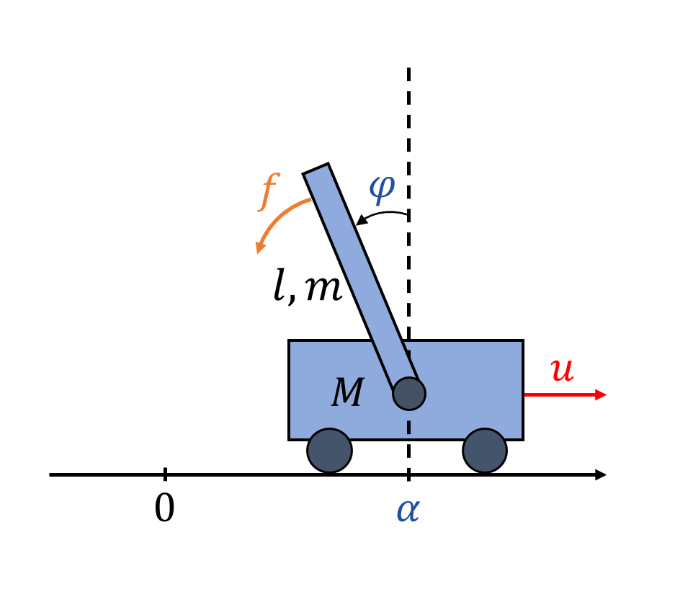
\includegraphics[width=0.5\linewidth]{figs/cart.png}
    \caption{Перевернутый маятник на тележке}
    \label{fig:cart}
\end{figure}

% \begin{tikzpicture}[line width=1pt]

% % Тележка
% \draw[fill=blue!20] (-2,0) rectangle (2,1); % Прямоугольник тележки
% \draw[thick] (-2,0) -- (2,0); % Основание тележки

% % Колёса
% \draw[fill=black] (-1.5,-0.5) circle (0.5); % Левое колесо
% \draw[fill=black] (1.5,-0.5) circle (0.5);  % Правое колесо

% % Маятник
% \draw[thick, red] (0,1) -- (-0.7,3); % Стержень маятника
% \draw[fill=red] (-0.7,3) circle (0.1); % Конец маятника

% % Угол
% \draw[thick, ->] (0.3,1.2) arc[start angle=20, end angle=115, radius=0.6];
% \node[right] at (0.6,1.6) {$\phi$};

% % Подписи
% \node[below] at (0,-0.2) {Тележка};
% \node[right] at (-0.7,3.2) {Маятник};

% % Координатная ось
% \draw[->] (0,0) -- (0,4) node[above] {$y$}; % Ось y
% \draw[->] (0,0) -- (3,0) node[right] {$x$}; % Ось x

% \end{tikzpicture}

Построим математическую модель перевернутого маятника на тележке, 
представленного на Рисунке~\ref{fig:cart}. В качестве переменных состояния выберем:
\begin{itemize}
    \item $x_1 = a$~--- линейная координата тележки,
    \item $x_2 = \dot{a}$~--- скорость тележки,
    \item $x_3 = \varphi$~--- угол отклонения маятника от вертикали,
    \item $x_4 = \dot{\varphi}$~--- угловая скорость маятника.
\end{itemize}

В качестве управляющей переменной примем $u$~--- горизонтальную силу,
 приложенную к тележке. Внешнее возмущение $f$ представлено вращающим 
 моментом, действующим на маятник. Выходные (измеряемые) переменные:
\begin{itemize}
    \item $y_1 = a$,\
    \item $y_2 = \varphi$.
\end{itemize}

При построении математической модели будем считать, что трение отсутствует, 
а масса маятника равномерно распределена вдоль стержня.
Я выведения модели воспользуемся ходом мысли из \cite{pendulum_cart}.
Введем пару обозначений:
\begin{itemize}
    \item $r = l/2$~--- расстояние от крепления маятника до его центра масс,
    \item $J_p = \frac{ml^2}{12}+mr^2$~--- момент инерции маятника из крепления маятника.
    \item $k=(M+m)J_p-(mr)^2$~--- коэффициент, который будет часто встречаться.
\end{itemize}
Координату по оси $X$ центра масс маятника $a_p$ можно выразить следующим образом:
\begin{equation*}
    a_p=a-r\sin\varphi,
\end{equation*}
возьмем вторую производную по времени:
\begin{equation}
    \label{eq:xp}
    \ddot a_p=\ddot a-r(\ddot\varphi\cos\varphi-\dot\varphi^2\sin\varphi).
\end{equation}
Воспользуется вторым законом Ньютона, расписав его как для тележки, так и для маятника:
\begin{equation}
    \label{eq:N}
    M\ddot a+m\ddot a_p=u.
\end{equation}
Подставим \eqref{eq:xp} в \eqref{eq:N}:
\begin{equation*}
    (M+m)\ddot a-mr(\ddot\varphi\cos\varphi-\dot\varphi^2\sin\varphi)=u,
\end{equation*}
откуда выразим ускорение тележки:
\begin{equation}
    \label{eq:x}
    \ddot a=\frac{1}{M+m}(u+mr(\ddot\varphi\cos\varphi-\dot\varphi^2\sin\varphi)).
\end{equation}
Рассмотрим баланс моментов из системы координат связанной с тележкой в центре крепления маятника:
\begin{equation*}
    J_p\ddot\varphi=mgr\sin\varphi+m\ddot ar\cos\varphi+f,
\end{equation*}
имеем моменты от силы притяжения Земли, от двигающейся системы координат и внешний момент.
Получим формулу для углового ускорения:
\begin{equation}
    \label{eq:phi}
    \ddot\varphi=\frac{1}{J_p}(f+mr(g\sin\varphi+\ddot a\cos\varphi)).
\end{equation}
Подставим \eqref{eq:phi} в \eqref{eq:x} и получим:
\begin{equation*}
    \ddot a=\frac{1}{M+m}\left(u+mr\left(\frac{\cos\varphi}{J_p}(f+mr(g\sin\varphi+\ddot a\cos\varphi))-\dot\varphi^2\sin\varphi\right)\right),
\end{equation*}
\begin{equation*}
    (M+m)J_p\ddot a=J_pu+mrf\cos\varphi+(mr)^2g\cos\varphi\sin\varphi
    +(mr)^2\ddot a\cos^2\varphi-mrJ_p\dot\varphi^2\sin\varphi,
\end{equation*}
\begin{equation}
    \label{eq:xx}
    \ddot a=\frac{1}{(M+m)J_p-(mr\cos\varphi)^2}\cdot\Big[J_p(u-mr\dot\varphi^2\sin\varphi)+(f+mrg\sin\varphi)(mr)\cos\varphi\Big],
\end{equation}
и, подставив \eqref{eq:xx} обратно в \eqref{eq:phi}, получим
\begin{multline}
    \label{eq:phiphi}
    \ddot\varphi=\frac{1}{J_p}\Bigg(f+mrg\sin\varphi+\frac{mr\cos\varphi}{(M+m)J_p-(mr\cos\varphi)^2}\cdot\\ 
    \Big[J_p(u-mr\dot\varphi^2\sin\varphi)+(f+mrg\sin\varphi)mr\cos\varphi\Big] \Bigg).
\end{multline}
Таким образом имеем следующую систему
\begin{equation}
    \label{eq:origsys}
    \begin{cases}
        \dot x_1 = \dot a,\\
        \dot x_2 = F_2(x_3, x_4, f, u)\text{ ~-- \eqref{eq:xx}},\\
        \dot x_3 = \dot\varphi,\\
        \dot x_4 = F_4(x_3, x_4, f, u)\text{ ~-- \eqref{eq:phiphi}}.
    \end{cases}
\end{equation}


\section{Точки равновесия}

Найдем все точки равновесия объекта при $u,\ f\equiv0$. В точках равновесия производная состояния
равна нулю:
\begin{equation*}
    \begin{cases}
        \dot x_1 = \dot a = 0,\\
        \dot x_2 = F_2(x_3, x_4, 0, 0)= 0,\\
        \dot x_3 = \dot\varphi=0,\\
        \dot x_4 = F_4(x_3, x_4, 0, 0)=0.
    \end{cases}
\end{equation*}
Рассмотрим \eqref{eq:xx}:
\begin{equation*}
    0=\frac{1}{(M+m)J_p-(mr\cos\varphi)^2}\cdot
    \Big[J_p(0-mr0\sin\varphi)+(0+mrg\sin\varphi)mr\cos\varphi\Big],
\end{equation*}
так знаменатель строго положителен, спокойно приравниваем числитель к нулю:
\begin{equation*}
    \cos\varphi\sin\varphi=0,
\end{equation*}
решением этого уравнения является $\varphi=\pi n/2,\ n\in\mathbb{Z}$.
Вместо \eqref{eq:phiphi} рассмотрим \eqref{eq:phi}, так как $\ddot a=0$:
\begin{equation*}
    0=\frac{1}{J_p}(0+mrg\sin\varphi+mr0\cos\varphi),
\end{equation*}
\begin{equation*}
    sin\varphi=0\quad\Rightarrow\quad\varphi=\pi n,\ n\in\mathbb{Z}.
\end{equation*}
Значит итоговое решение для точек равновесия будет любая координата $a$ и угол маятника $\varphi$
равный $0^\circ $ или $180^\circ $ при $\varphi\in[0^\circ;360^\circ)$, что логично, если представлять
маятник в голове, отсюда же очивидно, что при $\varphi=0$ точка равновесия неустойчивая, а при 
$\varphi=180^\circ$ устойчивая.


\section{Линеаризация}

Линеаризируем уравнения объекта, около неустойчивой точки равновесия $\varphi=0$, взяв 
$\cos\varphi\approx1,\ \sin\varphi\approx\varphi,\ \dot\varphi^2\approx0$.
Тогда \eqref{eq:xx} преобразуется в
\begin{equation}
    \label{lx}
    \ddot a=\frac{1}{k}
    \Big[J_pu+(f+mrg\varphi)mr\Big],
\end{equation}
а уравнение \eqref{eq:phiphi} в 
\begin{equation*}
    \ddot\varphi=\frac{1}{J_p}\Bigg(f+mrg\varphi+\frac{mr}{k}
    \Big[J_pu+(f+mrg\varphi)mr\Big] \Bigg),
\end{equation*}
\begin{equation*}
    \ddot\varphi=\frac{mr}{kJ_p}\Big(\frac{k}{mr}f+kg\varphi+
    J_pu+mrf+(mr)^2g\varphi\Big),
\end{equation*}
\begin{equation*}
    \ddot\varphi=\frac{mr}{kJ_p}\Big(
        ((mr)^2+k)g\varphi+J_pu+(mr+\frac{k}{mr})f
    \Big),
\end{equation*}
\begin{equation}
    \label{eq:lphi}
    \ddot\varphi=\frac{mr}{k}\Big(
        (M+m)g\varphi+u\Big)+\frac{M+m}{k}f
    .
\end{equation}
Таким образом, можем получить систему ВСВ:
\begin{equation}
    \label{eq:sys}
    \begin{cases}
        \dot x=Ax+Bu+Df,\\
        y=Cx,
    \end{cases}
\end{equation}
где
\begin{equation*}
    A=\begin{bmatrix}
        0&1&0&0\\
        0&0&\dfrac{g}{k}(mr)^2&0\\
        0&0&0&1\\
        0&0&\dfrac{M+m}{k}mrg&0
    \end{bmatrix},\quad
    B=\begin{bmatrix}
        0\\\dfrac{J_p}{k}\\0\\\dfrac{mr}{k}
    \end{bmatrix},\quad
    D=\begin{bmatrix}
        0\\\dfrac{mr}{k}\\0\\\dfrac{M+m}{k}
    \end{bmatrix},\quad
    C=\begin{bmatrix}
        1&0&0&0\\
        0&0&1&0
    \end{bmatrix}.
\end{equation*}


\section{Выбор исходных данных}

Согласно варианту пусть
\begin{itemize}
    \item ускорение свободного падения $g=9.81$~м/с$^2$,
    \item масса тележки $M=487.29$~кг,
    \item масса маятника $m=8.12$~кг,
    \item длина маятника $l=3.50$~м,
    \item расстояние от крепления до центра масс $r=l/2=1.75$~м,
    \item момент инерции маятника относительно оси крепления $J_p=\frac{ml^2}{12}+mr^2=33.16$~кг$\cdot$м$^2$.
    \item коэффициент $k=(M+m)J_p-(mr)^2=16224.22$~кг$^2\cdot$м$^2$.
\end{itemize}

\chapter{Анализ математической модели}

\section{Анализ матриц}

Cобственные числа матрицы А:
\begin{equation*}
\left\{\begin{array}{cccc}
0&
0&
2.063&
-2.063
\end{array}\right\}
\end{equation*}
и матрица из собственных векторов матрицы А:
\begin{equation*}
    \begin{bmatrix}
1.0 & -1.0 & 0.01251 & -0.01251\\
0 & \text{4.008e-292} & 0.0258 & 0.0258\\
0 & 0 & 0.436 & -0.436\\
0 & 0 & 0.8995 & 0.8995
\end{bmatrix}.
\end{equation*}
Как видно из собственных чисел, система неустойчива.
Матрица наблюдаемости пары $(C,\ A)$
\begin{equation*}
    V=\begin{bmatrix}
1.0 & 0 & 0 & 0\\
0 & 0 & 1.0 & 0\\
0 & 1.0 & 0 & 0\\
0 & 0 & 0 & 1.0\\
0 & 0 & 0.1221 & 0\\
0 & 0 & 4.257 & 0\\
0 & 0 & 0 & 0.1221\\
0 & 0 & 0 & 4.257
    \end{bmatrix}
\end{equation*}
имеет ранг 4, значит система \eqref{eq:sys} полностью наблюдаема и, как следствие, обнаруживаема.
Матрица управляемости пары $(A,\ B)$
\begin{equation*}
    U=\begin{bmatrix}
0 & 0.002044 & 0 & 0.0001069\\
0.002044 & 0 & 0.0001069 & 0\\
0 & 0.0008759 & 0 & 0.003728\\
0.0008759 & 0 & 0.003728 & 0
    \end{bmatrix}
\end{equation*}
тоже имеет ранг 4, значит система \eqref{eq:sys} полностью управляема и, как следствие, стабилизируема.

\section{Передаточные функции}

Найдем передаточную матрицу (ПМ) от $u$ к $y$, для этого можем опустить $f$, так как система линейная,
и рассмотрим систему \eqref{eq:sys} в виде:
\begin{equation*}
    \begin{cases}
        \dot x=Ax+Bu,\\
        y=Cx,
    \end{cases}
\end{equation*}
после чего воспользуемся формулой:
\begin{equation*}
    \underset{u\rightarrow y}{W}(s)=C(sI-A)^{-1}B=
    \begin{bmatrix}
        \dfrac{\text{9.123e-6}\,{\left(\text{2.522e+17}\,s^2 -\text{1.06e+18}\right)}}{s^2 \,{\left(\text{1.126e+15}\,s^2 -\text{4.793e+15}\right)}}\\[2ex]
        \dfrac{\text{9.861e+11}}{\text{1.126e+15}\,s^2 -\text{4.793e+15}}
    \end{bmatrix}=
    \begin{bmatrix}
        W_{u_1}(s)\\W_{u_2}(s)
    \end{bmatrix}.
\end{equation*}
Рассмотрим $W_{u_1}(s)$, она имеет АДП (абсолютный динамический порядок) 4 и ОДП (относительный динамический порядок) 2;
нули $\left\{\begin{array}{cc}
-2.05&
2.05
\end{array}\right\}$ и полюса $\left\{\begin{array}{cccc}
0&
0&
-2.063&
2.063
\end{array}\right\}.$
Рассмотрим $W_{u_2}(s)$, она имеет АДП 2 и ОДП 2;
нулей нет, а полюса $\left\{\begin{array}{cc}
-2.063&
2.063
\end{array}\right\}.$

Найдем ПМ от $f$ к $y$, опустим $u$ и рассмотрим систему \eqref{eq:sys} в виде:
\begin{equation*}
    \begin{cases}
        \dot x=Ax+Df,\\
        y=Cx,
    \end{cases}
\end{equation*}
после чего воспользуемся формулой:
\begin{equation*}
    \underset{f\rightarrow y}{W}(s)=C(sI-A)^{-1}D=
    \begin{bmatrix}
\dfrac{\text{1.906e-19}\,{\left(\text{7.352e+31}\,s^2 -\text{3.825e+15}\right)}}{s^2 \,{\left(\text{1.126e+15}\,s^2 -\text{4.793e+15}\right)}}\\[2ex]
\dfrac{\text{4.885e+14}}{\text{1.126e+15}\,s^2 -\text{4.793e+15}}
    \end{bmatrix}=
    \begin{bmatrix}
        W_{f_1}(s)\\W_{f_2}(s)
    \end{bmatrix}.
\end{equation*}
Рассмотрим $W_{f_1}(s)$, она имеет АДП 4 и ОДП 2;
нули $\left\{\begin{array}{cc}
-\text{7.212e-9}&
\text{7.212e-9}
\end{array}\right\}$ и полюса $\left\{\begin{array}{cccc}
0&
0&
-2.063&
2.063
\end{array}\right\}.$
Рассмотрим $W_{f_2}(s)$, она имеет АДП 2 и ОДП 2;
нулей нет, а полюса $\left\{\begin{array}{cc}
-2.063&
2.063
\end{array}\right\}.$

Подытожим:
\begin{enumerate}
    \item Абсолютный динамический порядок (АДП):
        \begin{itemize}
            \item Для $W_{u_1}(s)$ - ПФ от управления к координате тележки: АДП равен 4, 
            что означает, что система имеет сложную динамику с четырьмя интеграторами.
            \item Для $W_{u_2}(s)$ - ПФ от управления к углу отклонения маятника: АДП равен 2, 
            что указывает на более простую динамику с двумя интеграторами.
            \item Для $W_{f_1}(s)$ - ПФ от возмущения к координате тележки: АДП равен 4.
            \item Для $W_{f_2}(s)$ - ПФ от возмущения к углу отклонения маятника: АДП равен 2.
        \end{itemize}
    \item Относительный динамический порядок (ОДП):
        \begin{itemize}
            \item Для $W_{u_1}(s)$ и $W_{u_2}(s)$: ОДП равен 2.
            \item Для $W_{f_1}(s)$ и $W_{f_2}(s)$: ОДП также равен 2.
        \end{itemize}
    \item Нули:
        \begin{itemize}
            \item Для $W_{u_1}(s)$: Нули $\{-2.05, 2.05\}$.
            \item Для $W_{u_2}(s)$: Нулей нет.
            \item Для $W_{f_1}(s)$: Нули $\{-\text{7.212e-9}, \text{7.212e-9}\}$.
            \item Для $W_{f_2}(s)$: Нулей нет.
        \end{itemize}
    \item Полюса:
        \begin{itemize}
            \item Для $W_{u_1}(s)$, $W_{f_1}(s)$: Полюса исходят из матрицы системы $A$ и расположены в $\{0, 0, -2.063, 2.063\}$, 
            есть нейсточивый полюс $2.063$, ПФ будут расходиться.
            \item Для  $W_{u_2}(s)$,  $W_{f_2}(s)$: Полюса исходят из матрицы системы $A$ и расположены в $\{-2.063, 2.063\}$, 
            есть нейсточивый полюс $2.063$, ПФ будут расходиться.
        \end{itemize}
\end{enumerate}

\section{Моделирование}

Выполним компьютерное моделирование свободного движения линеаризованного
объекта согласно уравнениям \eqref{eq:sys} при различных начальных условиях:
\begin{equation*}
    x_{01}=\begin{bmatrix}
        0.1\\
        -0.05\\
        0.02\\
        0.001
    \end{bmatrix},\quad
    x_{02}=\begin{bmatrix}
        0.05\\
         0.1\\
         -0.03\\
         0.001
    \end{bmatrix},\quad
    x_{03}=\begin{bmatrix}
        -0.02\\
        0.01\\
         0.1\\
         -0.001
    \end{bmatrix},
\end{equation*}
несильно отличающихся от нуля. При малом времени
моделирования результат можно увидеть на \autoref{fig:2.3.lin_free_t_low} 
и большом времени моделирования - на \autoref{fig:2.3.lin_free_t_high}.

\begin{figure}[H]
    \centering
    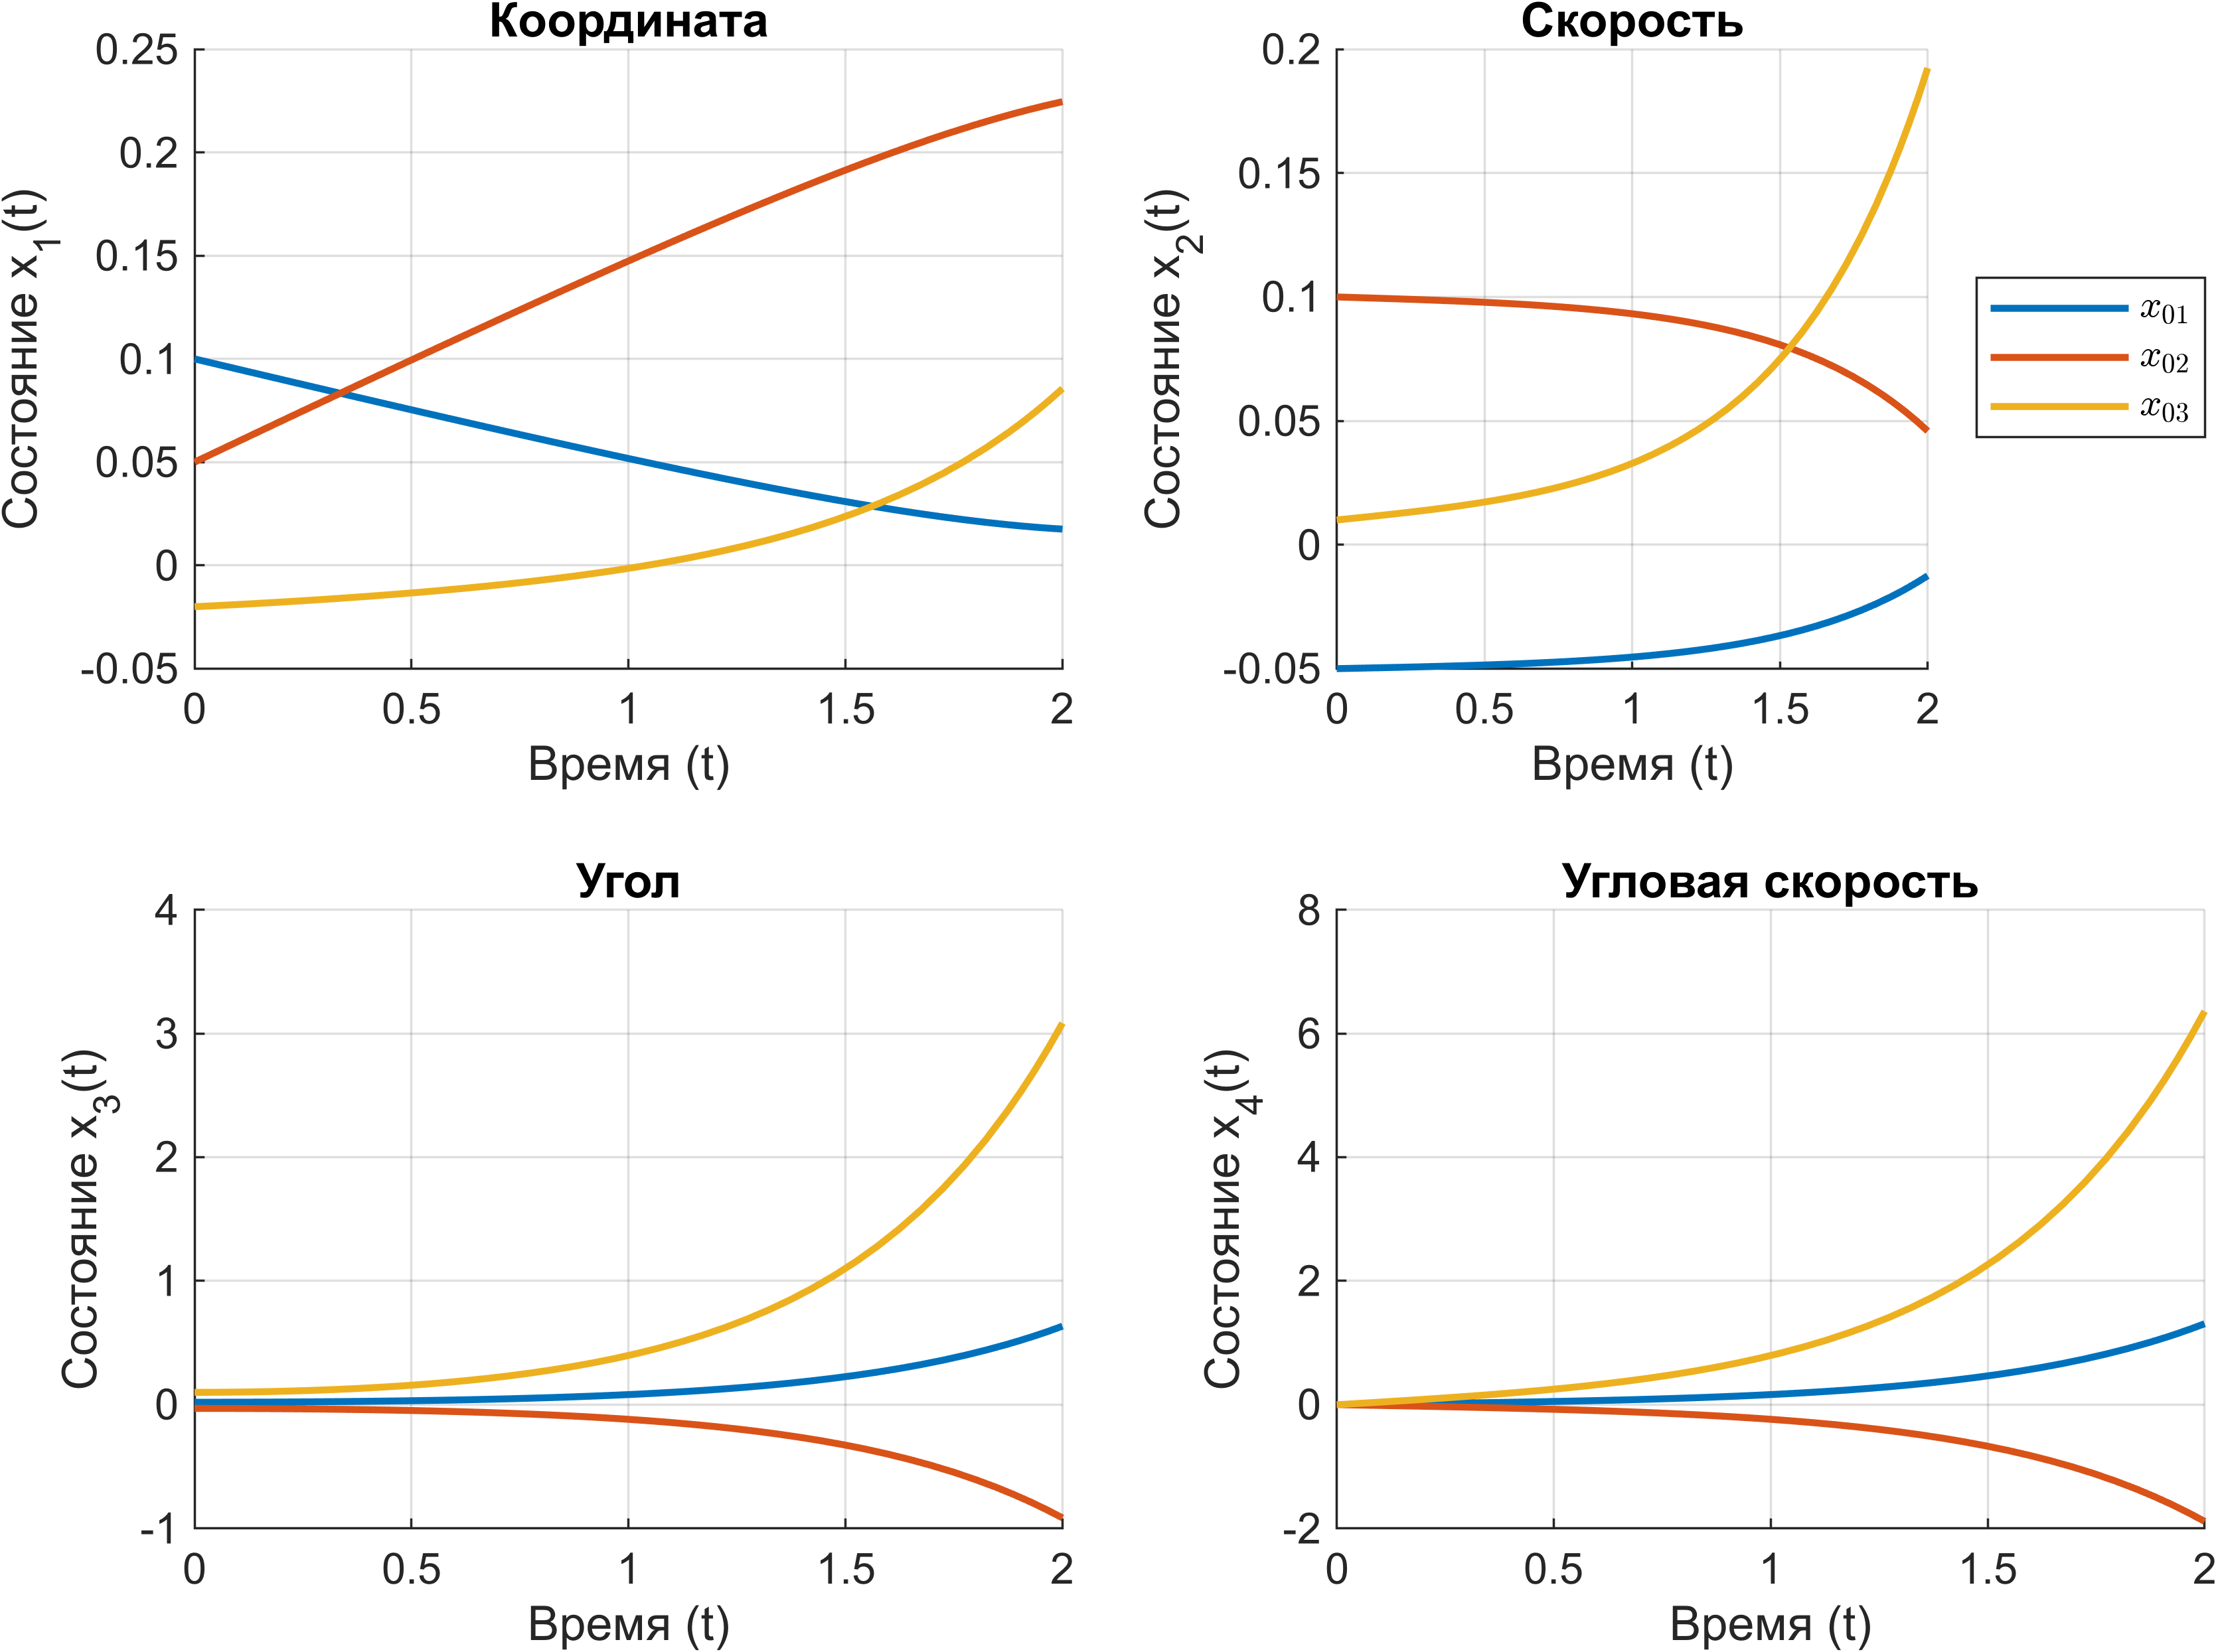
\includegraphics[width=\linewidth]{figs/2.3.lin_free_t_low.png}
    \caption{Моделирование свободного движения линеаризованного объекта
    при малом времени моделирования}
    \label{fig:2.3.lin_free_t_low}
\end{figure}
\begin{figure}[H]
    \centering
    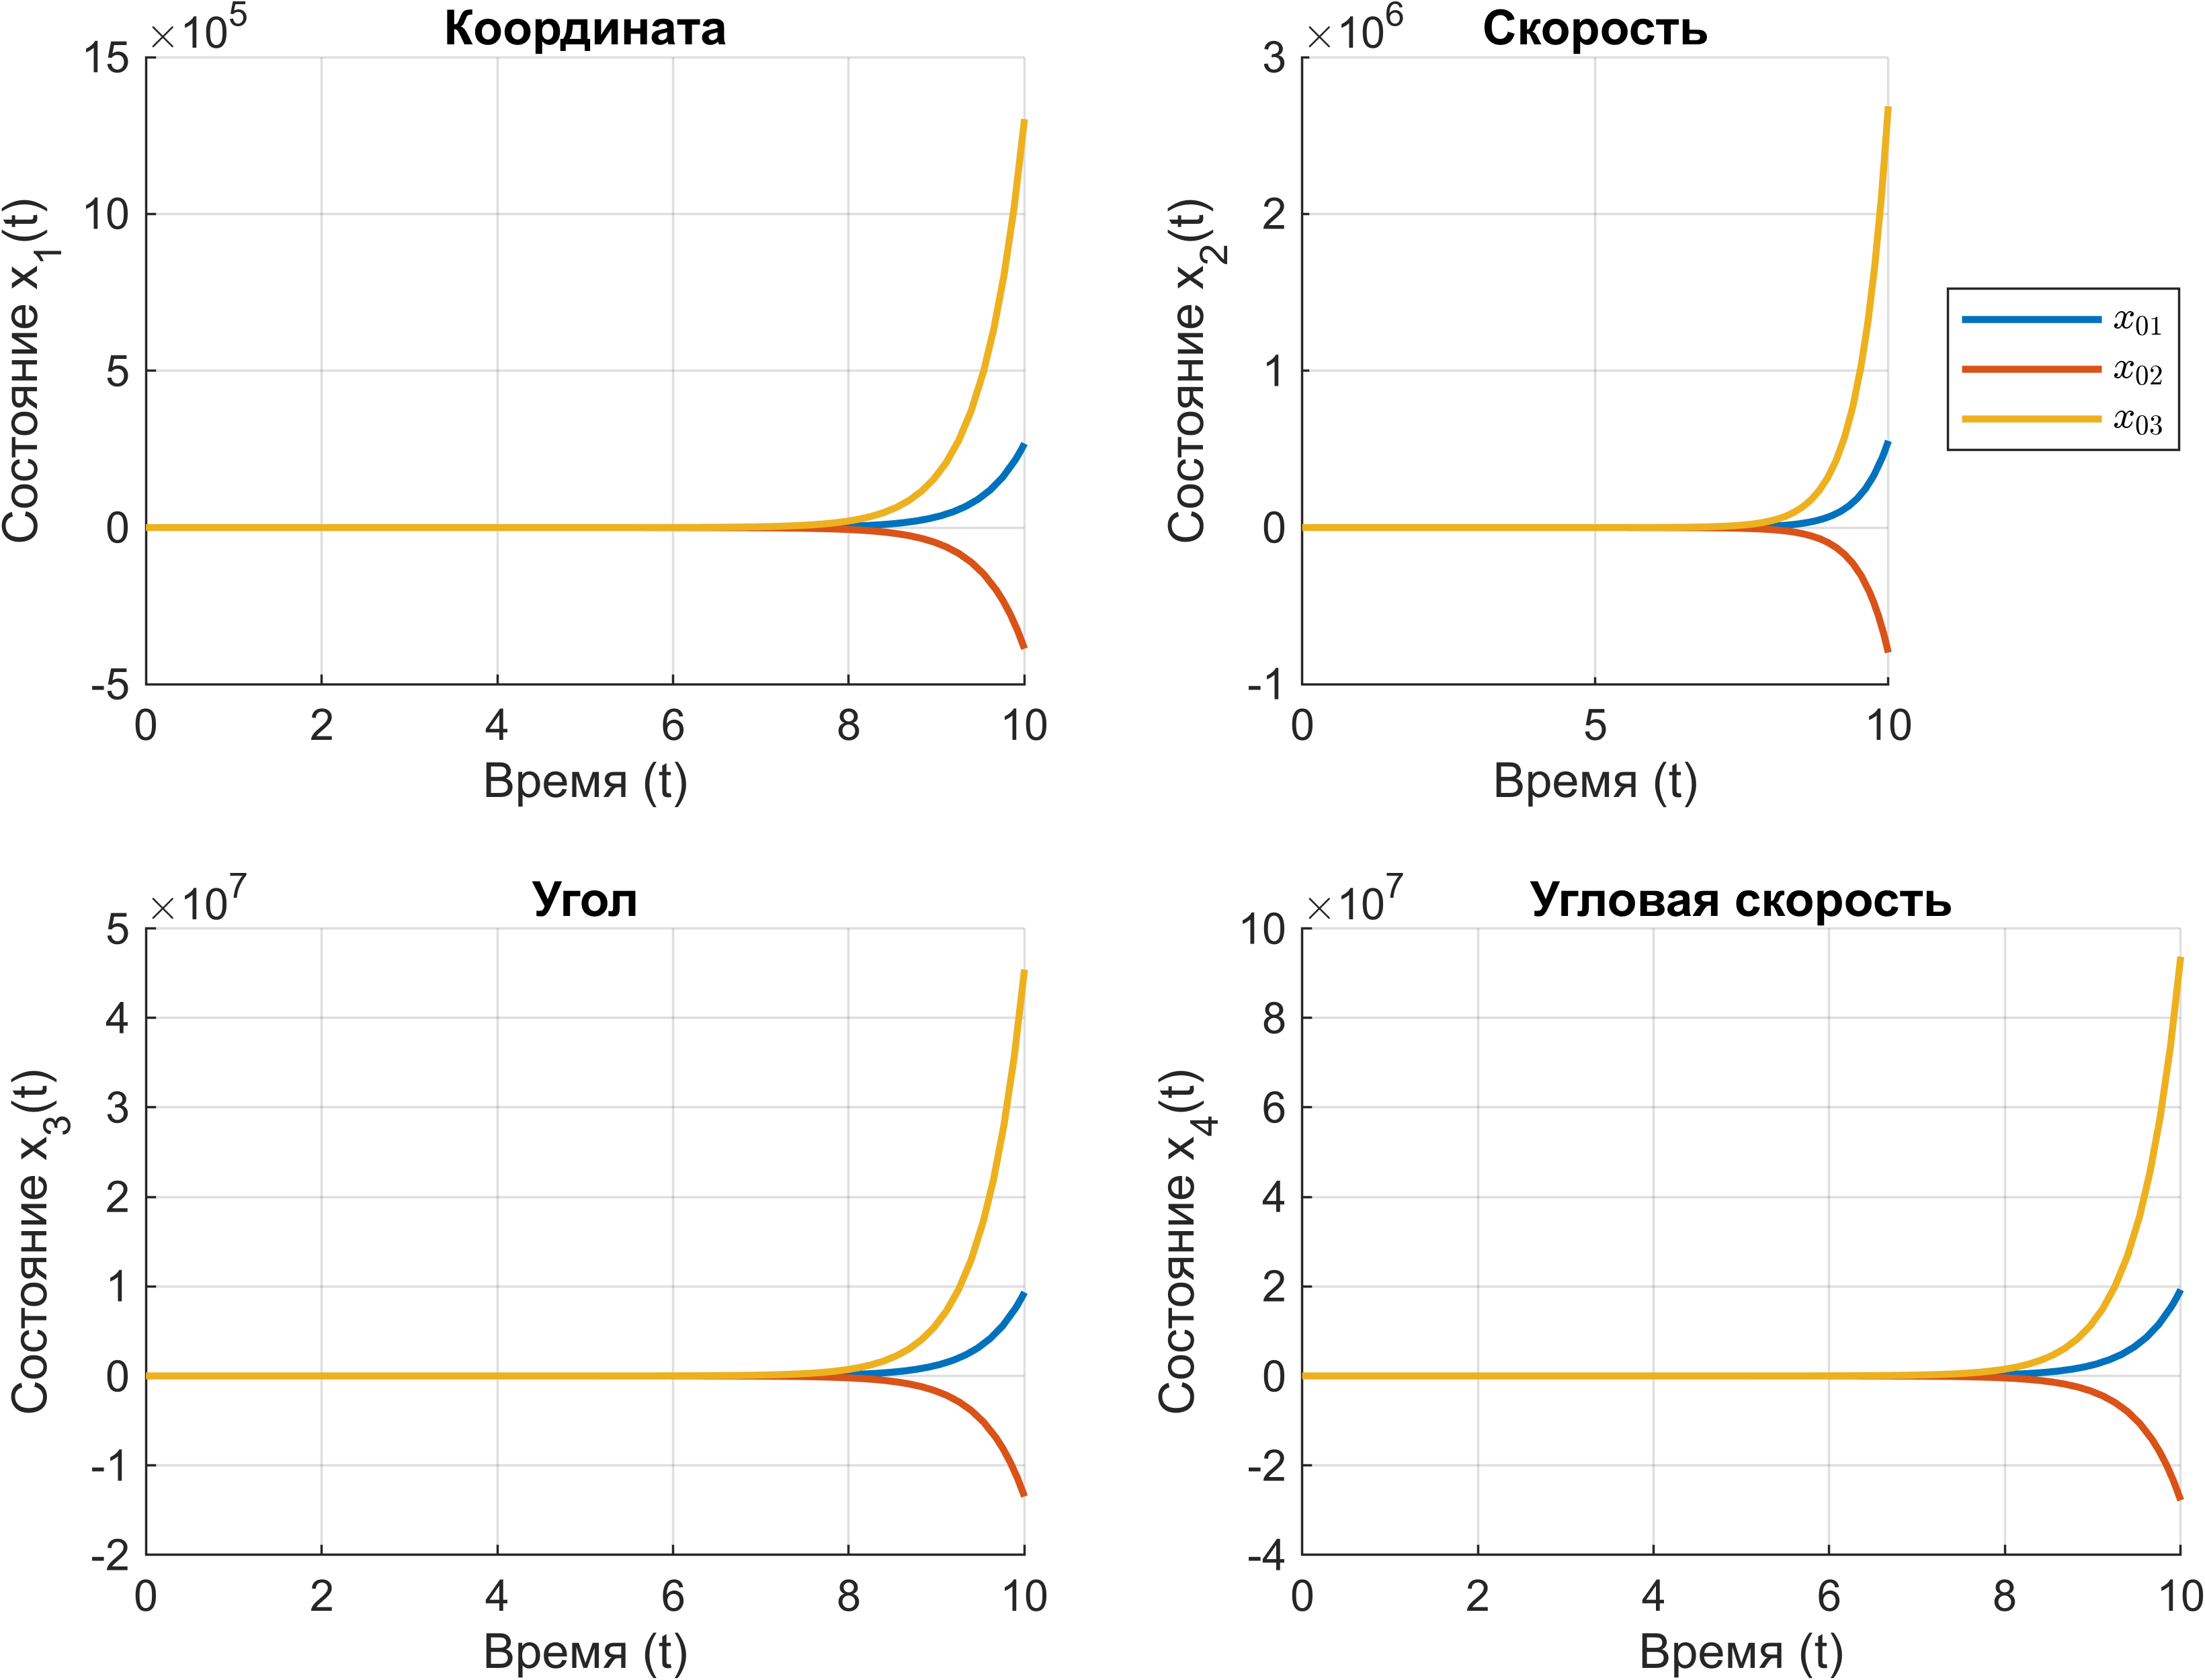
\includegraphics[width=\linewidth]{figs/2.3.lin_free_t_high.png}
    \caption{Моделирование свободного движения линеаризованного объекта
    при большом времени моделирования}
    \label{fig:2.3.lin_free_t_high}
\end{figure}

\noindent Выполним моделирование свободного движения объекта согласно уравнениям \eqref{eq:origsys}
при ранее выбранных начальных условиях. При малом времени
моделирования результат можно увидеть на \autoref{fig:2.3.nonlin_free_t_low} 
и большом времени моделирования - на \autoref{fig:2.3.nonlin_free_t_high}.
\noindent Как видно из графиков, при малом времени моделирования системы ведут себя очень похоже,
при большом времени моделирования система, описанная линеаризованной моделью, расходится по всем состояниям,
а система, описанная не линеаризованной моделью, имеет колеблюшиеся скорости, что ожидаемо, так как
никаких сил сопротивления нет, и постепенно расходящиеся
координату и угол с видными колебаниями, и, в зависимости от начальных условий, координата тележки уходит
в право или влево.

\begin{figure}[H]
    \centering
    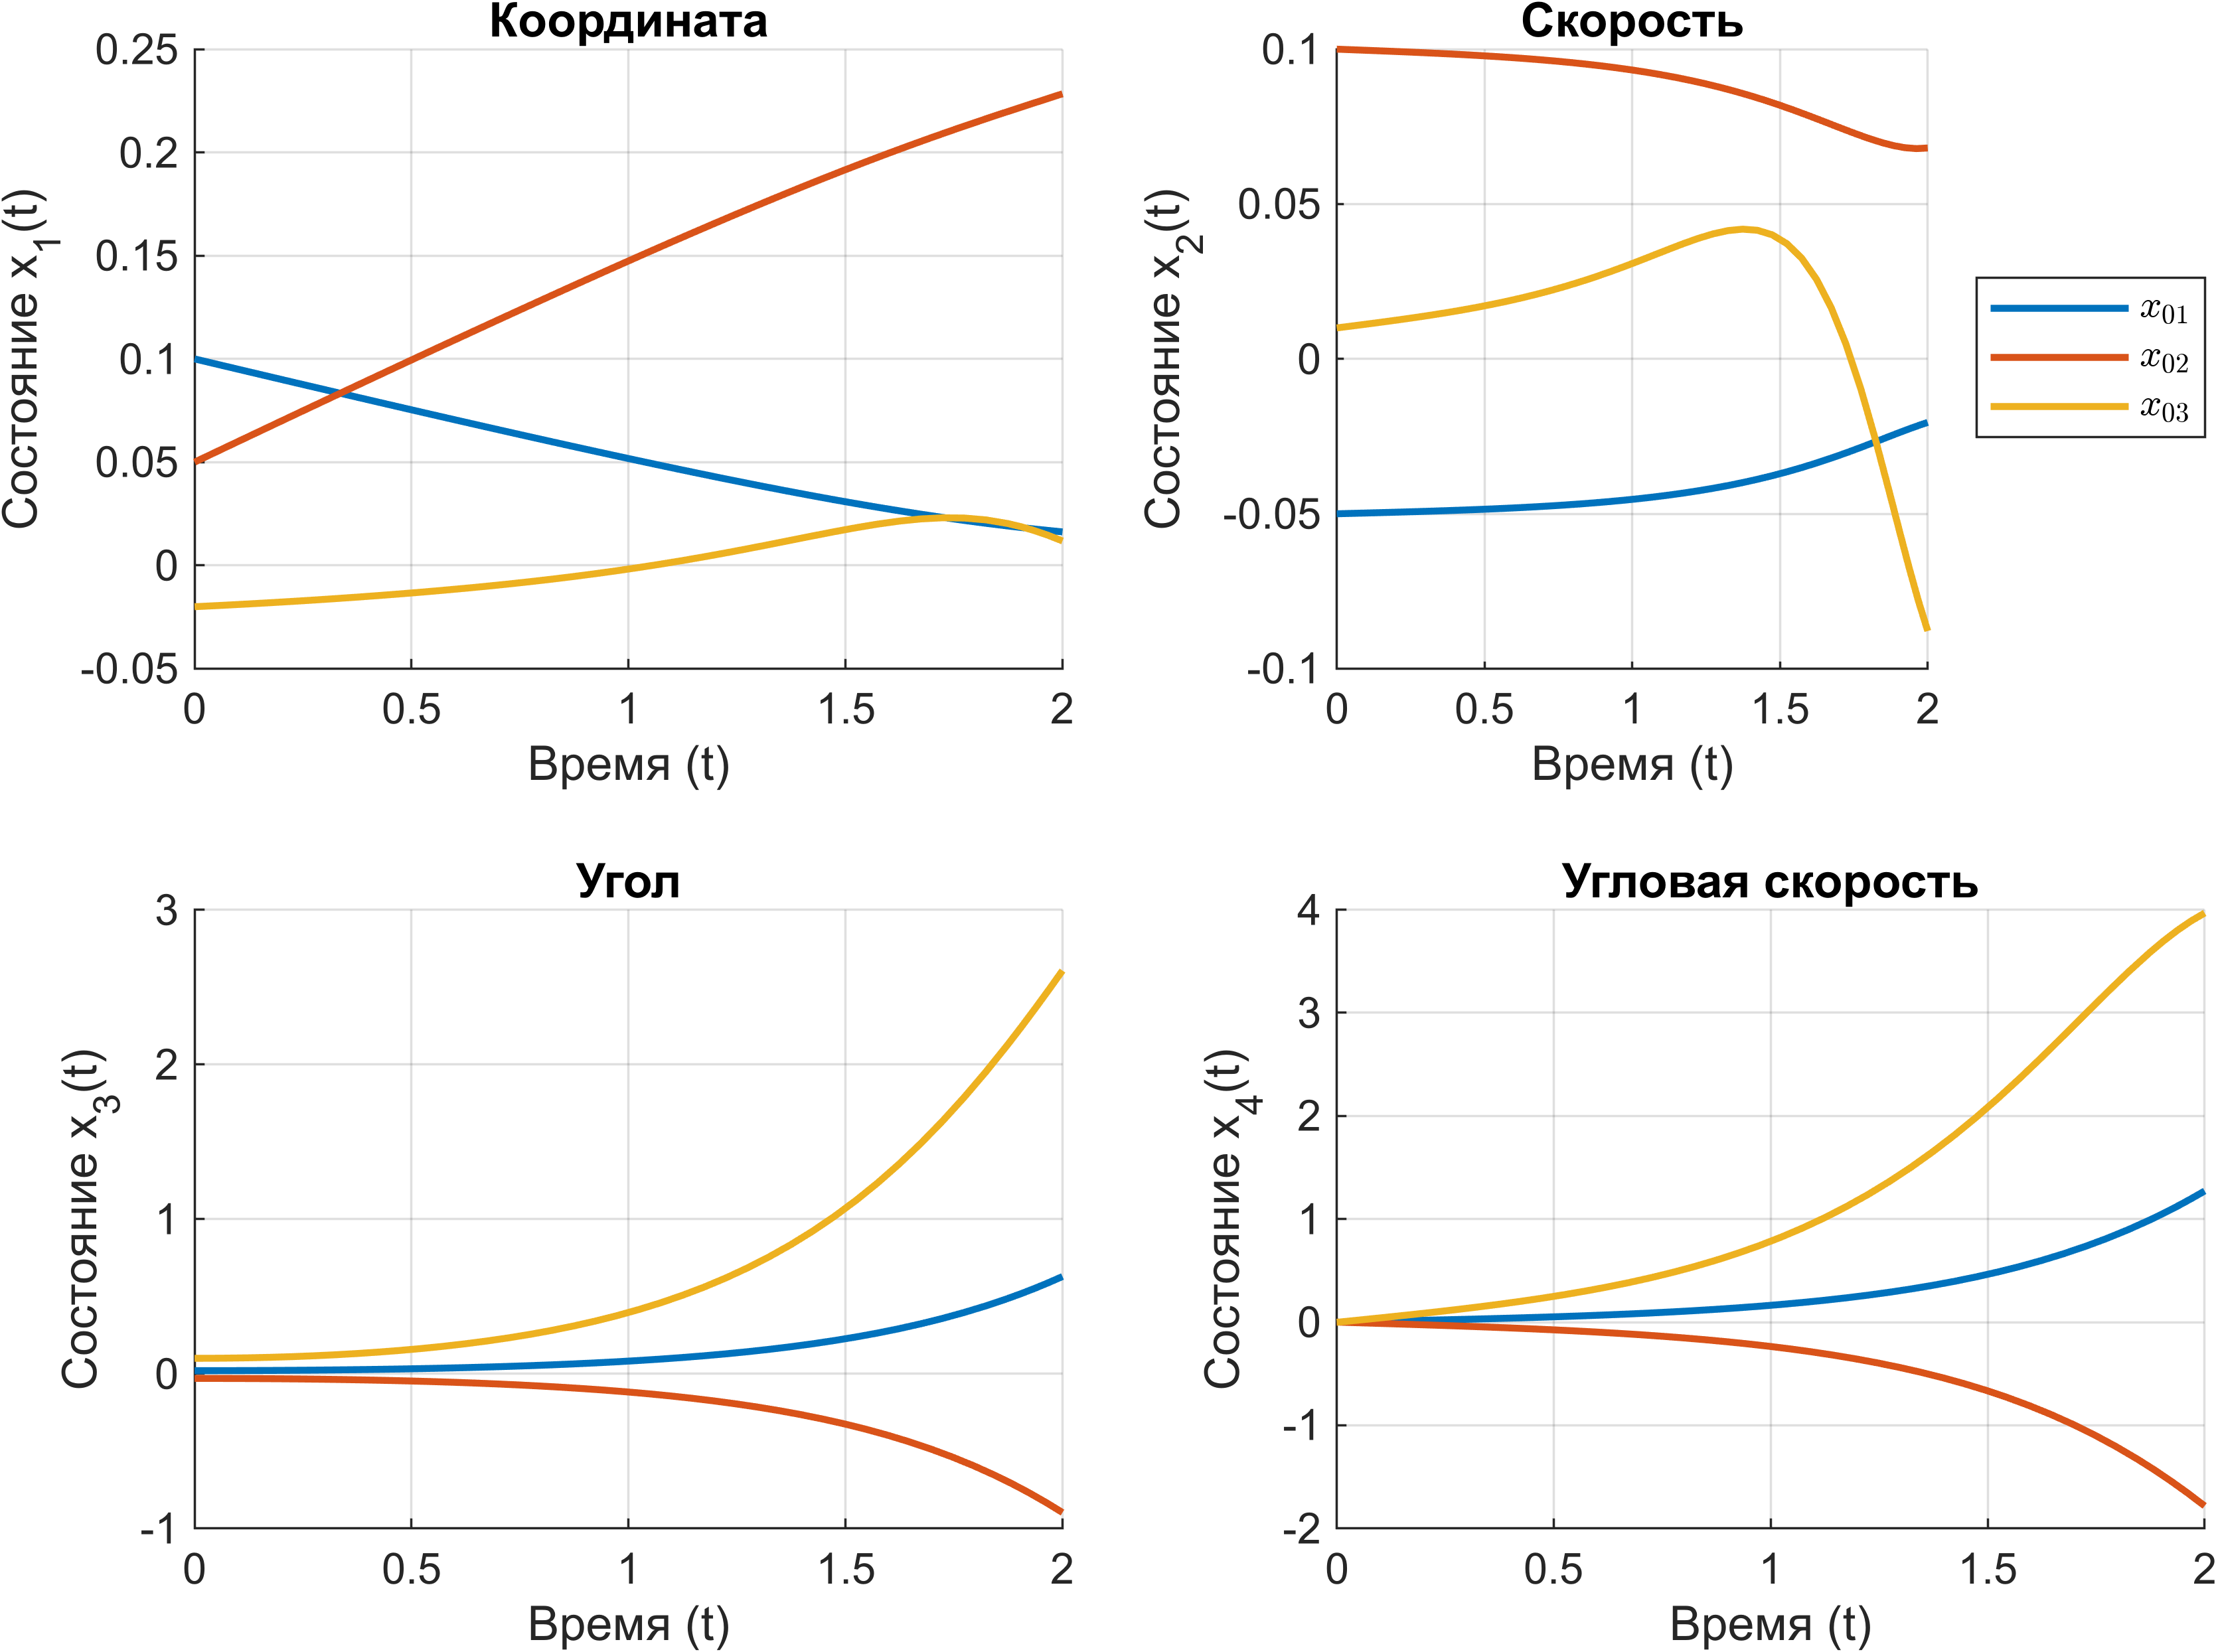
\includegraphics[width=0.8\linewidth]{figs/2.3.nonlin_free_t_low.png}
    \caption{Моделирование свободного движения не линеаризованного объекта
    при малом времени моделирования}
    \label{fig:2.3.nonlin_free_t_low}
\end{figure}
\begin{figure}[H]
    \centering
    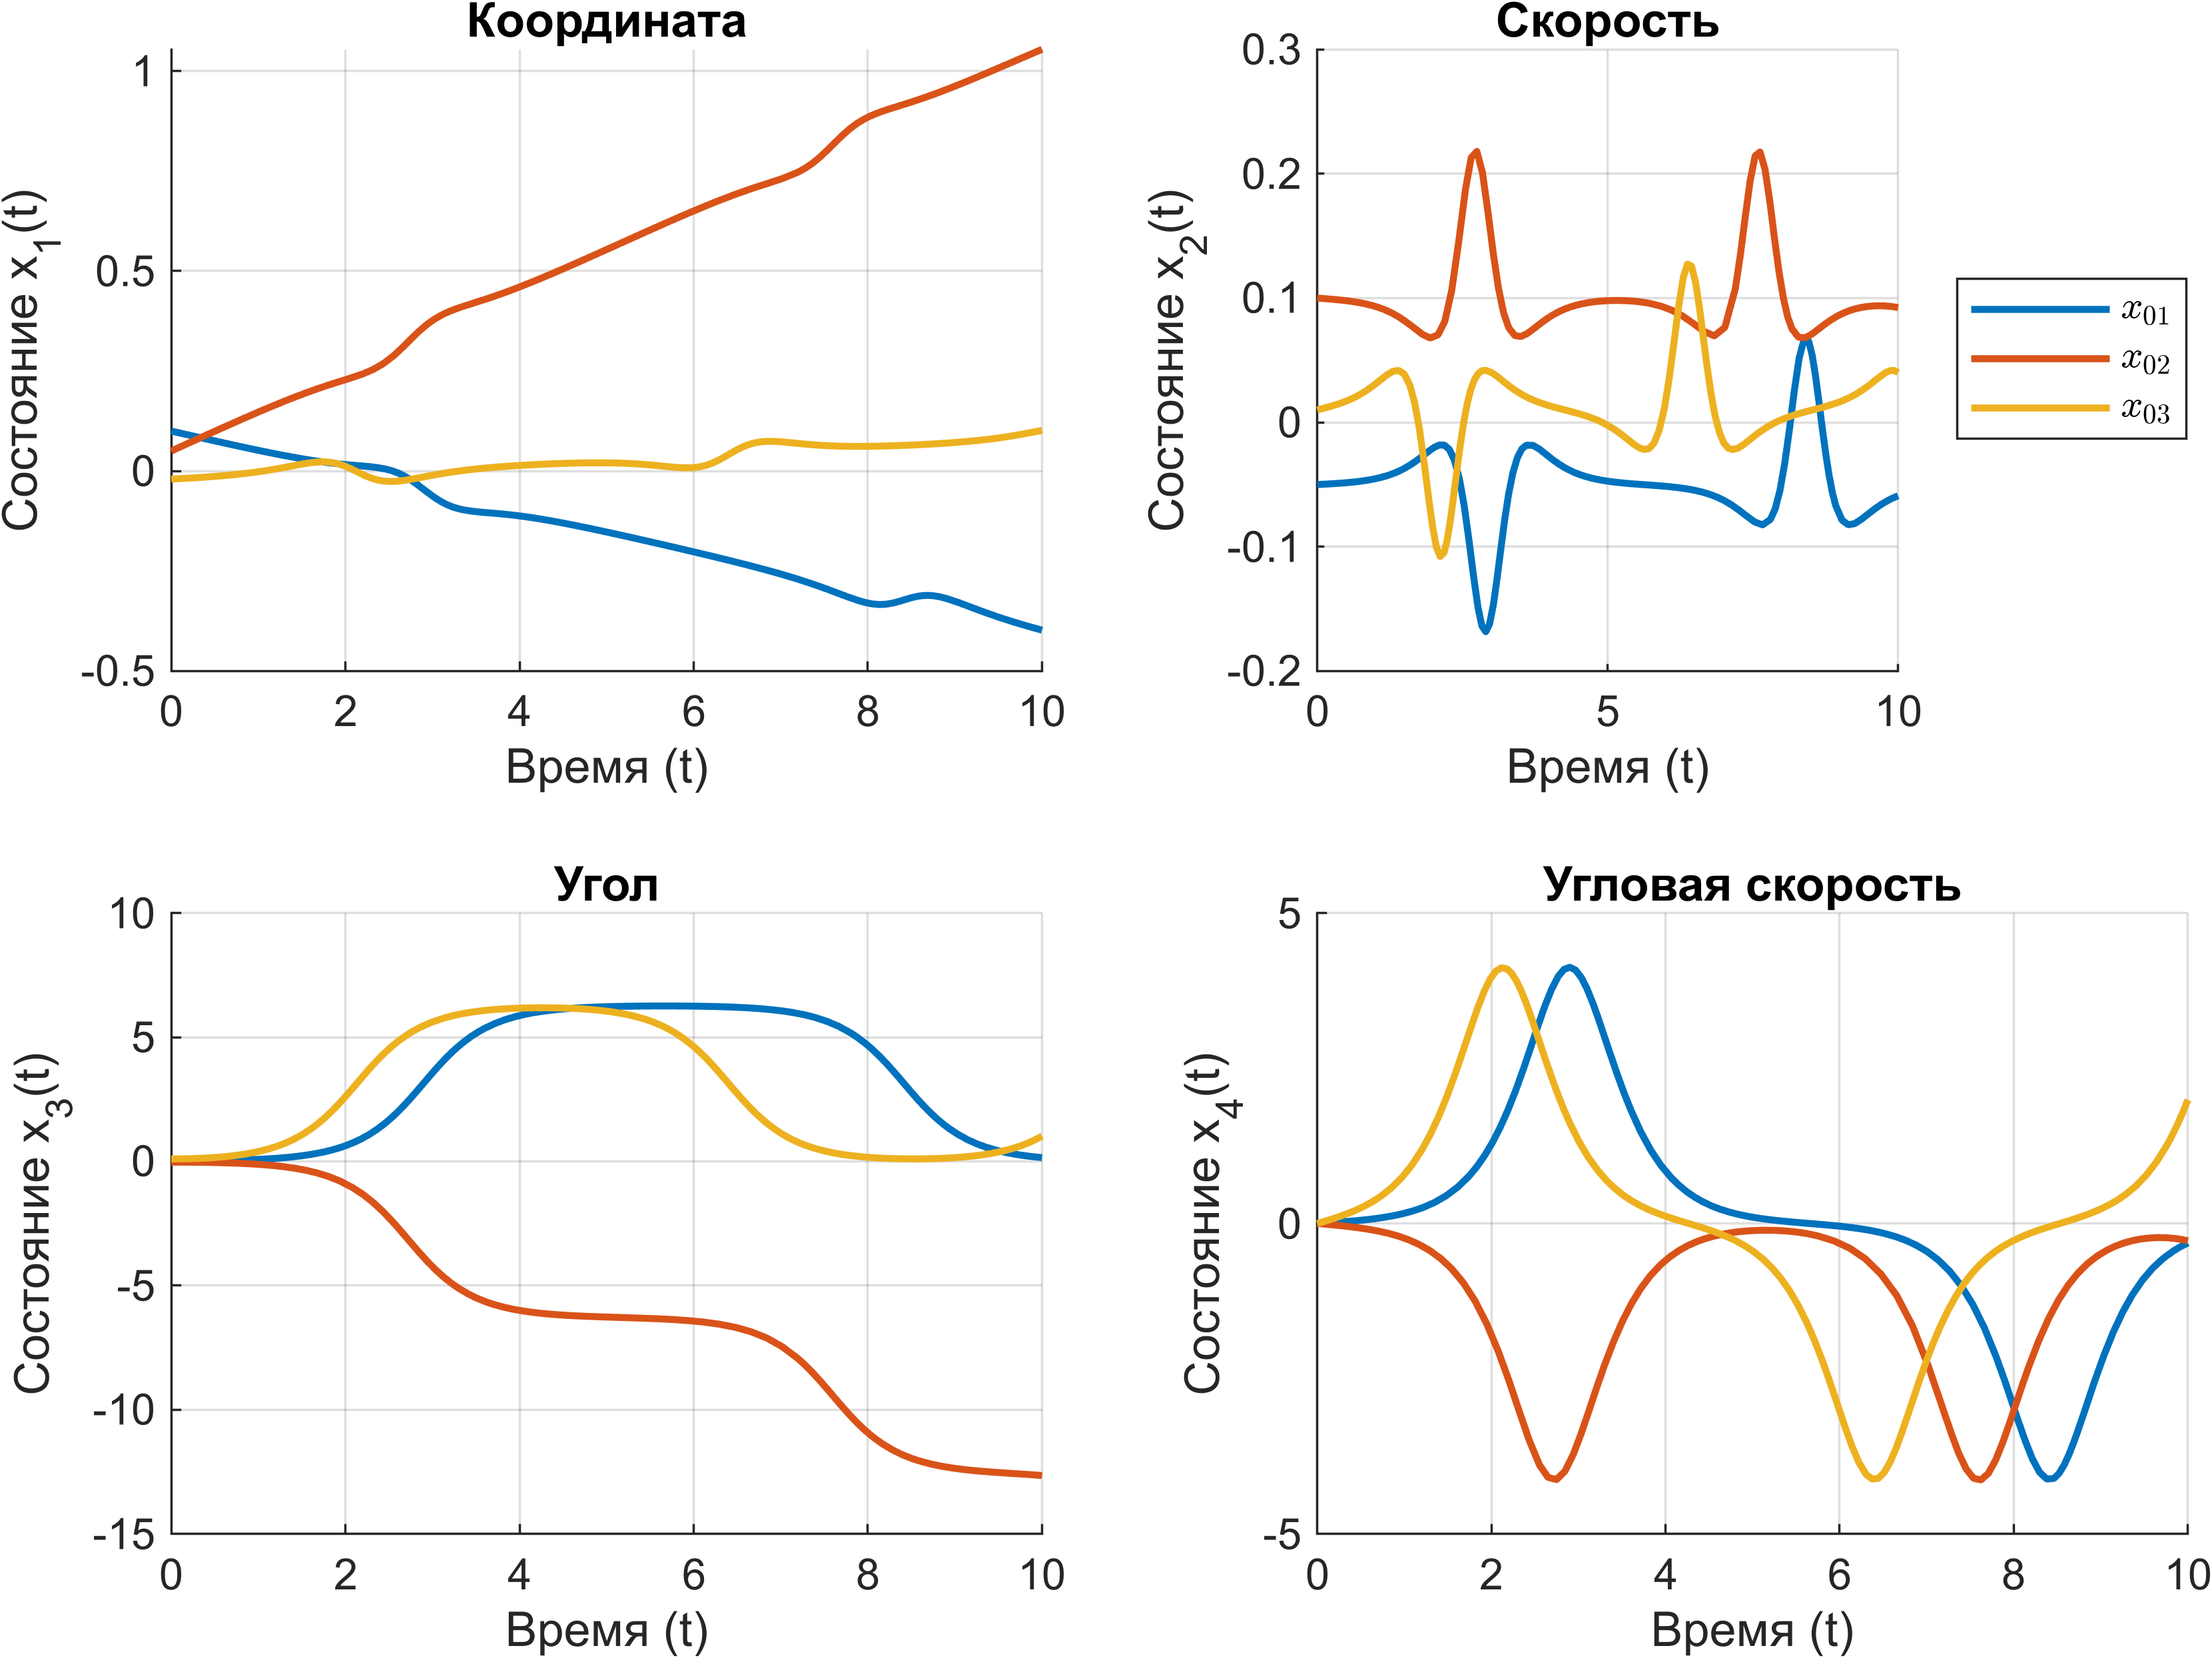
\includegraphics[width=0.8\linewidth]{figs/2.3.nonlin_free_t_high.png}
    \caption{Моделирование свободного движения не линеаризованного объекта
    при большом времени моделирования}
    \label{fig:2.3.nonlin_free_t_high}
\end{figure}

\chapter{Стабилизация маятника: модальное управление}

\section{Синтез регулятора по состоянию}

С помощью решения уравнения Сильвестра
\begin{equation}
    \label{eq:3.1.synv}
    AP-P\Gamma=BY
\end{equation}
произведем расчет регулятора
\begin{equation}
    \label{eq:3.1.reg}
    u=Kx.
\end{equation}
Выберем матрицу $\Gamma$, что бы ее спектр не пересекался со спектром матрицы $A$,
и матрицу $Y$ так, что бы пара $(Y,\ \Gamma)$ была наблюдаемой:
\begin{equation*}
    \Gamma=\begin{bmatrix}
        -1 & 0 & 0 & 0\\
        0 & -2 & 0 & 0\\
        0 & 0 & -3 & 0\\
        0 & 0 & 0 & -4
    \end{bmatrix},\quad
    Y=\begin{bmatrix}
        1&1&1&1
    \end{bmatrix}.
\end{equation*}
Используя CVX, получаем:
\begin{equation*}
    K=-YP^{-1}=\begin{bmatrix}
        2793.0 & 5819.0 & -51340.0 & -25000.0
    \end{bmatrix}
\end{equation*}
Спектр замкнутой системы $\sigma(A+BK)=\left\{\begin{array}{cccc}
-4.0 & -3.0 & -2.0 & -1.0
\end{array}\right\},$ регулятор синтезирован успешно.
Исследуем работоспособность синтезированного регулятора
при управлении нелинейной системой \eqref{eq:origsys}
в отсутствии внешних возмущений $f$. 
Рассмотрим 4 начальных условия:
\begin{equation*}
    x_{01}(0)=\begin{bmatrix}
        17\\
        0.1\\
        0.1\\
        0.1
    \end{bmatrix},\quad
    x_{02}(0)=\begin{bmatrix}
        0.1\\
         7\\
        0.1\\
         0.1
    \end{bmatrix},\quad
    x_{03}(0)=\begin{bmatrix}
        0.1\\
         0.1\\
         0.8\\
         0.1
    \end{bmatrix},\quad
    x_{04}(0)=\begin{bmatrix}
        0.1\\
         0.1\\
         0.1\\
         2.9
    \end{bmatrix},
\end{equation*}
в каждом из которых были
подобраны предельные значения у поочередно координаты, скорости, 
угла и угловой скорости, при значениях больше маятник падал. 
Графики состояния можно увидеть на \autoref{fig:3.1.good}.
На 10 секунде, система достигла следующих состояний:
\begin{equation*}
    x_{01}(10)=\begin{bmatrix}
0.0036 \\ -0.0036 \\ -0.00049 \\ 0.00048
    \end{bmatrix},\quad
    x_{02}(10)=\begin{bmatrix}
-0.00037 \\ 0.00037 \\ 4.8\text{e-5} \\ -4.8\text{e-5}
    \end{bmatrix},\quad
    x_{03}(10)=\begin{bmatrix}
-4.7\text{e-5} \\ 4.7\text{e-5} \\ 6.4\text{e-6} \\ -6.4\text{e-6}
    \end{bmatrix},\quad
    x_{04}(10)=\begin{bmatrix}
-0.0013 \\ 0.0013 \\ 0.00018 \\ -0.00018
    \end{bmatrix},
\end{equation*}
соответственно для первого, второго, третьего и четвертого начальных условий.
Интерпретируя результаты, 17 метров - максимальное отклонение 
координаты тележки, 7 метров в секунду - максимальная скорость тележки вдоль оси $X$,
0.8 радиан или 45.9 градуса - максимальный угол отклонения маятника от вертикали,
2.9 радиан в секунду или 166.2 градуса в секунду - максимальная угловая скорость маятника,
при значениях больше маятник точно упадет. Из всех начальных состояний максимальное 
управление было у первого и составляло $40433.96$ H, что крайне много (такую силу на опору будут оказывать 4 тонны), 
достигнуто оно было в самом начале симуляции.

\begin{figure}[H]
    \centering
    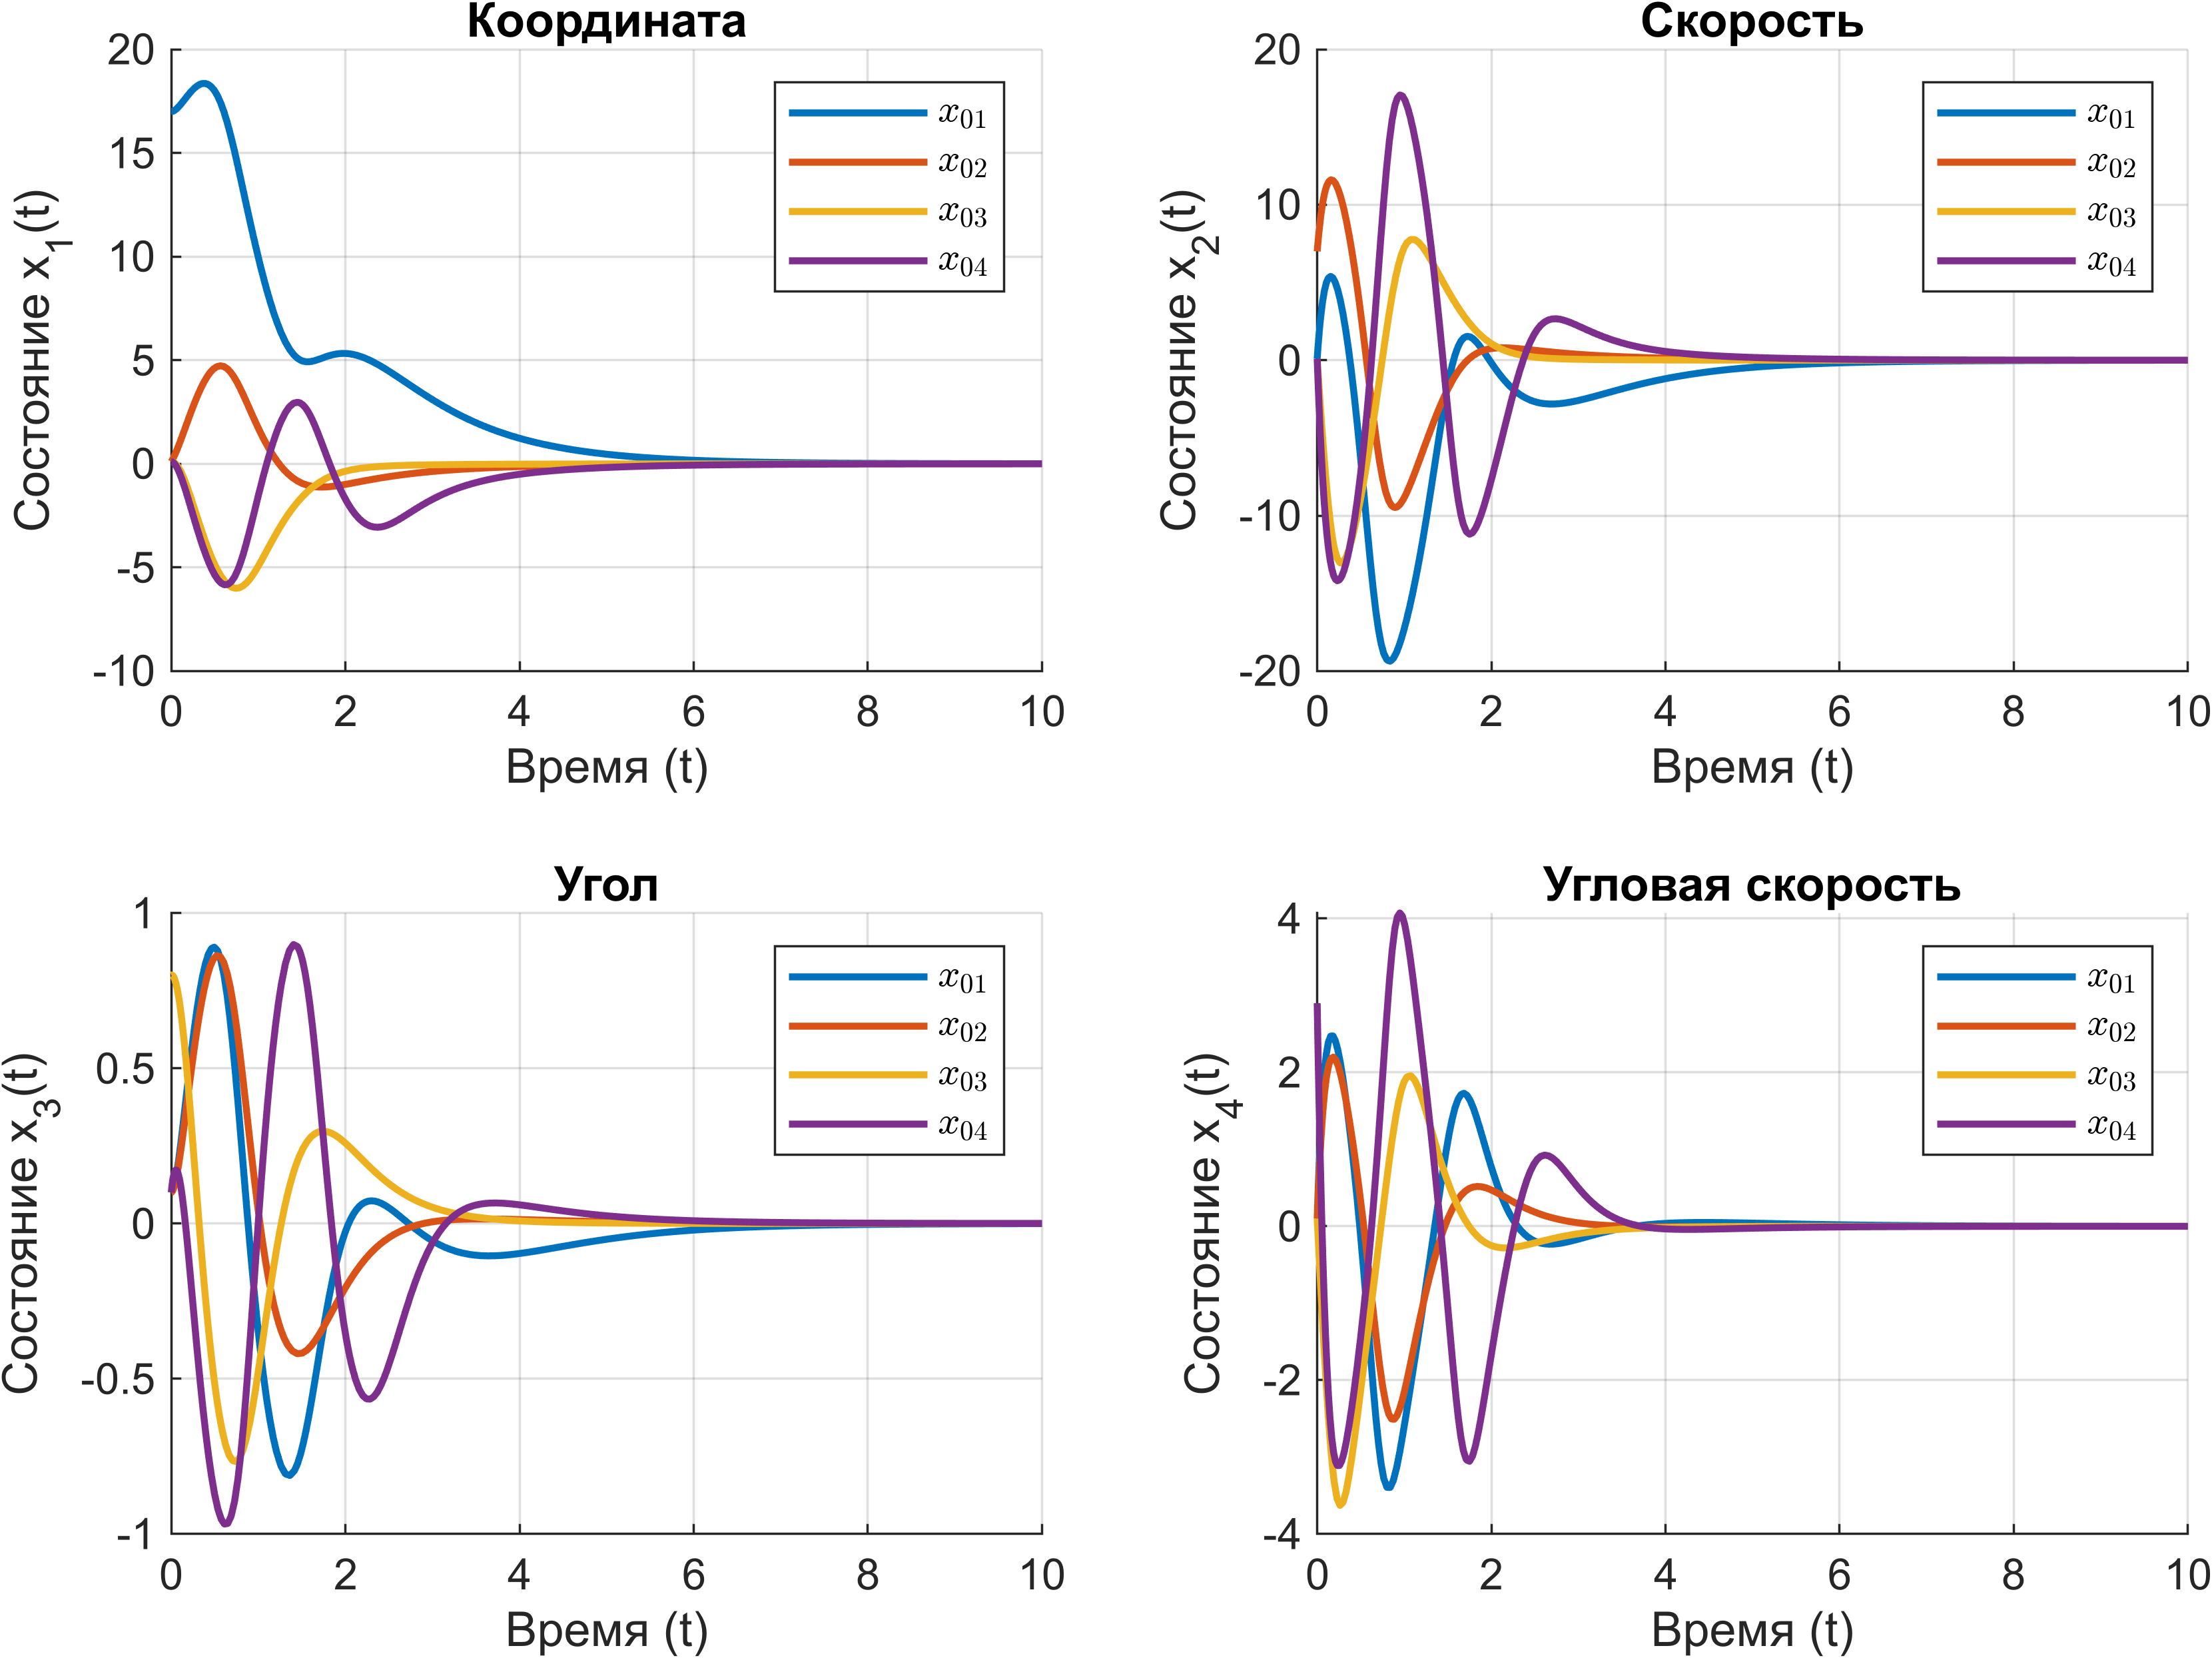
\includegraphics[width=\linewidth]{figs/3.1.good.png}
    \caption{Моделирование работы регулятора по состоянию с 
    устойчивыми начальными условиями}
    \label{fig:3.1.good}
\end{figure}

\noindent Рассмотрим еще 4 начальных условия:
\begin{equation*}
    x_{01}=\begin{bmatrix}
        40\\
        0.1\\
        0.1\\
        0.1
    \end{bmatrix},\quad
    x_{02}=\begin{bmatrix}
        0.1\\
         12\\
        0.1\\
         0.1
    \end{bmatrix},\quad
    x_{03}=\begin{bmatrix}
        0.1\\
         0.1\\
         1\\
         0.1
    \end{bmatrix},\quad
    x_{04}=\begin{bmatrix}
        0.1\\
         0.1\\
         0.1\\
         4
    \end{bmatrix},
\end{equation*}
при этих начальных условиях маятник падает. 
Графики состояния можно увидеть на \autoref{fig:3.1.badd}.
На 2 секунде, система достигла следующих состояний:
\begin{equation*}
    x_{01}(2)=\begin{bmatrix}
-4.1\cdot10^9 \\ -5.0\cdot10^{10} \\ 4.71 \\ 858.0
\end{bmatrix},\quad
    x_{02}(2)=\begin{bmatrix}
-6.8\cdot10^8 \\ -8.3\cdot10^9 \\ 4.72 \\ 1603.0
\end{bmatrix},\quad
    x_{03}(2)=\begin{bmatrix}
5.2\cdot10^7 \\ 6.4\cdot10^8 \\ -4.67 \\ 336.5
\end{bmatrix},\quad
    x_{04}(2)=\begin{bmatrix}
7.3\cdot10^6 \\ 9.0\cdot10^7 \\ 1.61 \\ 1152.0
\end{bmatrix},
\end{equation*}
соответственно для первого, второго, третьего и четвертого начальных условий.
Можно заметить, что система во всех случаях сводит угол маятника к $\pm90^\circ$.

\begin{figure}[H]
    \centering
    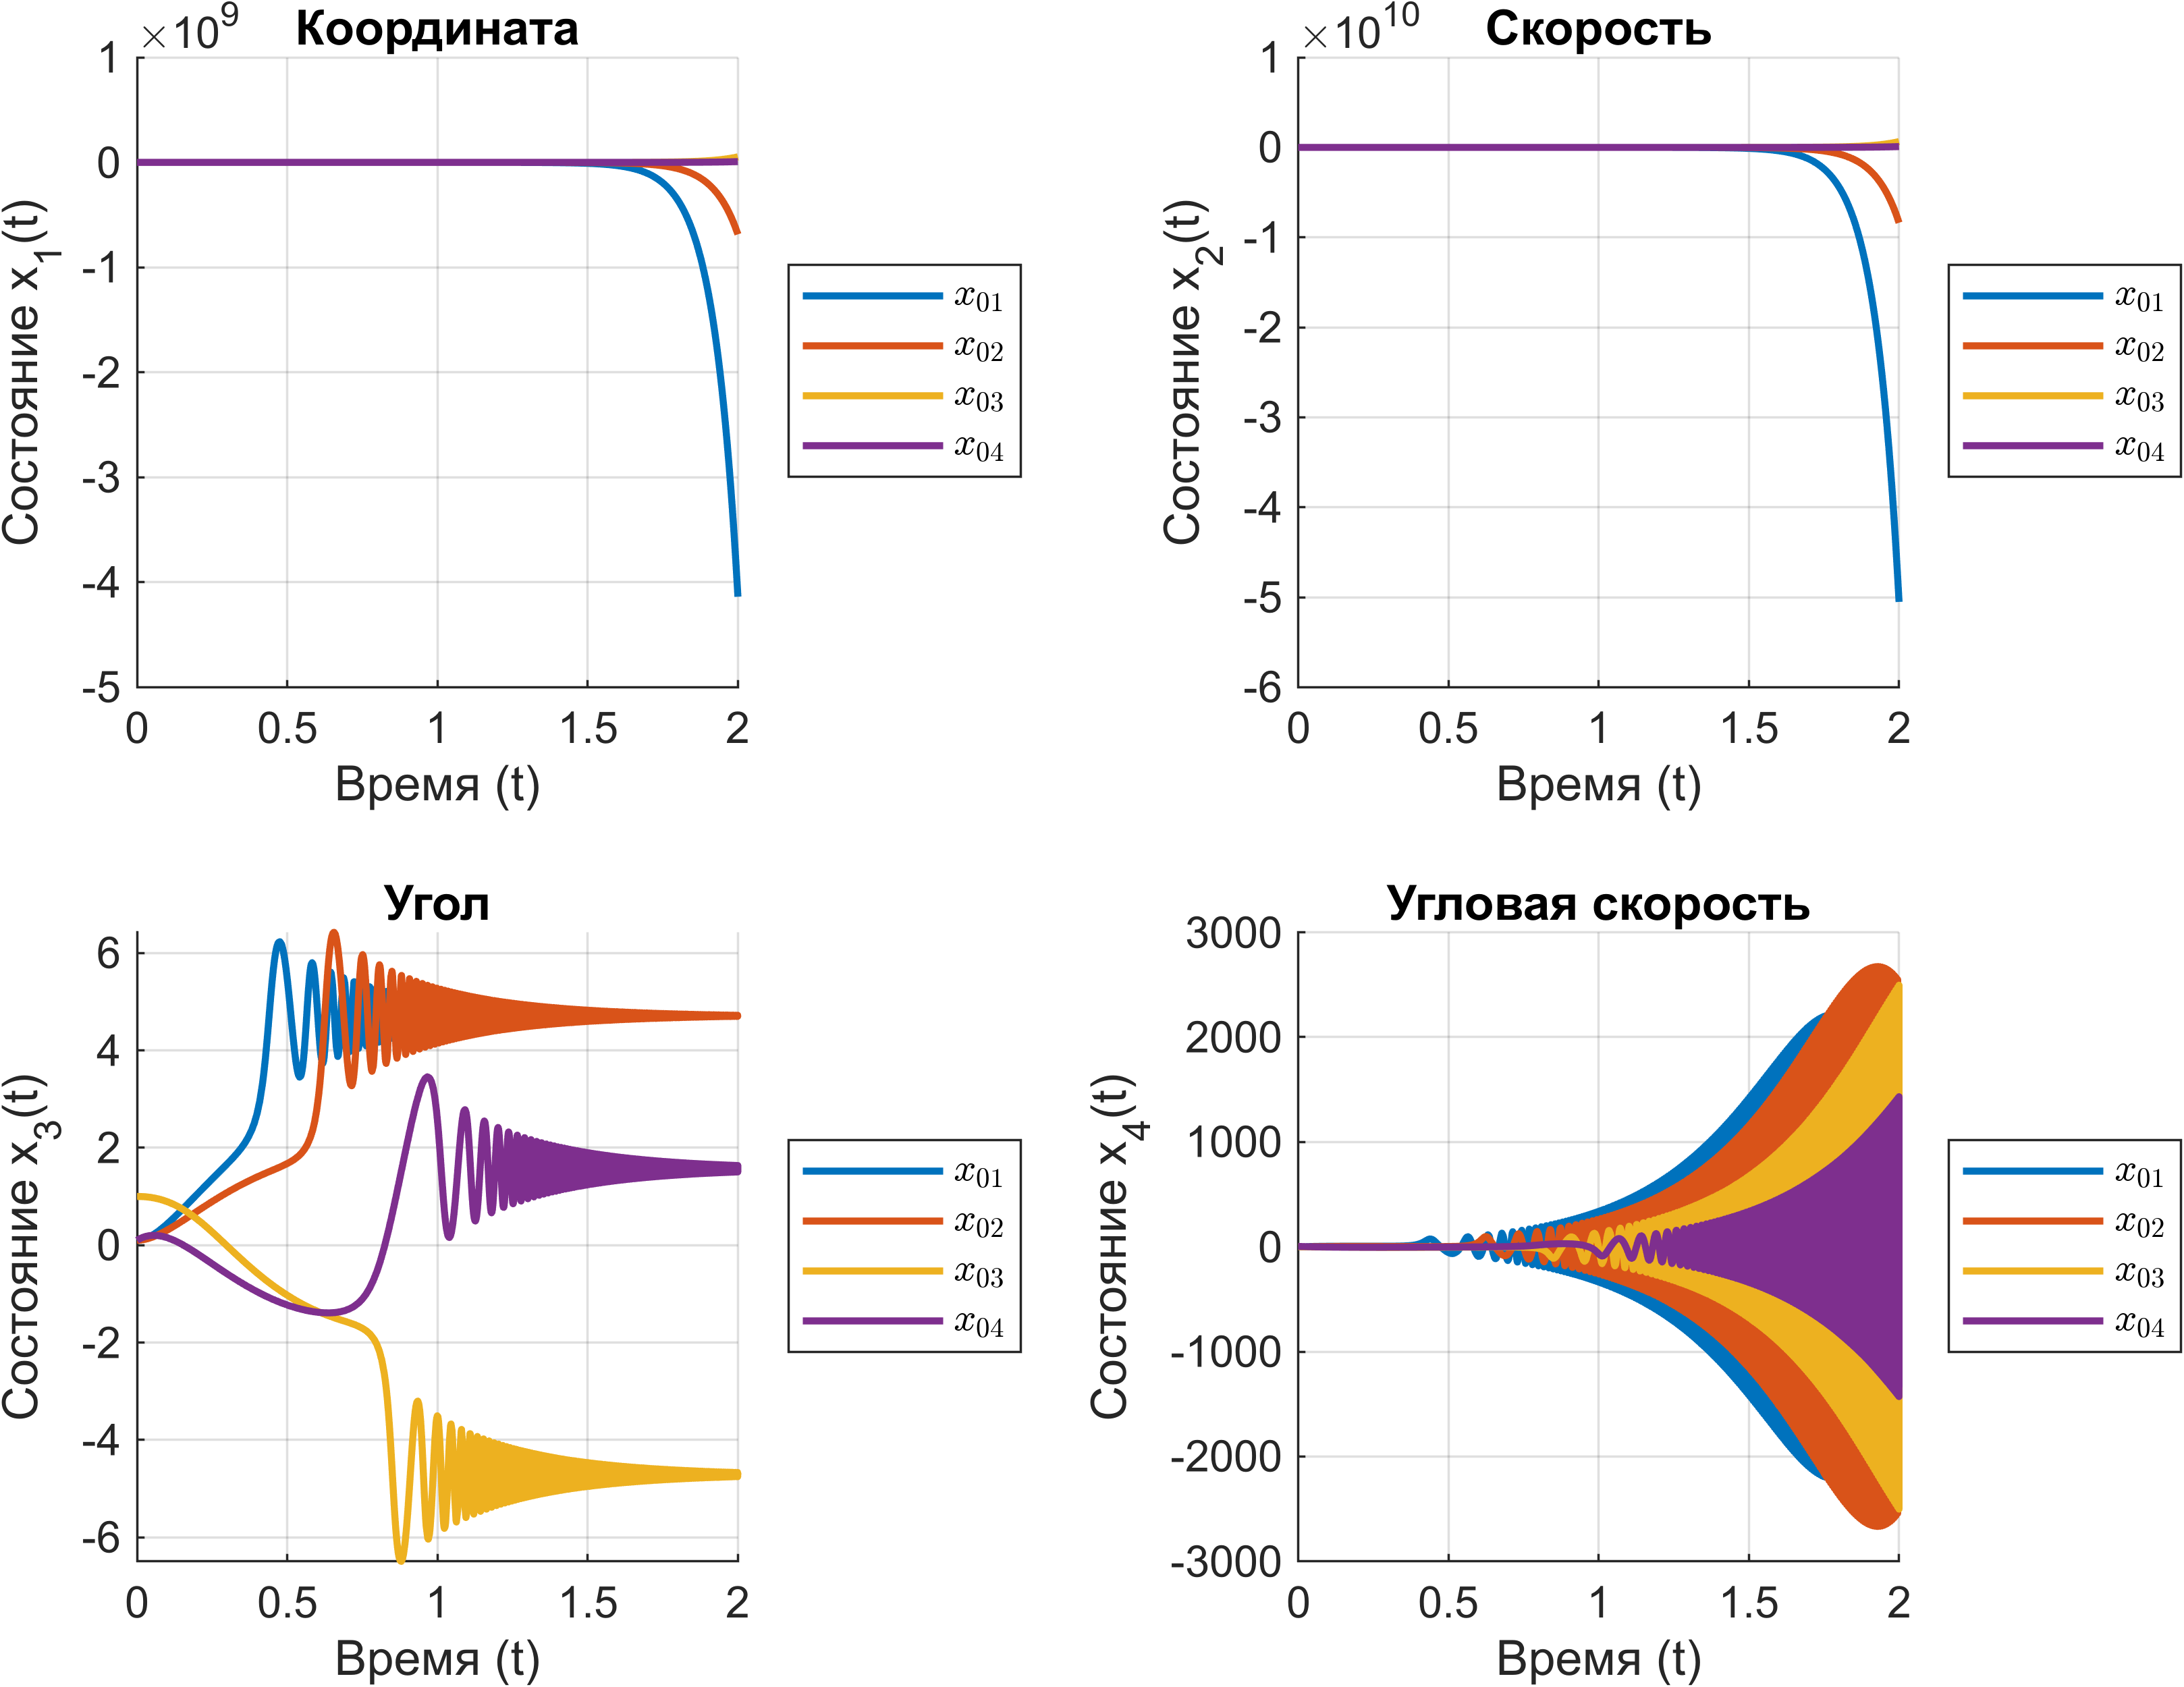
\includegraphics[width=\linewidth]{figs/3.1.badd.png}
    \caption{Моделирование работы регулятора по состоянию с 
    неустойчивыми начальными условиями}
    \label{fig:3.1.badd}
\end{figure}

\section{Исследование регулятора по состоянию}
\label{sec:3.2}
Исследуем влияние спектра замкнутой системы на максимальное отклонение 
маятника от вертикали, максимальное горизонтальное смещение тележки и 
максимальное значение управляющего сигнала
при управлении нелинейной системой \eqref{eq:origsys}.
Выберем начальное состояние, где все числа $0.1$, и пять спектров для
синтеза регуляторов:
\begin{gather*}
    \sigma_1=\left\{ \begin{array}{cccc}
        -1&-2&-3&-4
    \end{array} \right\},\\
    \sigma_2=\left\{ \begin{array}{cccc}
        -11&-2&-3&-4
    \end{array} \right\},\\
    \sigma_3=\left\{ \begin{array}{cccc}
        -11&-12&-3&-4
    \end{array} \right\},\\
    \sigma_4=\left\{ \begin{array}{cccc}
        -11&-12&-13&-4
    \end{array} \right\},\\
    \sigma_5=\left\{ \begin{array}{cccc}
        -11&-12&-13&-6
    \end{array} \right\},
\end{gather*}
и получим следующие матрицы регуляторов:
\begin{gather*}
    K_1=\begin{bmatrix}
        2793.0 & 5819.0 & -51340.0 & -25000.0
    \end{bmatrix},\\
    K_2=\begin{bmatrix}
        30730.0 & 36080.0 & -219300.0 & -107000.0
    \end{bmatrix},\\
    K_3=\begin{bmatrix}
        184400.0 & 139700.0 & -783300.0 & -360100.0
    \end{bmatrix},\\
    K_4=\begin{bmatrix}
        798900.0 & 400400.0 & -2525000.0 & -979900.0
    \end{bmatrix},\\
    K_5=\begin{bmatrix}
        1198000.0 & 500700.0 & -3540000.0 & -1216000.0
    \end{bmatrix}.
\end{gather*}
Желаемые спектры замкнутых систем успешно получились.
Графики симуляций можно увидеть на \autoref{fig:3.2.sim}. 
Как видно, чем собсвенные числа больше,
тем система сильнее колеблется и быстрее сходится. При первых 
двух матрицах угол отклонения маятника не уходили дальше 
начальных условий,ьпри $K_4$ максимальное отклонение тележки составило 
$0.67$ м, а при $K_5$ - $0.76$ м
и максимально отклонение маятника $0.24$ радиан или $13.8^\circ$ 
(стартовый угол был 5.7$^\circ$
во всех случах).

\begin{figure}[H]
    \centering
    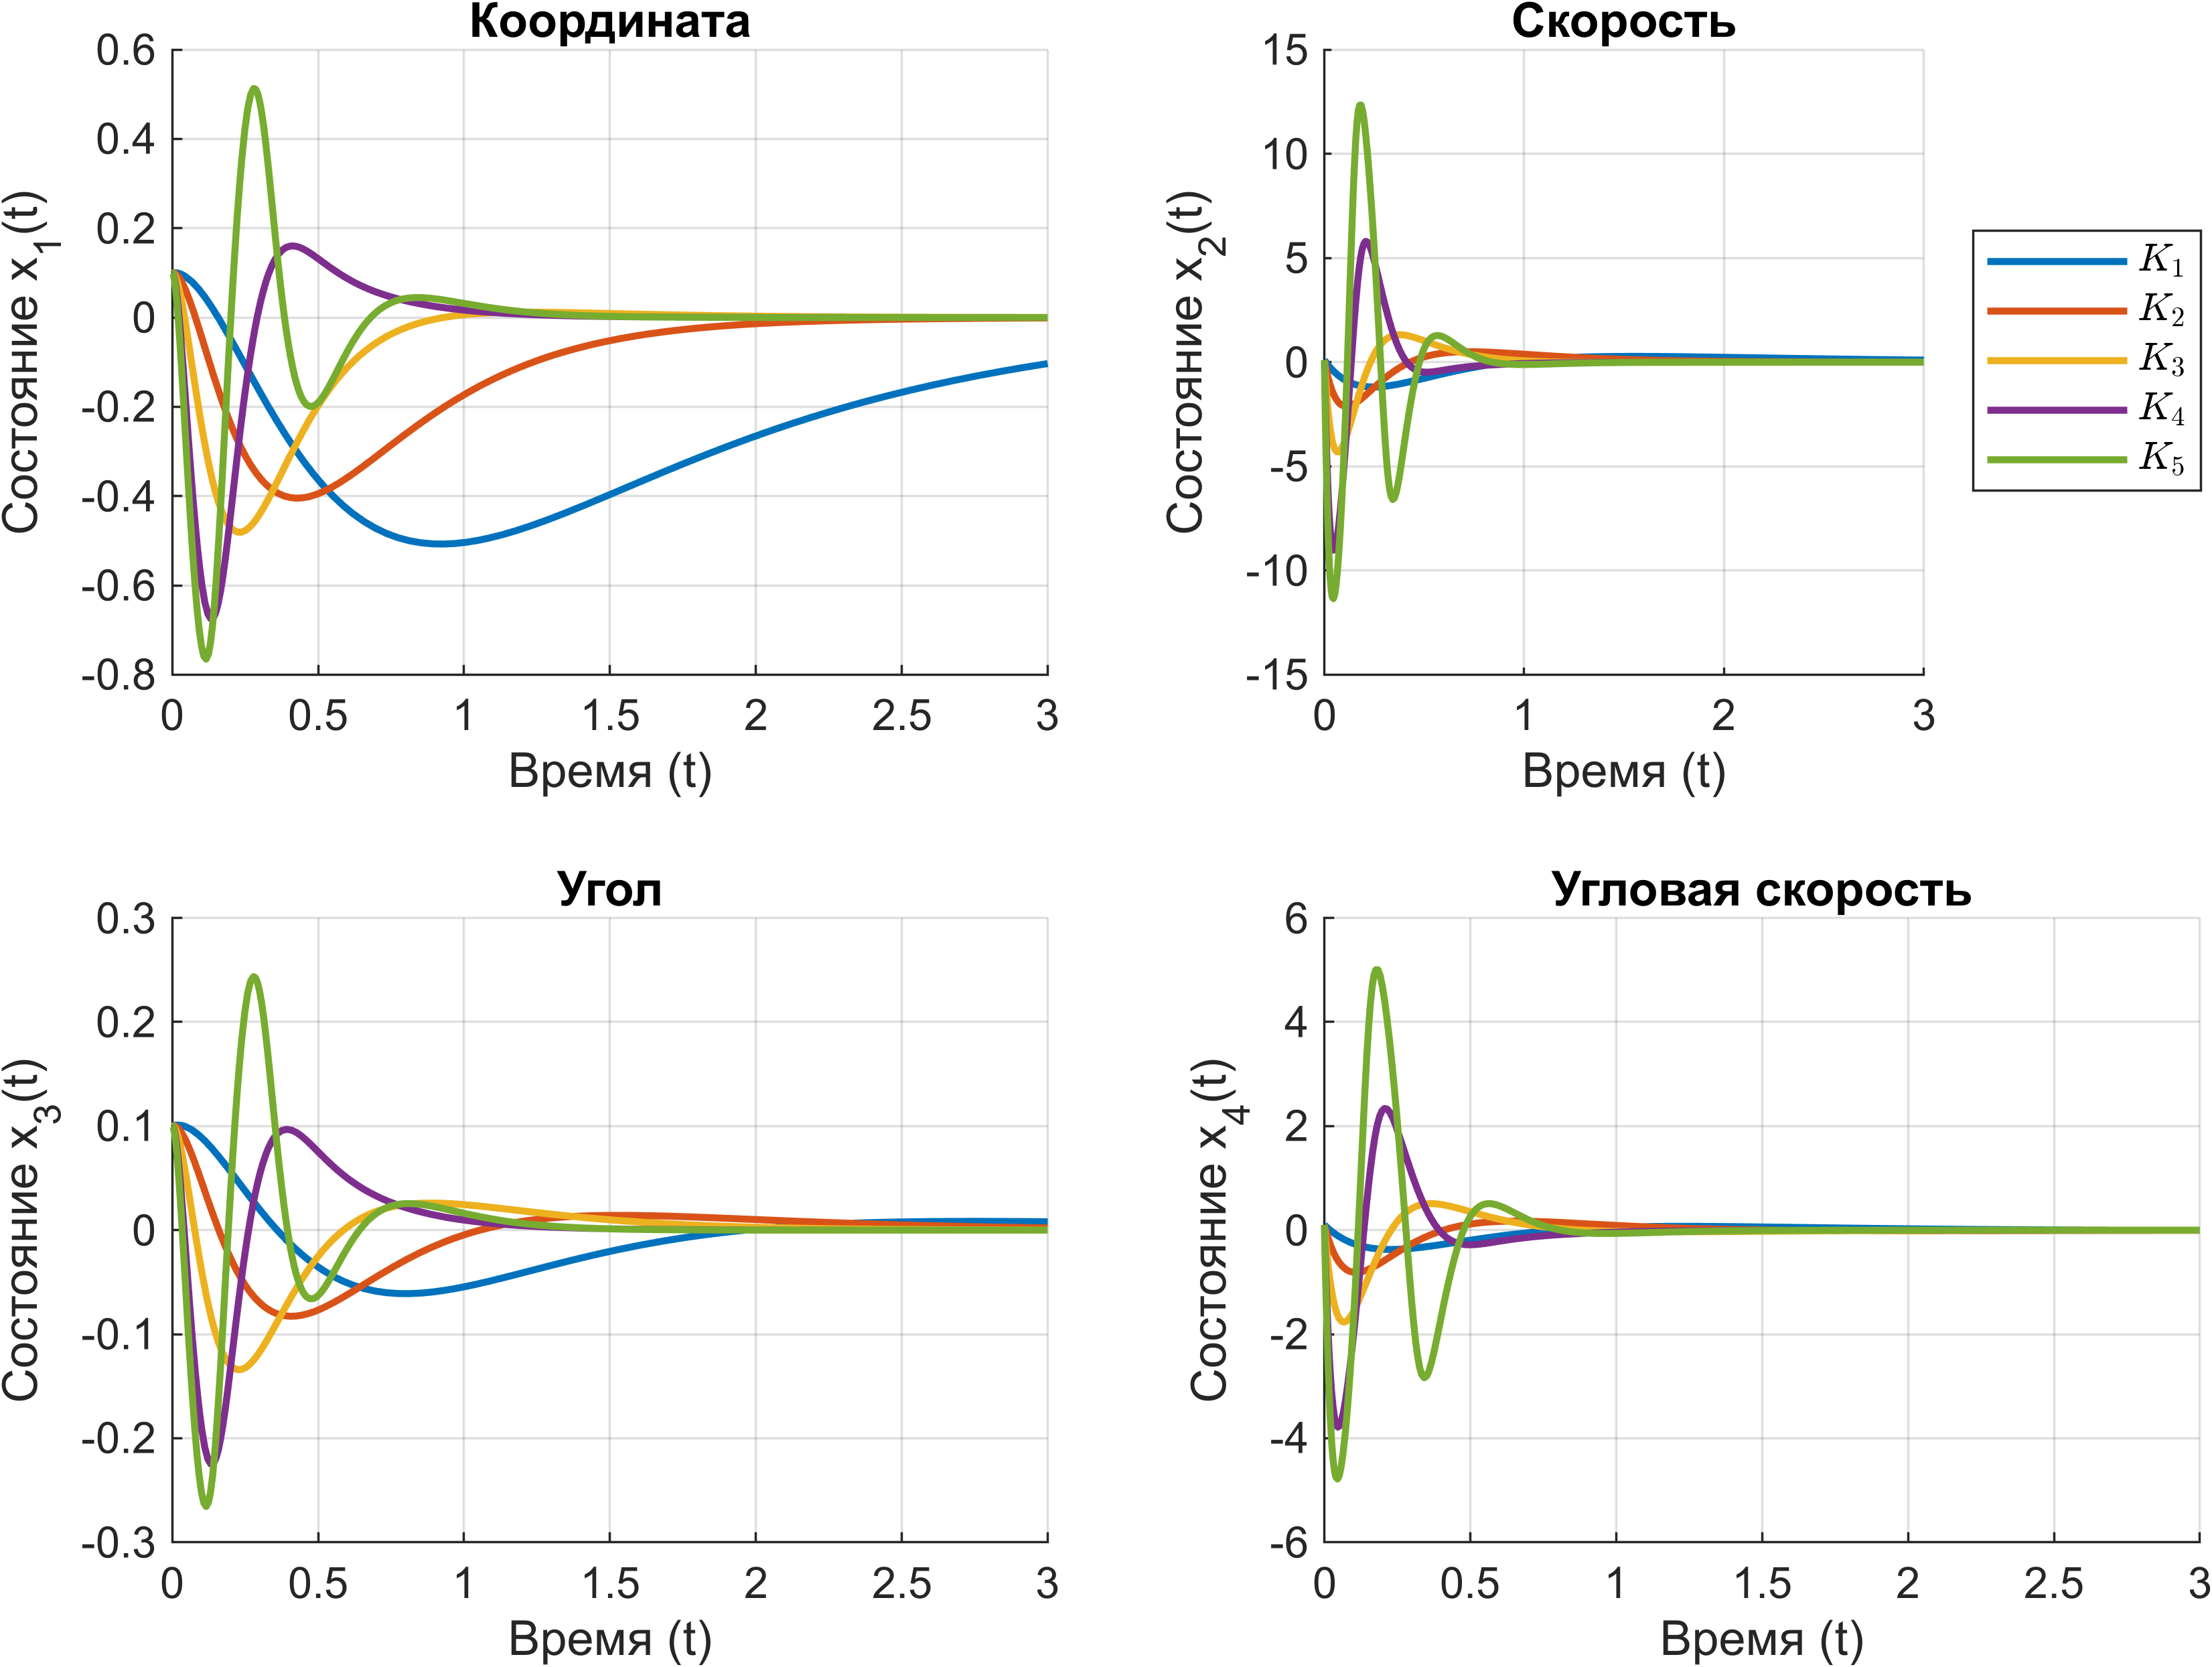
\includegraphics[width=\linewidth]{figs/3.2.sim.png}
    \caption{Моделирование работы регулятора по состоянию при
    рахных спектрах замкнутой системы}
    \label{fig:3.2.sim}
\end{figure}

\noindent Максимальное управление при каждом регуляторе можно увидеть на \autoref{fig:3.2.sim_u}.
Хотя собственные числа постепенно 
увеличивались на 10 поочередно (а при $K_5$ так вообще на 2), управление росло
не пропорцирнаоно, оно невероятно быстро увеличивается 
с увеличением значений собственных чисел.

\begin{figure}[H]
    \centering
    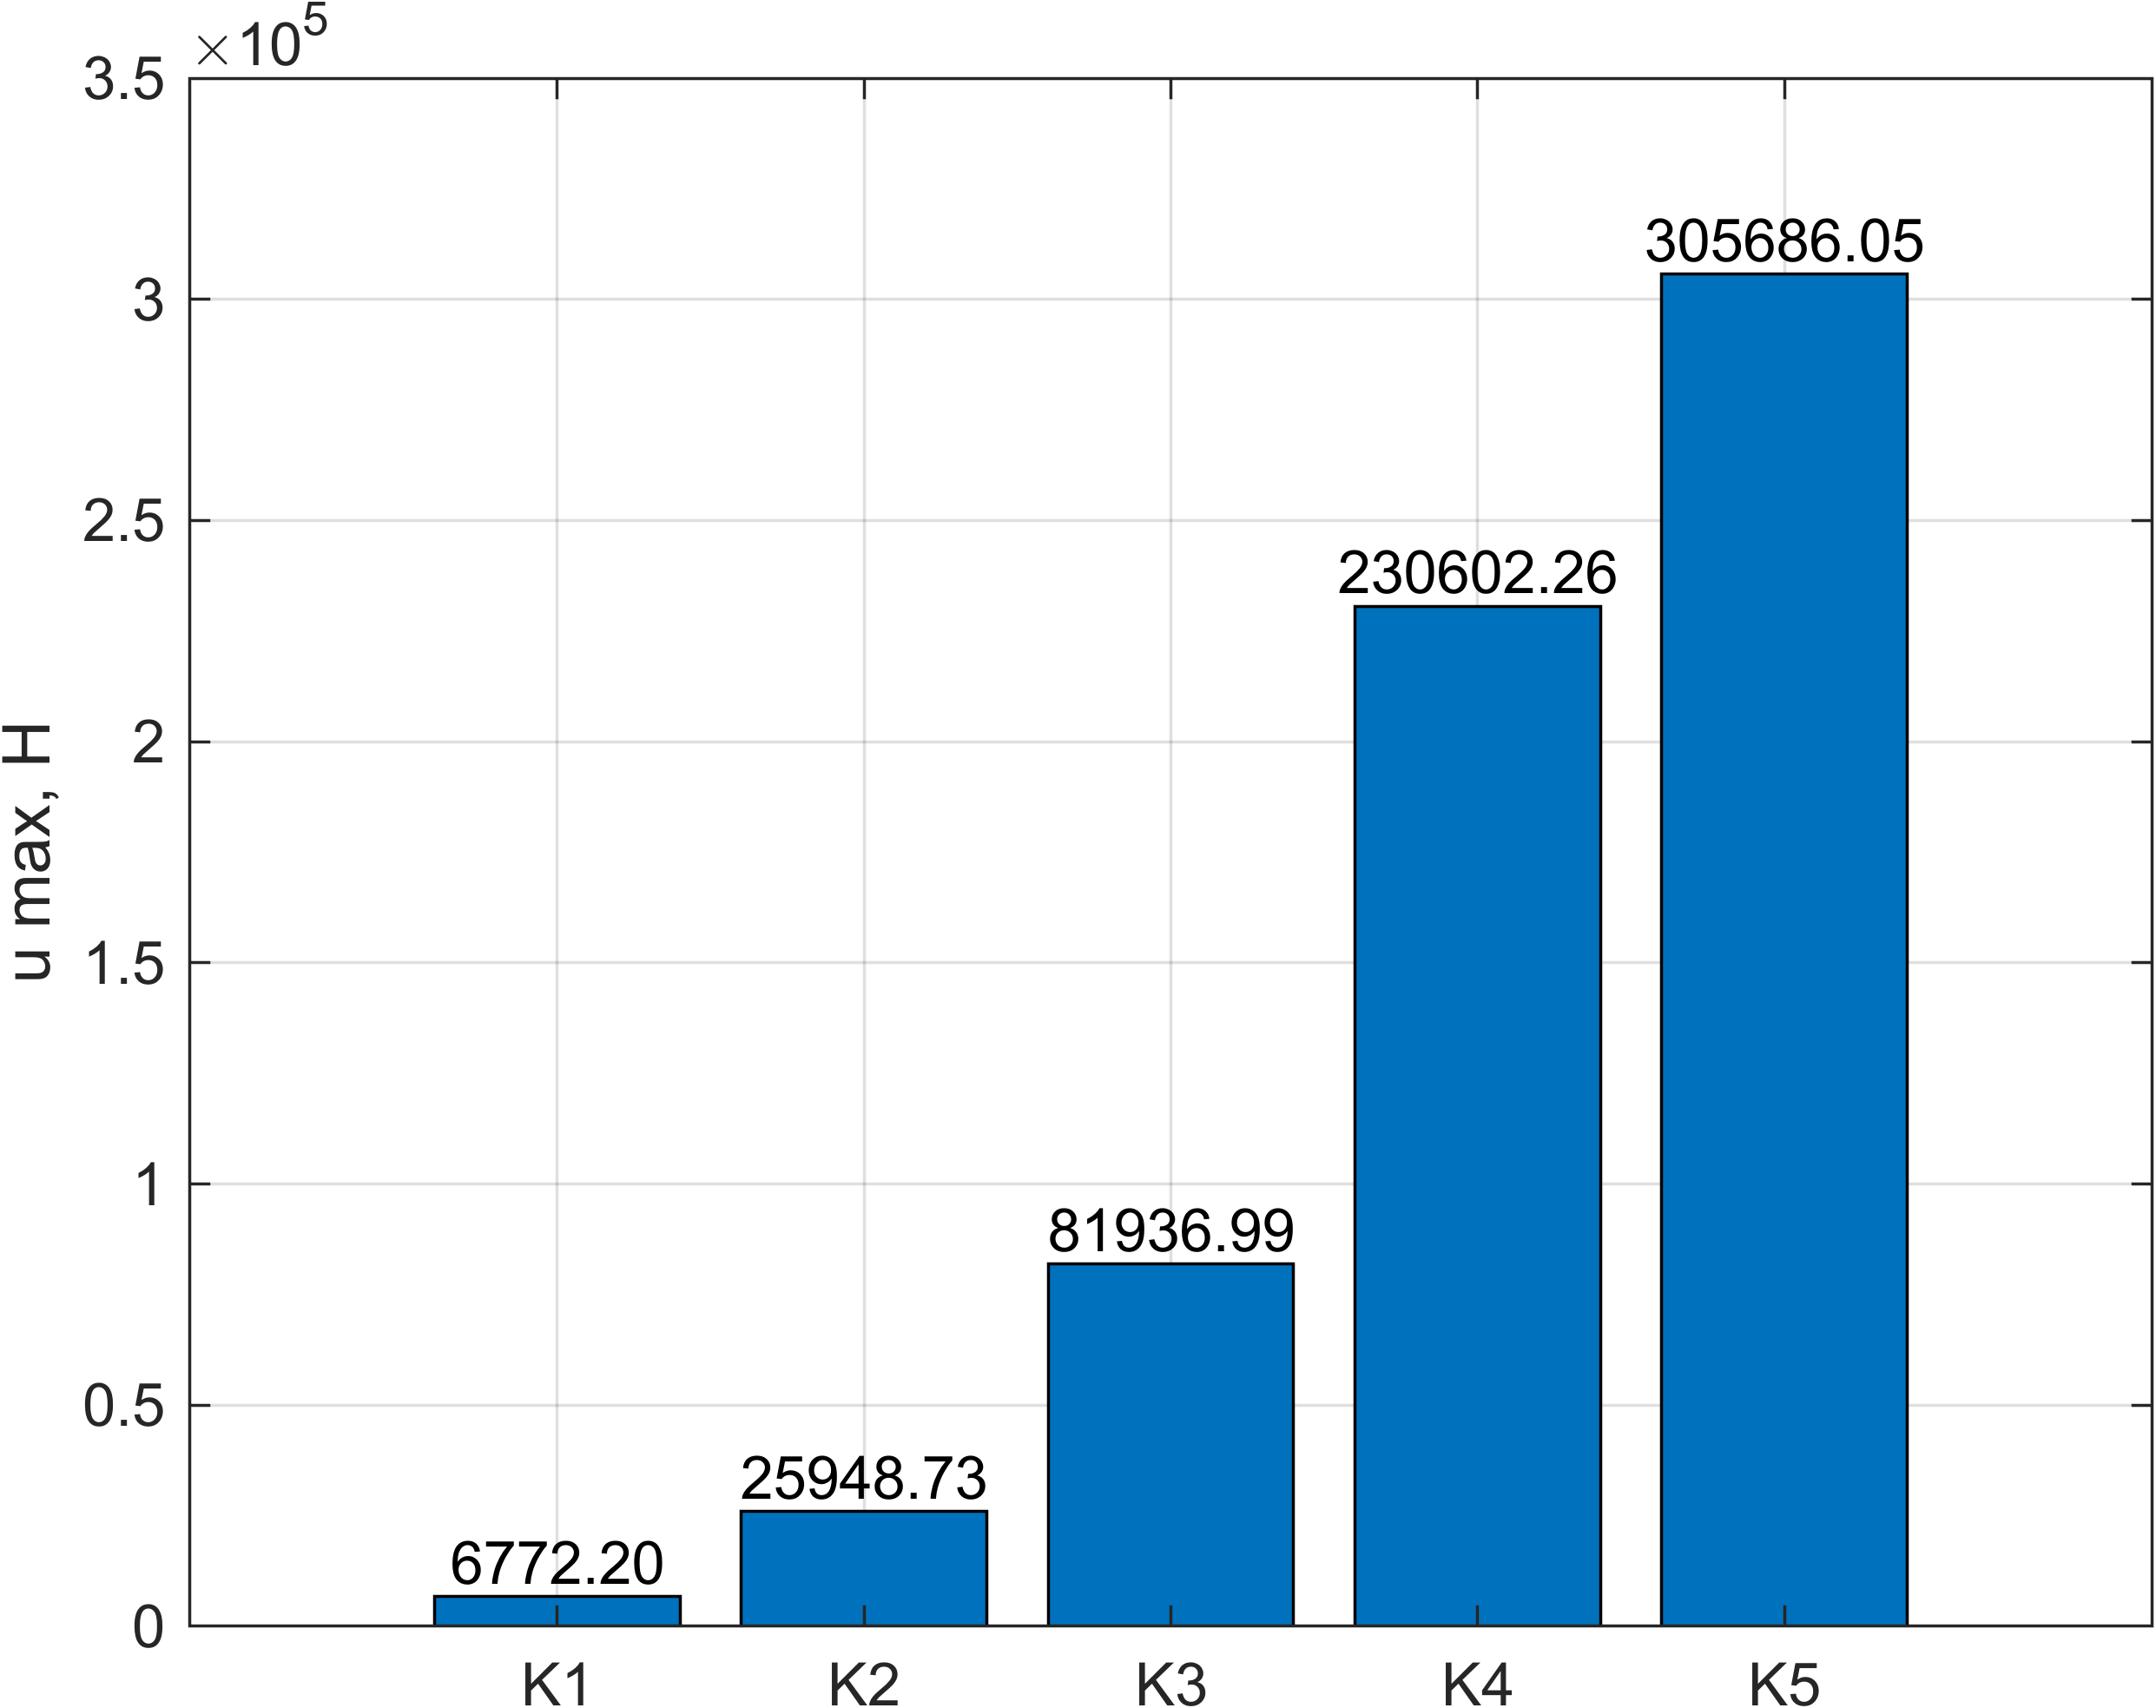
\includegraphics[width=\linewidth]{figs/3.2.sim_u.png}
    \caption{Максимальное управление}
    \label{fig:3.2.sim_u}
\end{figure}

\section{Синтез наблюдателя}

\subsection{Наблюдателя полного порядка}

Синтезируем наблюдателя полного порядка:
\begin{equation}
    \label{eq:3.3.estfull}
    \begin{cases}
        \dot{\hat x}=A\hat x+Bu+L(\hat y-y),\\
        \hat y=C\hat x.
    \end{cases}
\end{equation}
Для этого найдем решение уравнения Сильвестра:
\begin{equation*}
    \Gamma Q-QA=YC,\quad L=Q^{-1}Y,
\end{equation*}
возьмем следующие спектры ошибки наблюдателя:
\begin{gather*}
    \sigma_1=\left\{ \begin{array}{cccc}
        -1&-2&-3&-4
    \end{array} \right\},\\
    \sigma_2=\left\{ \begin{array}{cccc}
        -11&-2&-3&-4
    \end{array} \right\},\\
    \sigma_3=\left\{ \begin{array}{cccc}
        -11&-12&-3&-4
    \end{array} \right\},\\
    \sigma_4=\left\{ \begin{array}{cccc}
        -11&-12&-13&-4
    \end{array} \right\},\\
    \sigma_5=\left\{ \begin{array}{cccc}
        -11&-12&-13&-14
    \end{array} \right\},
\end{gather*}
и получим следующие матрицы наблюдателя:
\begin{gather*}
    L_1=\begin{bmatrix}
        11.14 & 11.14\\
        4.386 & 4.386\\
        -21.14 & -21.14\\
        -43.64 & -43.64
    \end{bmatrix},\quad
    L_2=\begin{bmatrix}
70.24 & 70.24\\
56.69 & 56.69\\
-90.24 & -90.24\\
-185.9 & -185.9
    \end{bmatrix},\quad
    L_3=\begin{bmatrix}
273.2 & 273.2\\
353.1 & 353.1\\
-303.2 & -303.2\\
-662.4 & -662.4
    \end{bmatrix},\\
    L_4=\begin{bmatrix}
784.5 & 784.5\\
1551.0 & 1551.0\\
-824.5 & -824.5\\
-2131.0 & -2131.0
    \end{bmatrix},\quad
    L_5=\begin{bmatrix}
1769.0 & 1769.0\\
5460.0 & 5460.0\\
-1819.0 & -1819.0\\
-6400.0 & -6400.0
    \end{bmatrix}.
\end{gather*}
Желаемые спектры ошибки наблюдателя успешно получились.
Для  дальнейших симуляций в качестве регулятора возьмем матрицу
$K_1$ из предыдущего пункта. 
Система будет начинать с состояния, где все числа $0.1$, а 
наблюдатель из нулевого состояния.
Графики симуляций можно увидеть на 
\autoref{fig:3.3.full}. Как видно, чем собственные числа наблюдателя больше,
тем система сильнее колеблется и быстрее сходится, кроме скорости,
она быстрее всего сходится при наименьшем значении собственных чисел.

\begin{figure}[H]
    \centering
    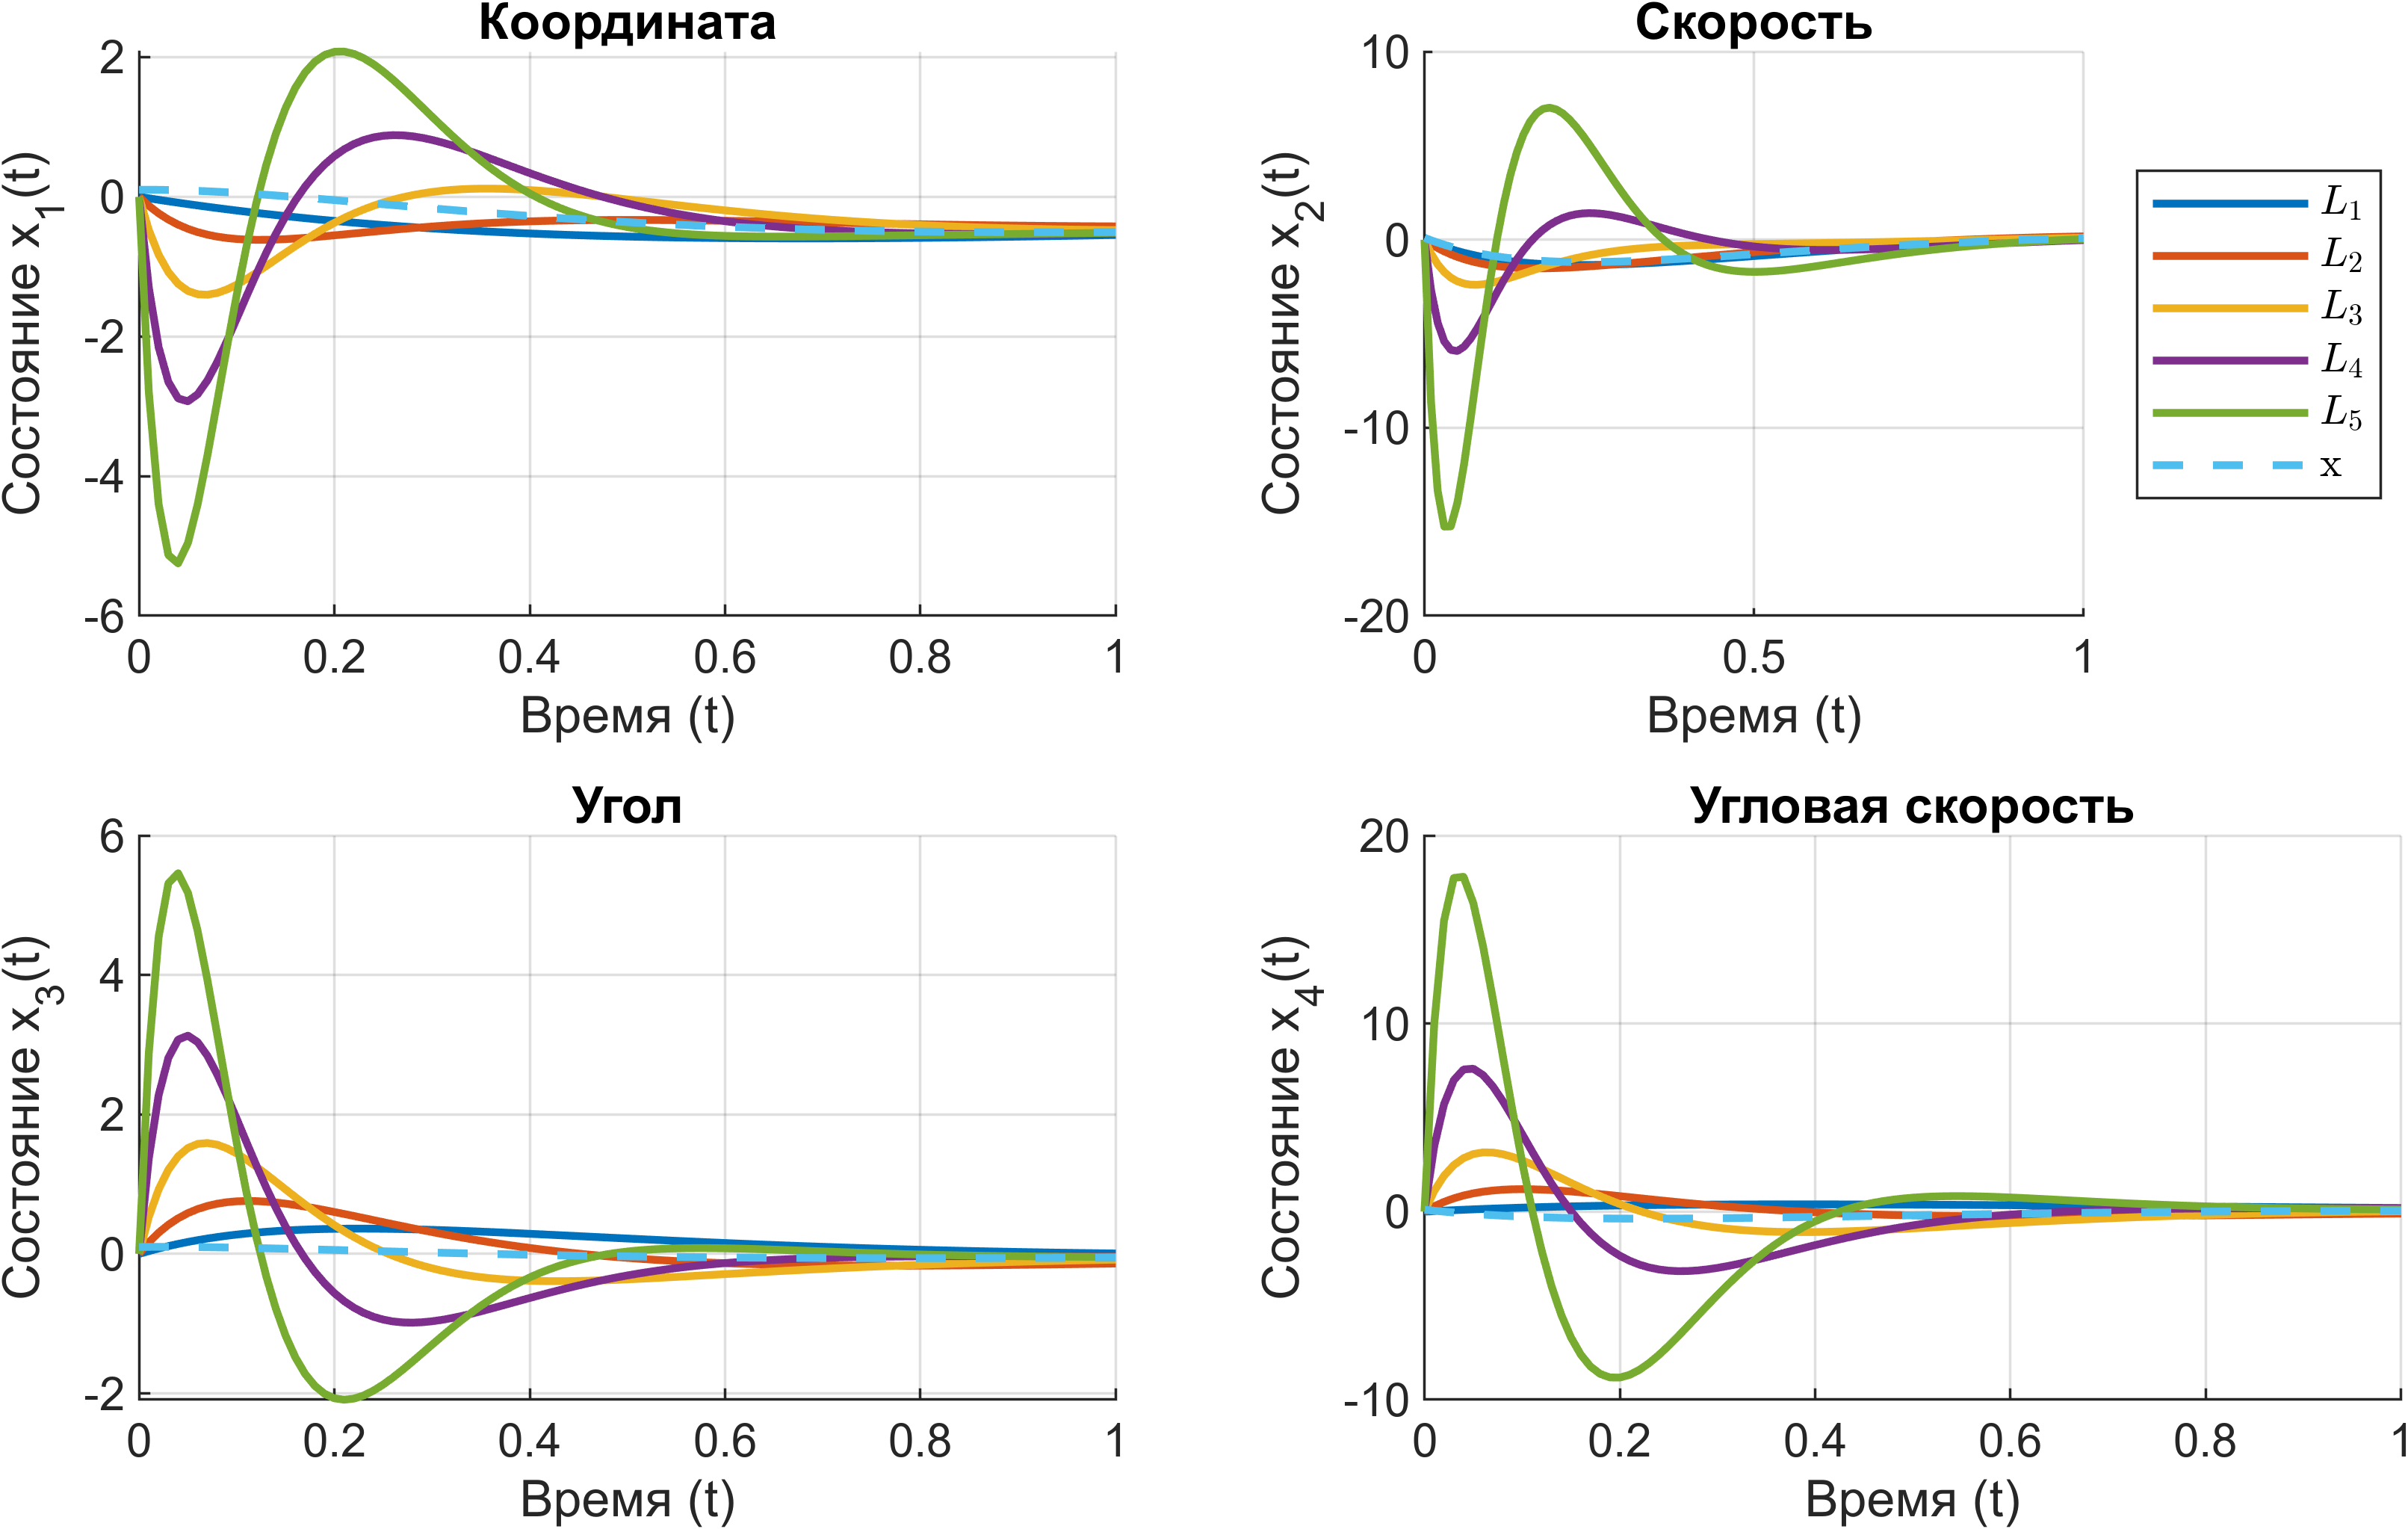
\includegraphics[width=\linewidth]{figs/3.3.full.png}
    \caption{Моделирование работы регулятора по состоянию 
    с наблюдателем полного порядка}
    \label{fig:3.3.full}
\end{figure}

\subsection{Наблюдатель пониженного порядка}
\label{sec:3.3.red}

Синтезируем наблюдателя полного порядка:
\begin{equation}
    \label{eq:3.3.estred}
    \dot{\hat z}=\Gamma z-Yy+QBu,\quad \hat x=\begin{bmatrix}
        C\\Q
    \end{bmatrix}^{-1}\cdot\begin{bmatrix}
        y\\\hat z
    \end{bmatrix}.
\end{equation}
Для этого найдем решение уравнения Сильвестра:
\begin{equation*}
    \Gamma Q-QA=YC,
\end{equation*}
возьмем следующие спектры для матрицы $\Gamma$:
\begin{gather*}
    \sigma_1=\left\{ \begin{array}{cccc}
        -1&-2
    \end{array} \right\},\\
    \sigma_2=\left\{ \begin{array}{cccc}
        -6&-2
    \end{array} \right\},\\
    \sigma_3=\left\{ \begin{array}{cccc}
        -6&-4
    \end{array} \right\},
\end{gather*}
и получим следующие матрицы:
\begin{gather*}
    Q_1=\begin{bmatrix}
-1.0 & 1.0 & 0.3446 & -0.3446\\
-0.5 & 0.25 & 8.032 & -4.016
    \end{bmatrix},\\
    Q_2=\begin{bmatrix}
-0.1667 & 0.02778 & -0.1897 & 0.03161\\
-0.5 & 0.25 & 8.032 & -4.016
    \end{bmatrix},\\
    Q_3=\begin{bmatrix}
-0.1667 & 0.02778 & -0.1897 & 0.03161\\
-0.25 & 0.0625 & -0.3432 & 0.0858
    \end{bmatrix}.
\end{gather*}
Для  дальнейших симуляций в качестве регулятора возьмем матрицу
$K_1$ из предыдущего пункта. 
Система будет начинать с состояния, где все числа $0.1$, а 
наблюдатель из нулевого состояния.
Графики симуляций можно увидеть на 
\autoref{fig:3.3.reduced}. Как видно, оценка координаты и угла полностью совпадают
с настоящими, что ожидается от редуцированного наблюдателя.
Схоже с наблюдателем полного порядка, редуцированный, при увеличении собственных чисел,
все больше и больше ошибается в начальный момент времени, но, в отличии от него,
гораздо сильнее реагирует на увеличение собственных чисел.
Так же подмечу, что наблюдадель пониженного порядка быстрее сошелся, чем полный.
Таким образом, наблюдатель пониженного порядка предпочтительнее во всех аспектах.

\begin{figure}[H]
    \centering
    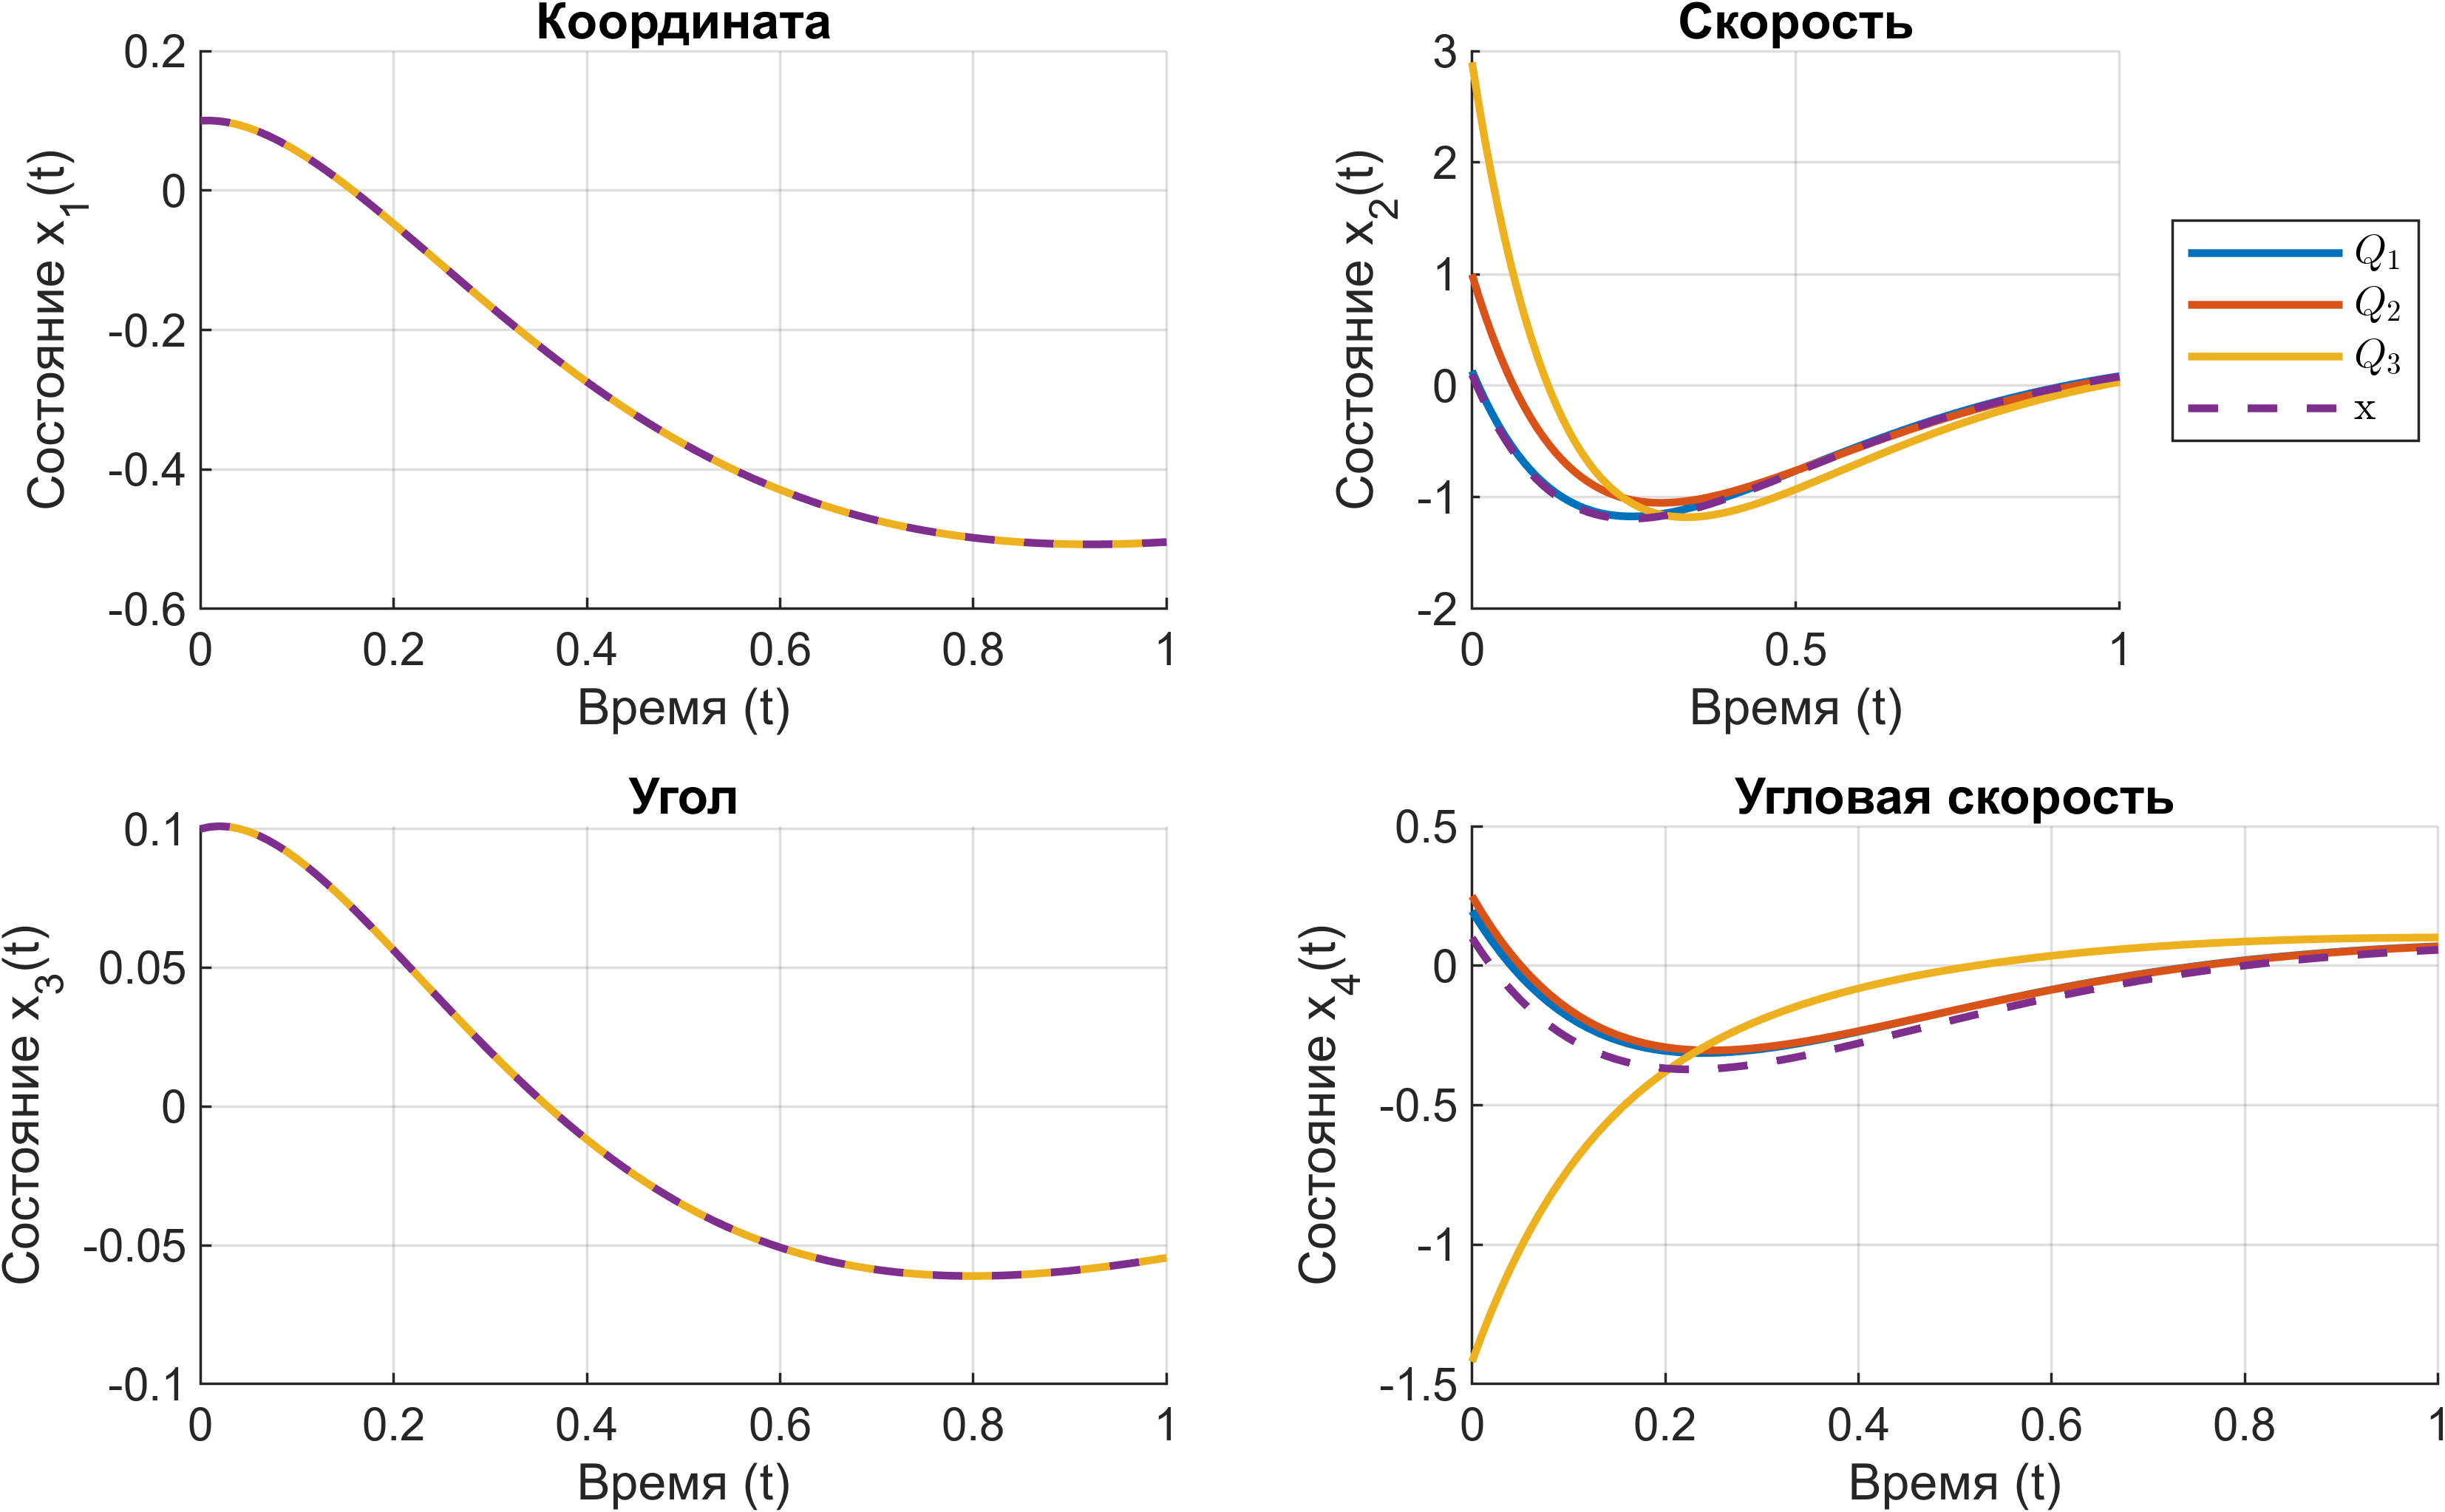
\includegraphics[width=\linewidth]{figs/3.3.reduced.png}
    \caption{Моделирование работы регулятора по состоянию 
    с наблюдателем пониженного порядка}
    \label{fig:3.3.reduced}
\end{figure}

\section{Синтез регулятора по выходу}

Построим регулятор, стабилизирующий маятник и тележку в условиях, 
когда измерению доступны только сигналы $y_1$ и $y_2$. Для
этого используем редуцированный наблюдатель из предыдущего пункта 
и, основанный на нем, закон управления
\begin{equation*}
    u=K\hat x.
\end{equation*}
Для начала просимулируем как себя ведет система с управлением по выходу и 
наблюдателями и пункта \autoref{sec:3.3.red}. Результат можно увидеть на
\autoref{fig:3.4.wat}. Как видно, система ведет абсолютно по другому, нежели при
управлении по состоянию, но наблюдаьель $Q_1$ все еще справляется лучше всех.
\begin{figure}[H]
    \centering
    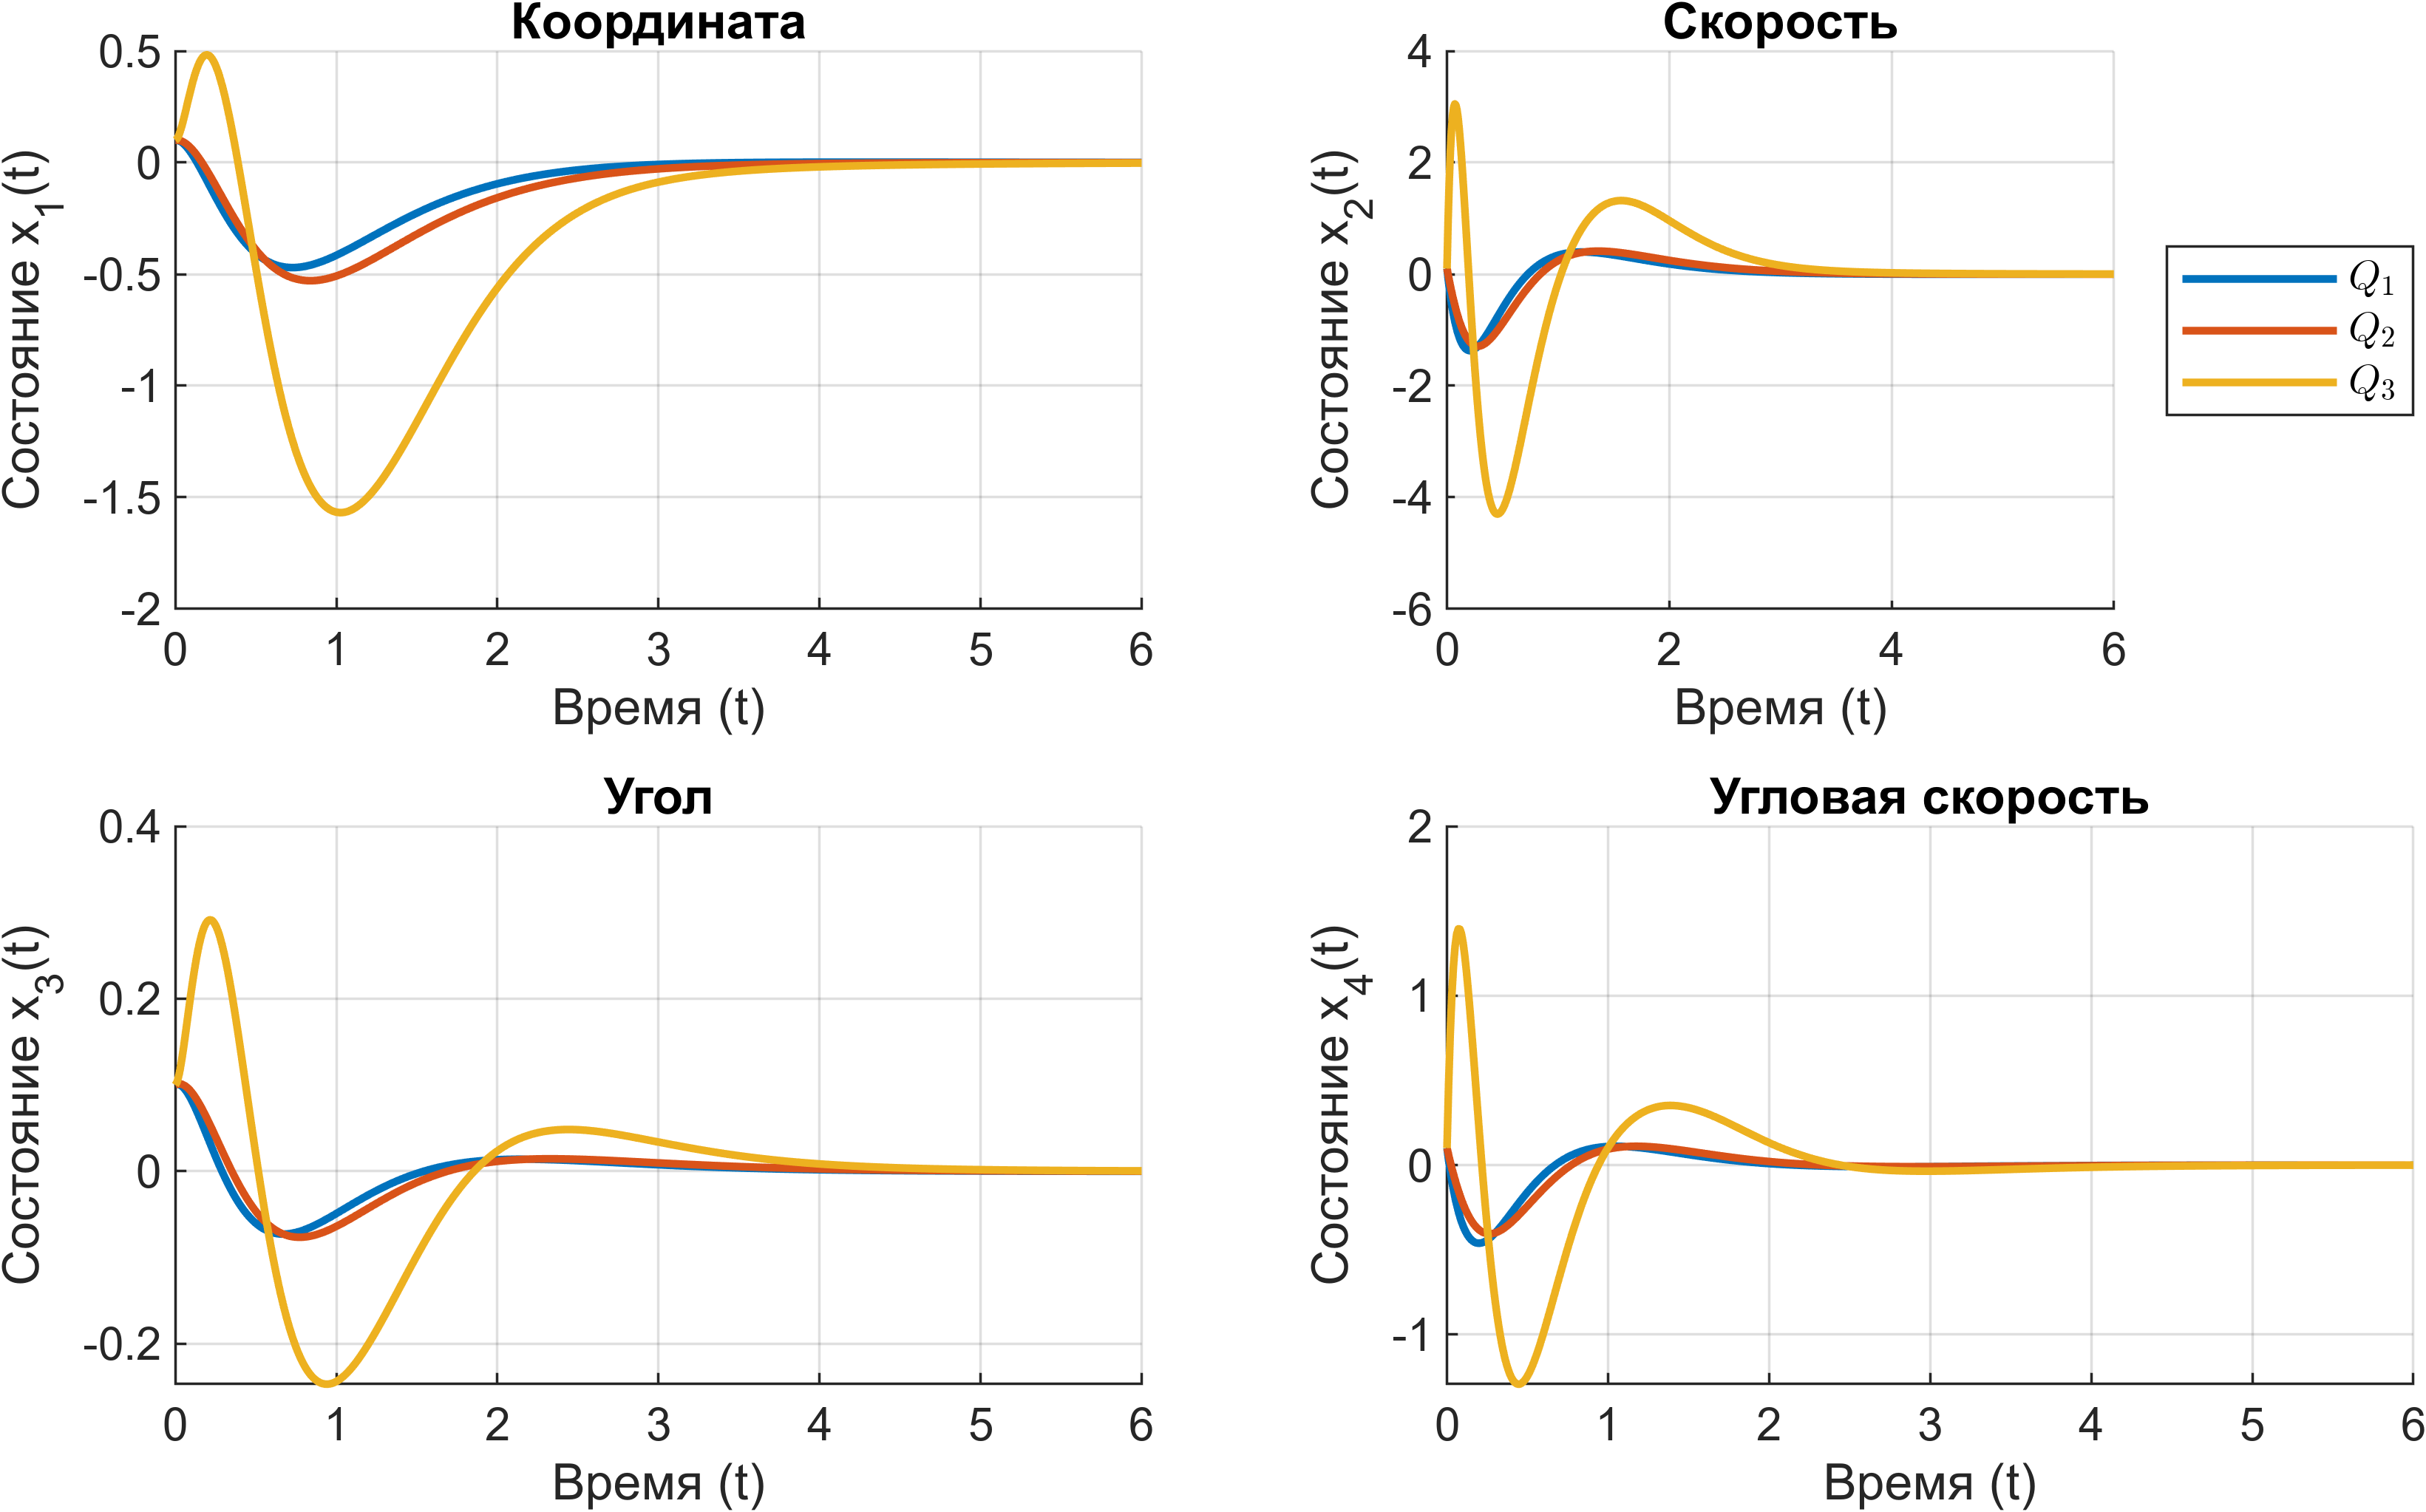
\includegraphics[width=\linewidth]{figs/3.4.wat.png}
    \caption{Моделирование работы регулятора по выходу 
    с наблюдателями пониженного порядка}
    \label{fig:3.4.wat}
\end{figure}
\noindent Теперь просимулируем как себя ведет система с управлением по выходу и
с наблюдателем пониженного порядка $Q_1$ и первыми тремя 
регуляторами из \autoref{sec:3.2}, рассмотрим только эти, потому что
затраты на упралвение у последних двух просто космические.
Симуляцию можно увидеть на \autoref{fig:3.4.watK}. Результаты ожидаемые, но
елси вспомнить управление, требуемое для данных регуляторов, то
я вижу единственным реалистичным вариантом $K_1$.
\begin{figure}[H]
    \centering
    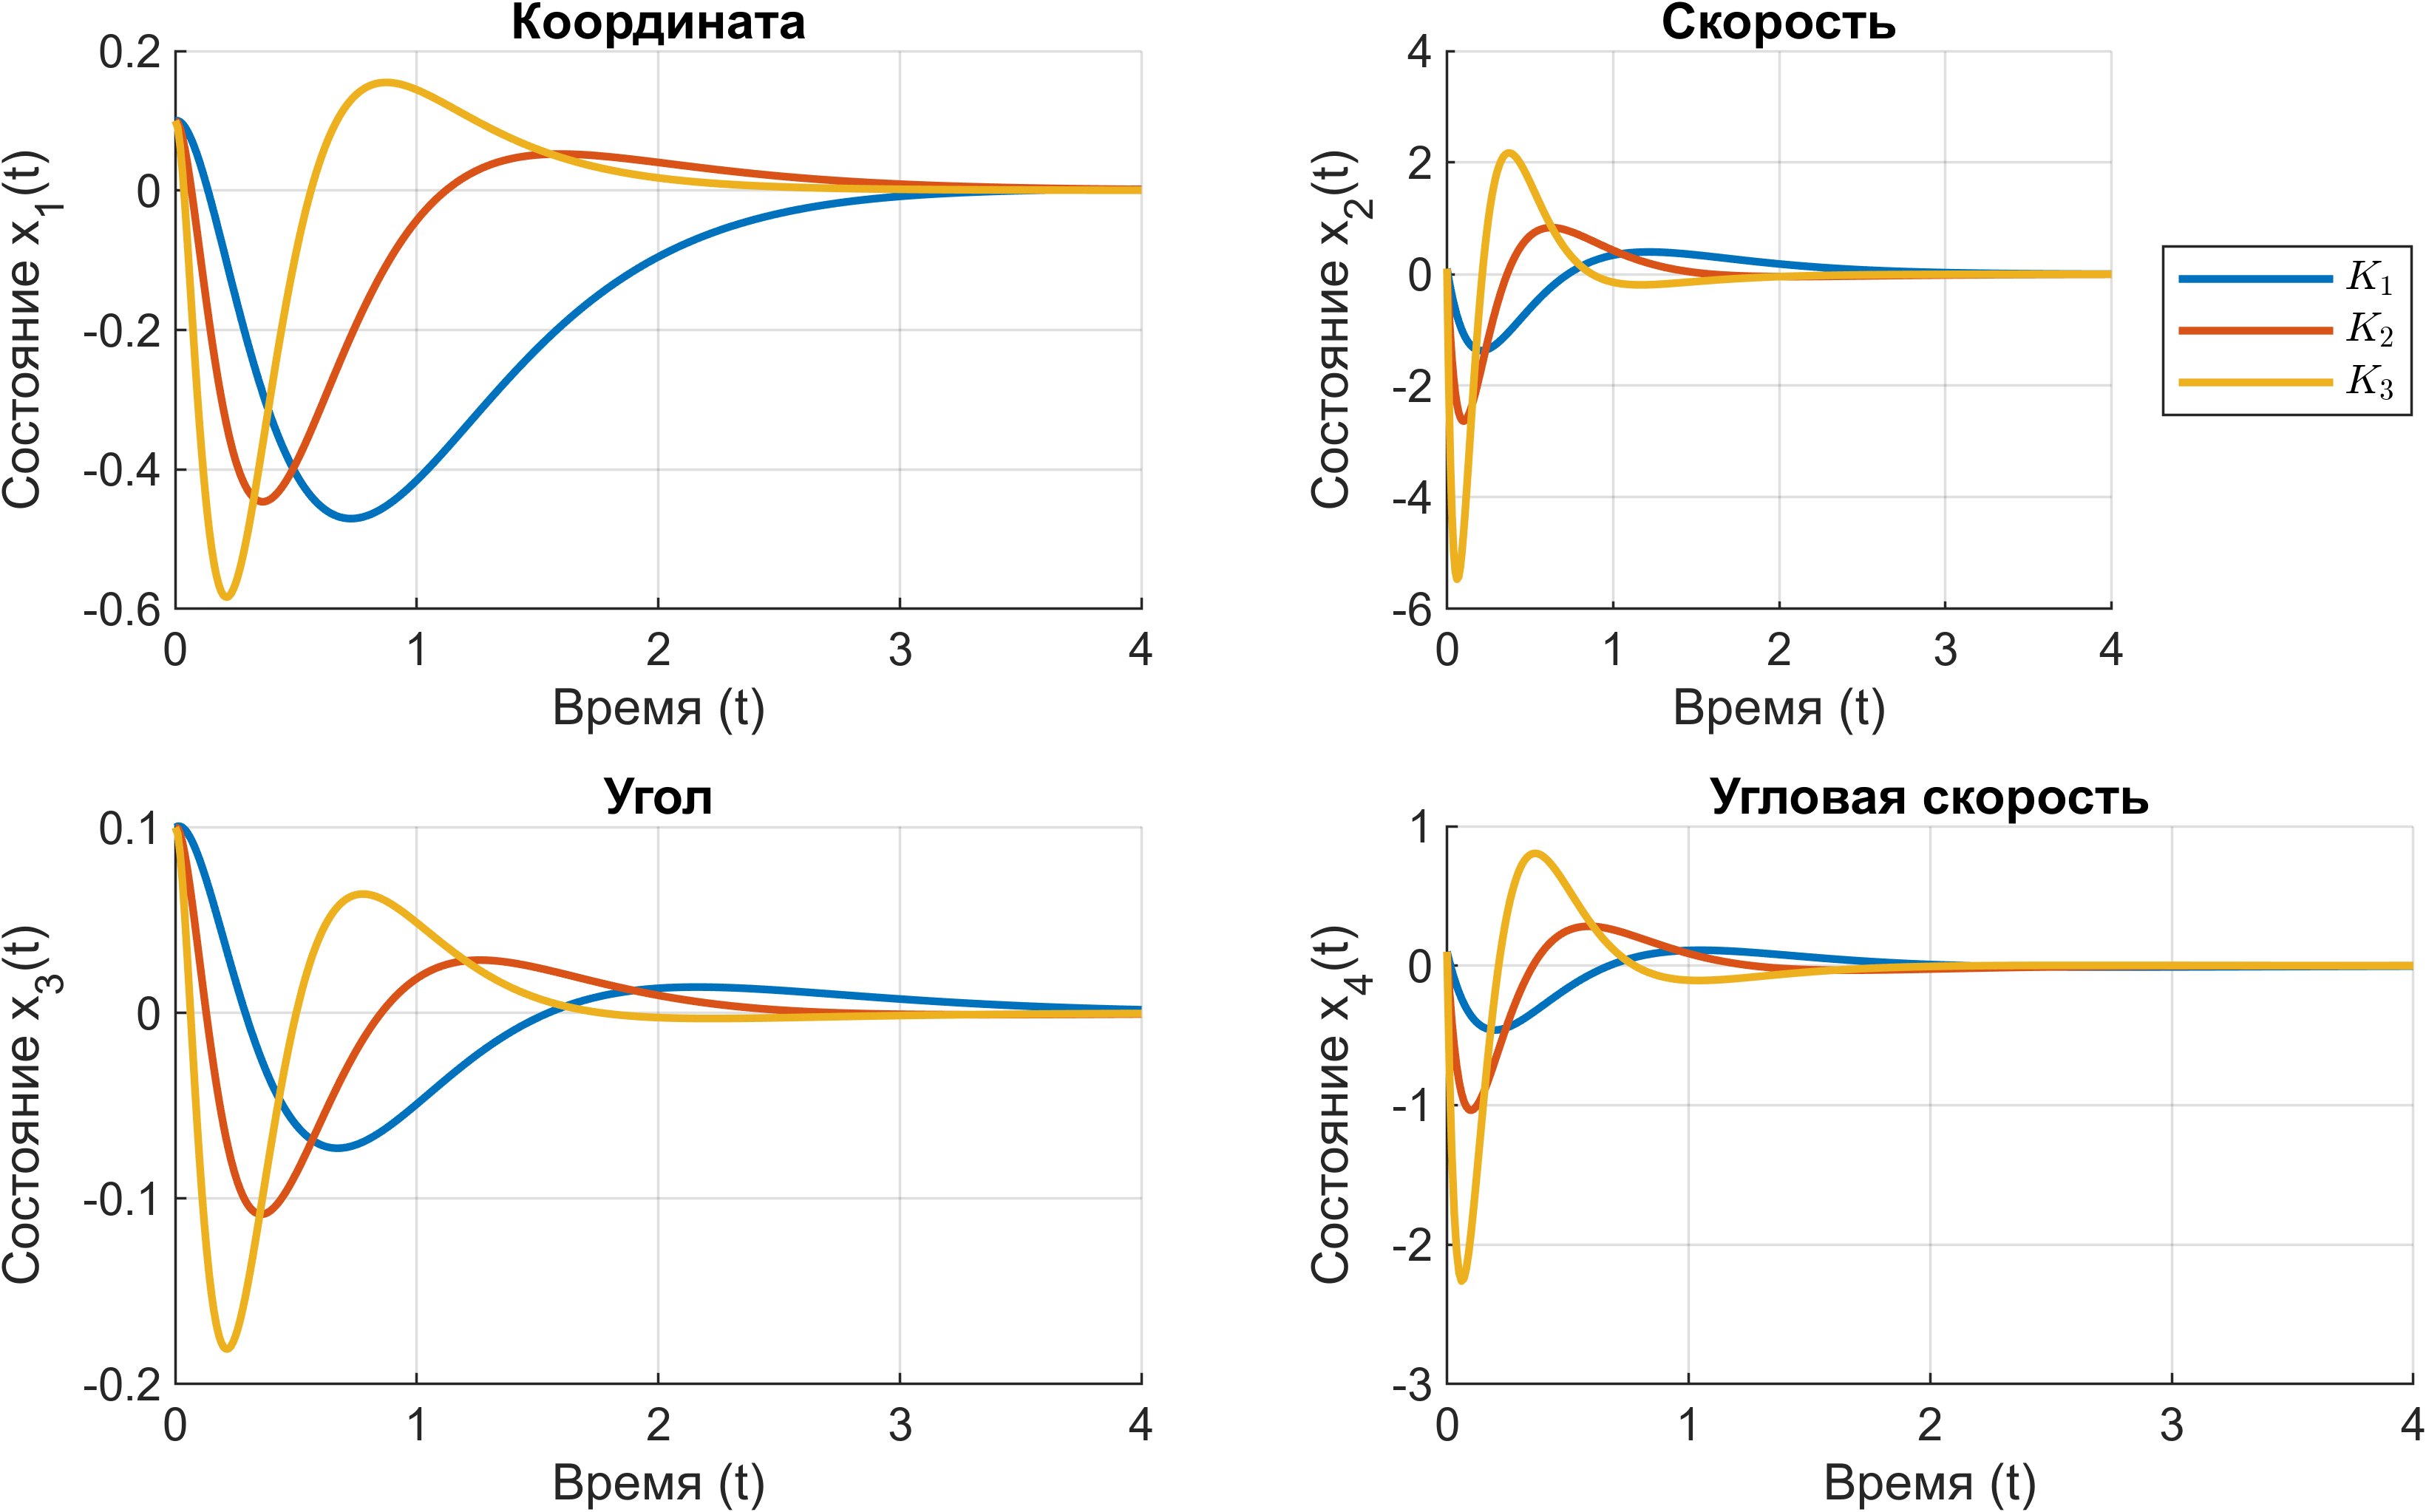
\includegraphics[width=\linewidth]{figs/3.4.watK.png}
    \caption{Моделирование работы регулятора по выходу 
    с наблюдателем пониженного порядка и разными регулятора}
    \label{fig:3.4.watK}
\end{figure}
В итоге наилучший по моему мнению регулятор - это $K_1$ и наблюдатель $Q_1$.
Их симуляцию можно увидеть на \autoref{fig:3.4.watQK}. Хотя $K_1$
наислабейший регулятор из рассматриваемых, он привел систему к устойчивому
положению за примерно 3 секунды, что достаточно быстро, если вспомнить, что
тележка имеет массу в пол тонны. В данном случае, максимально управление
составило $1654$ H, максимальное отклоние тележки - $0.5$ м, 
а максимальный угол отклонения - $5.7$ градусов (начальное положение).
\begin{figure}[H]
    \centering
    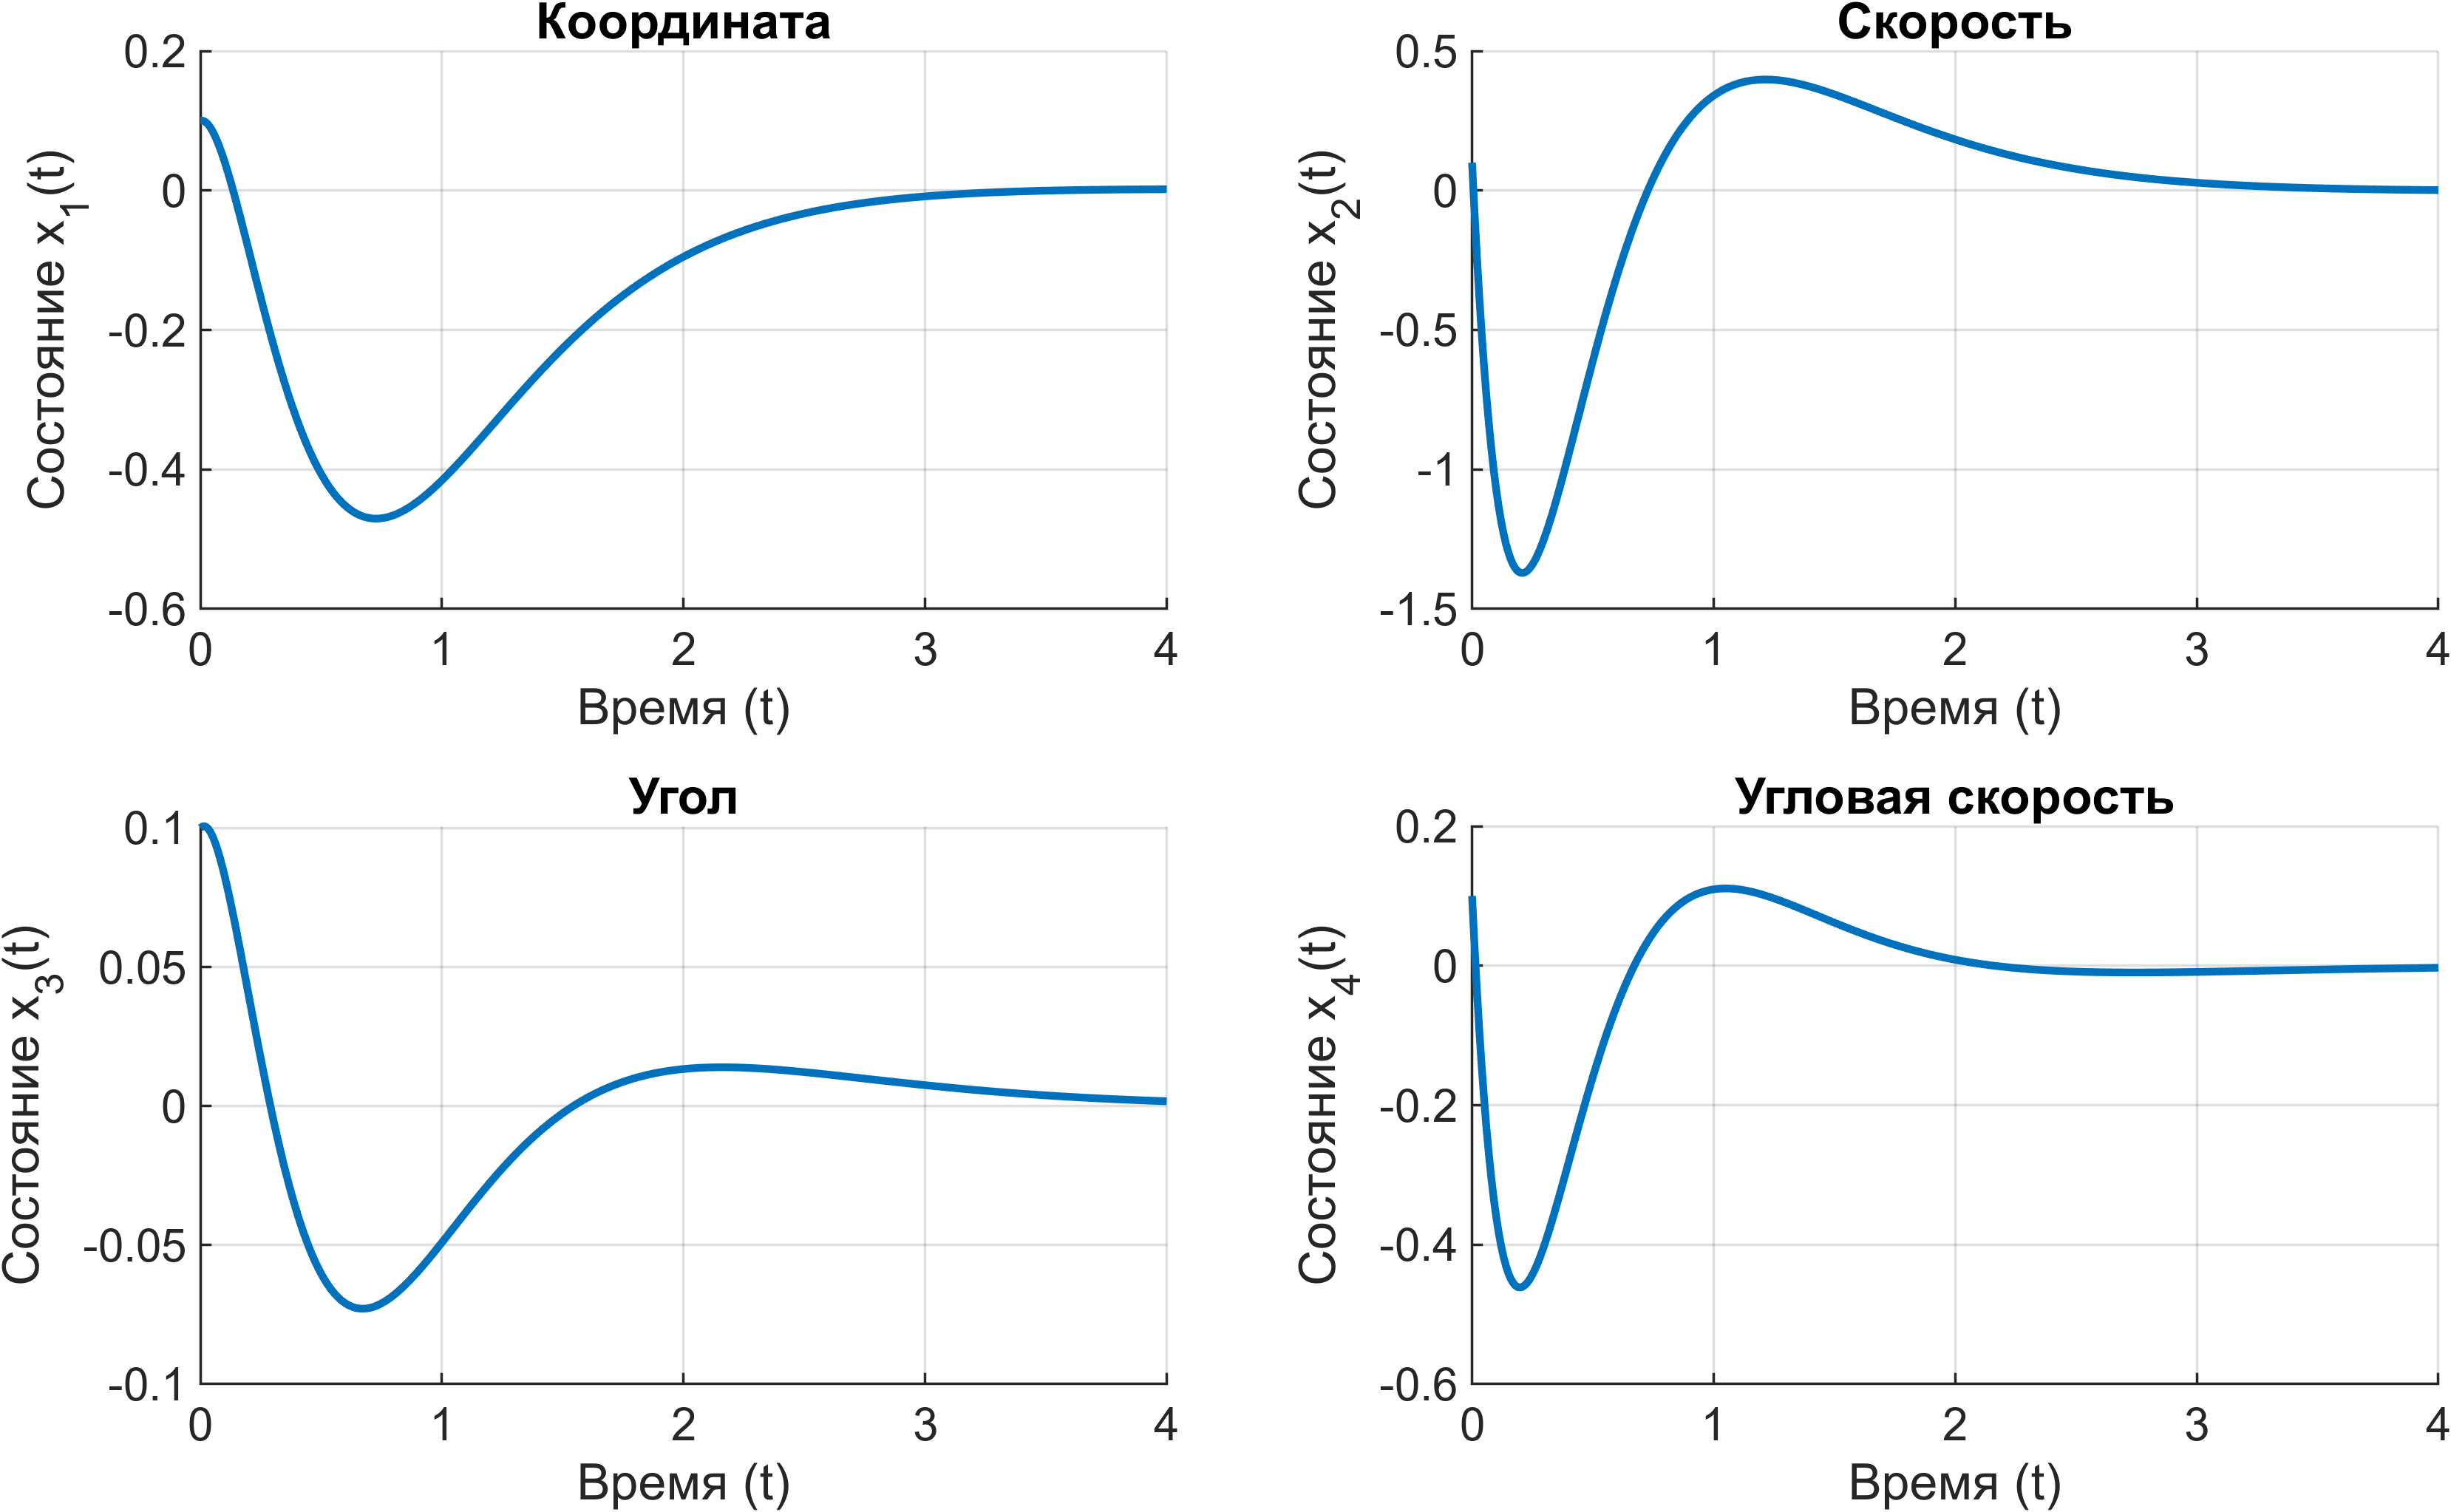
\includegraphics[width=0.8\linewidth]{figs/3.4.watQK.png}
    \caption{Моделирование работы регулятора по выходу 
    с лучшим наблюдателем  и лучшим регулятором}
    \label{fig:3.4.watQK}
\end{figure}

\chapter{Стабилизация маятника: регуляторы с заданной степенью устойчивости}

\section{Синтез регулятора по состоянию}

С помощью решения линейного матричного неравенства Ляпунова 
для экспоненциальной устойчивости:
\begin{equation*}
    PA^T+AP+2\alpha P+Y^TB^T+BY\preccurlyeq 0,\quad P\succ0,\quad K=YP^{-1},
\end{equation*}
произведем расчет регулятора \eqref{eq:3.1.reg}, основываясь на 
линейной модели \eqref{eq:sys} и степени устойчивости $\alpha=1$ замкнутой системы. 
Используя CVX, получаем:
\begin{equation*}
    K=\begin{bmatrix}
3412.0 & 5522.0 & -40870.0 & -19920.0
    \end{bmatrix},
\end{equation*}
итоговый спектр замкнутой системы $\sigma(A+BK)=\left\{\begin{array}{cccc}
-1.5\pm3.2\,\mathrm{i}&
-1.1&
-2.1
\end{array}\right\}.$
Исследуем поведение системы в зависимости от начальных условий:
\begin{equation*}
    x_{01}=\begin{bmatrix}
        7.4\\
        0.1\\
        0.1\\
        0.1
    \end{bmatrix},\quad
    x_{02}=\begin{bmatrix}
        0.1\\
         4.3\\
         0.1\\
         0.1
    \end{bmatrix},\quad
    x_{03}=\begin{bmatrix}
        0.1\\
         0.1\\
         0.5\\
         0.1
    \end{bmatrix},\quad
    x_{04}=\begin{bmatrix}
        0.1\\
        0.1\\
        0.1\\
        1.3
    \end{bmatrix},
\end{equation*}
эти начальные условия были подобраны так, что бы маятник не упал, при больших 
значениях он падал. Получается максимальное отклонение тележки $7.4$ м,
максимальная скорость тележки вдоль оси $X$ $4.3$ м/с, максимальный угол 
отклонения маятника $28.7^\circ$, максимальная угловая скорость
маятника $74.5^\circ$ в секунду.
Как можно заметить, эти начальные условия меньше стабильных начальных условий 
модального регулятора. Графики симуляции нелинейной системы 
можно увидеть на \autoref{fig:4.1.sim}. Результаты очень похожи на результаты
модального регулятора на \autoref{fig:3.1.good}.

\begin{figure}[H]
    \centering
    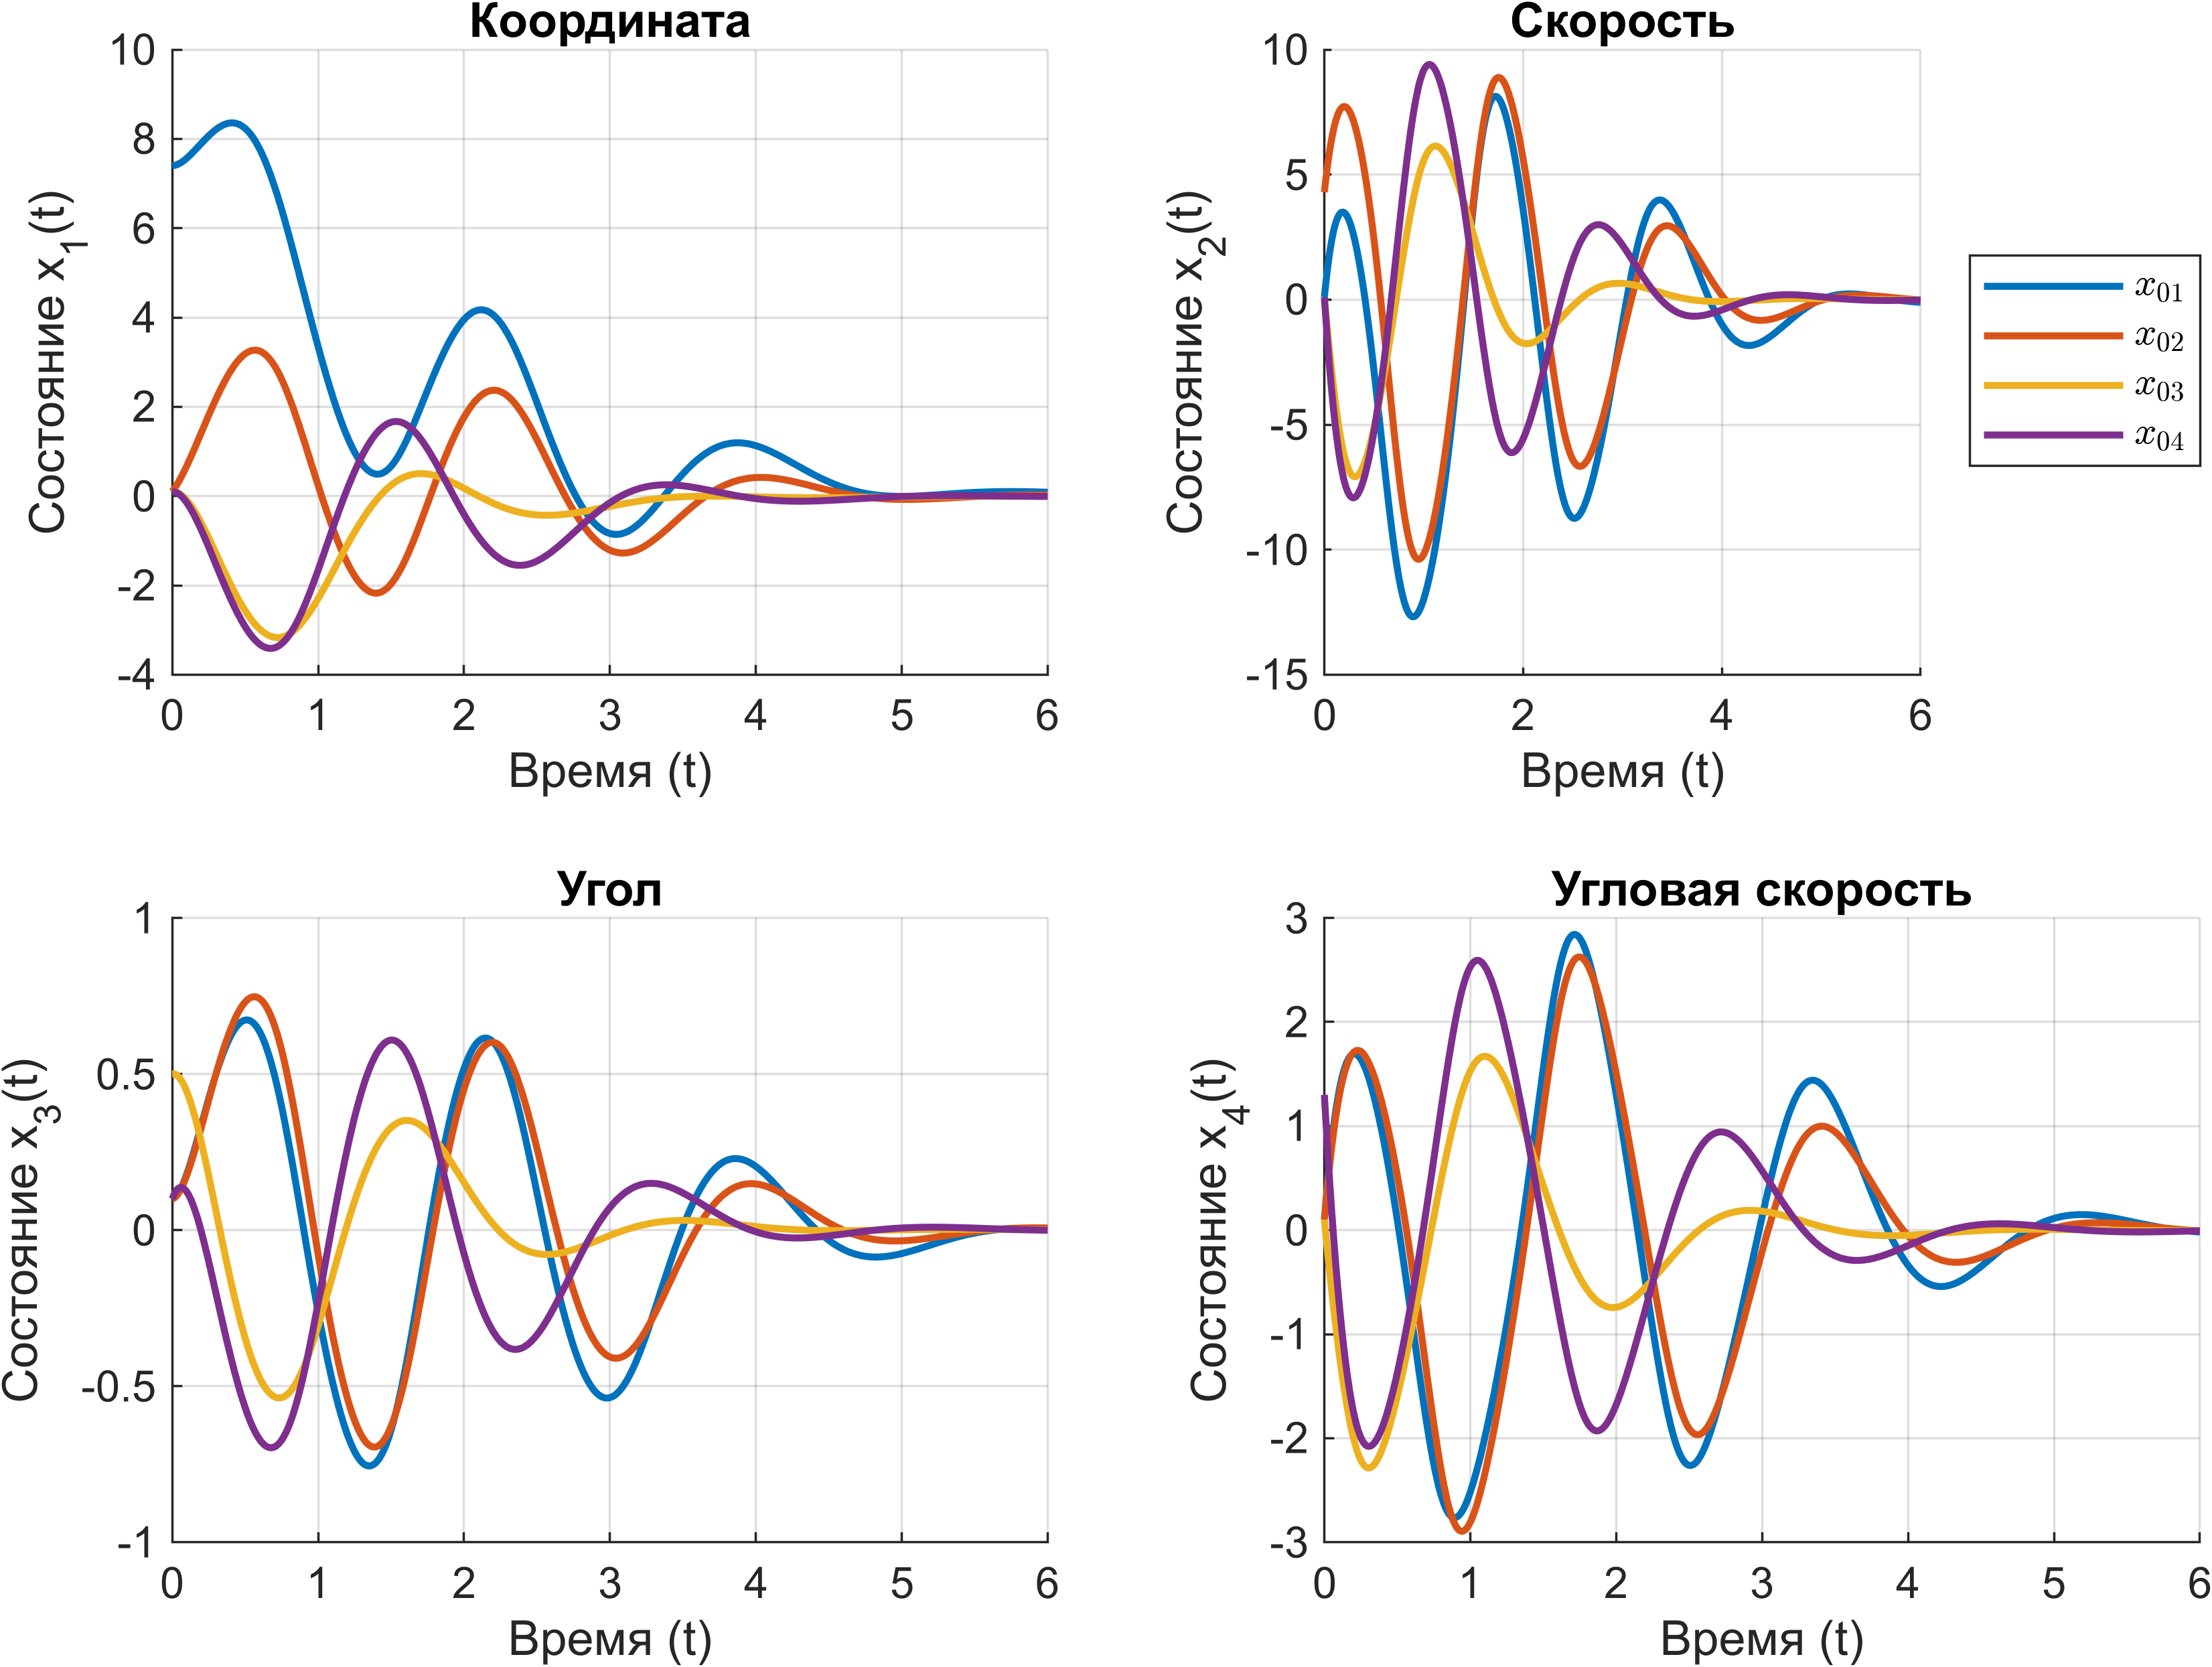
\includegraphics[width=\linewidth]{figs/4.1.sim.png}
    \caption{Моделирование работы регулятора с заданной степенью устойчивости 
    по состоянию с устойчивыми начальными условиями}
    \label{fig:4.1.sim}
\end{figure}

\section{Исследование регулятора по состоянию}

Исследуем влияние параметра $\alpha$ на максимальное отклонение маятника 
от вертикали, максимальное горизонтальное смещение тележки и максимальное 
значение управляющего сигнала при управлении нелинейной системой \eqref{eq:origsys}.
Выберем начальное состояние, где все числа $0.1$, и три степени устойчивости:
$\alpha_1=0.01$, $\alpha_2=1$, $\alpha_3=4$.
Получим следующие матрицы регуляторов:
\begin{gather*}
    K_1=\begin{bmatrix}
        26.97 & 500.6 & -12060.0 & -5862.0
    \end{bmatrix},\\
    K_2=\begin{bmatrix}
        3412.0 & 5522.0 & -40870.0 & -19920.0
    \end{bmatrix},\\
    K_3=\begin{bmatrix}
        248800.0 & 127100.0 & -822500.0 & -317300.0
    \end{bmatrix},
\end{gather*}
полчились следующие спектры замкнутых систем:
\begin{gather*}
    \sigma_1=\left\{ \begin{array}{ccc}
-2.1&
-0.059&
-0.99\pm0.96\,\mathrm{i}
    \end{array} \right\},\\
    \sigma_2=\left\{ \begin{array}{ccc}
-1.5\pm3.2\,\mathrm{i}&
-1.1&
-2.1
    \end{array} \right\},\\
    \sigma_3=\left\{ \begin{array}{cc}
-4.8\pm9.0\,\mathrm{i}&
-4.3\pm1.5\,\mathrm{i}
    \end{array} \right\}.
\end{gather*}
Результат симуляции нелинейной системы можно увидеть на \autoref{fig:4.2.sim}.
\begin{figure}[H]
    \centering
    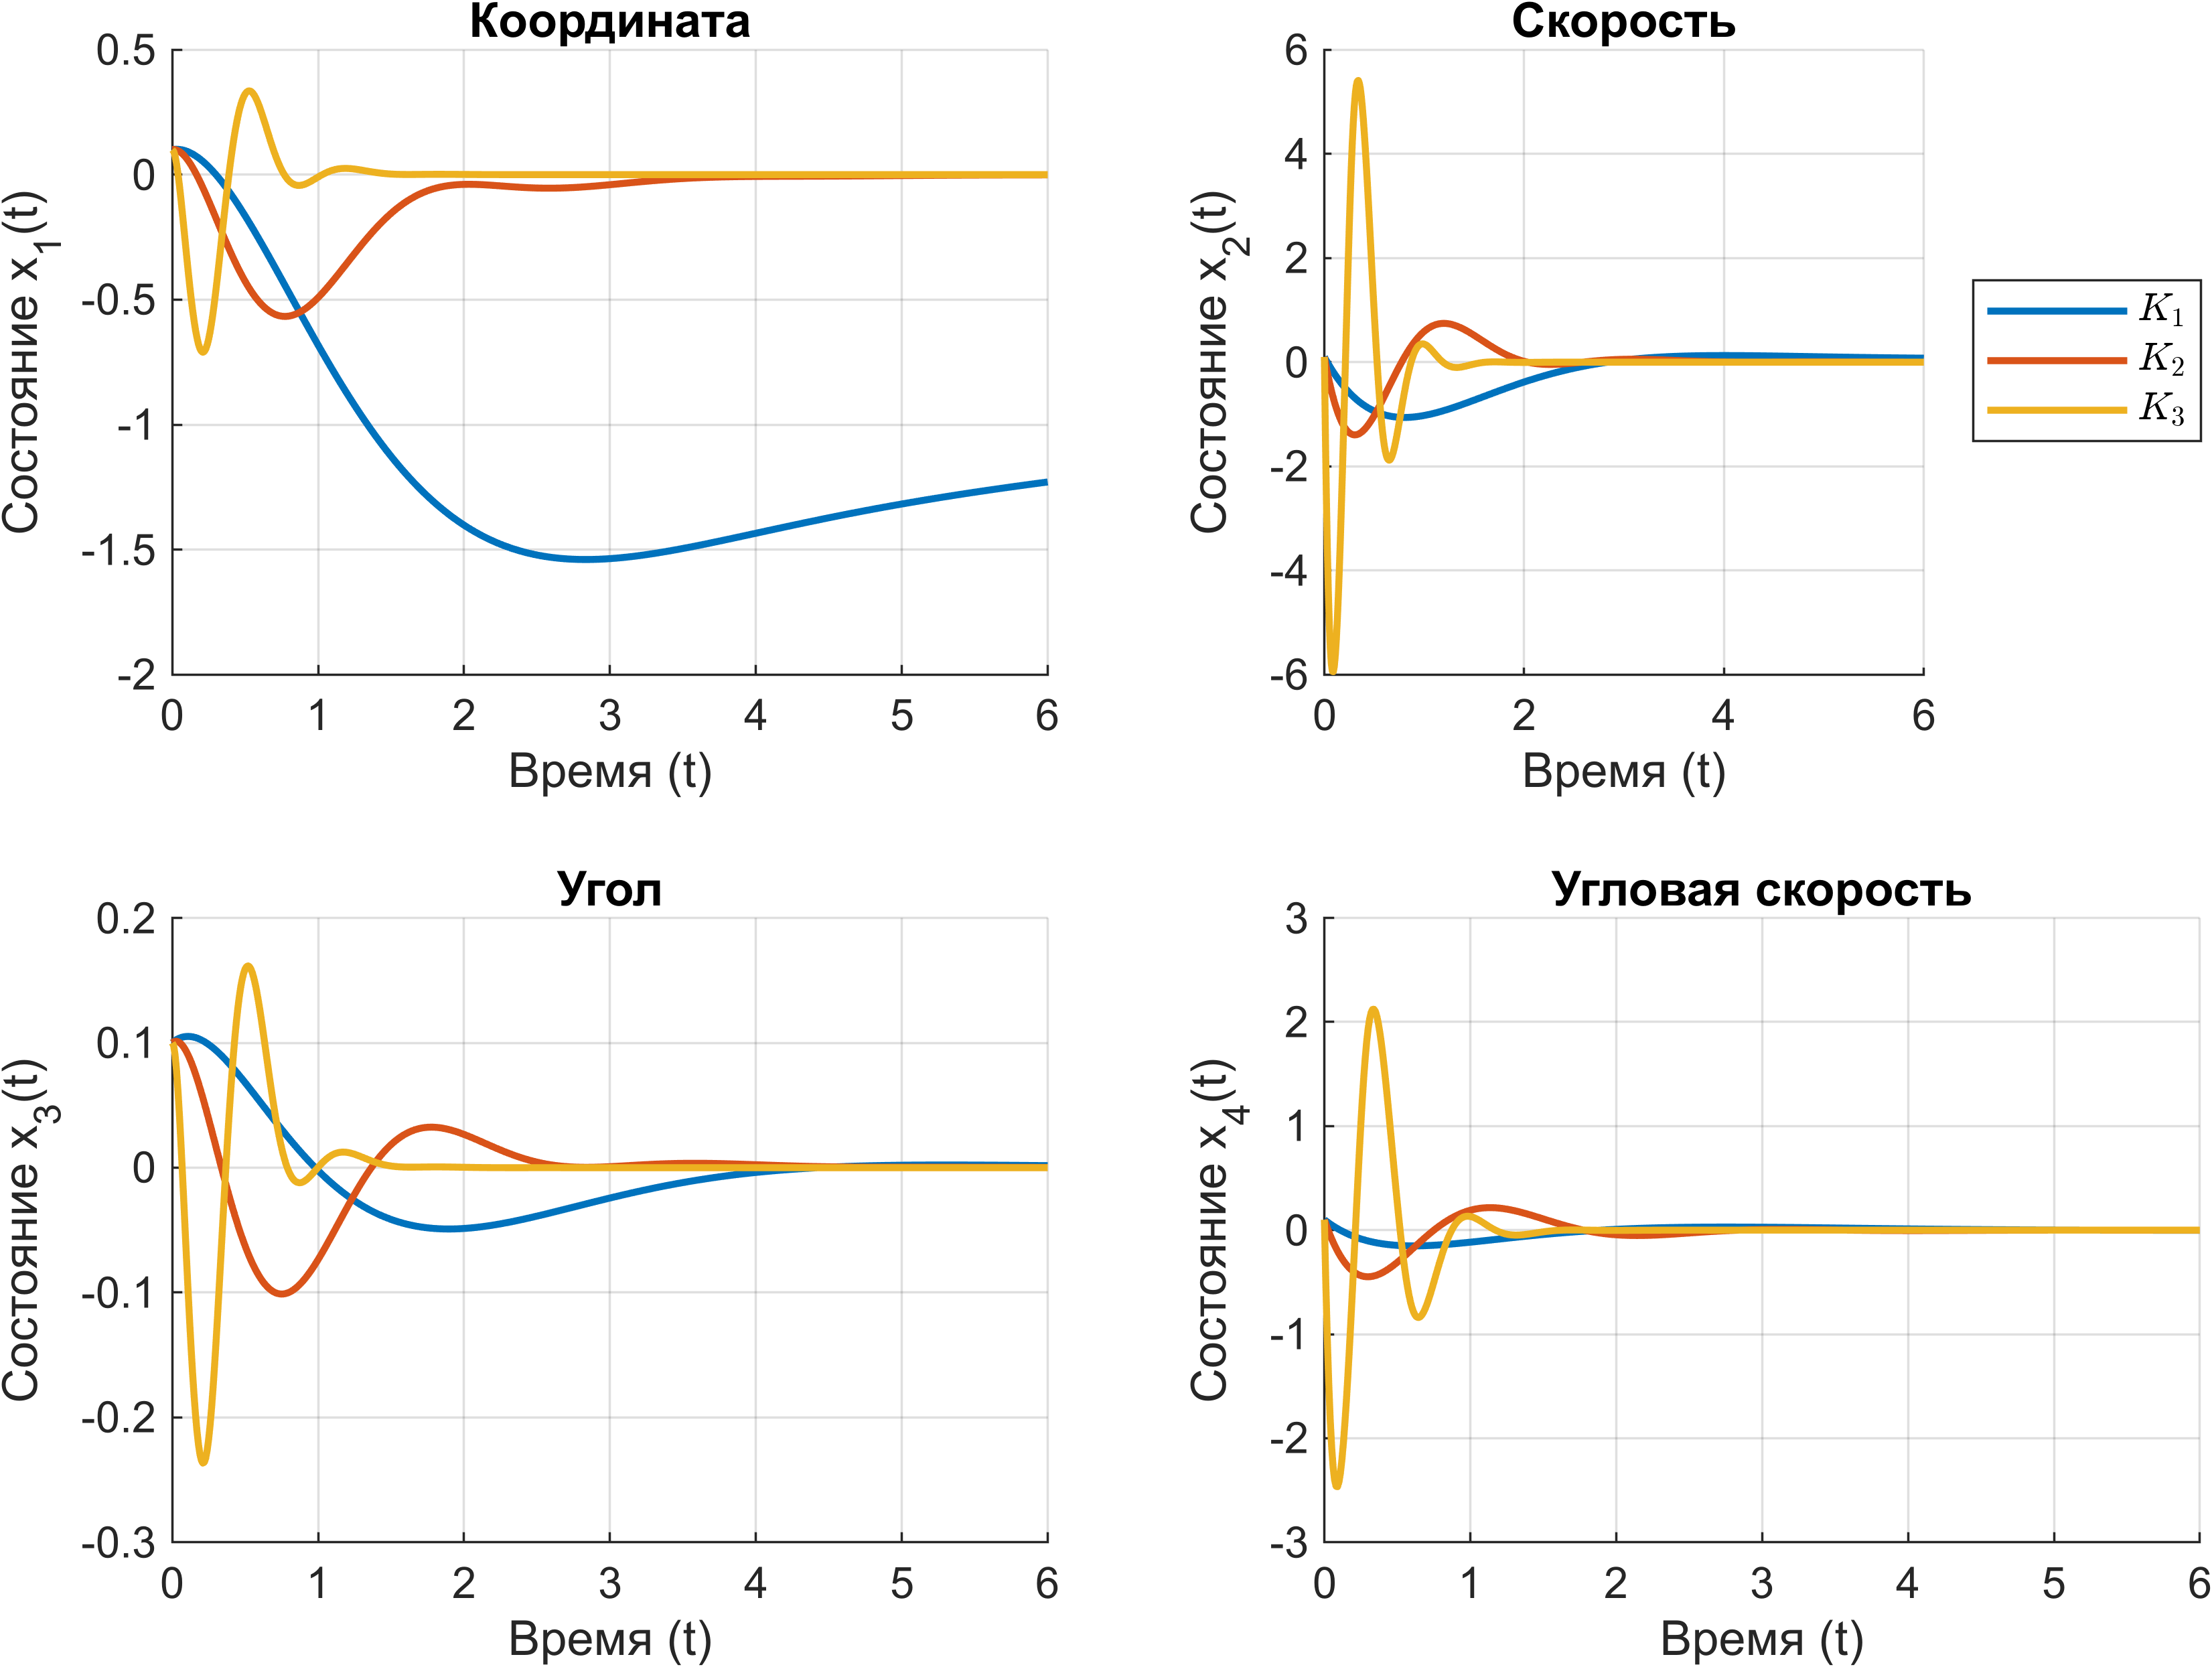
\includegraphics[width=\linewidth]{figs/4.2.sim.png}
    \caption{Моделирование работы регулятора с заданной степенью устойчивости 
    по состоянию с различными степенями устойчивости}
    \label{fig:4.2.sim}
\end{figure}
\noindent Чем больше степень устойчивости, тем быстрее сходится система.
Максимальное отклонение маятника 
от вертикали, максимальное горизонтальное смещение тележки и максимальное 
значение управляющего сигнала можно увидеть в таблице \autoref{tab:4.2.a}.
При первых двух регуляторах угол отклонения маятника не уходили дальше
начальных условий, при $K_3$ маятник отклонился в два раза больше, чем
изначальное положение. Управления, в сравнении с рассмотренными модальными 
регуляторами, требуется меньше, но и время схождения больше.

\begin{table}[H]
    \centering
    \caption{\label{tab:4.2.a}Влияние параметра $\alpha$ на характеристики системы}
    \begin{tabular}{|c|c|c|c|}
        \hline
        $\alpha$ & Макс. упр., H & Макс. откл. тележки, м & Макс. угол маятника, $^\circ$ \\
        \hline
        0.01 & 1739.8   & 1.54  & 5.7   \\
        1    & 5186.0   & 0.57  & 5.7   \\
        4    & 76388.9  & 0.71  & 13.8  \\
        \hline
    \end{tabular}
\end{table}

\section{Синтез регулятора по состоянию с ограничением на управление}
\label{sec:4.4}
Для нескольких значения параметра $\alpha_1=0.01$, $\alpha_2=1$ выполним расчет регулятора \eqref{eq:3.1.reg} 
такого, чтобы наибольшее значение модуля управляющего сигнала $u$ было 
наименьшим из возможных, сделаем это с помощью матричного неравенства
Ляпунова с дополнением:
\begin{gather*}
    P\succ0,\quad PA^T+AP+2\alpha P+Y^TB^T+BY\preccurlyeq 0,\\
    \begin{bmatrix}
        P&x_0\\x_0^T&1
    \end{bmatrix}\succ0,\quad
    \begin{bmatrix}
        P&Y^T\\Y&\mu^2I
    \end{bmatrix}\succ0.
\end{gather*}
С помощью CVX получаем матрицу регуляторов с соответствующими начальными
условиями, которые использовались при синтезе:
\begin{equation*}
    K_1=\begin{bmatrix}
0.001438 & 0.1925 & -4932.0 & -2390.0
    \end{bmatrix},\quad
        x_0=\begin{bmatrix}
        0&0.1&0&0
    \end{bmatrix},
\end{equation*}
\begin{equation}
    \label{eq:4.4.K2}
    K_2=\begin{bmatrix}
797.9 & 1665.0 & -19870.0 & -9666.0
    \end{bmatrix},\quad
    x_0=\begin{bmatrix}
        0.01&0&0&0
    \end{bmatrix},
\end{equation}
\begin{gather*}
        \sigma(A+BK_1)=\left\{\begin{array}{ccc}
        -2.1&
        -0.01\pm0.022\,\mathrm{i}&
        -0.01
    \end{array}\right\},\\
        \sigma(A+BK_2)=\left\{\begin{array}{ccc}
-1.0\pm1.5\,\mathrm{i}&
-2.1&
-1.0
\end{array}\right\}.
\end{gather*}
Исследуем работоспособность синтезированных регуляторов при управлении 
нелинейной системой \eqref{eq:origsys} в зависимости от начальных условий.

\subsection{Первая степень устойчивости}

Рассмотрим систему с регулятором $K_1$. Выберем начальные условия:
\begin{equation*}
    x_{01}=\begin{bmatrix}
        0&0.1&0&0
    \end{bmatrix}^T,\quad
    x_{02}=\begin{bmatrix}
        0.01&0.11&0.01&0.01
    \end{bmatrix}^T.
\end{equation*}
Одно из них один в один как при синтезе, а второе немного измененное, чтобы
посмотреть как система ведет себя с начальным условием, при котором синтезировался
регулятор и при небольшом отклонении от него.
Симуляцию можно увидеть на \autoref{fig:4.3.1.sim}. Как видно, 
при малейшем отклонении от начального условия система ведет себя
абсолютно по другому, имея гораздо большее время схождения по всем состояниям.
Так же если посмотреть на максимальное управление, при $x_{01}$ оно составило
$0.90$ H, а при $x_{02}$ - $73.20$ H, что, во первых очень мало по сравнению с
регуляторами без ограничения по управлению, а во вторых, при малейшем отклонении
от начального условия (при котором происходил синтез), оно увеличилось в 81 раз.
Вообще поразительно, что при массе тележки в пол тонны, и, хотя небольшом отклонении
от состояния равновесия, но получилось стабилизировать систему приложив всего лишь
$73$ H, большинство людей может сжатием кисти создать большую силу, хотя ценой
этого стало огромное максимальное отклонение тележки в $173$ м.

\begin{figure}[H]
    \centering
    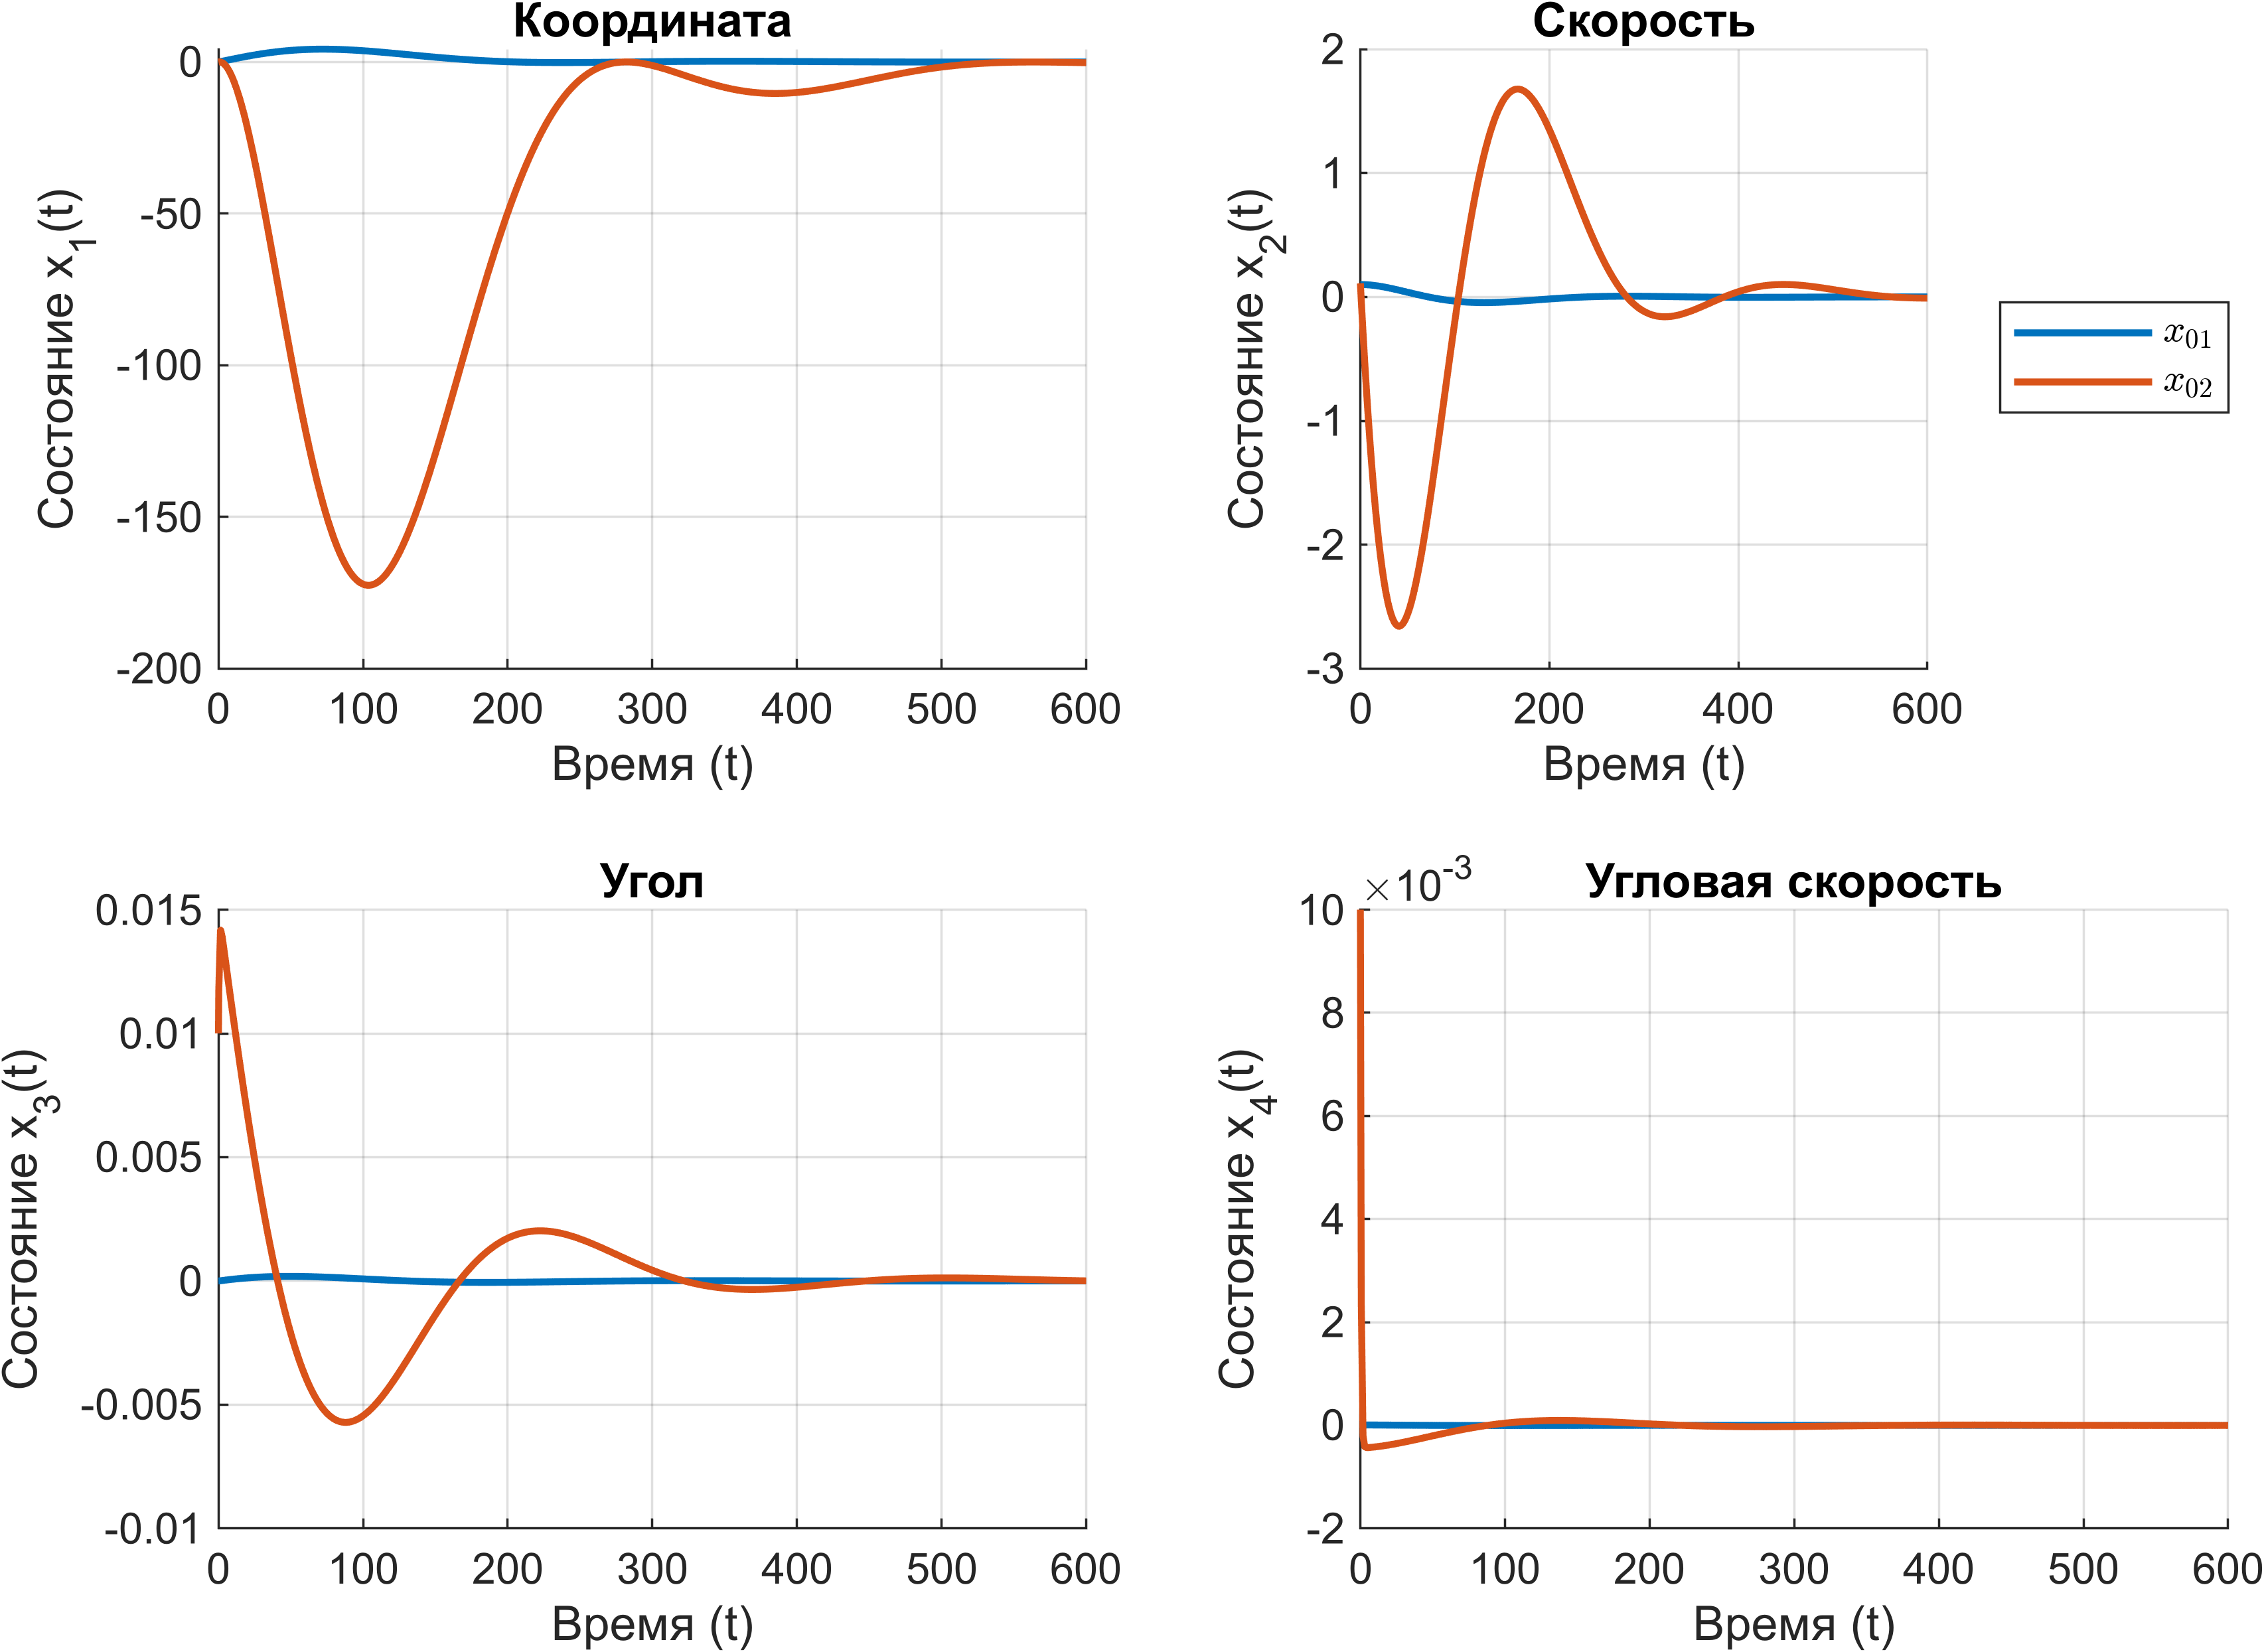
\includegraphics[width=\linewidth]{figs/4.3.1.sim.png}
    \caption{Моделирование работы регулятора с заданной степенью устойчивости
    по состоянию с ограничением на управление при $\alpha=0.01$}
    \label{fig:4.3.1.sim}
\end{figure}

\subsection{Вторая степень устойчивости}

Рассмотрим систему с регулятором $K_2$. Выберем начальные условия:
\begin{equation*}
    x_{01}=\begin{bmatrix}
        0.01&0&0&0
    \end{bmatrix}^T,\quad
    x_{02}=\begin{bmatrix}
        0.02&0.01&0.01&0.01
    \end{bmatrix}^T.
\end{equation*}
Опять же одно из них один в один как при синтезе, а второе немного измененное, чтобы
посмотреть как система ведет себя с начальным условием, при котором синтезировался
регулятор и при небольшом отклонении от него.
Симуляцию можно увидеть на \autoref{fig:4.3.2.sim}. 
"Картина" аналогична предыдущей: малейшее отклонение от "родительского" 
начального условия приводит к значительно большим отклонениям, колебаниям и
немного большему времени схождения. Сам регулятор со степепью устойчивости
$1$ более "сильный" и при $x_{01}$ требует максимальное управление в $7.98$ H, 
а при $x_{02}$ - $262.71$ H. Разница в управлении не такая большая, как в
первом случае, но все равно в $32$ раза больше, чем при синтезе.

\begin{figure}[H]
    \centering
    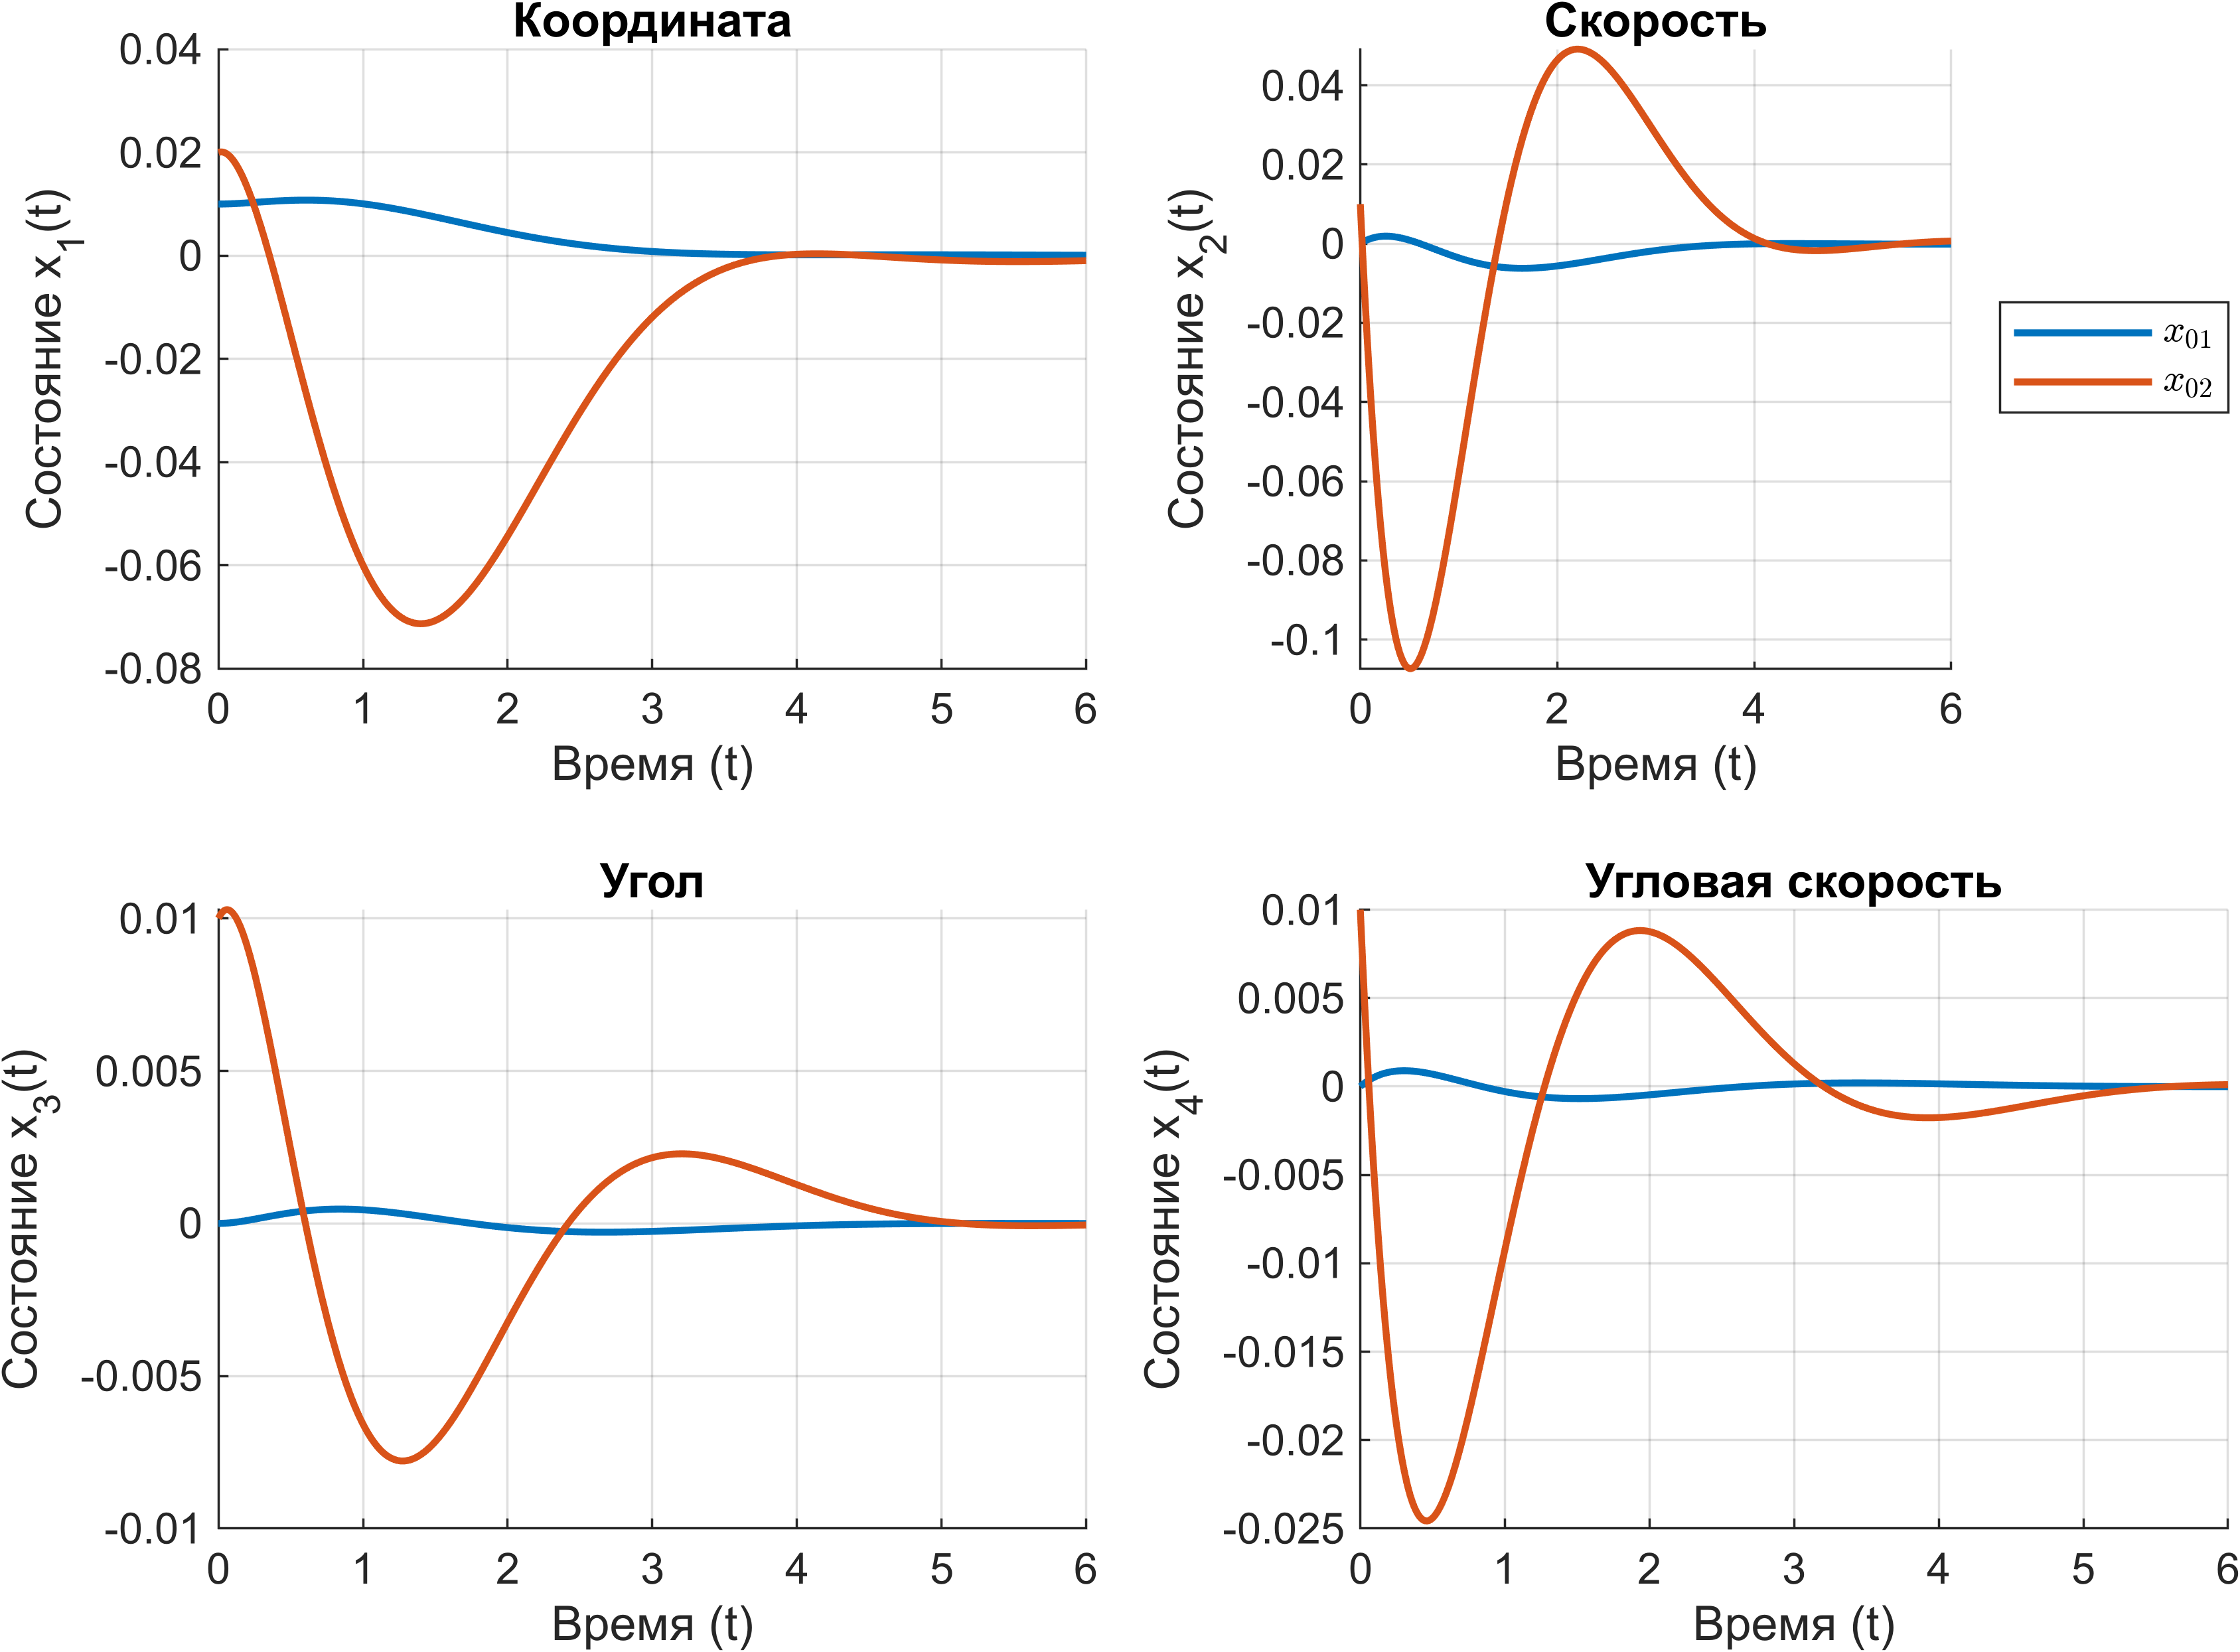
\includegraphics[width=\linewidth]{figs/4.3.2.sim.png}
    \caption{Моделирование работы регулятора с заданной степенью устойчивости
    по состоянию с ограничением на управление при $\alpha=1$}
    \label{fig:4.3.2.sim}
\end{figure}

\section{Синтез наблюдателя}

С помощью решения линейного матричного неравенства Ляпунова для 
экспоненциальной устойчивости:
\begin{equation*}
    A^TQ+QA+2\alpha Q+C^TY^T+YC\preccurlyeq0,\quad Q\succ0,\quad
    L=Q^{-1}Y,
\end{equation*}
произведем расчет наблюдателя полной размерности \eqref{eq:3.3.estfull}, 
основываясь на линейной модели \eqref{eq:sys} с тремя степенями устойчивости:
\begin{equation*}
    \alpha_1=0.01,\quad \alpha_2=1,\quad \alpha_3=4.
\end{equation*}
Получим следующие матрицы наблюдателя:
\begin{equation*}
    L_1=\begin{bmatrix}
-0.9056 & -0.04686\\
-1.309 & -0.1381\\
0.04686 & -0.9056\\
0.01601 & -5.566
    \end{bmatrix},\quad
    L_2=\begin{bmatrix}
-4.978 & -0.1295\\
-9.263 & -0.3371\\
0.1295 & -4.978\\
0.215 & -13.52
    \end{bmatrix},\quad
    L_3=\begin{bmatrix}
-4.978 & -0.1295\\
-9.263 & -0.3371\\
0.1295 & -4.978\\
0.215 & -13.52
    \end{bmatrix},
\end{equation*}
со следующими спектрами ошибок наблюдателя:
\begin{gather*}
    \sigma_1=\left\{ \begin{array}{cc}
-0.46\pm1.1\,\mathrm{i}&
-0.45\pm1.0\,\mathrm{i}
    \end{array} \right\},\\
    \sigma_2=\left\{ \begin{array}{cc}
-2.5\pm1.8\,\mathrm{i}&
-2.5\pm1.7\,\mathrm{i}
    \end{array} \right\},\\
    \sigma_3=\left\{ \begin{array}{cc}
-9.6\pm5.6\,\mathrm{i}&
-9.5\pm5.5\,\mathrm{i}
    \end{array} \right\}.
\end{gather*}
\begin{figure}[H]
    \centering
    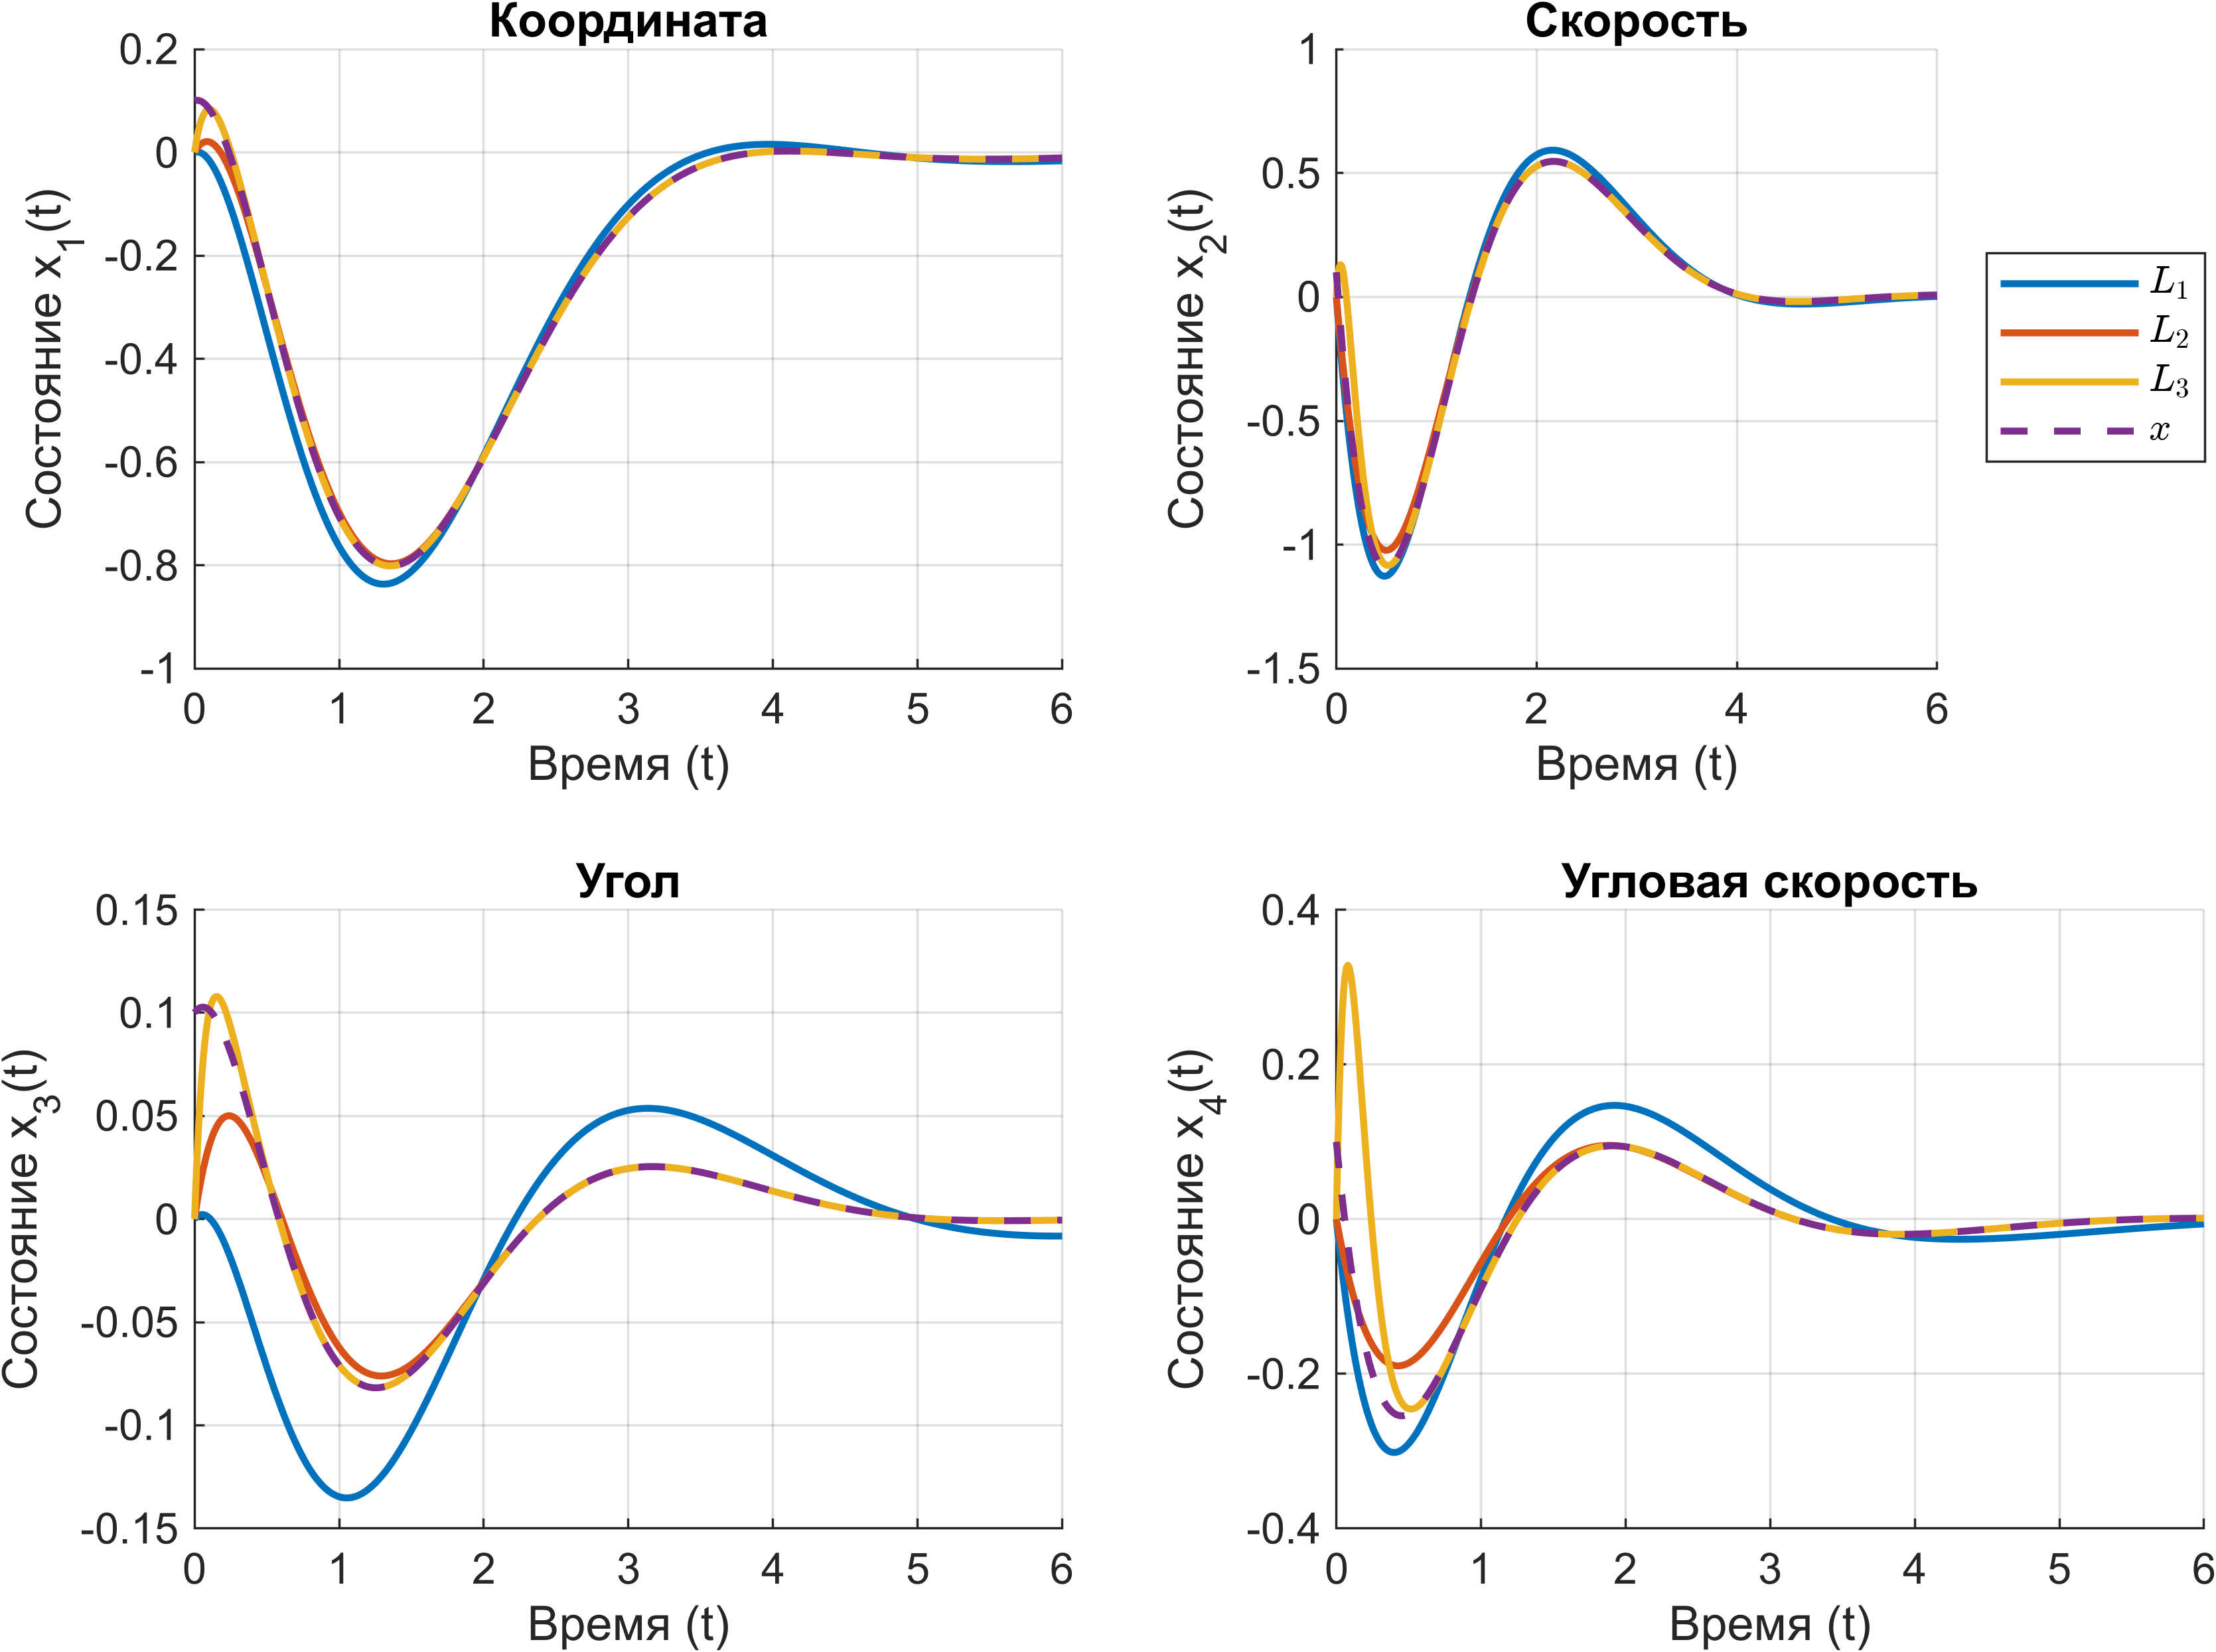
\includegraphics[width=0.8\linewidth]{figs/4.5.sim.png}
    \caption{Моделирование работы регулятора с заданной степенью устойчивости
    по состоянию с наблюдателем полного порядка}
    \label{fig:4.5.sim}
\end{figure}
\begin{figure}[H]
    \centering
    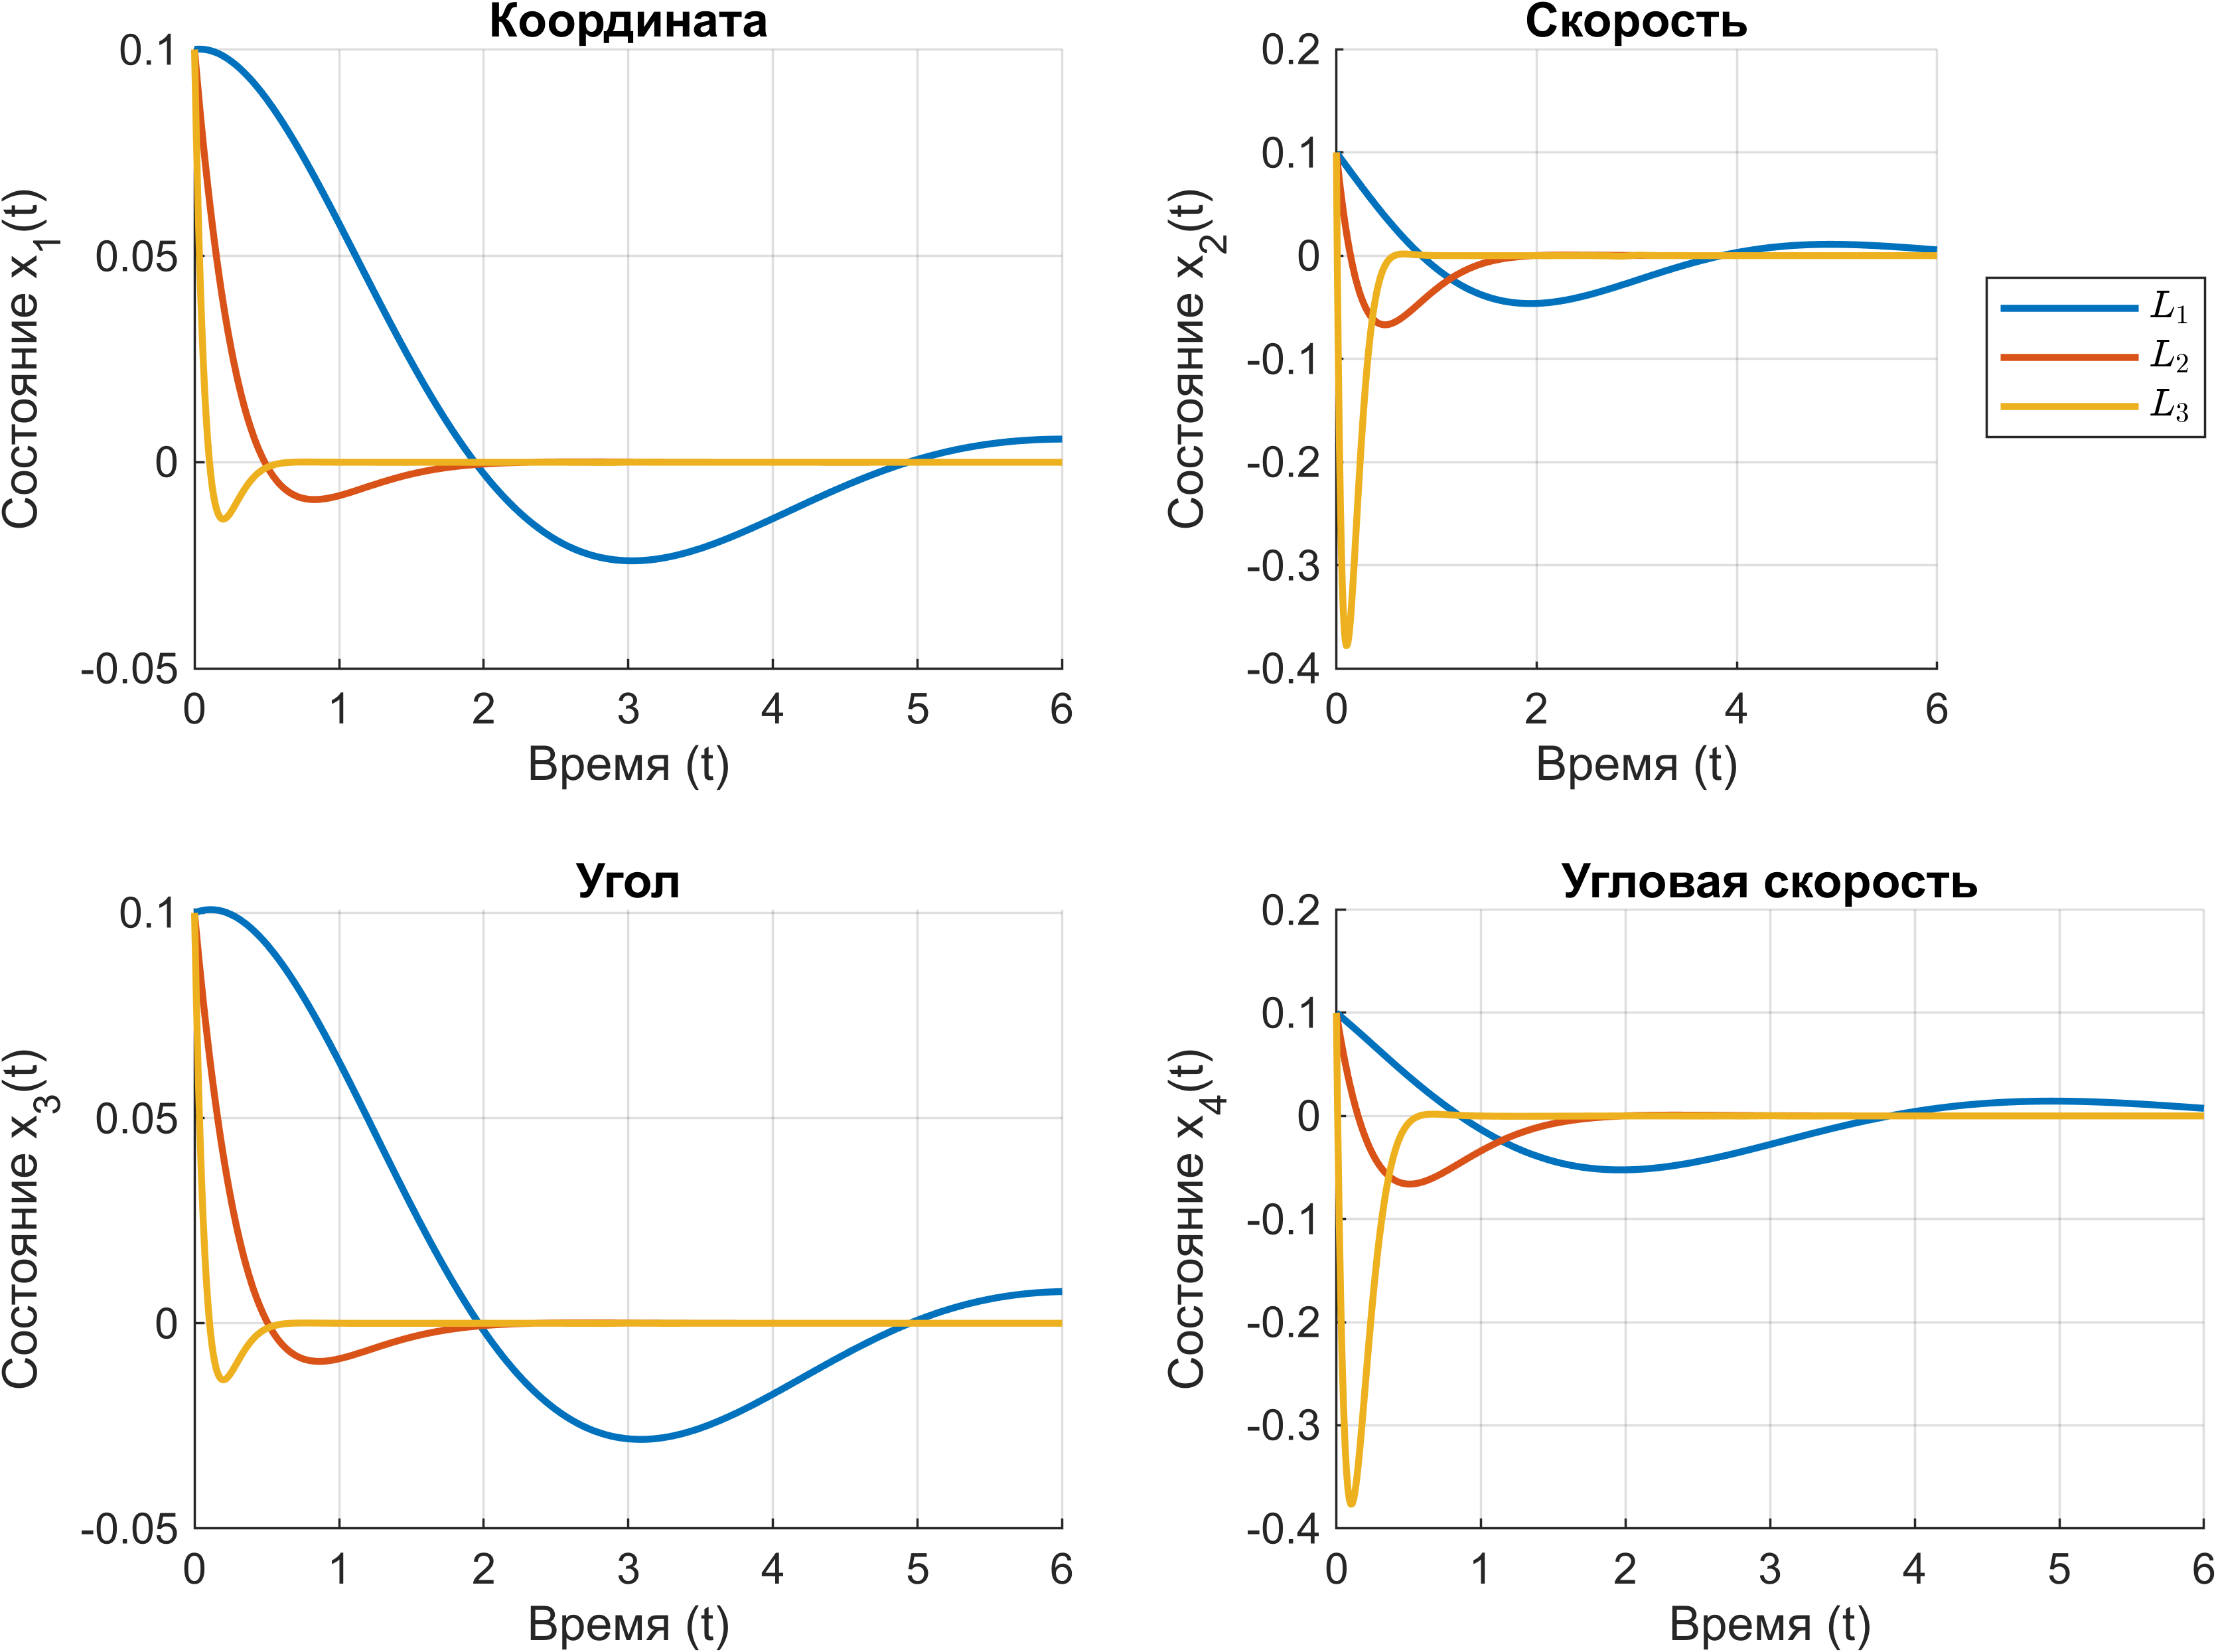
\includegraphics[width=0.8\linewidth]{figs/4.5.sim.err.png}
    \caption{Ошибка наблюдателя полного порядка}
    \label{fig:4.5.sim.err}
\end{figure}
\indent Используем регулятор $K_2$ из \autoref{sec:4.4}, который лучше всего
показал по моему мнению.
Результат симуляции нелинейной системы можно увидеть на \autoref{fig:4.5.sim},
а ошибка наблюдателя полного порядка представлена на \autoref{fig:4.5.sim.err}.
Система начинала из состояния, где все числа $0.1$, а
наблюдатель из нулевого состояния. Как видно, наблюдатель отлично работает;
чем больше степень устойчивости, тем быстрее система сходится.

\section{Синтез регулятора по выходу}
На основе линейных матричных неравенств построим регулятор, стабилизирующий 
маятник и тележку в условиях, когда измерению доступны только сигналы 
$y_1$ и $y_2$. Воспользуемся наблюдателями и регулятором из предыдущего
пункта, но будем использовать вид регулятора как в \eqref{eq:3.3.estred}.
Результат симуляции нелинейной системы можно увидеть на \autoref{fig:4.6.sim},
а ошибка наблюдателя представлена на \autoref{fig:4.6.sim.err}.
Система успешно стабилизировалась, в сравнении с управлением по состоянию,
отчетлива видна задержка.
\begin{figure}[H]
    \centering
    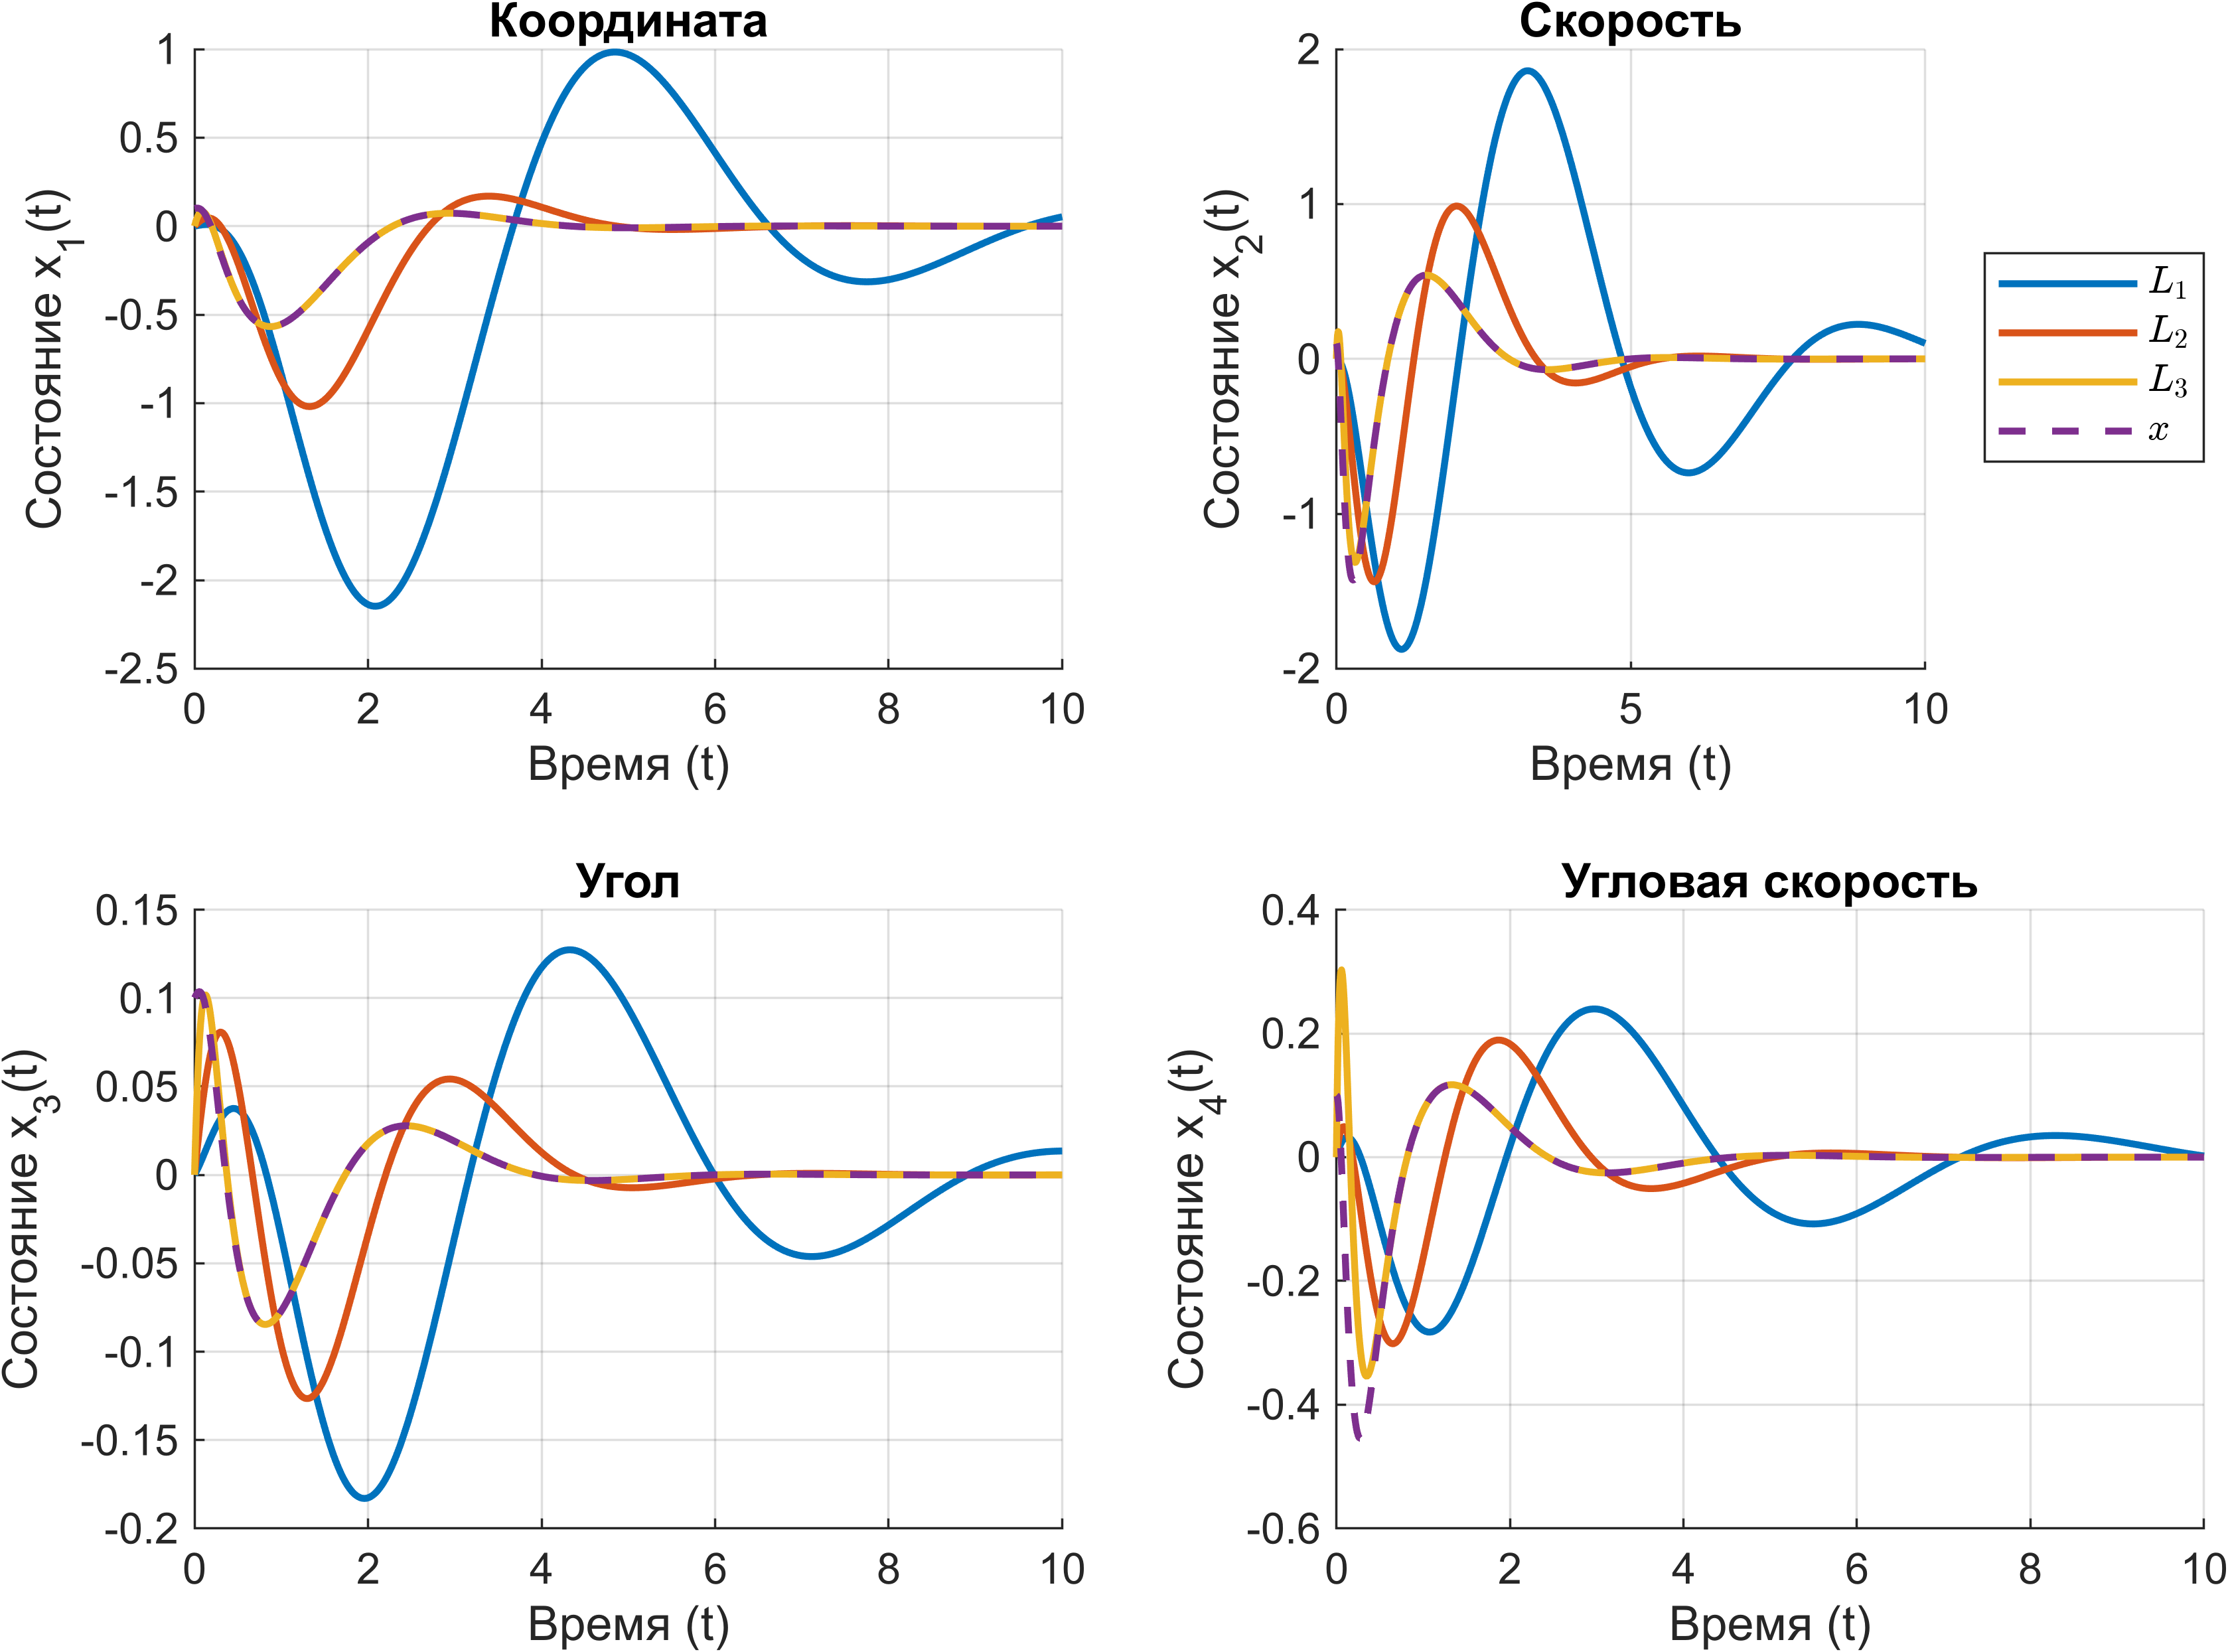
\includegraphics[width=\linewidth]{figs/4.6.sim.png}
    \caption{Моделирование работы регулятора с заданной степенью устойчивости
    по выходу с наблюдателем полного порядка}
    \label{fig:4.6.sim}
\end{figure}
\begin{figure}[H]
    \centering
    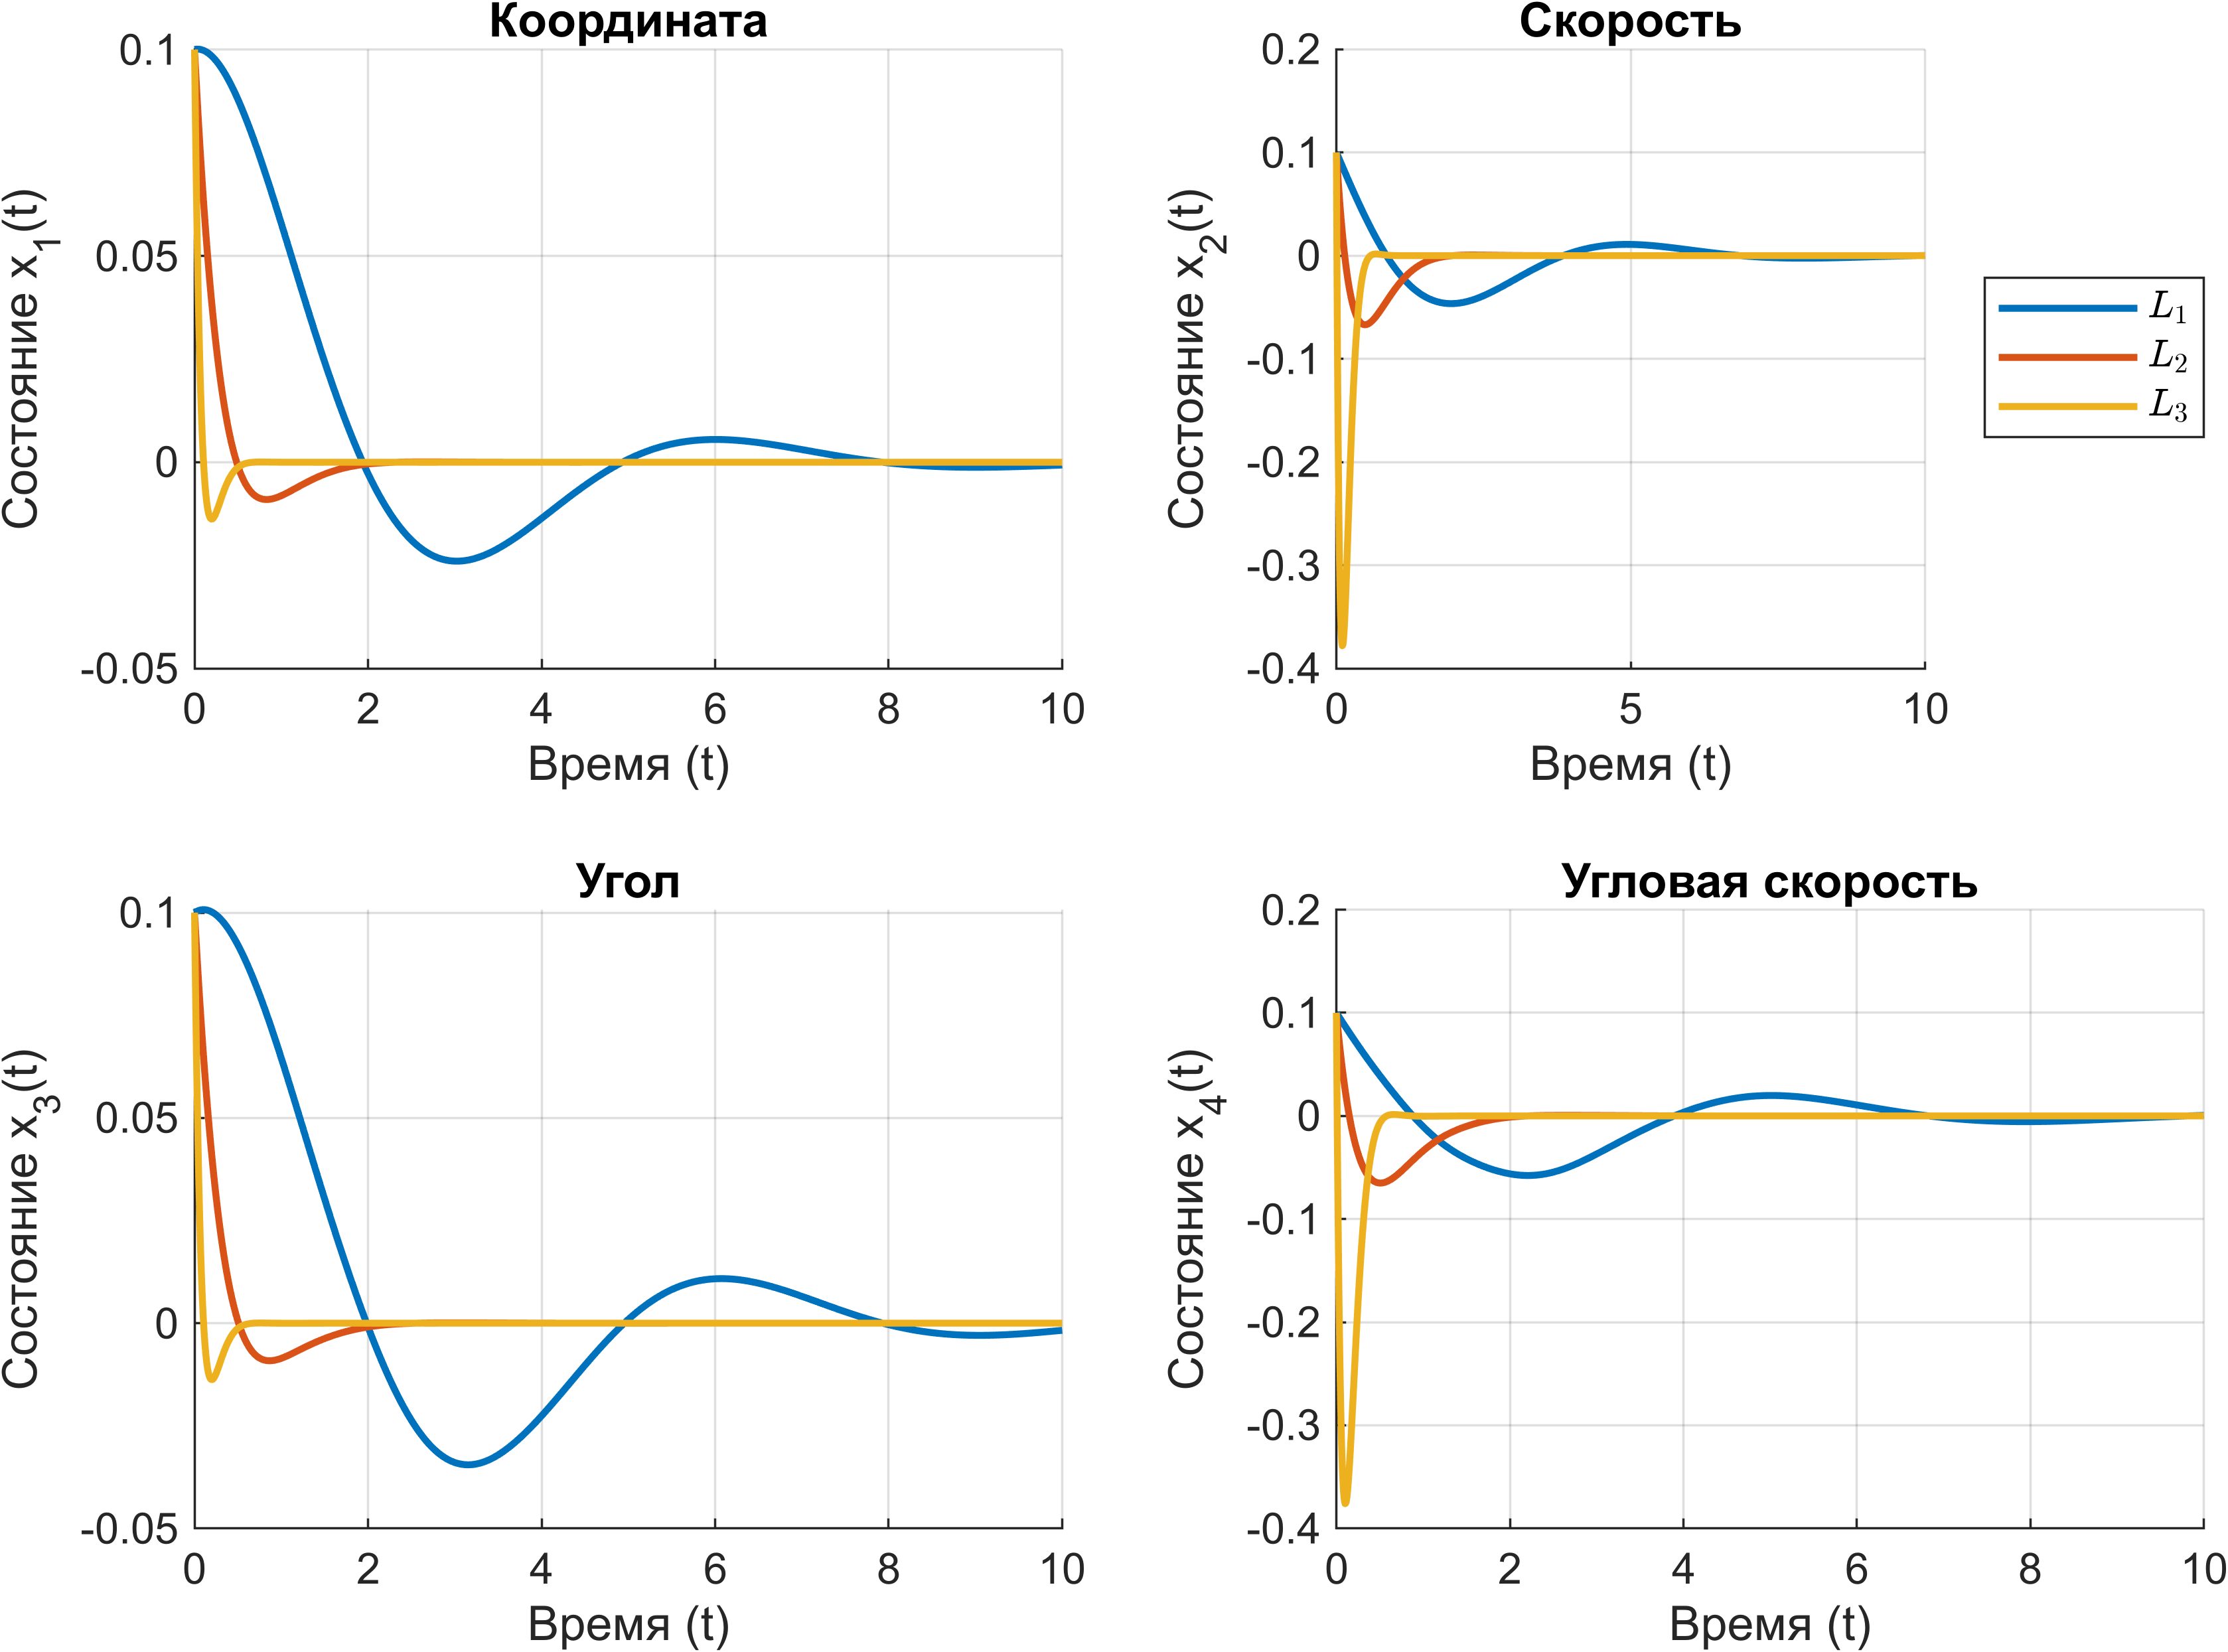
\includegraphics[width=\linewidth]{figs/4.6.sim.err.png}
    \caption{Ошибка наблюдателя полного порядка}
    \label{fig:4.6.sim.err}
\end{figure}

\chapter{Слежение и компенсация}

\section{Решение задачи компенсации}

Зададим сигнал $f$ в модели \eqref{eq:sys} как сумму пяти гармоник:
\begin{equation*}
    f(t)=\sin(t)+0.9\cos(2t)+0.8\sin(4t)+0.7\cos(8t)+0.6\sin(16t),
\end{equation*} 
тогда получаем следующий генератор:
\begin{equation}
    \label{eq:5.1.gen}
    \begin{cases}
        \dot w_f=\Gamma_f w_f\\
        f = Y_fw_f
    \end{cases},\quad w_f(0),
\end{equation}
где
\begin{equation*}
    \Gamma_f=\begin{bmatrix}
0 & -1 & 0 & 0 & 0 & 0 & 0 & 0 & 0 & 0\\
1 & 0 & 0 & 0 & 0 & 0 & 0 & 0 & 0 & 0\\
0 & 0 & 0 & -2 & 0 & 0 & 0 & 0 & 0 & 0\\
0 & 0 & 2 & 0 & 0 & 0 & 0 & 0 & 0 & 0\\
0 & 0 & 0 & 0 & 0 & -4 & 0 & 0 & 0 & 0\\
0 & 0 & 0 & 0 & 4 & 0 & 0 & 0 & 0 & 0\\
0 & 0 & 0 & 0 & 0 & 0 & 0 & -8 & 0 & 0\\
0 & 0 & 0 & 0 & 0 & 0 & 8 & 0 & 0 & 0\\
0 & 0 & 0 & 0 & 0 & 0 & 0 & 0 & 0 & -16\\
0 & 0 & 0 & 0 & 0 & 0 & 0 & 0 & 16 & 0
     \end{bmatrix},\quad
        Y_f=\begin{bmatrix}
    1 \\ 0 \\ 1 \\ 0 \\ 1 \\ 0 \\ 1 \\ 0 \\ 1 \\ 0
        \end{bmatrix}^T,\quad
        w_f(0)=\begin{bmatrix}
0\\
-1\\
0.9\\
0\\
0\\
-0.8\\
0.7\\
0\\
0\\
-0.6
        \end{bmatrix}.
\end{equation*}
Построим компенсирующий регулятор, гарантирующий выполнение условия
\begin{equation}
    \label{eq:5.1.aim}
    \lim_{t \to \infty} \| \varphi(t) \| = 0.
\end{equation}
Для этого составим регулируемый выход:
\begin{equation*}
    z=C_Zx,\quad C_Z=\begin{bmatrix}
        0 & 0 & 1 & 0
    \end{bmatrix}.
\end{equation*}
Компенсирующий регулятор имеет следующий вид:
\begin{equation}
    \label{eq:5.1.reg}
    u=K_1x+K_2w_f.
\end{equation}
В качестве "feedback" компоненты используем \eqref{eq:4.4.K2}:
\begin{equation*}
    K_1=\begin{bmatrix}
        797.9 & 1665.0 & -19870.0 & -9666.0
    \end{bmatrix}.
\end{equation*}
Для нахождения "feedforward" компоненты с помощью CVX решим следующую систему
\begin{equation*}
    \begin{cases}
        P\Gamma_f-AP=BY+D\\
        C_ZP=0
    \end{cases}
\end{equation*}
и получим
\begin{equation*}
    K_2=Y-K_1P=\begin{bmatrix}
-91.01 & 117.2 & -48.9 & 58.59 & -38.37 & 29.29 & -35.74 & 14.65 & -35.08 & 7.323
    \end{bmatrix}
\end{equation*}
Моделирование линейной модели \eqref{eq:sys} можно увидеть на 
\autoref{fig:5.1.lin}. Нелинейной модели \eqref{eq:origsys} на
\autoref{fig:5.1.nonlin}. Графики идентичны, и в обоих случаях
выполняется целевое условие \eqref{eq:5.1.aim}.

\begin{figure}[H]
    \centering
    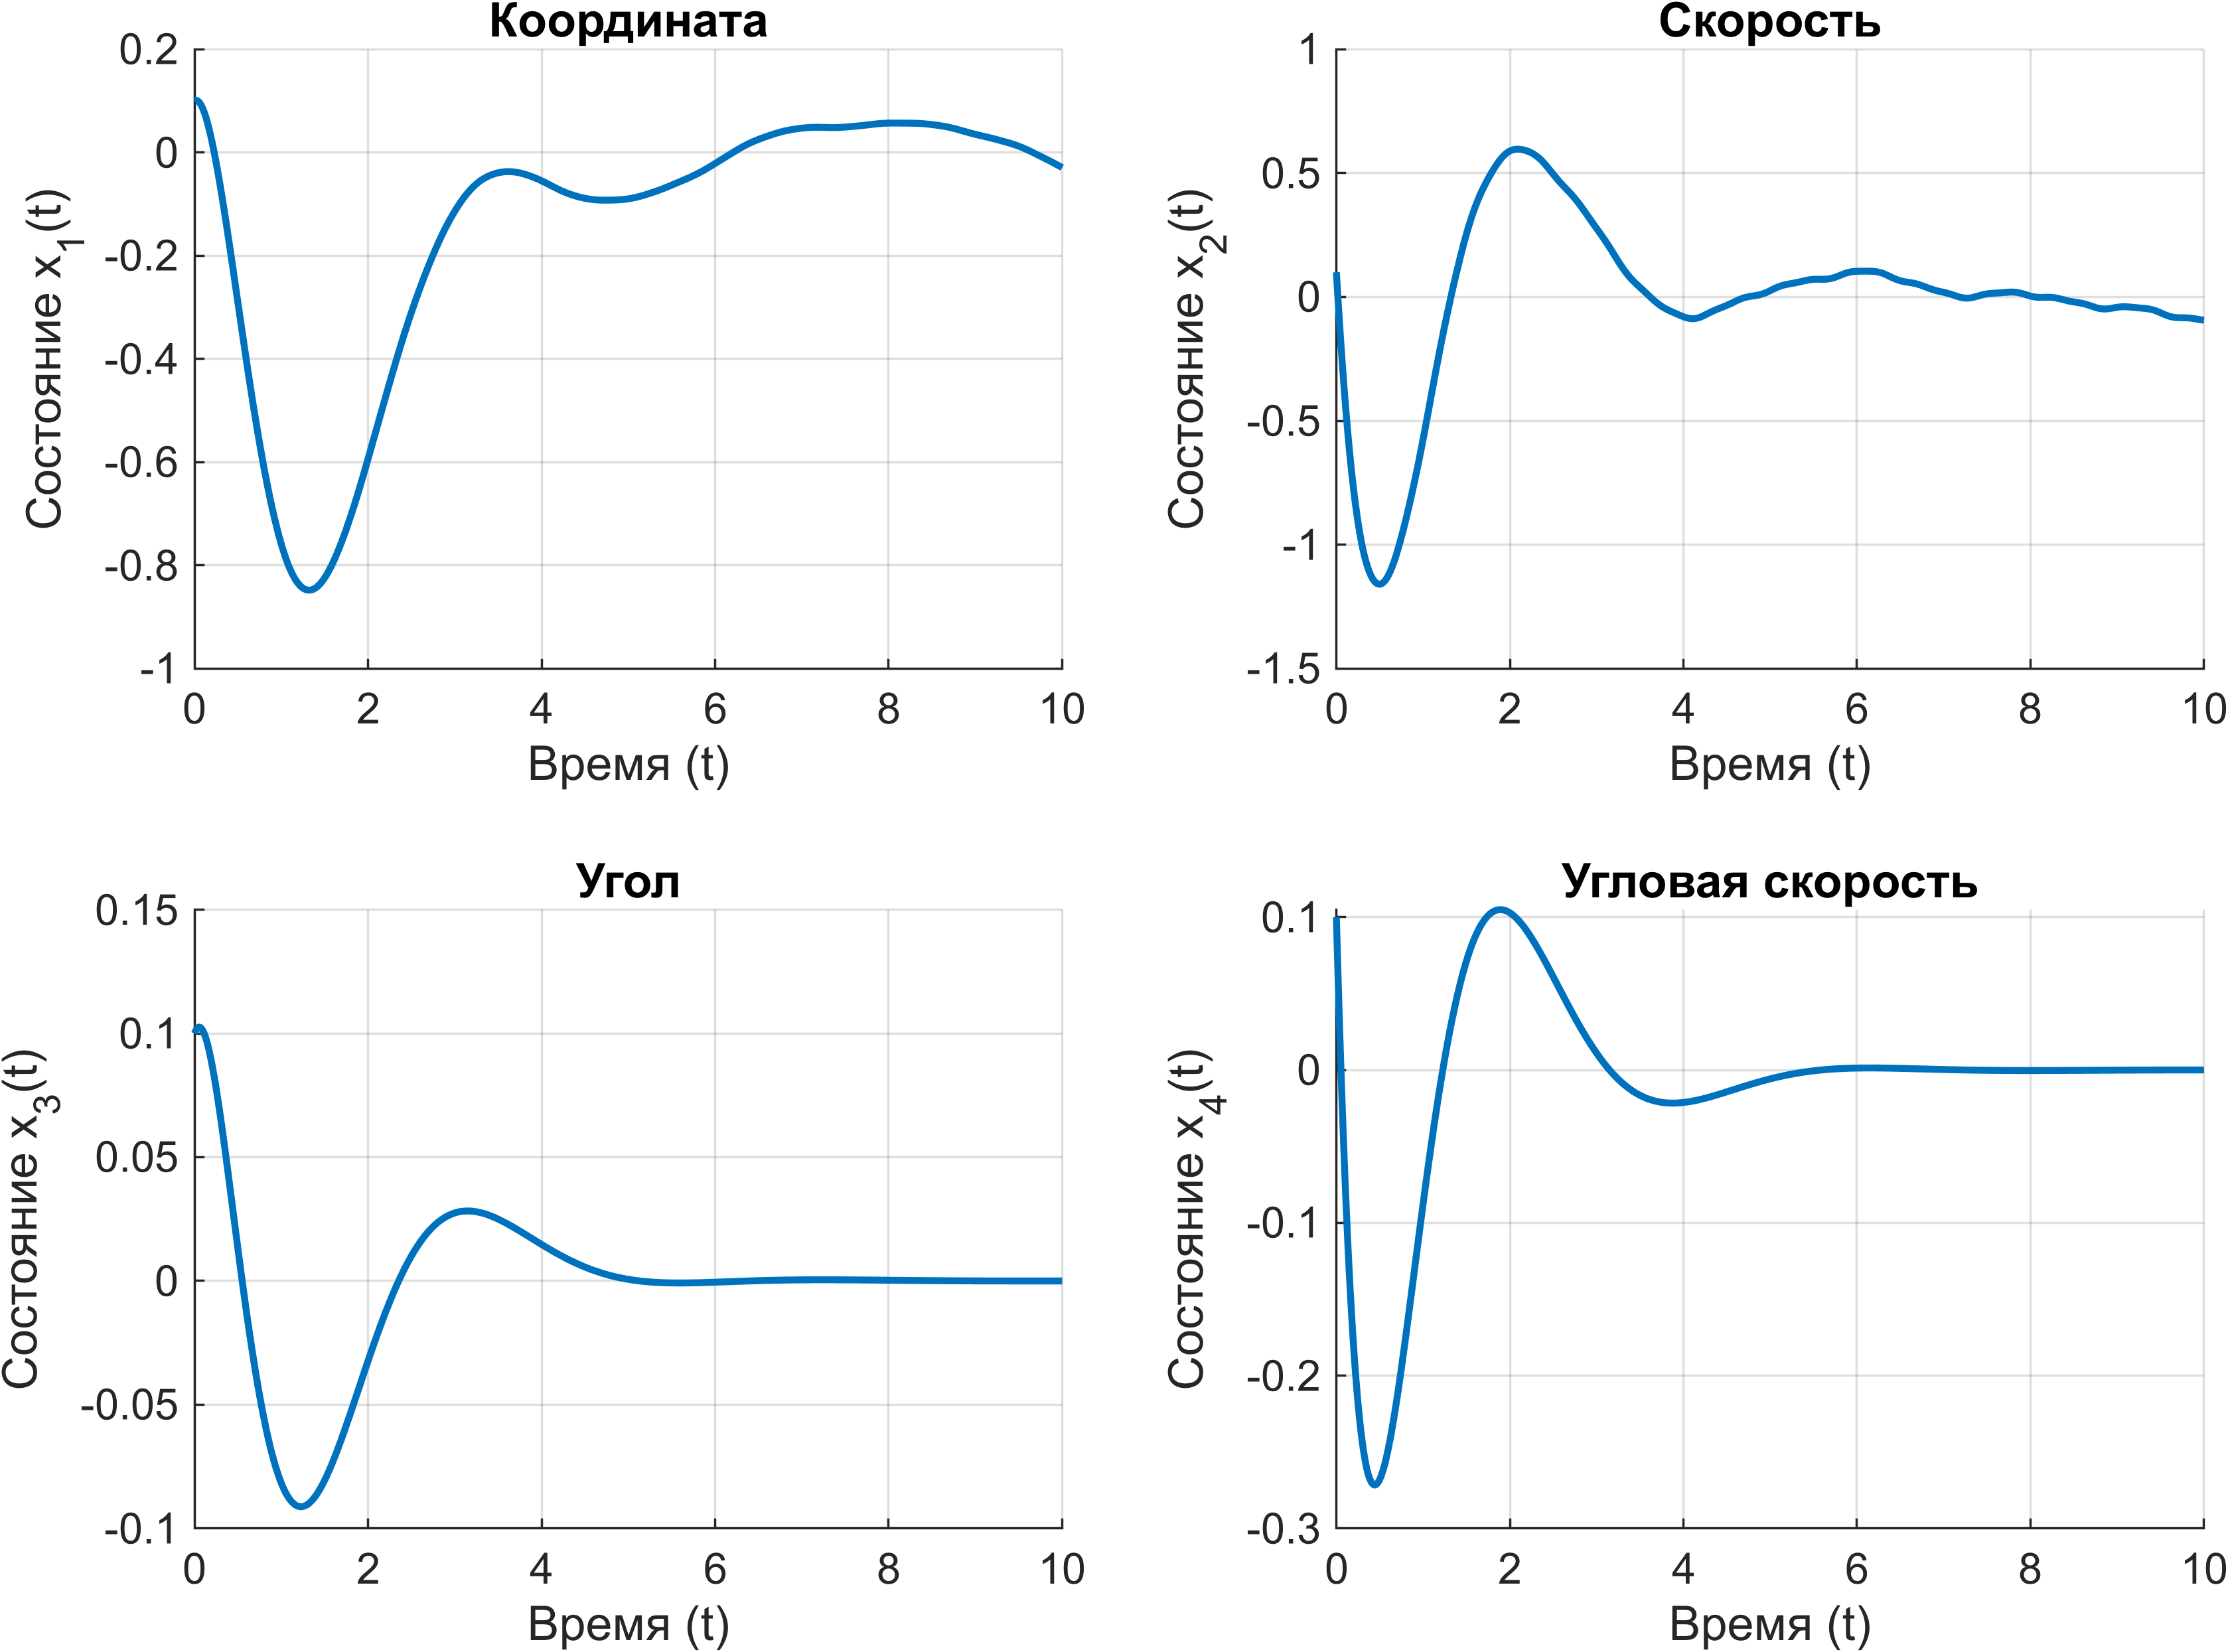
\includegraphics[width=\linewidth]{figs/5.1.lin.png}
    \caption{Моделирование работы компенсационного регулятора по состоянию
    линейной системы}
    \label{fig:5.1.lin}
\end{figure}
\begin{figure}[H]
    \centering
    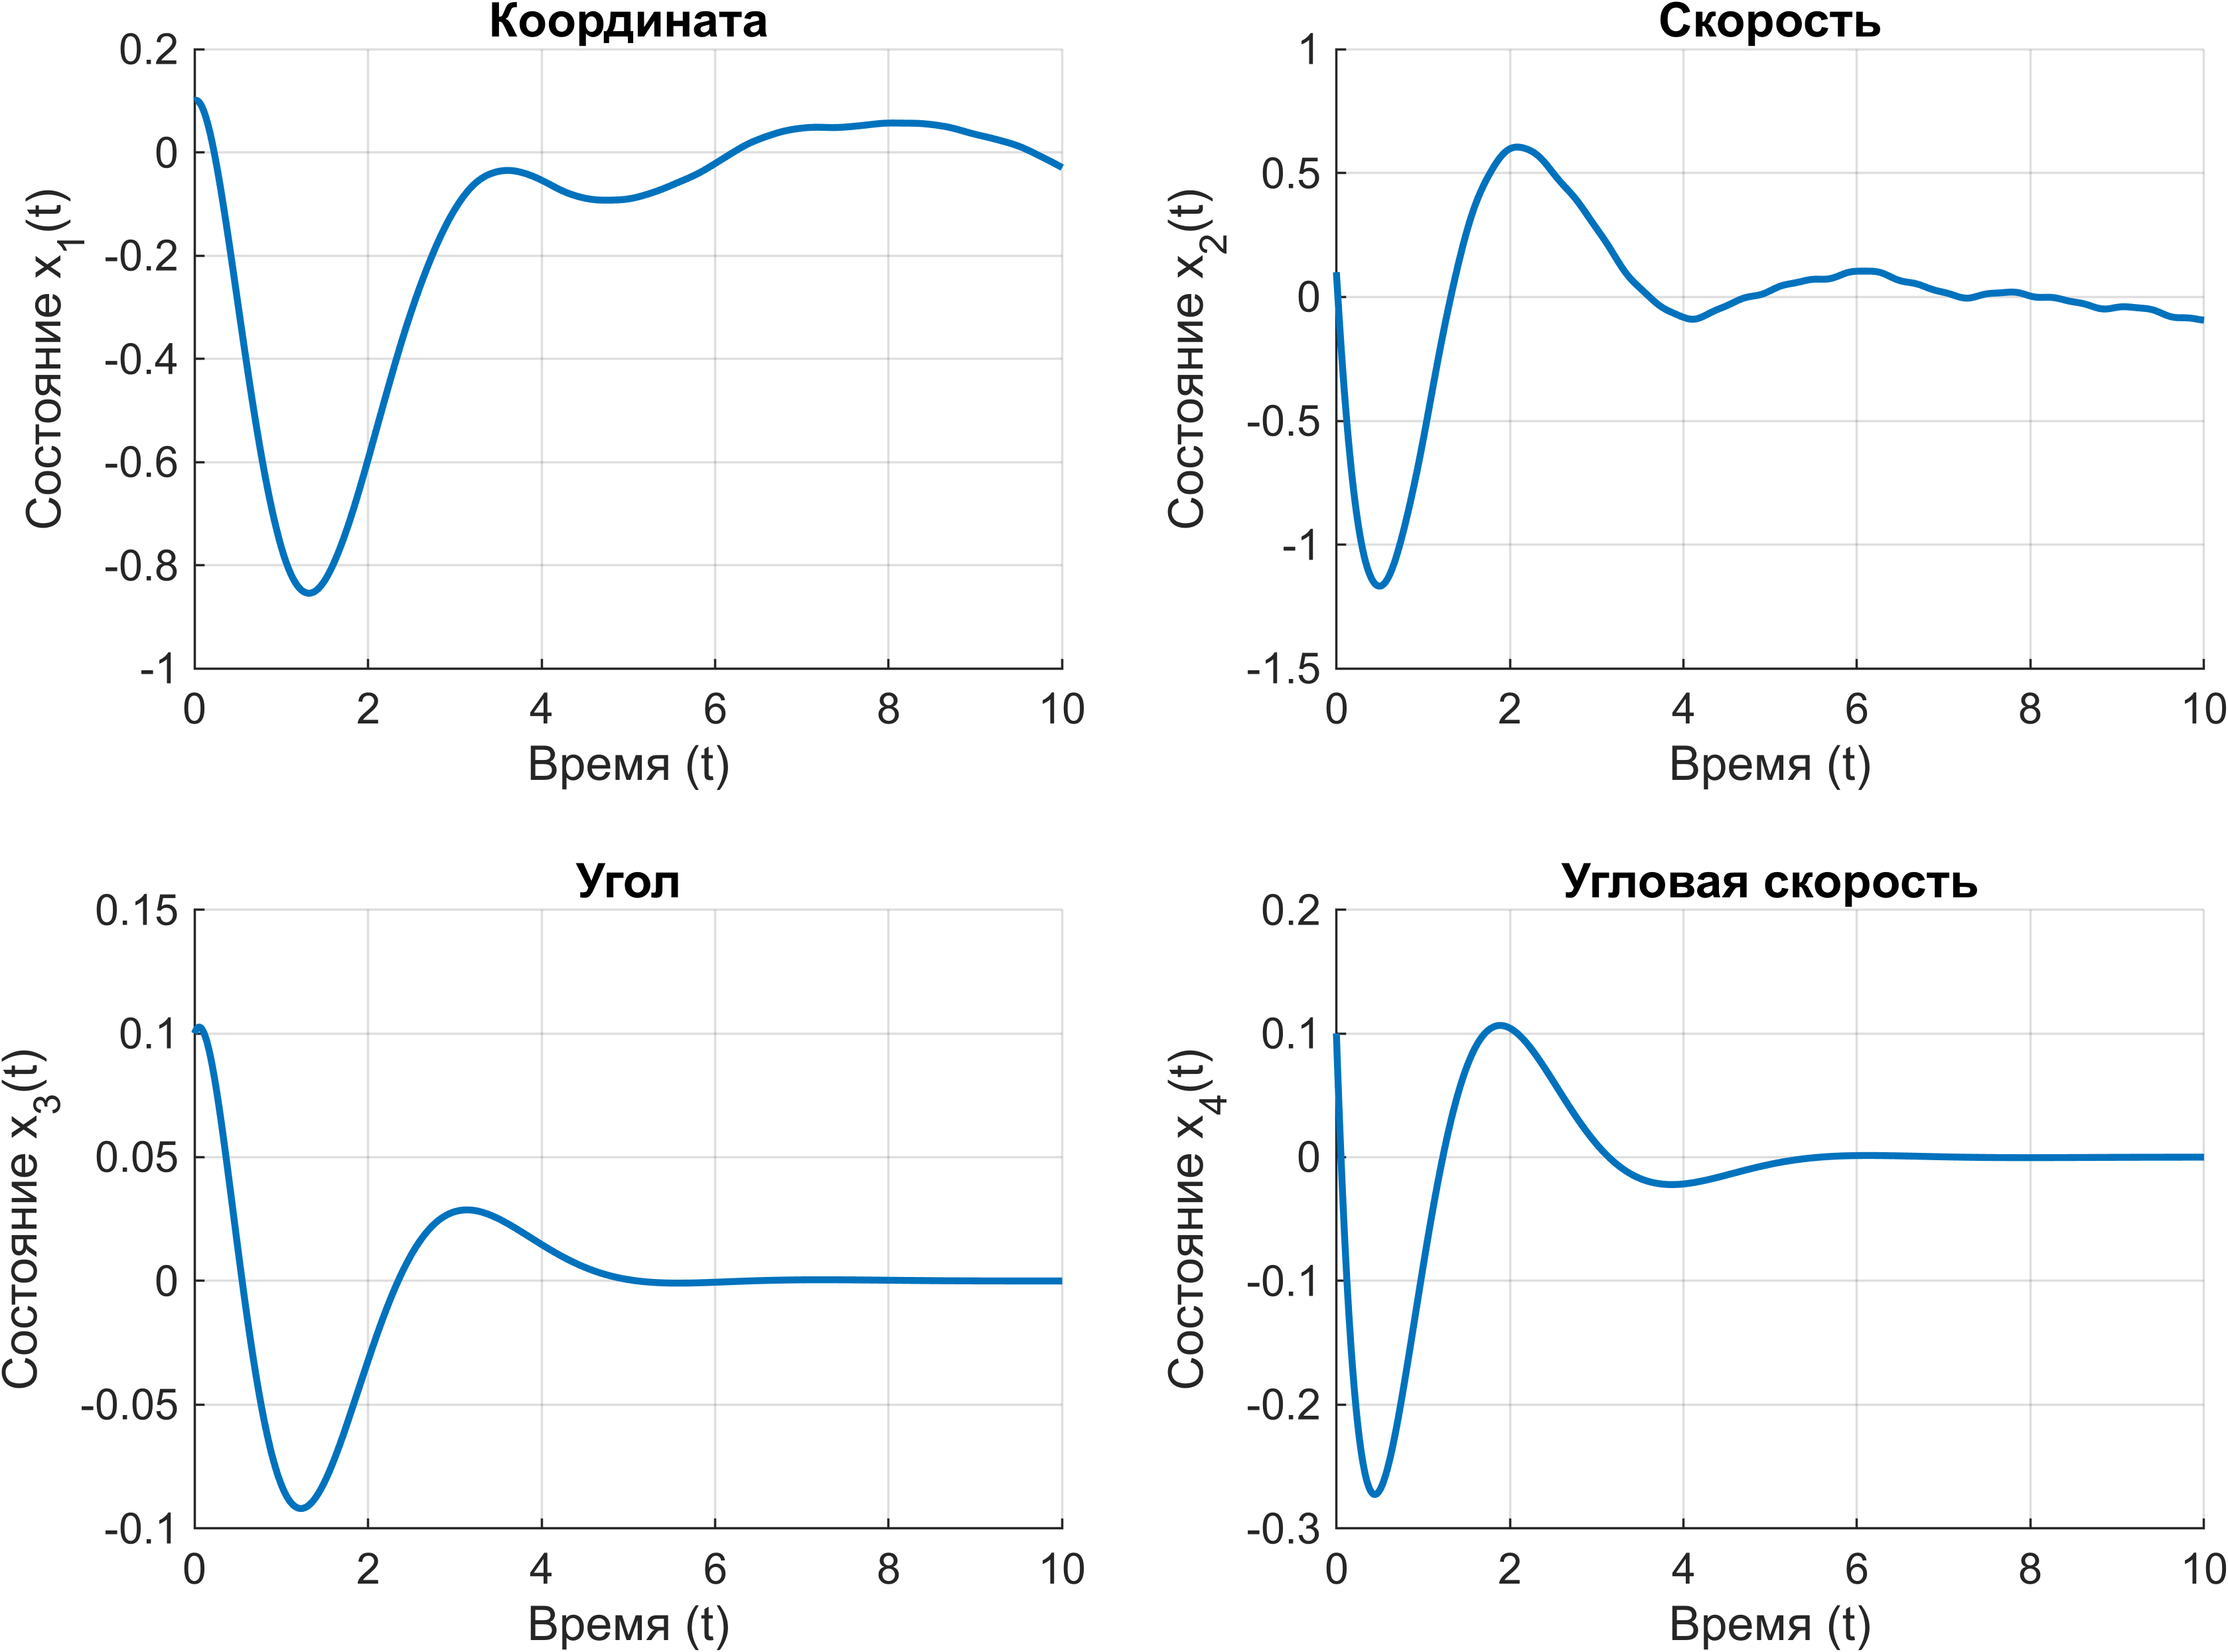
\includegraphics[width=\linewidth]{figs/5.1.nonlin.png}
    \caption{Моделирование работы компенсационного регулятора по состоянию
    нелинейной системы}
    \label{fig:5.1.nonlin}
\end{figure}

\section{Решение задачи слежения}

Положим $f \equiv 0$. Зададимся целевым сигналом
\begin{equation*}
    g(t)=0.1\sin(t)+0.19\sin(2t)+0.18\sin(3t)+0.17\sin(4t)+0.16\sin(5t),
\end{equation*}
тогда получаем следующий генератор:
\begin{equation}
    \label{eq:5.2.gen}
    \dot w_g=\Gamma_g w_g,\quad w_g(0),
\end{equation}
где
\begin{equation*}
    \Gamma_g=\begin{bmatrix}
0 & -1 & 0 & 0 & 0 & 0 & 0 & 0 & 0 & 0\\
1 & 0 & 0 & 0 & 0 & 0 & 0 & 0 & 0 & 0\\
0 & 0 & 0 & -2 & 0 & 0 & 0 & 0 & 0 & 0\\
0 & 0 & 2 & 0 & 0 & 0 & 0 & 0 & 0 & 0\\
0 & 0 & 0 & 0 & 0 & -3 & 0 & 0 & 0 & 0\\
0 & 0 & 0 & 0 & 3 & 0 & 0 & 0 & 0 & 0\\
0 & 0 & 0 & 0 & 0 & 0 & 0 & -4 & 0 & 0\\
0 & 0 & 0 & 0 & 0 & 0 & 4 & 0 & 0 & 0\\
0 & 0 & 0 & 0 & 0 & 0 & 0 & 0 & 0 & -5\\
0 & 0 & 0 & 0 & 0 & 0 & 0 & 0 & 5 & 0
     \end{bmatrix},\quad
        w_g(0)=\begin{bmatrix}
0\\
-0.1\\
0.09\\
0\\
0\\
-0.08\\
0.07\\
0\\
0\\
-0.06
        \end{bmatrix}.
\end{equation*}
Построим следящий регулятор, гарантирующий выполнение условия
\begin{equation}
    \label{eq:5.2.aim}
    \lim_{t \to \infty} \| \varphi(t) -g(t)\| = 0.
\end{equation}
Для этого составим регулируемый выход:
\begin{equation*}
    z=C_Zx,\quad C_Z=\begin{bmatrix}
        0 & 0 & 1 & 0
    \end{bmatrix},\quad
    D_Z=\begin{bmatrix}
        -1 & 0 & 0 & -1 & -1 & 0 & 0 & -1 & -1 & 0
    \end{bmatrix}.
\end{equation*}
Компенсирующий регулятор имеет следующий вид:
\begin{equation}
    \label{eq:5.2.reg}
    u=K_1x+K_2w_g.
\end{equation}
В качестве "feedback" компоненты используем \eqref{eq:4.4.K2}.
Для нахождения "feedforward" компоненты с помощью CVX решим следующую систему
\begin{equation*}
    \begin{cases}
        P\Gamma_g-AP=BY\\
        C_ZP+DZ=0
    \end{cases}
\end{equation*}
и получим
\begin{equation*}
    K_2=Y-K_1P=\begin{bmatrix}
4179.0 & 10550.0 & 3395.0 & 6624.0 & 2003.0 & -11900.0 & 19040.0 & -5609.0 & -15710.0 & -25640.0
    \end{bmatrix}
\end{equation*}
Моделирование линейной модели \eqref{eq:sys} можно увидеть на 
\autoref{fig:5.2.lin}. Нелинейной модели \eqref{eq:origsys} на
\autoref{fig:5.2.nonlin}. Графики очень похожи, но по ошибке слежения
видно, что нелинейная система справляется с задачей хуже, имея
периодические скачки, возможно, она и не выполнит целевое условие 
\eqref{eq:5.2.aim}, в любом случае, нелинейная система довольно хорошо
следует за $g(t)$, ведь колебания ошибки отклонения матрика имеют амплитуду 
всего около одного градуса.
\begin{figure}[H]
    \centering
    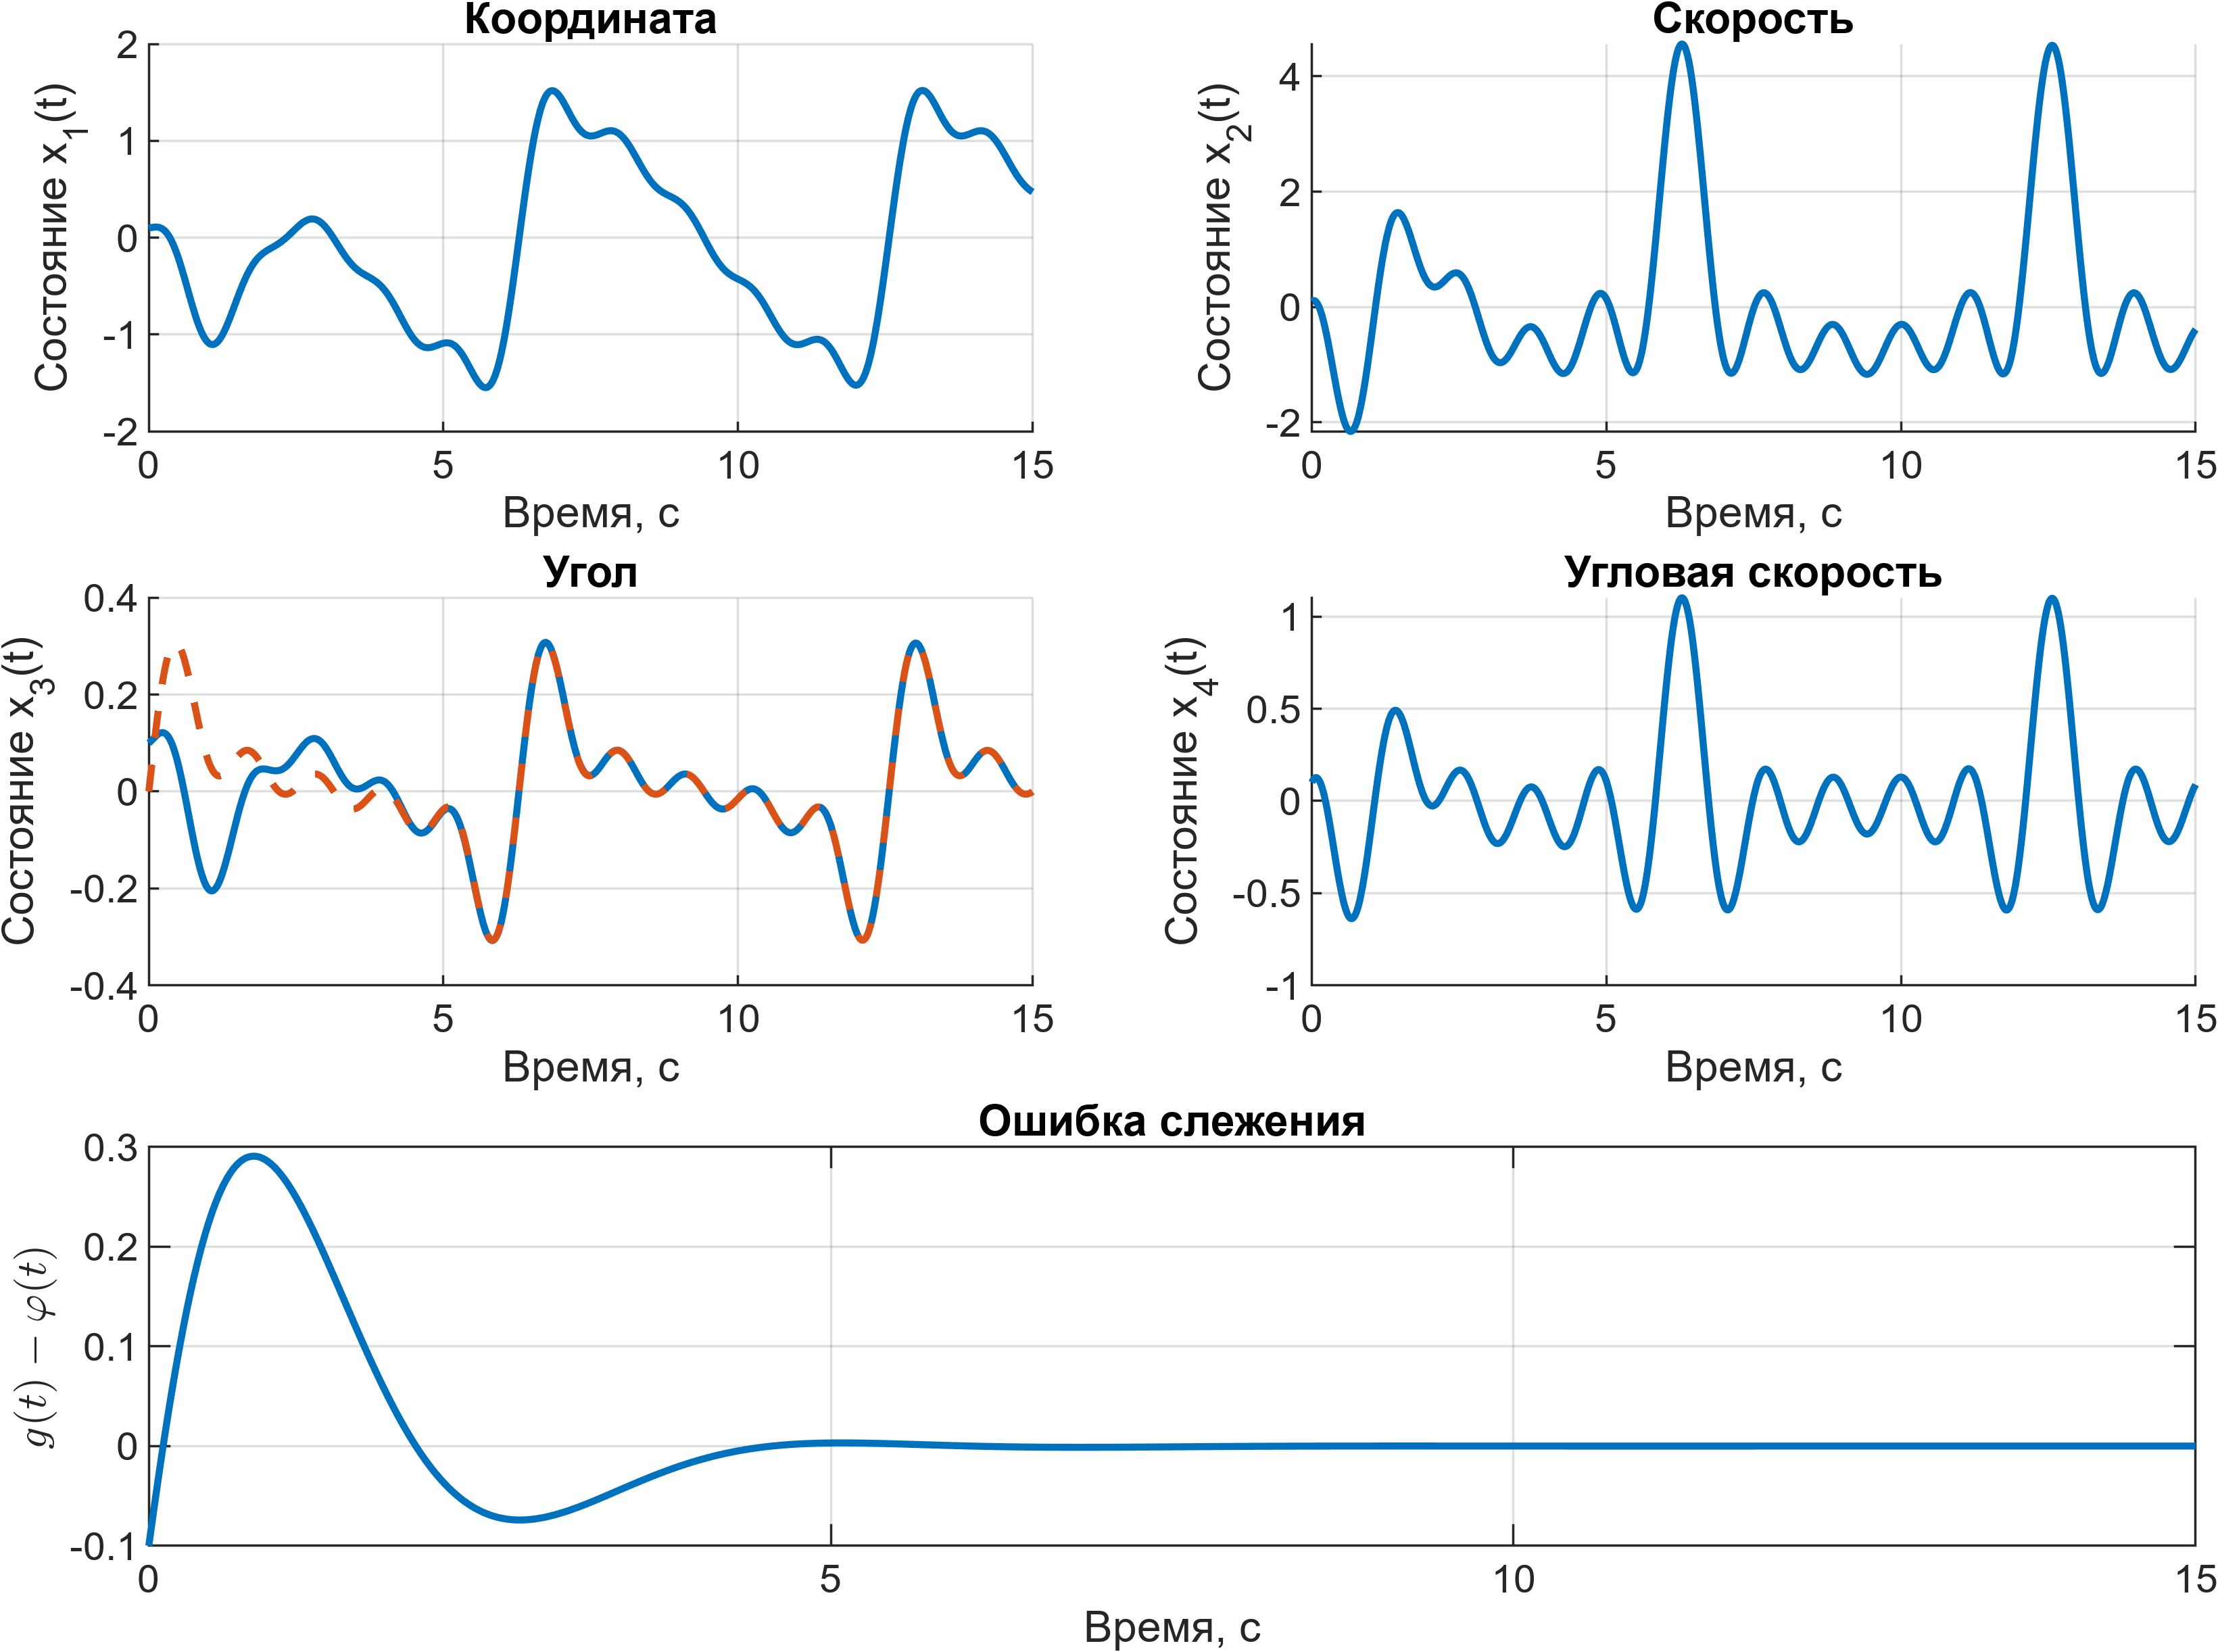
\includegraphics[width=\linewidth]{figs/5.2.lin.png}
    \caption{Моделирование работы компенсационного регулятора по состоянию
    линейной системы}
    \label{fig:5.2.lin}
\end{figure}
\begin{figure}[H]
    \centering
    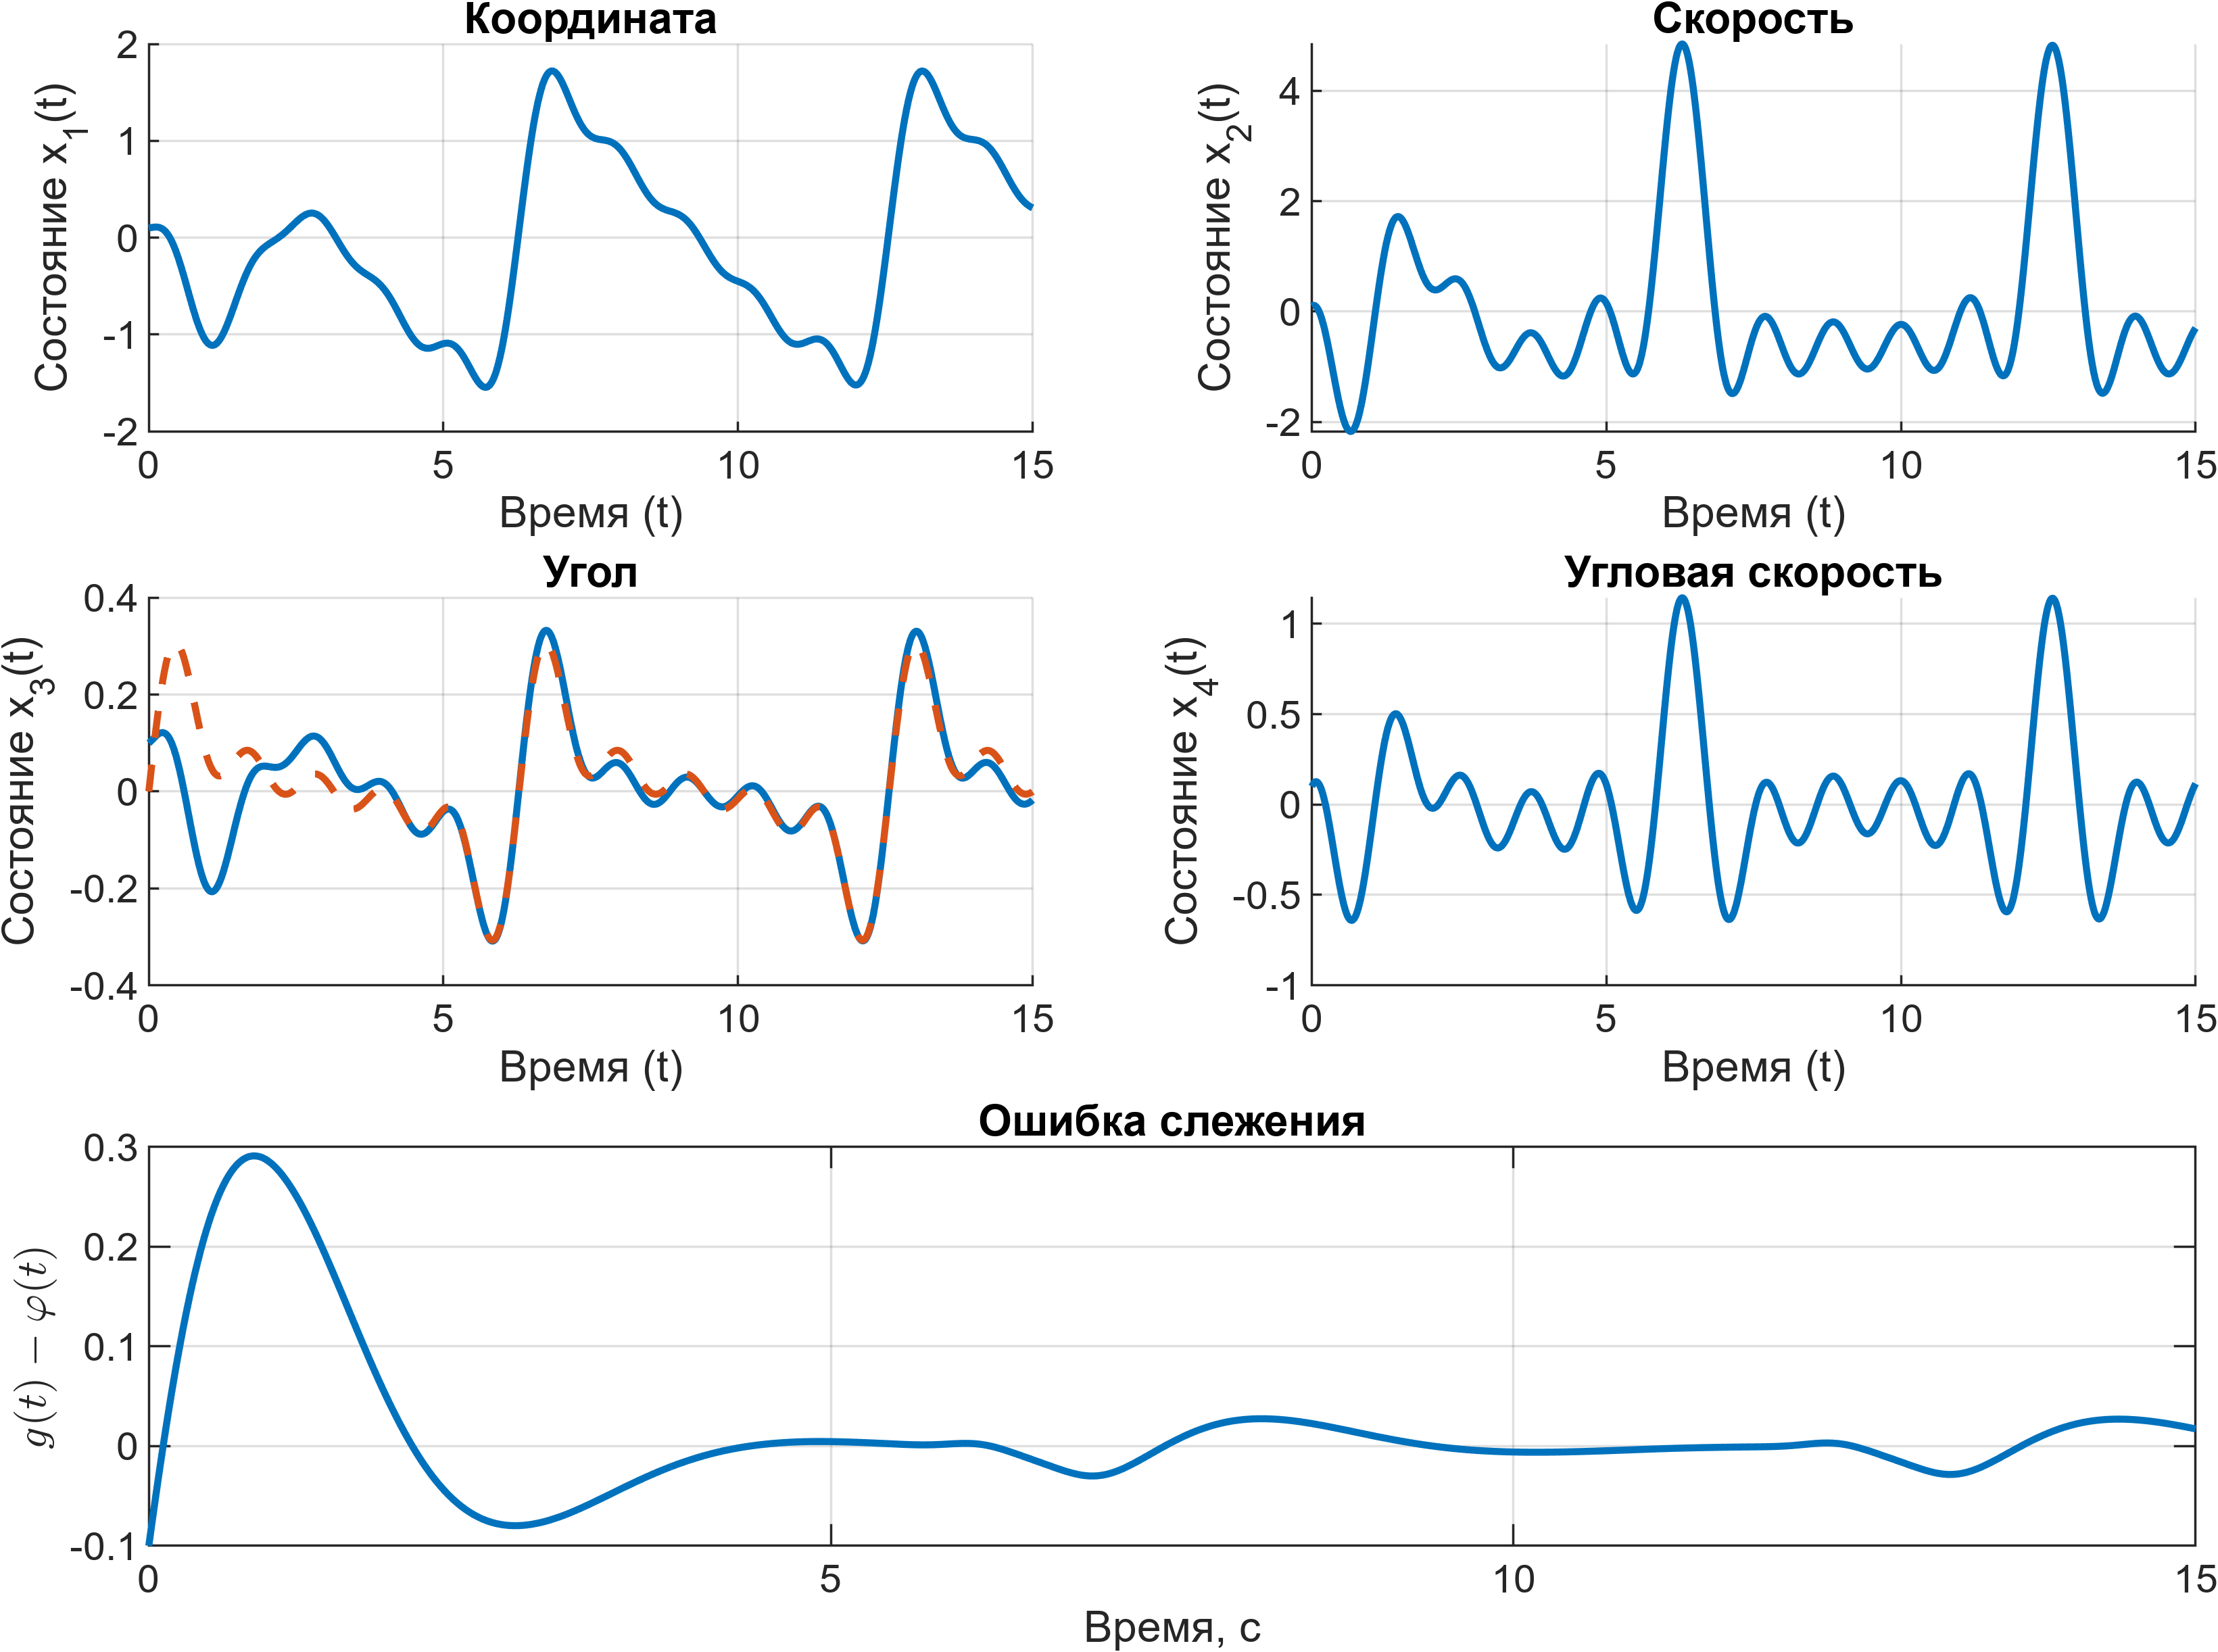
\includegraphics[width=\linewidth]{figs/5.2.nonlin.png}
    \caption{Моделирование работы компенсационного регулятора по состоянию
    нелинейной системы}
    \label{fig:5.2.nonlin}
\end{figure}
\noindent Нелинейная система может проследить не за любыми сигналами, например,
если взять условия для генератора сигнала слежения из генератора возмущения
предыдущего пункта, то, как видно на  \autoref{fig:5.2.nonlin.bad},
маятник упадет и не сможет вернуться обратно.
\begin{figure}[H]
    \centering
    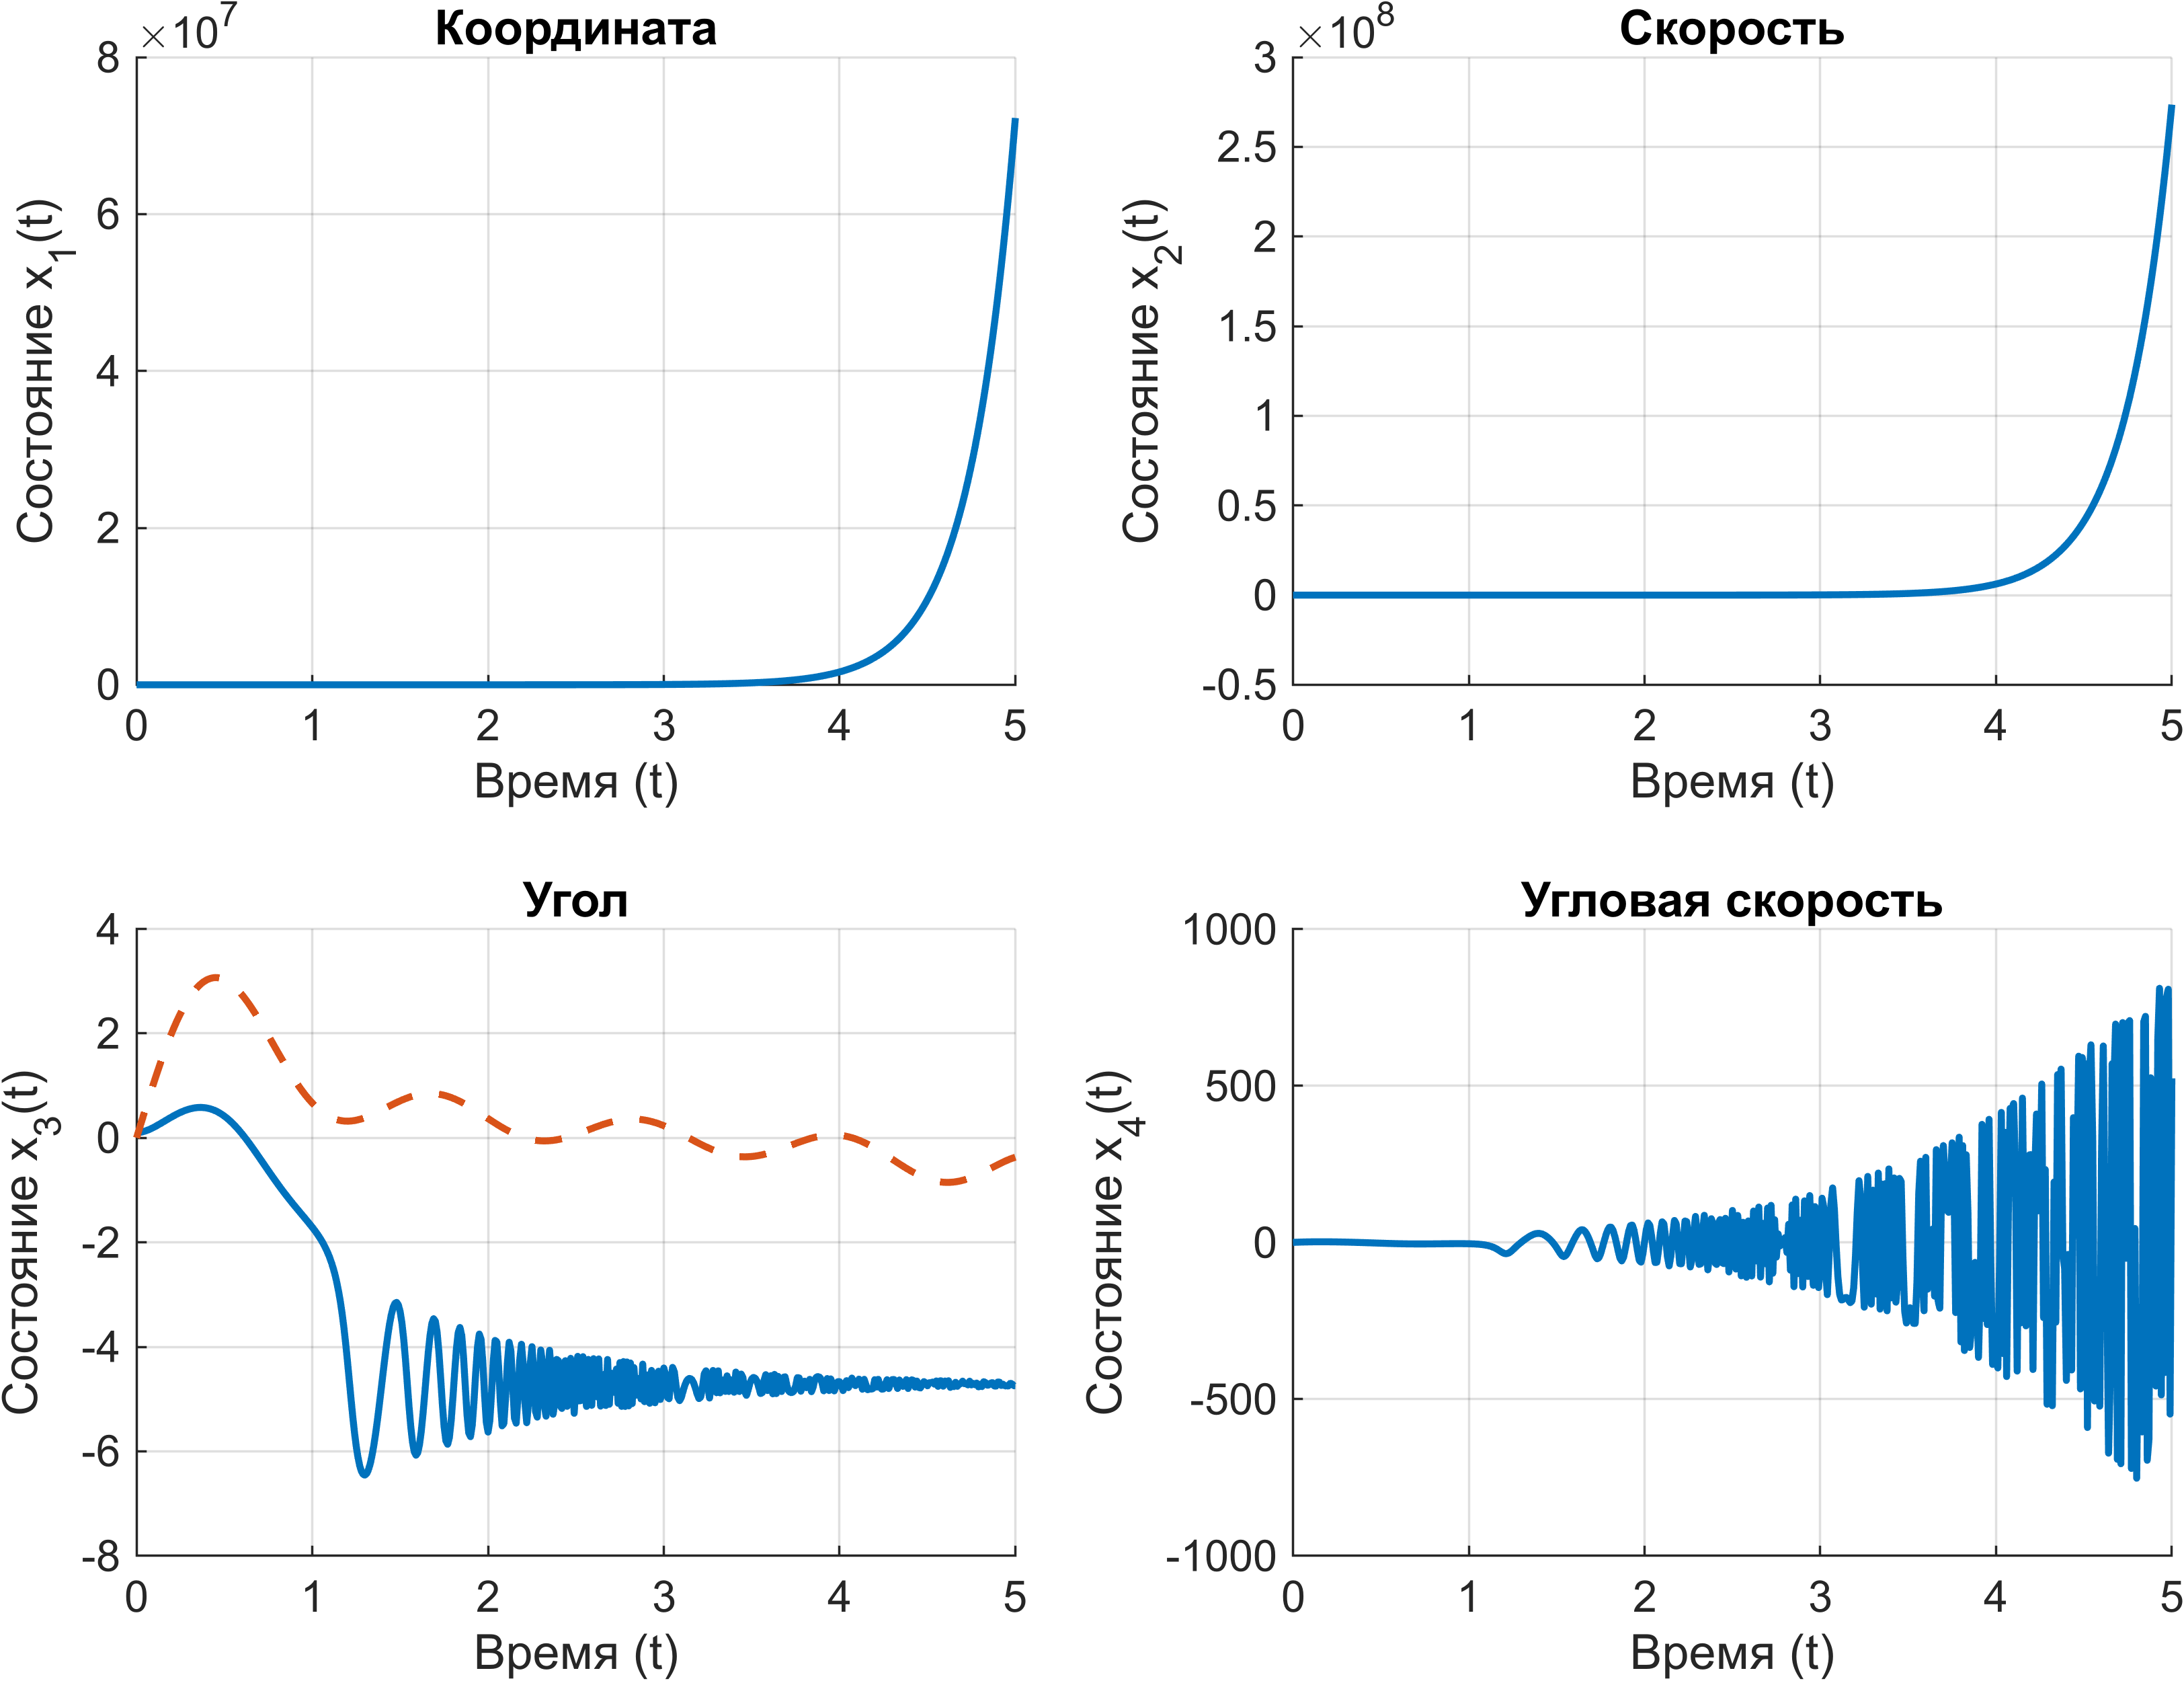
\includegraphics[width=\linewidth]{figs/5.2.nonlin.bad.png}
    \caption{Моделирование работы компенсационного регулятора по состоянию
    нелинейной системы с плохим сигналом для слежения}
    \label{fig:5.2.nonlin.bad}
\end{figure}

\chapter{Стабилизация маятника: LQR и фильтр Калмана}

\section{Синтез линейно-квадратичного регулятора}

Синтезируйте LQR-регулятор на основе линейной модели \eqref{eq:sys},
для выберем матрицы критерия качества:
\begin{equation*}
    Q=\begin{bmatrix}
        100&0&0&0\\
        0&100&0&0\\
        0&0&100&0\\
        0&0&0&100
    \end{bmatrix},\quad
    R=1,
\end{equation*}
таким выбором элементов матриц регулятор будет минимизировать состояние
не взирая на затраты на управление.
С помощью icare найдем решение уравнения Риккати:
\begin{equation*}
    A^TP+PA+Q-PBR^{-1}B^TP=0,
\end{equation*}
и вычислим матрицу регулятора:
\begin{equation*}
    K=-R^{-1}B^TP=\begin{bmatrix}
10.0 & 109.7 & -10720.0 & -5198.0
    \end{bmatrix}.
\end{equation*}
Спектр замкнутой системы получился следующий
\begin{equation*}
    \sigma(A+BK)=\begin{bmatrix}
-2.067&
-2.0593&
-0.10097\pm0.099951\,\mathrm{i}
    \end{bmatrix},
\end{equation*}
регулятор ситезирован успешно.
Применим его для управления нелинейной системой \eqref{eq:origsys} и
исследуем работоспособность в зависимости от начальных условий.
\begin{equation*}
    x_{01}=\begin{bmatrix}
        563\\
        0.1\\
        0.1\\
        0.1
    \end{bmatrix},\quad
    x_{02}=\begin{bmatrix}
        0.1\\
        45\\
        0.1\\
        0.1
    \end{bmatrix},\quad
    x_{03}=\begin{bmatrix}
        0.1\\
        0.1\\
        1.2\\
        0.1
    \end{bmatrix},\quad
    x_{04}=\begin{bmatrix}
        0.1\\
        0.1\\
        0.1\\
        5
    \end{bmatrix},
\end{equation*}
при значениях больше, система не сойдется к положению неустойчивого равновесия.
Графики состояния можно увидеть на \autoref{fig:6.1.sim}. Система успешно
стаблизирует маятник в верхнем положении. По сравнению с модальным регулятором,
регулятором с заданной степенью устойчивости начальные условия гораздо шире:
\begin{itemize}
    \item Максимальное положение тележки: $563$ м,
    \item Максимальная скорость тележки: $45$ м/с,
    \item Максимальный угол отклонения маятника: $68.8^\circ$,
    \item Максимальная угловая скорость маятника: $286.6^\circ$/с.
    \end{itemize}
\begin{figure}[H]
    \centering
    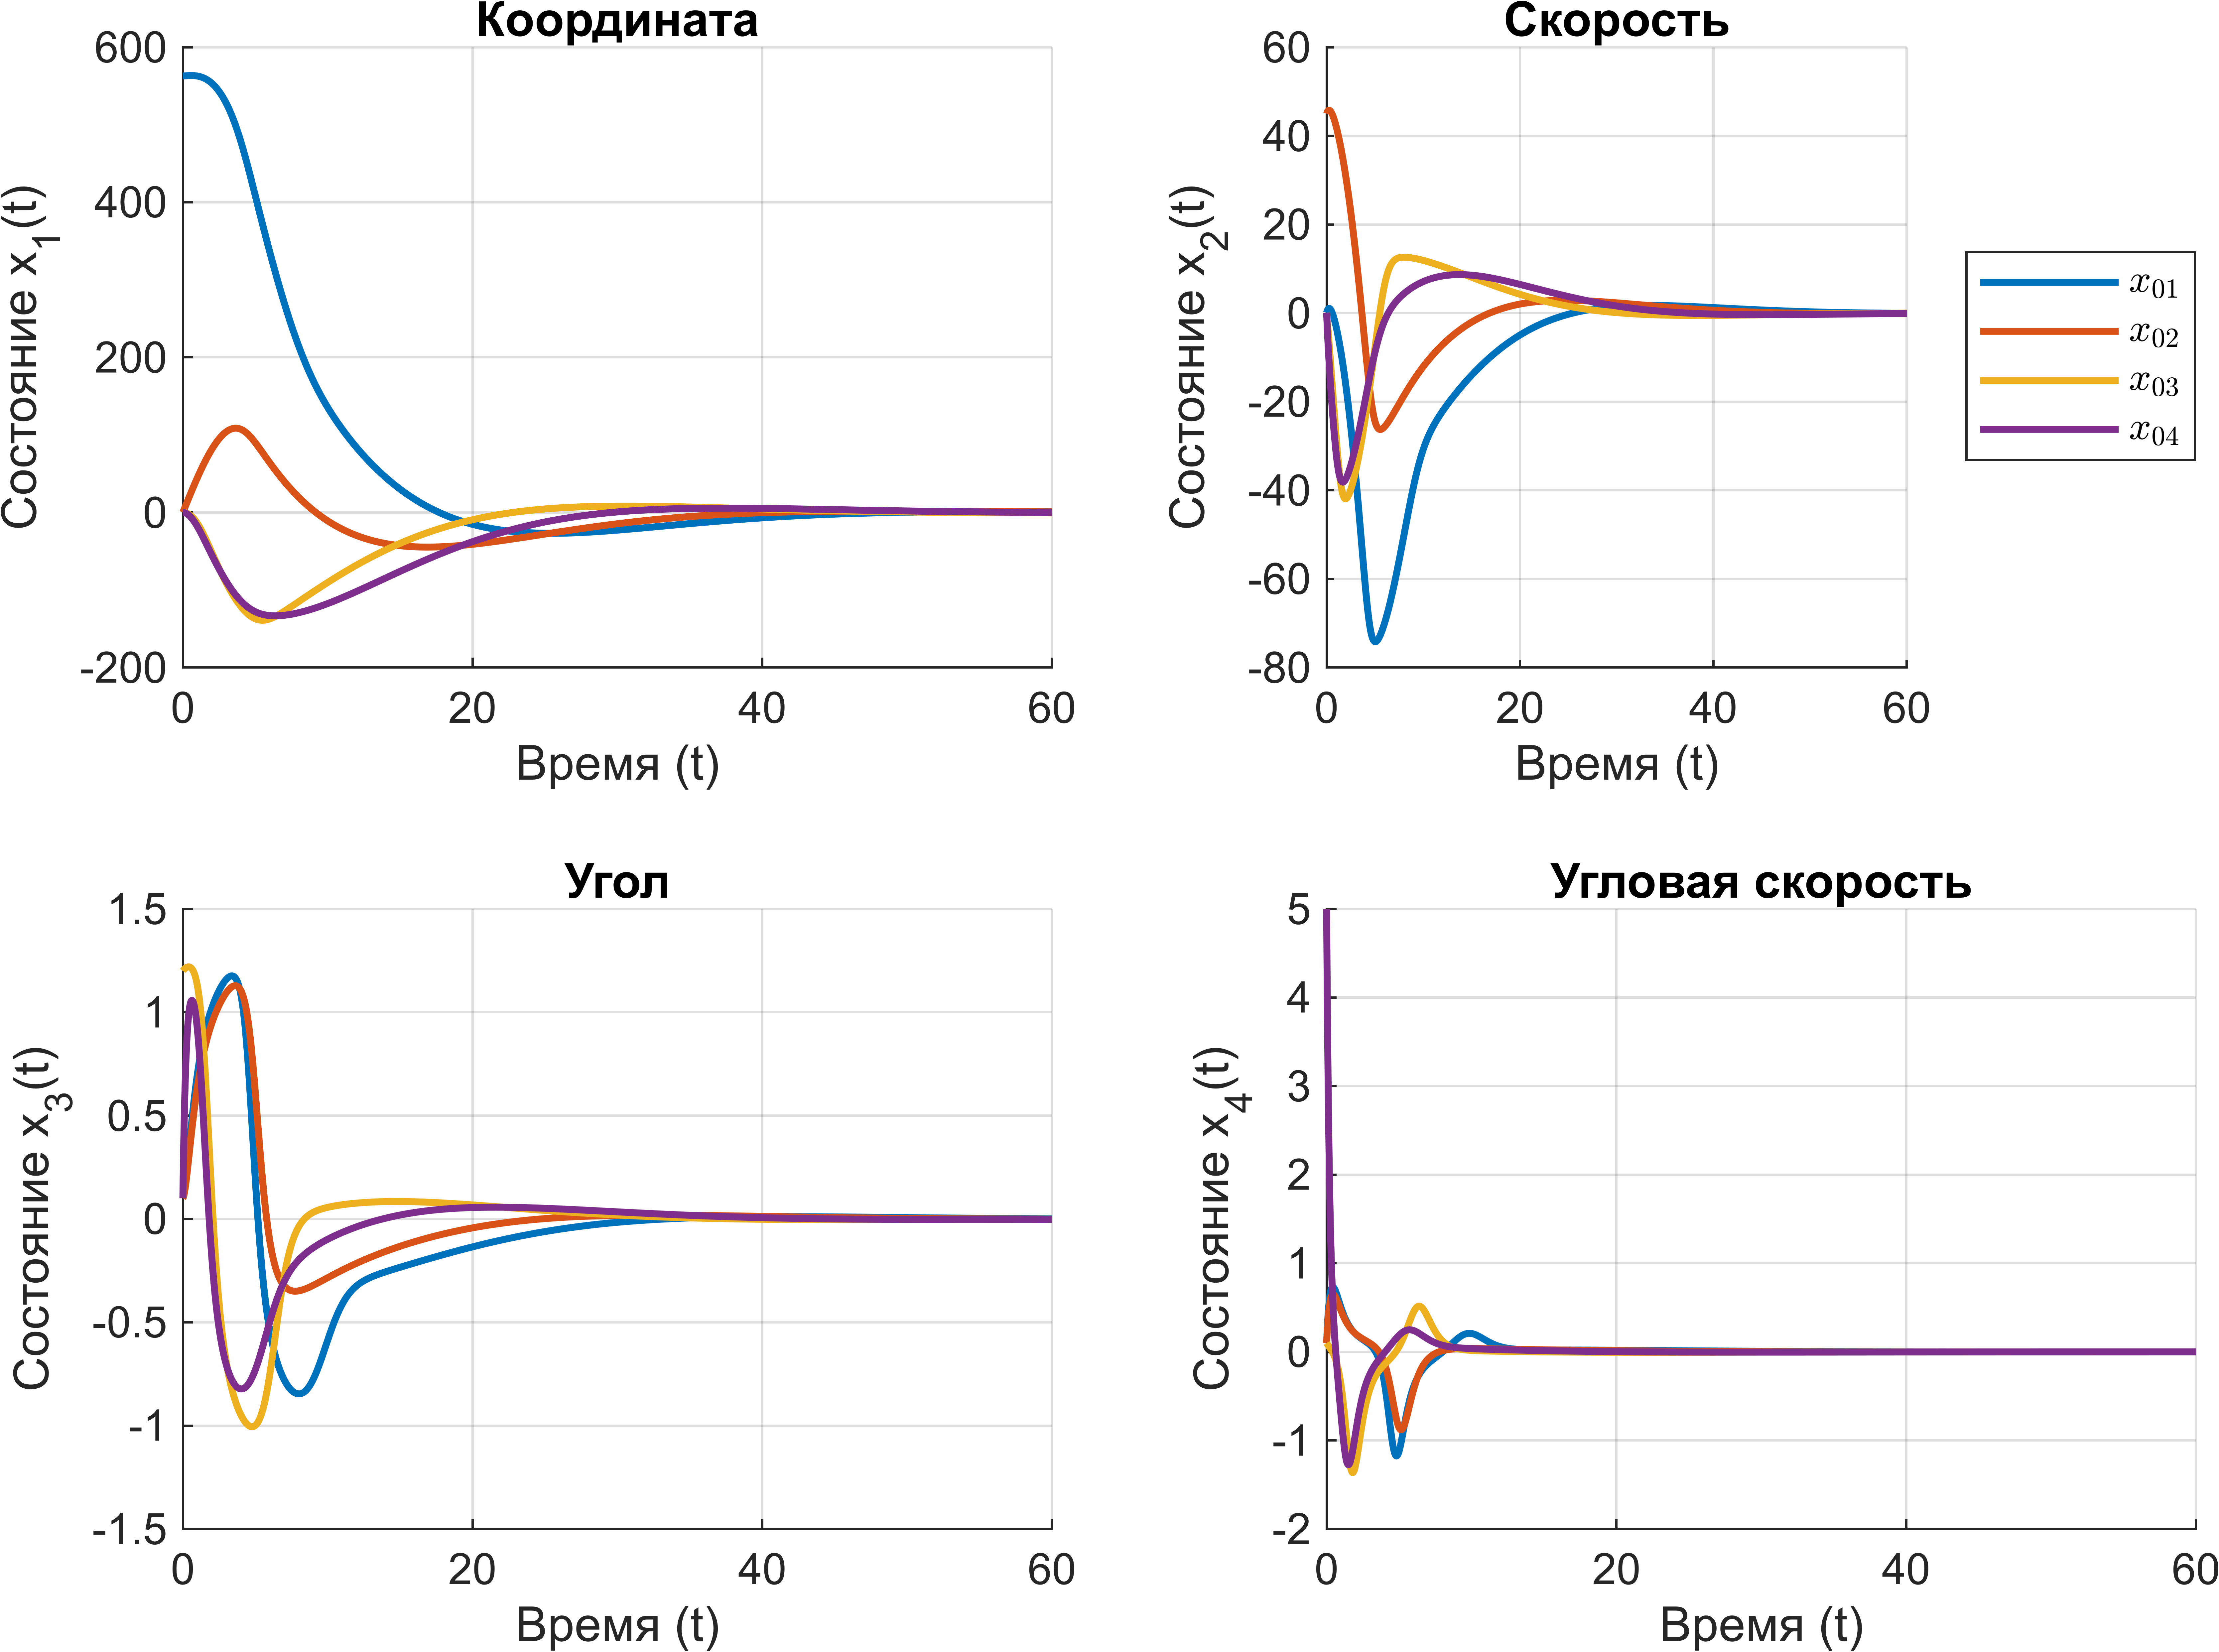
\includegraphics[width=\linewidth]{figs/6.1.sim.png}
    \caption{Моделирование работы LQR-регулятора при устойчивых 
    начальных условиях}
    \label{fig:6.1.sim}
\end{figure}
Возьмем немного большие начальные условия:
\begin{equation*}
    x_{01}=\begin{bmatrix}
        564\\
        0.1\\
        0.1\\
        0.1
    \end{bmatrix},\quad
    x_{02}=\begin{bmatrix}
        0.1\\
        46\\
        0.1\\
        0.1
    \end{bmatrix},\quad
    x_{03}=\begin{bmatrix}
        0.1\\
        0.1\\
        1.3\\
        0.1
    \end{bmatrix},\quad
    x_{04}=\begin{bmatrix}
        0.1\\
        0.1\\
        0.1\\
        6
    \end{bmatrix},
\end{equation*}
чтобы продемонстрировать плохие начальные условия.
Графики состояния можно увидеть на \autoref{fig:6.1.sim.bad}.
Поведение системы очень отличается от таковой с модальным регулятором,
маятник не устанавливает в одном их горизонтальных положений, а продолжиельно
колеблется с постоянной амплитудой, координата не расходится бесконечно,
а устанавливается на какой-то координате, за исключением $x_{04}$.
\begin{figure}[H]
    \centering
    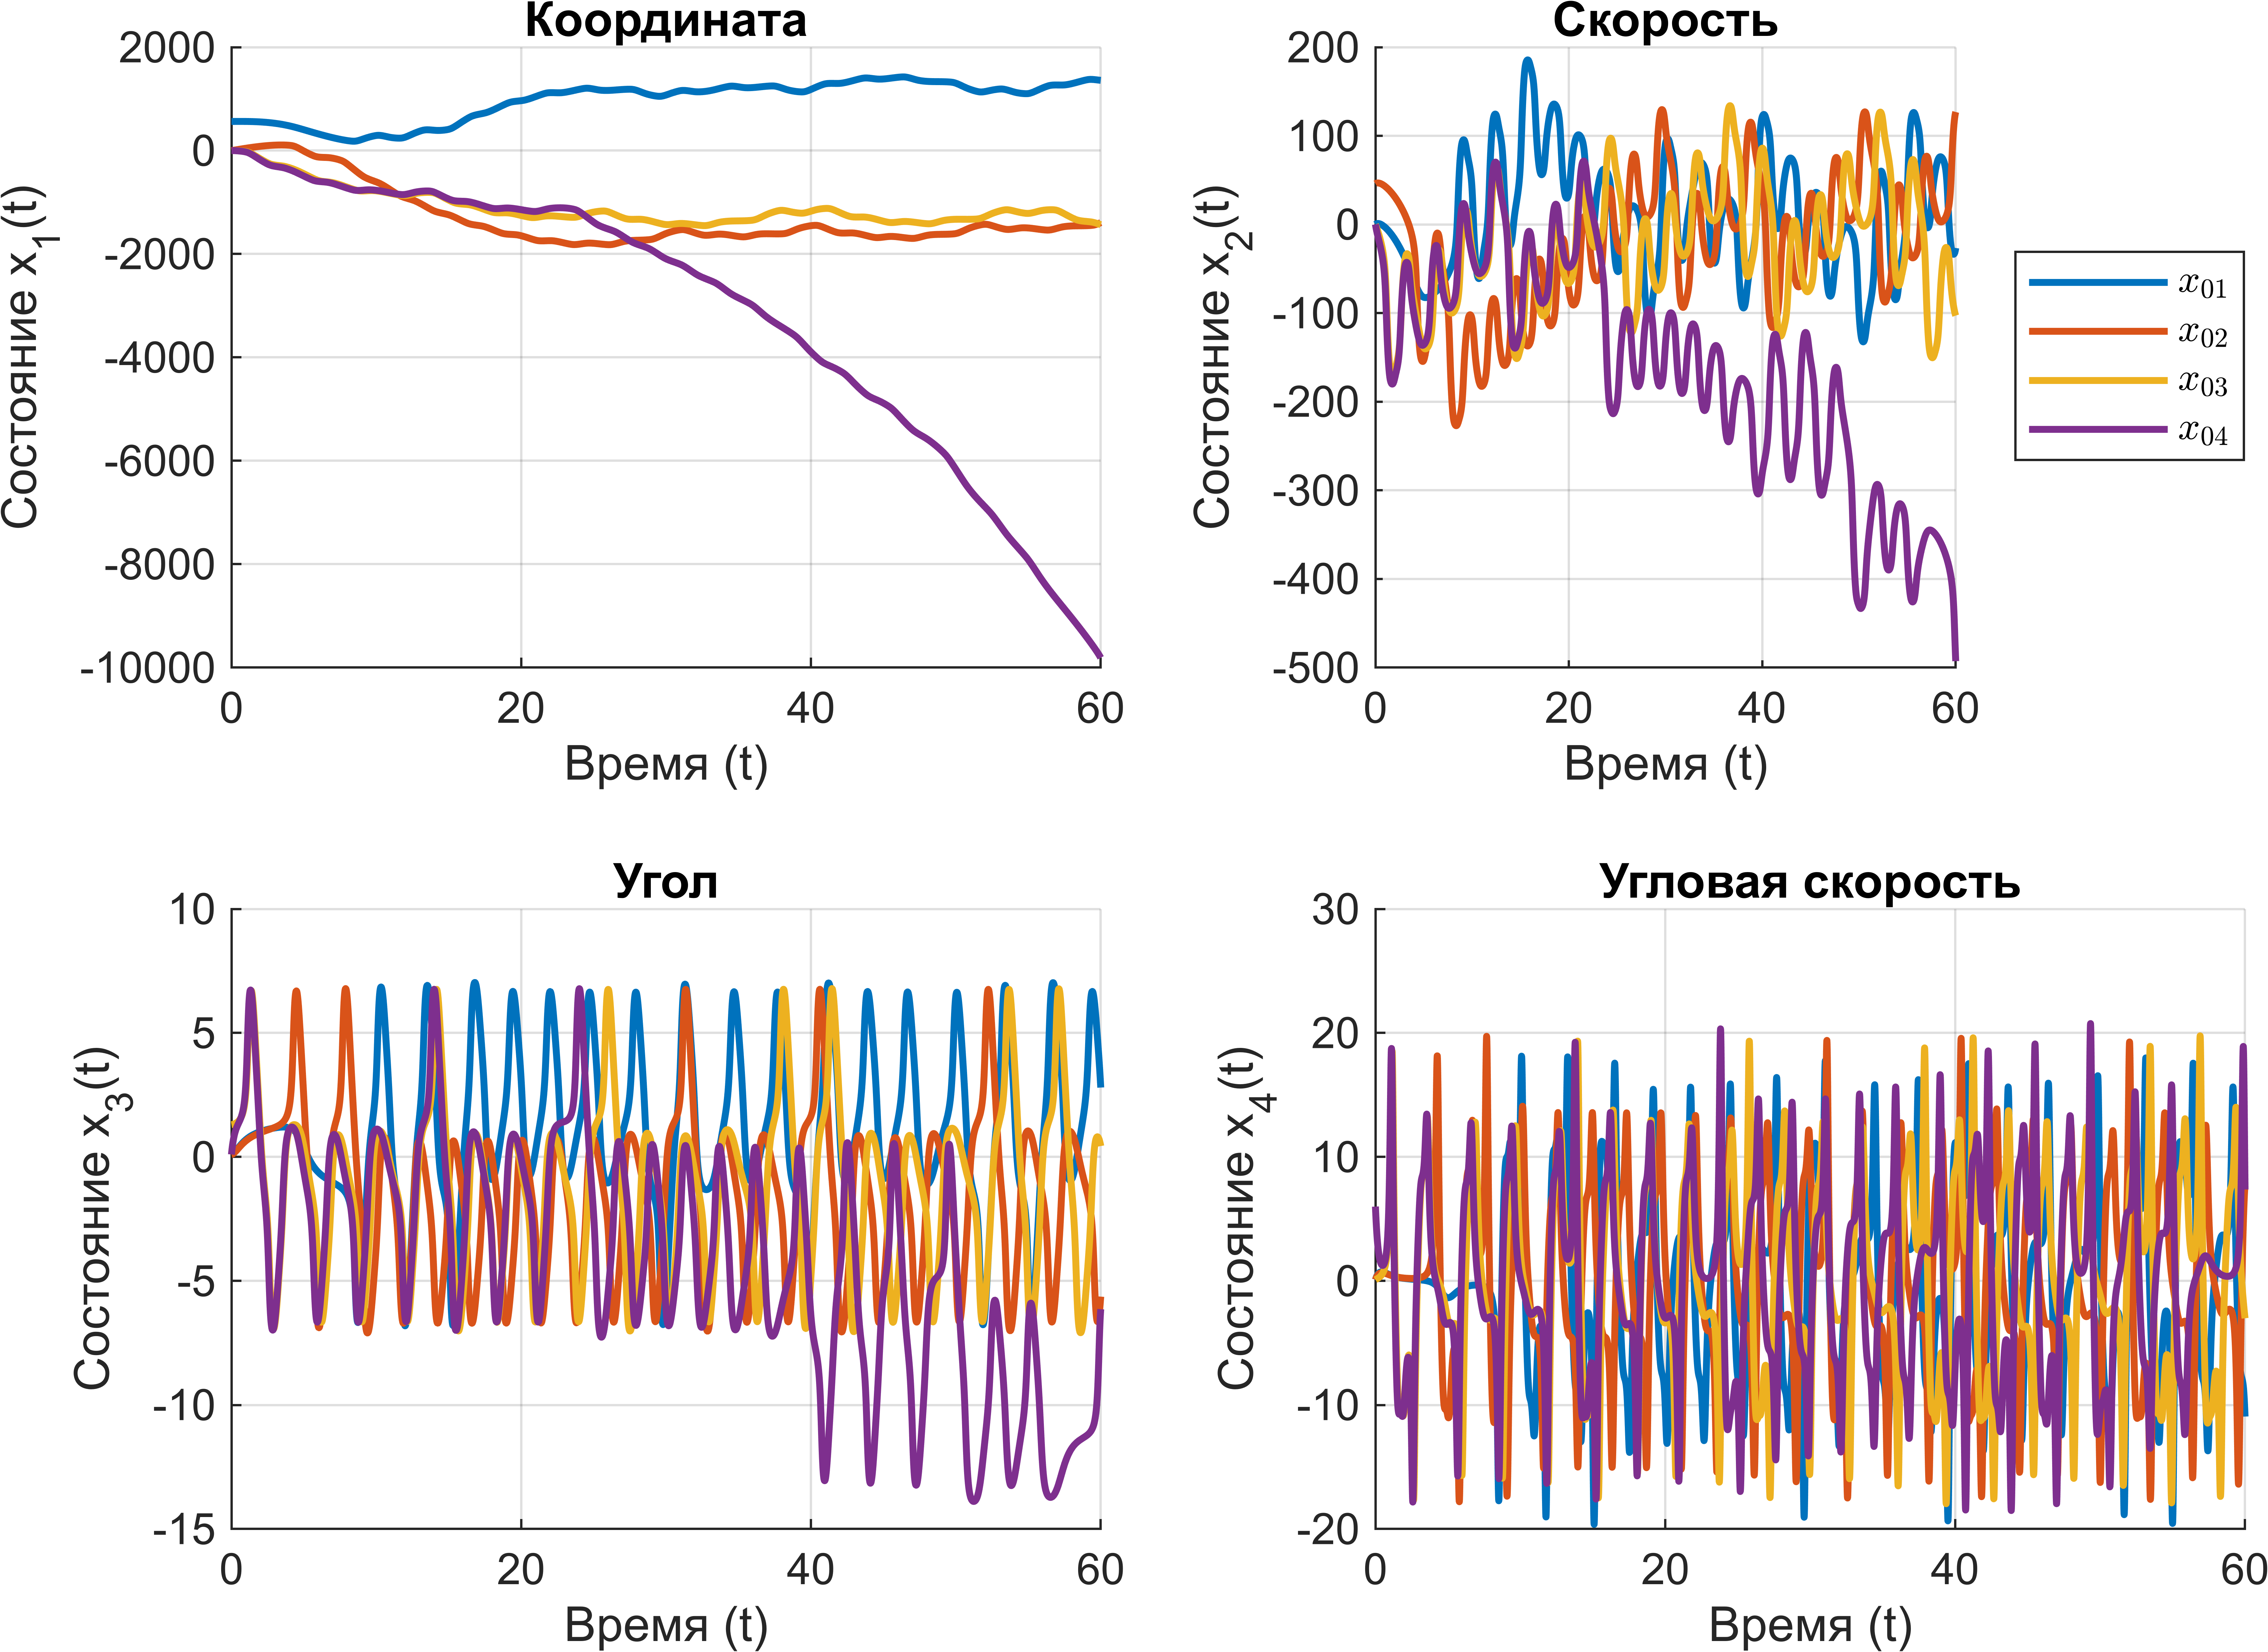
\includegraphics[width=\linewidth]{figs/6.1.sim.bad.png}
    \caption{Моделирование работы LQR-регулятора при неустойчивых 
    начальных условиях}
    \label{fig:6.1.sim.bad}
\end{figure}

\section{Исследование линейно-квадратичного регулятора}

Исследуем влияние весовых матриц LQR-регулятора на максимальное отклонение 
маятника от вертикали, максимальное горизонтальное смещение тележки и 
максимальное значение управляющего сигнала при управлении нелинейной 
системой \eqref{eq:origsys}. Выьерем начальные условия на $0.1$.
Так как для весовых матриц важно соотношение их чисел, зафиксируем матрицу
$R=1$ и будем менять $Q$, рассмотрим четыре матрицы:
\begin{gather*}
Q_1 = \begin{bmatrix}
100 & 0 & 0 & 0 \\
0 & 100 & 0 & 0 \\
0 & 0 & 100 & 0 \\
0 & 0 & 0 & 100
\end{bmatrix},\quad
Q_2 = \begin{bmatrix}
100 & 0 & 0 & 0 \\
0 & 1 & 0 & 0 \\
0 & 0 & 1 & 0 \\
0 & 0 & 0 & 1
\end{bmatrix},\\
Q_3 = \begin{bmatrix}
1 & 0 & 0 & 0 \\
0 & 1 & 0 & 0 \\
0 & 0 & 100 & 0 \\
0 & 0 & 0 & 1
\end{bmatrix},\quad
Q_4 = \begin{bmatrix}
0.01 & 0 & 0 & 0 \\
0 & 0.01 & 0 & 0 \\
0 & 0 & 0.01 & 0 \\
0 & 0 & 0 & 0.01
\end{bmatrix},
\end{gather*}
четыре регулятора будут "стараться" минимизировать все состояние, координату
тележки, угол маятника и управление соответственно. Получились следующие матрицы
\begin{equation*}
\renewcommand{\arraystretch}{1.2}
\begin{array}{ll}
K_1 = \begin{bmatrix} 10.0 & 109.7 & -10720.0 & -5198.0 \end{bmatrix}, &
\sigma_1 = \begin{Bmatrix}
-2.067\\
-2.0593\\
-0.10097 \pm 0.09995\,\mathrm{i}
\end{Bmatrix} \\[3ex]
K_2 = \begin{bmatrix} 10.0 & 109.2 & -10710.0 & -5196.0 \end{bmatrix}, &
\sigma_2 = \begin{Bmatrix}
-2.0635\\
-2.0628\\
-0.10047 \pm 0.10045\,\mathrm{i}
\end{Bmatrix} \\[3ex]
K_3 = \begin{bmatrix} 1.0 & 32.46 & -10020.0 & -4860.0 \end{bmatrix}, &
\sigma_3 = \begin{Bmatrix}
-2.0632 \pm 0.00208\,\mathrm{i}\\
-0.03179 \pm 0.03175\,\mathrm{i}
\end{Bmatrix} \\[3ex]
K_4 = \begin{bmatrix} 0.1 & 10.05 & -9815.0 & -4758.0 \end{bmatrix}, &
\sigma_4 = \begin{Bmatrix}
-2.0632\\
-2.0631\\
-0.01005 \pm 0.01005\,\mathrm{i}
\end{Bmatrix}
\end{array}
\end{equation*}
с соответствующими спеткрами замкнутых систем.
Координату и скорость тележки можно увидеть на \autoref{fig:6.2.sim.x},
отклонение и угловую скорость маятника - на \autoref{fig:6.2.sim.phi},
управление - \autoref{fig:6.2.sim.u}, данный рисунок разделен на два
графика, чтобы лучше рассмотреть поведение приложенной силы в начале и в 
конце симуляции.

\begin{figure}[H]
    \centering
    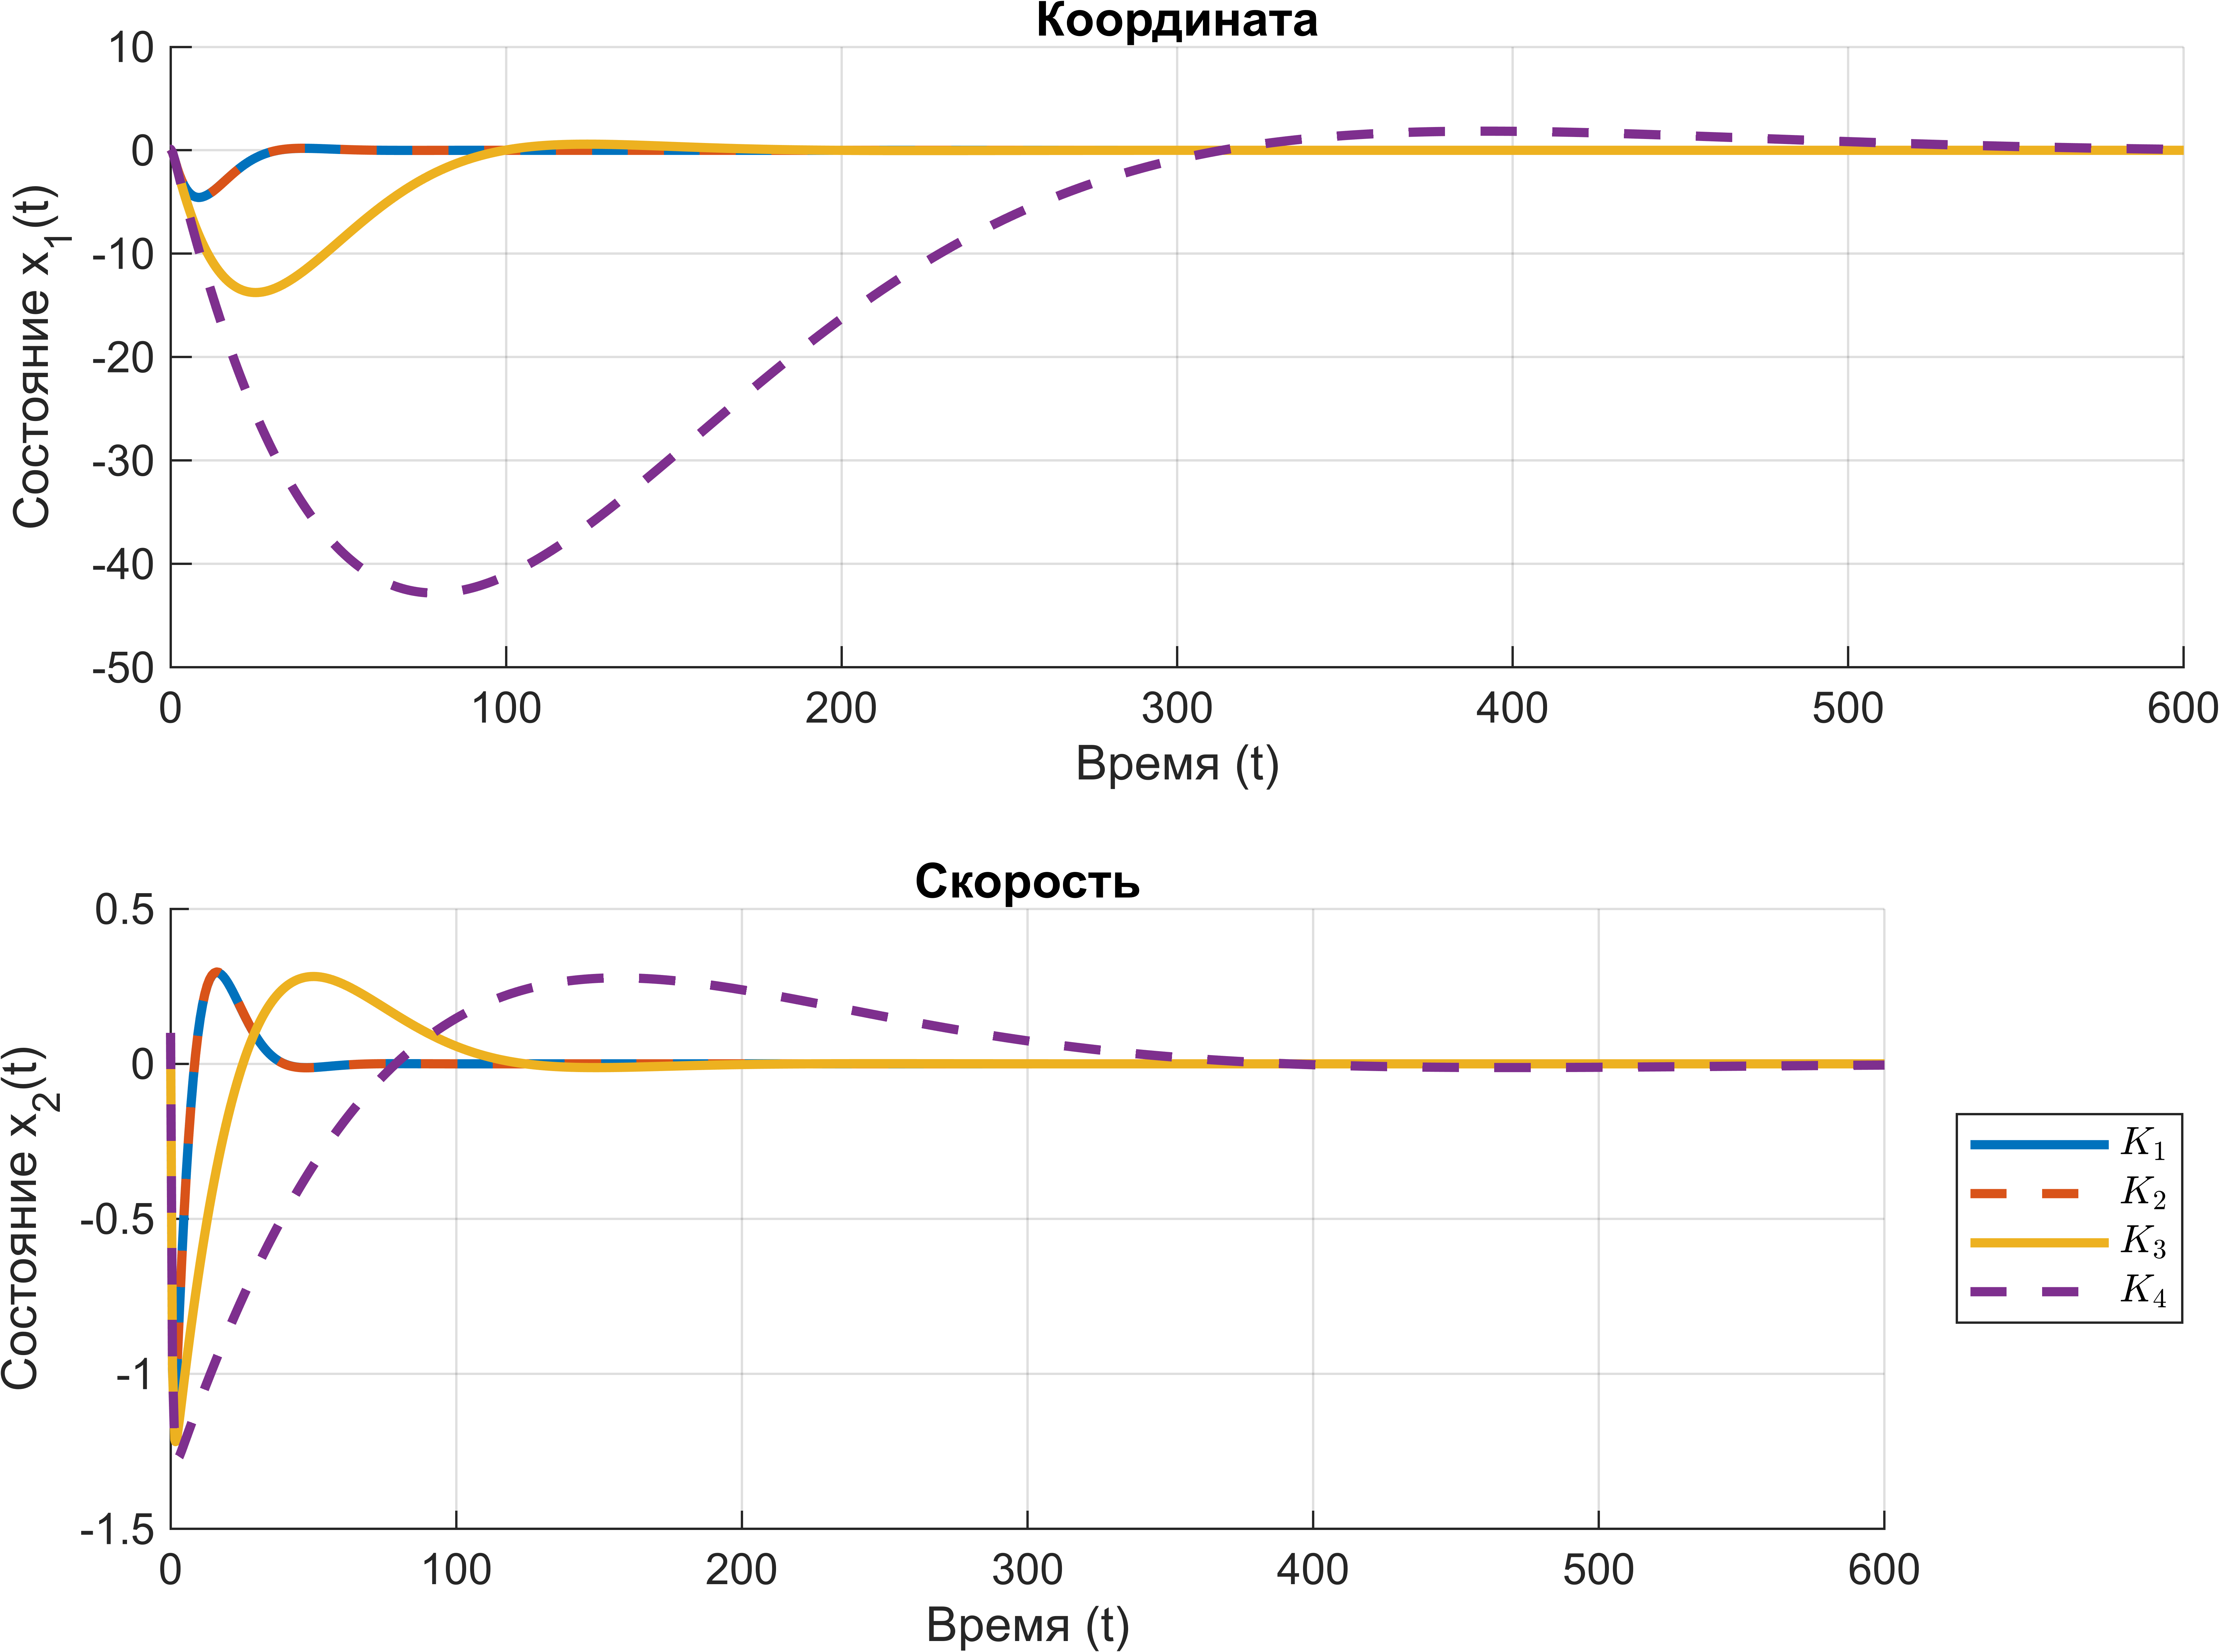
\includegraphics[width=0.8\linewidth]{figs/6.2.sim.x.png}
    \caption{Состояние тележки при различных весовых 
    матрицах LQR-регулятора}
    \label{fig:6.2.sim.x}
\end{figure}

\begin{figure}[H]
    \centering
    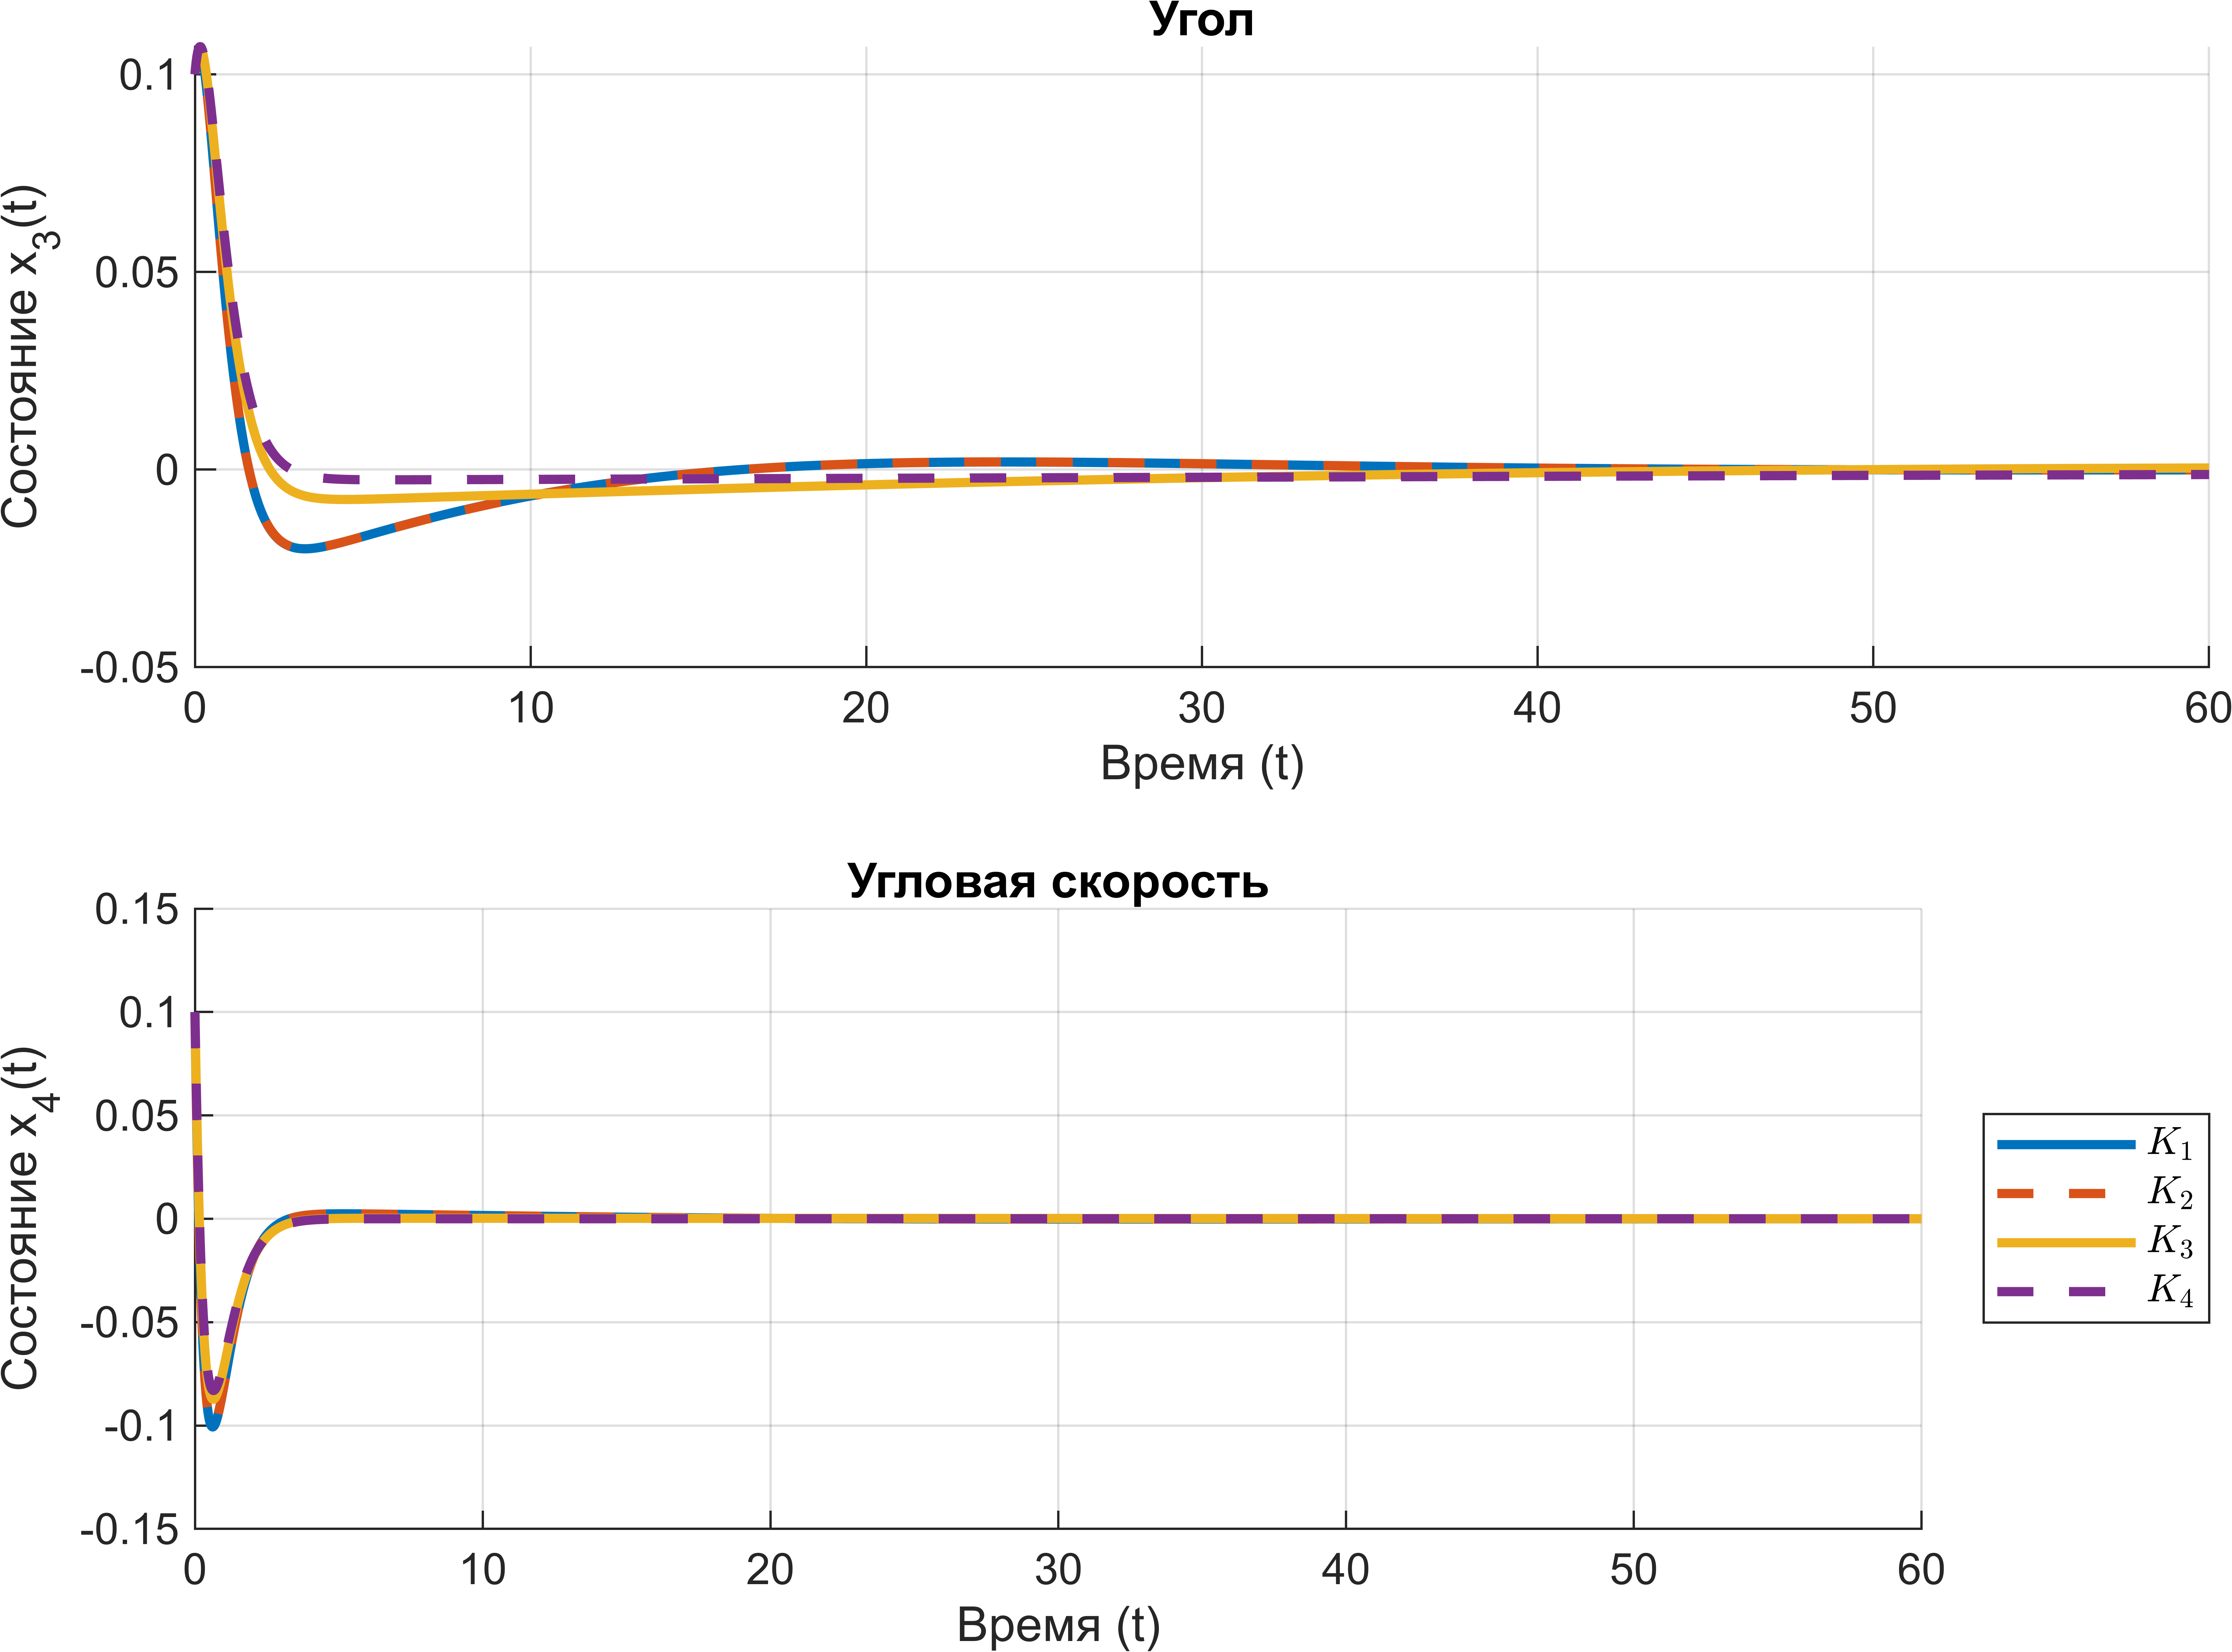
\includegraphics[width=0.8\linewidth]{figs/6.2.sim.phi.png}
    \caption{Состояние маятника при различных весовых матрицах LQR-регулятора}
    \label{fig:6.2.sim.phi}
\end{figure}

\begin{figure}[H]
    \centering
    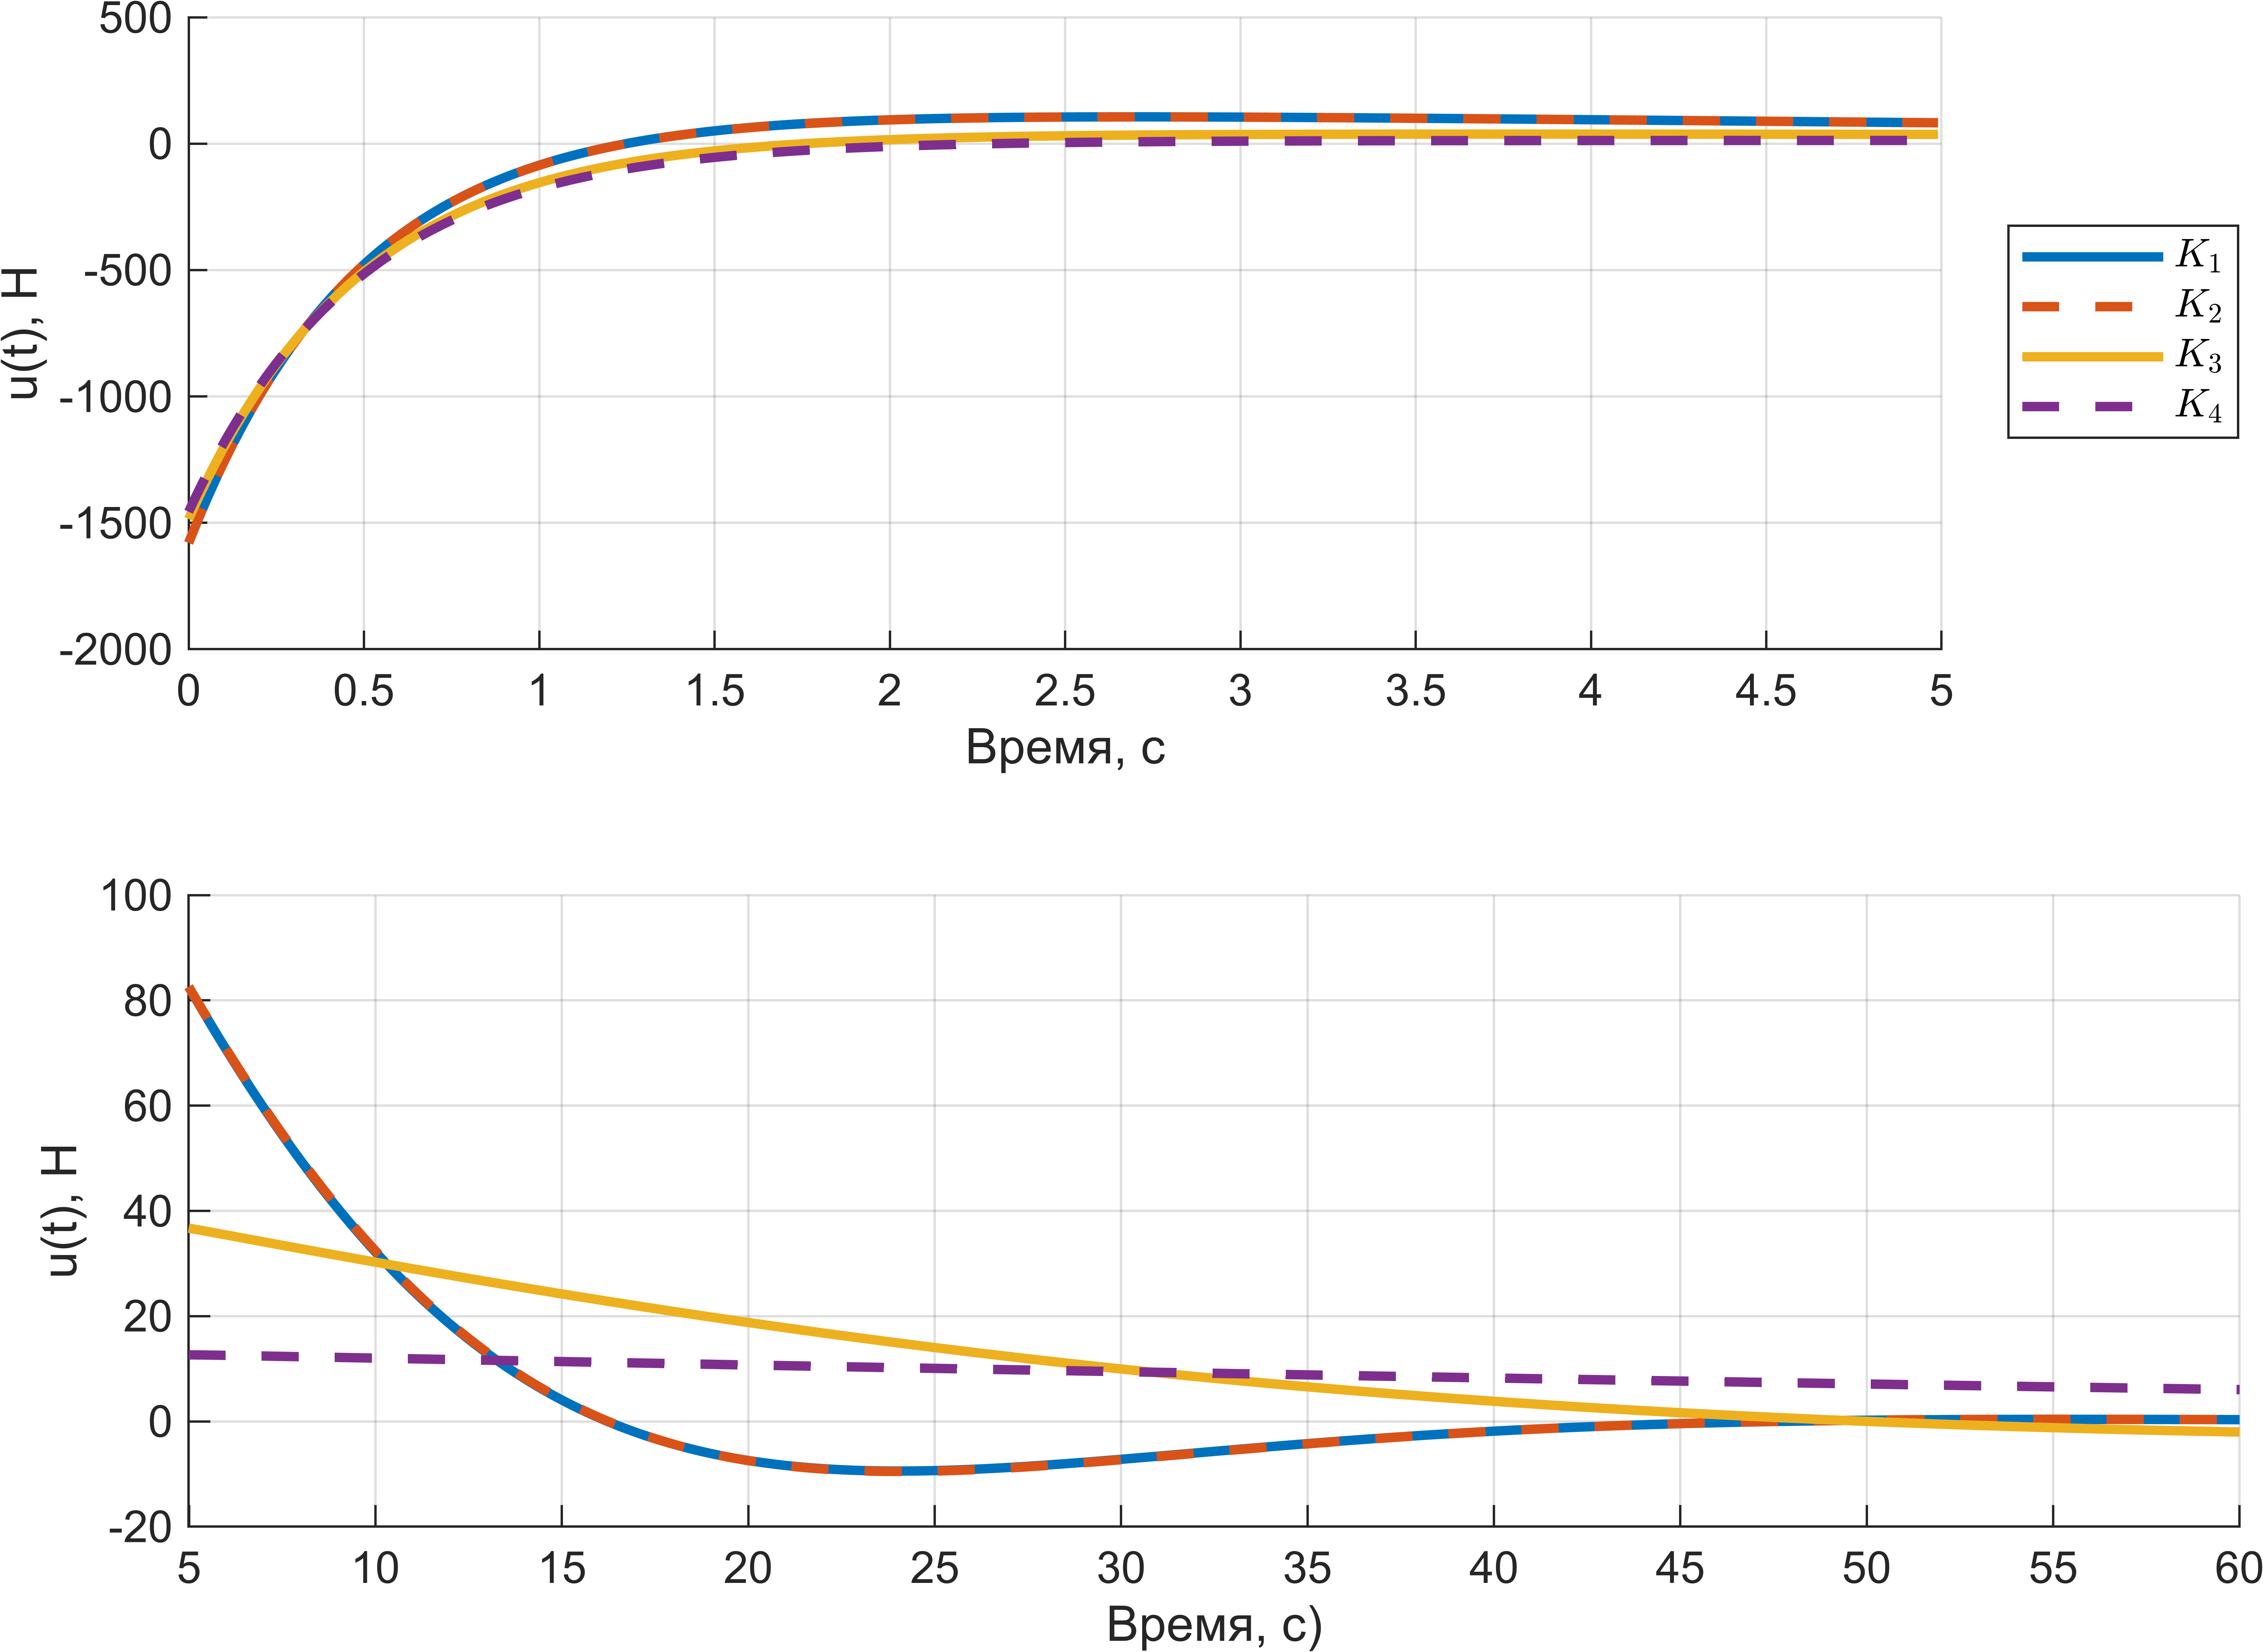
\includegraphics[width=0.8\linewidth]{figs/6.2.sim.u.png}
    \caption{Управление при различных весовых матрицах LQR-регулятора}
    \label{fig:6.2.sim.u}
\end{figure}

\noindent Регуляторы выполняют свою задачу: $Q_1$ приводит состояние к 0
быстрее всех, $Q_2$ очень похож на $Q_1$, но координата тележки при нем 
сходится быстрее всего, при $Q_3$ сходится быстрее всего отклонение маятника,
$Q_4$ - самый "слабый" регулятор, при нем прилагается мимнимальное управление, что
отлично видно на \autoref{fig:6.2.sim.u}. 

\begin{table}[H]
    \centering
    \caption{\label{tab:6.2}Влияние весов на характеристики системы}
    \begin{tabular}{|c|c|c|c|}
        \hline
        $Q$ & Макс. упр., H & Макс. откл. тележки, м & Макс. угол маятника, $^\circ$ \\
        \hline
        1 & 1579.6   & 4.6  & 6.31   \\
        2    & 1578.9   & 4.6  & 6.31   \\
        3    & 1485.0  & 14.0  & 6.31  \\
        4    & 1456.3  & 43.0  & 6.31  \\
        \hline
    \end{tabular}
\end{table}

\noindent Максимальное отклонение маятника от вертикали,
максимальное горизонтальное смещение тележки и 
максимальное значение управляющего сигнала при каждом наборе весов
можно увидеть в \autoref{tab:6.2}. Отклонение маятника лишь слегка
было превышено, относительно начального (5.73$^\circ$), в самом начале
симуляций. Как можно было и ожидать, при $Q_4$ наименьшее максимальное
управление, при нем же и наибольшее отклонение координаты тележки, что
говорит о том, что в каждом моменте была приложена минимальная сила,
это и видно по графику управления \ref{fig:6.2.sim.u}.

\section{Синтез фильтра Калмана}

Синтезируем фильтр Калмана в непрерывном времени на основе линейной 
модели \eqref{eq:sys} и применим его для оценки вектора 
состояния нелинейной системы \eqref{eq:origsys}. 
Выберем регулятор $K_1$ из предыдущего
пункта, на котором проверим работоспособность фильтра.
Выберем две матрицы $Q$; $R$ зафиксируем на 1, потому что в фильтре Калмана
или LQE важно именно отношение чисел весовых матриц. Пусть
\begin{equation*}
    Q_1=\begin{bmatrix}
        100 & 0 & 0 & 0 \\
        0 & 100 & 0 & 0 \\
        0 & 0 & 100 & 0 \\
        0 & 0 & 0 & 100
    \end{bmatrix},\quad
    Q_2=\begin{bmatrix}
        0.01 & 0 & 0 & 0 \\
        0 & 0.01 & 0 & 0 \\
        0 & 0 & 0.01 & 0 \\
        0 & 0 & 0 & 0.01
    \end{bmatrix},
\end{equation*}
в первом случае мы говорим, что в состоянии мало шумов, во втором, что в
выходе мало шумов. Решением уравения Риккати:
\begin{equation*}
    AP+PA^T+Q-PC^TR^{-1}CP=0,\quad L=-PC^TR^{-1}
\end{equation*}
с помощью icare, получим
\begin{gather*}
        L_1=\begin{bmatrix}
-10.95 & -0.007686\\
-10.0 & -0.1468\\
-0.007686 & -11.41\\
-0.02512 & -15.12
    \end{bmatrix},\quad
    \sigma(A+L_2C)=\left\{ 
\begin{array}{c}
-9.9493\\
-10.364\\
-1.0051\\
-1.0487
\end{array}
     \right\}\\
             L_2=\begin{bmatrix}
-0.4605 & -0.09494\\
-0.1056 & -0.2394\\
-0.09494 & -4.126\\
-0.196 & -8.51
    \end{bmatrix},\quad
    \sigma(A+L_2C)=\left\{ 
\begin{array}{c}
-0.22918\pm0.21799\,\mathrm{i}\\
-2.0201\\
-2.1077
\end{array}
     \right\}.
\end{gather*}
Начальным состоянием объекта возьмем 0.1, а наблюдателя - 0.
Графики состояния наблюдателя в сравнении с реальным состоянием можно
увидеть на \autoref{fig:6.3.sim}, а ошибку оценки --- на \autoref{fig:6.3.sim.err}.
Как видно, при большой уверенности в состоянии (уверенности отсутствия шумов в нем) 
- $Q_1$ фильтр быстрее сходится. При уверенности в наличии шумов в состоянии 
- $Q_2$ фильтр сходится медленнее. В обоих случаях фильтр Калмана 
корректно оценивает состояния системы.
\begin{figure}[H]
    \centering
    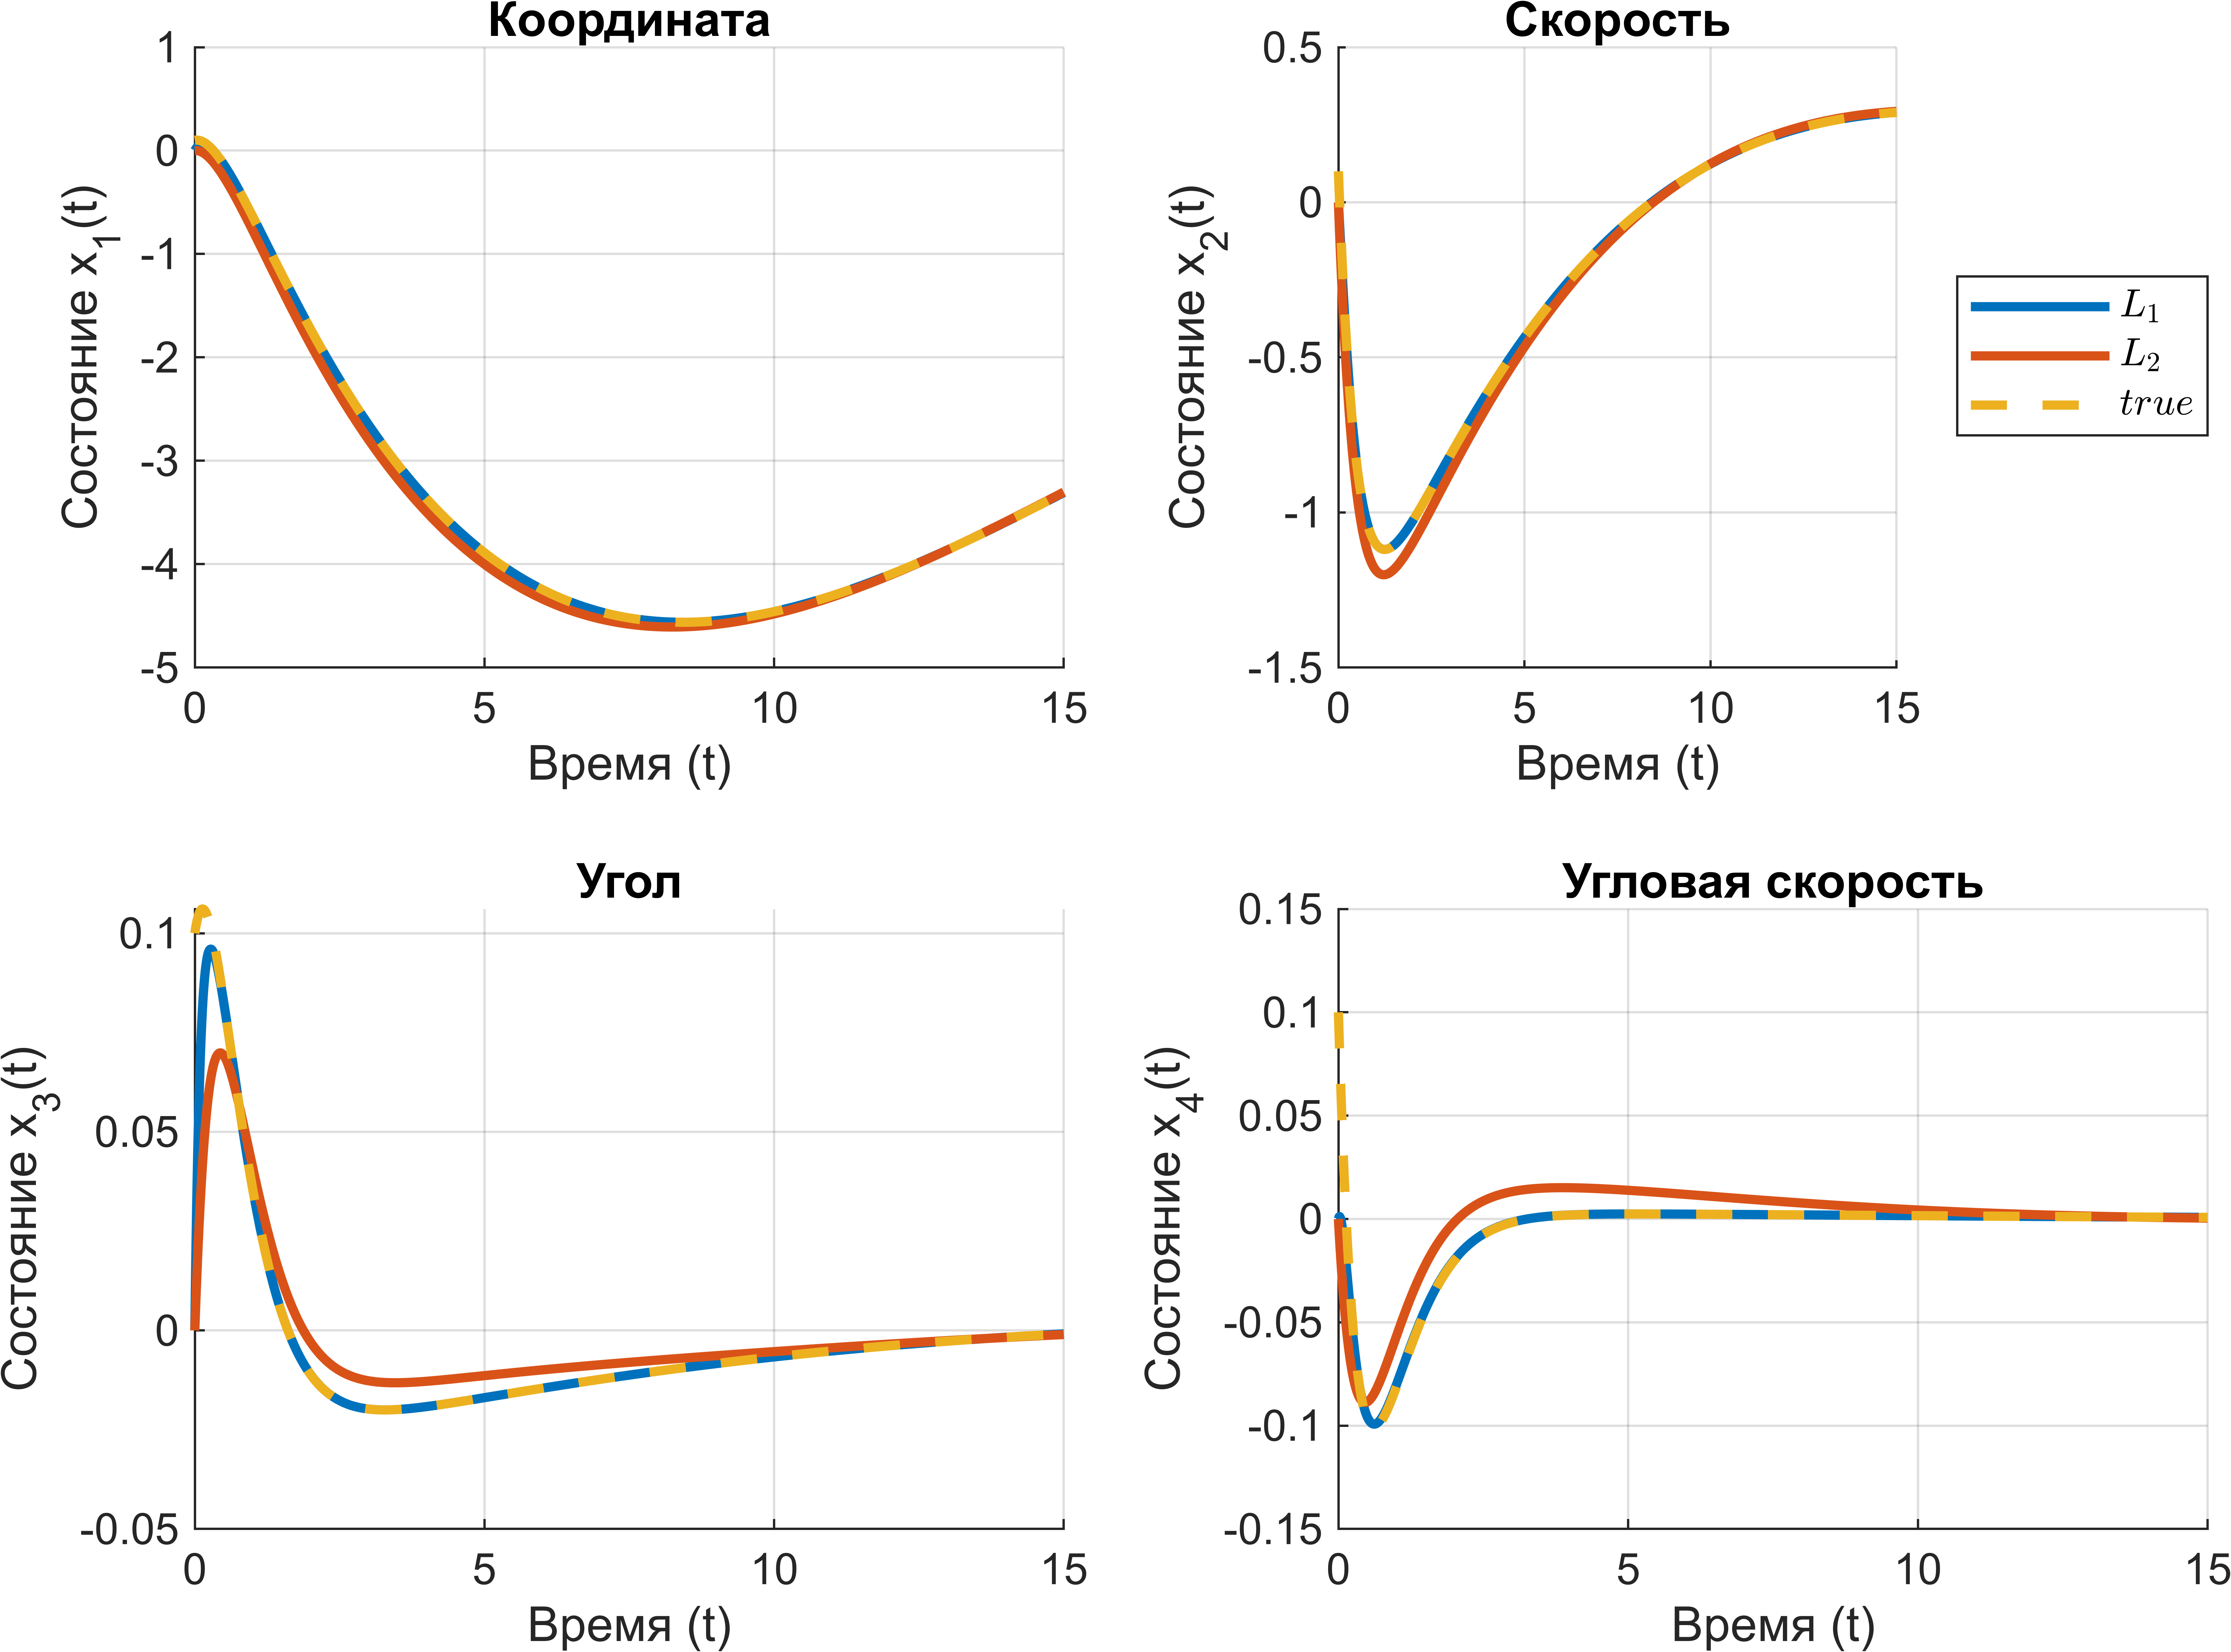
\includegraphics[width=0.9\linewidth]{figs/6.3.sim.png}
    \caption{Моделирование работы фильтра Калмана при различных 
    весовых матрицах}
    \label{fig:6.3.sim}
\end{figure}
\begin{figure}[H]
    \centering
    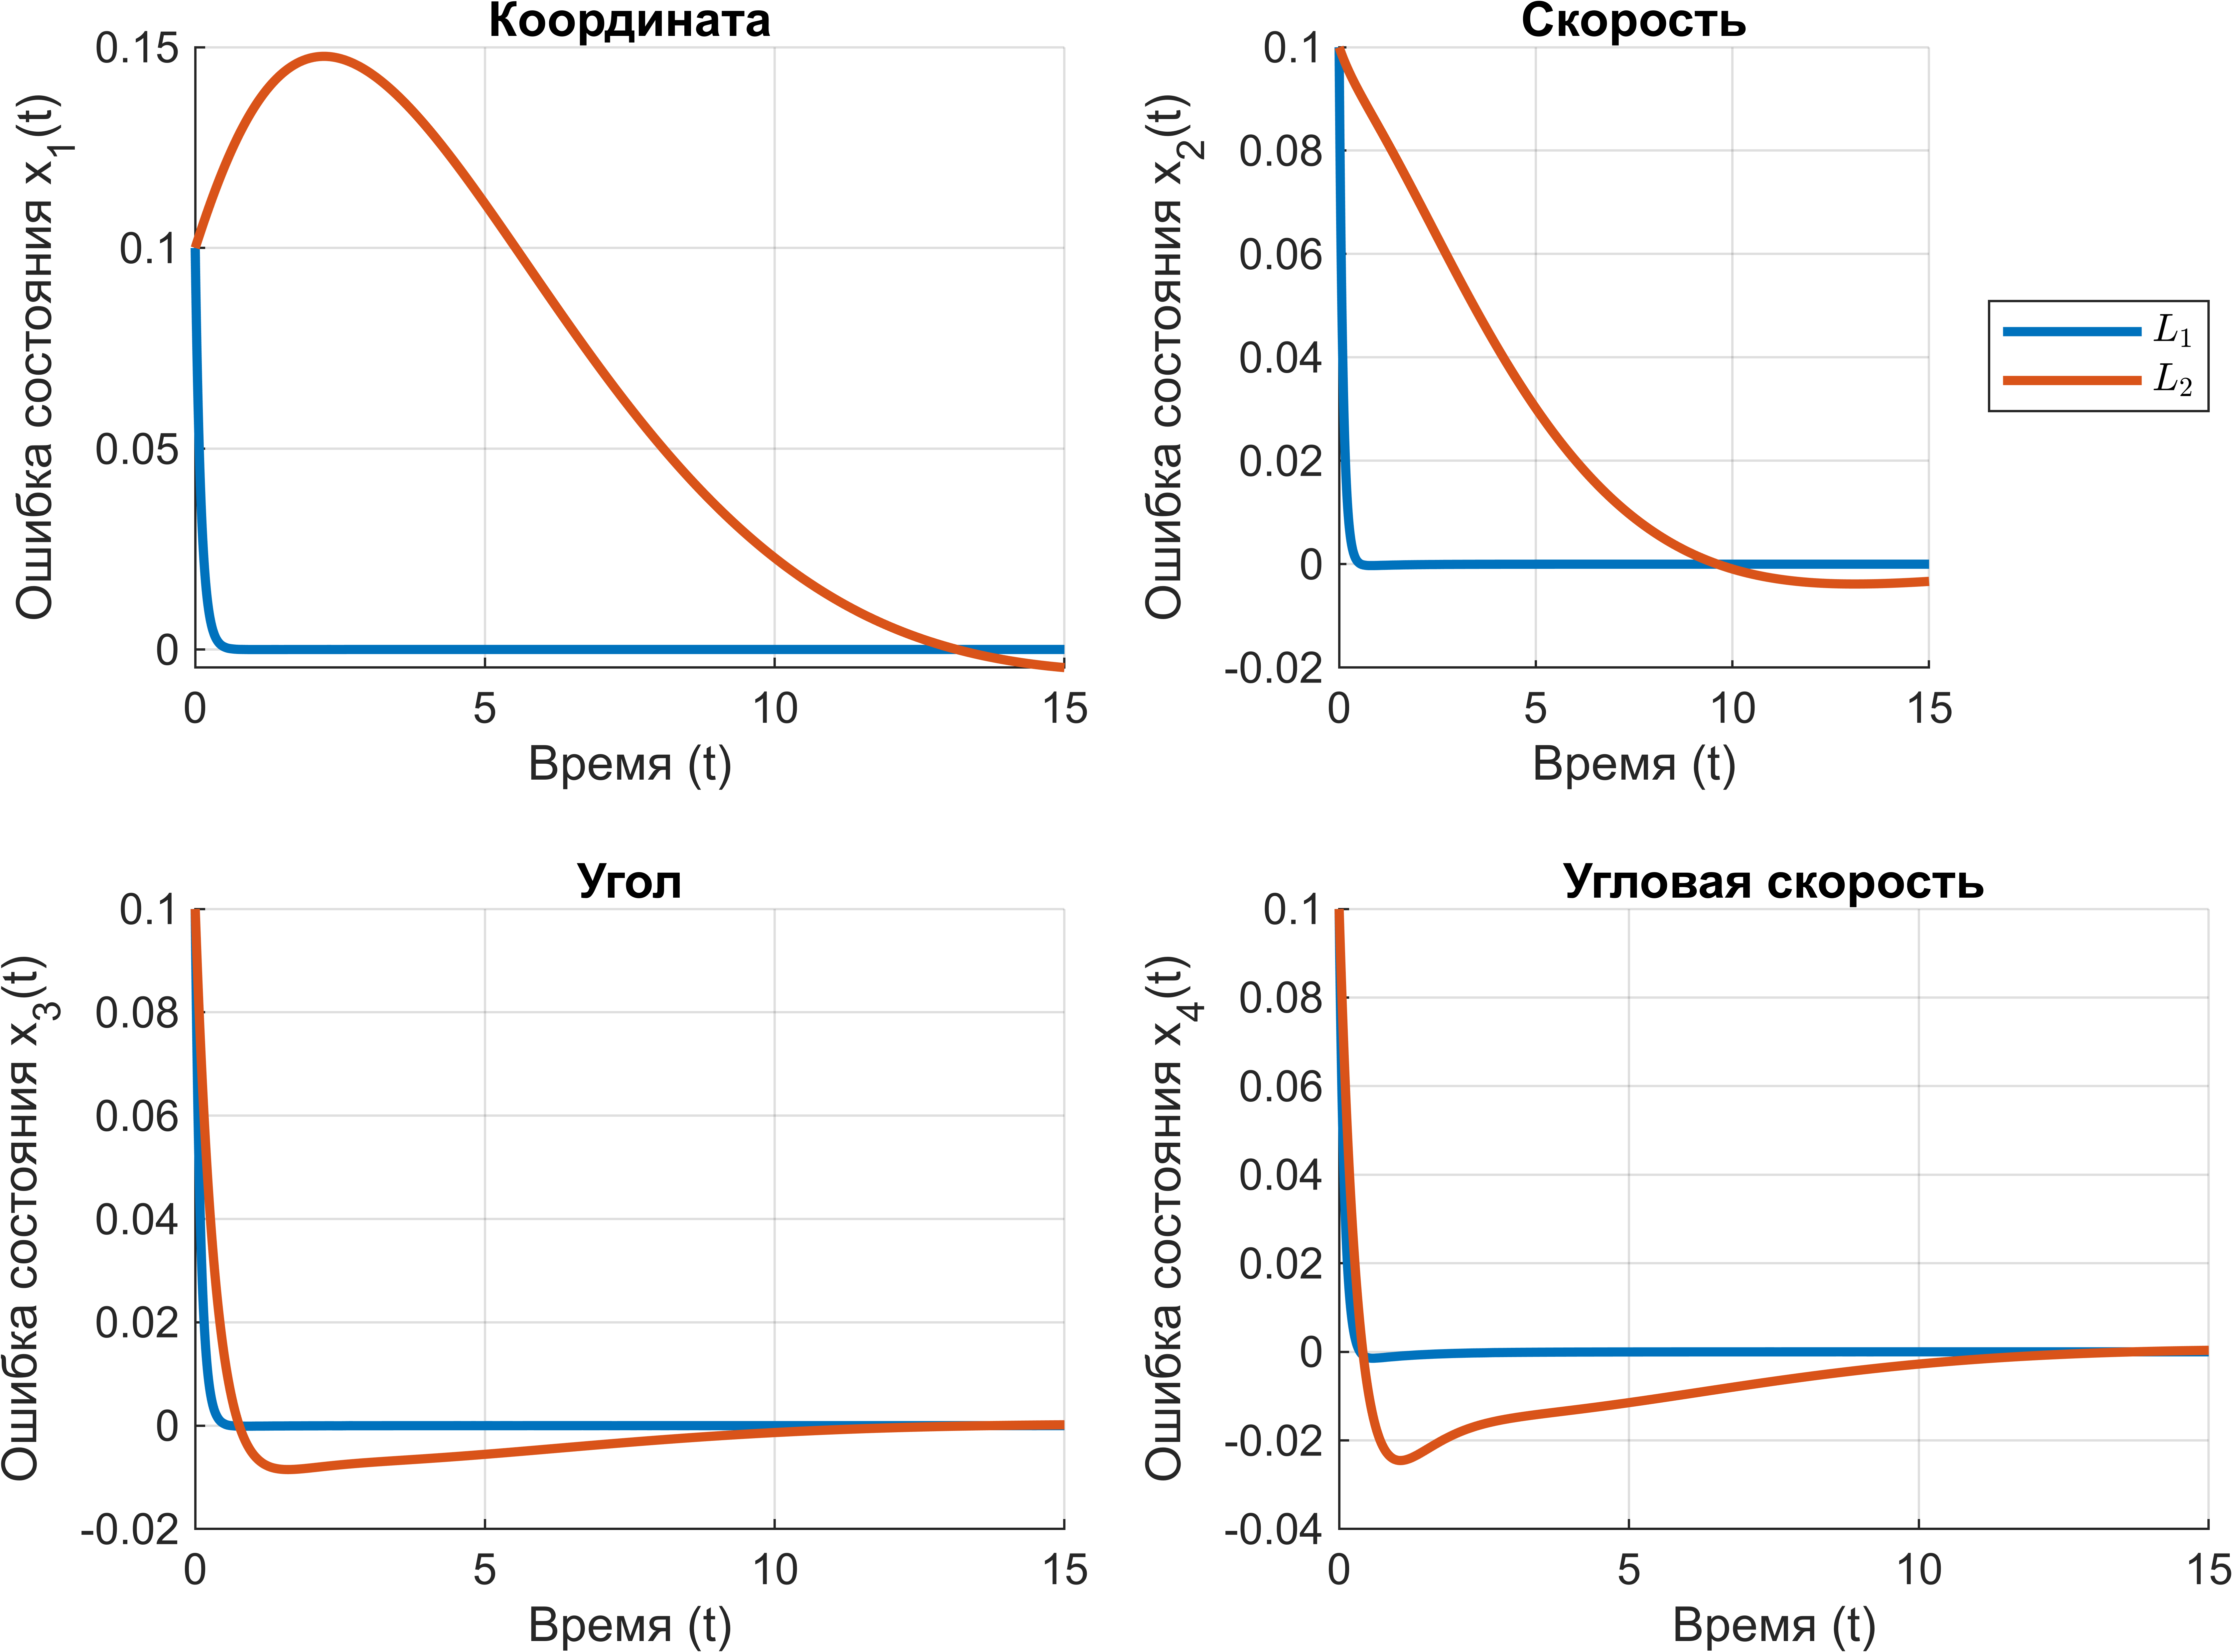
\includegraphics[width=0.9\linewidth]{figs/6.3.sim.err.png}
    \caption{Ошибка фильтра Калмана при различных весовых матрицах}
    \label{fig:6.3.sim.err}
\end{figure}

\section{LQG для линейной модели}

Применим LQR-регулятор совместно с фильтром Калмана для управления 
линейной моделью
\begin{equation}
    \label{eq:sys.noise}
    \begin{cases}
        \dot x=Ax+Bu+Df,\\
        y=Cx+\xi,
    \end{cases}
\end{equation}
в которой сигналы $f$ и $\xi$ заданы как белый гауссовский шум
с матрицами ковариации $0.1$ и $\begin{bmatrix}
    0.01&0\\0&0.01
\end{bmatrix}$ соответственно. Возмущения в выходе меньше, чем в состоянии.
Воспользуемся теми же матрицами регулятора и наблюдателей как в прошлом 
пункте, но вид регулятора теперь \eqref{eq:3.3.estred}. Результат
увидеть на \autoref{fig:6.4.sim.1}, ошибку фильтра Калмана — на 
\autoref{fig:6.4.sim.1.err}. Аналогично, для наблюдателя $L_2$ — 
на \autoref{fig:6.4.sim.2} и ошибку на \autoref{fig:6.4.sim.2.err}. 
Как видно, LQG успешно удерживает маятник в верхнем положении, была
достигнута статичность в ошибке наблюдателя. При $L_1$, который синтезировался
с уверенностью в отстутвии шума в состоянии, имеется довольно большая 
ошибка наблюдателя:
\begin{itemize}
    \item максимальная ошибка оценки координаты тележки~--- 80 см,
    \item максимальная ошибка оценки скорости тележки~--- 8 cм/с,
    \item максимальная ошибка оценки угла маятника~--- 5.16$^\circ$,
    \item максимальная ошибка оценки угловой скорости маятника~--- 8.60$^\circ$/с.
\end{itemize}
При $L_2$, который синтезировался
с уверенностью в наличии шума в состоянии и малом шуме в выходе (что соответсвует реальности), 
ошибка гораздо меньше:
\begin{itemize}
    \item максимальная ошибка оценки координаты тележки~--- 1 см,
    \item максимальная ошибка оценки скорости тележки~--- 1 cм/с,
    \item максимальная ошибка оценки угла маятника~--- 3.44$^\circ$,
    \item максимальная ошибка оценки угловой скорости маятника~--- 8.03$^\circ$/с.
\end{itemize}
Ожидаемо, стабилизировать систему не получилось, но это и не является целью LQG.

\begin{figure}[H]
    \centering
    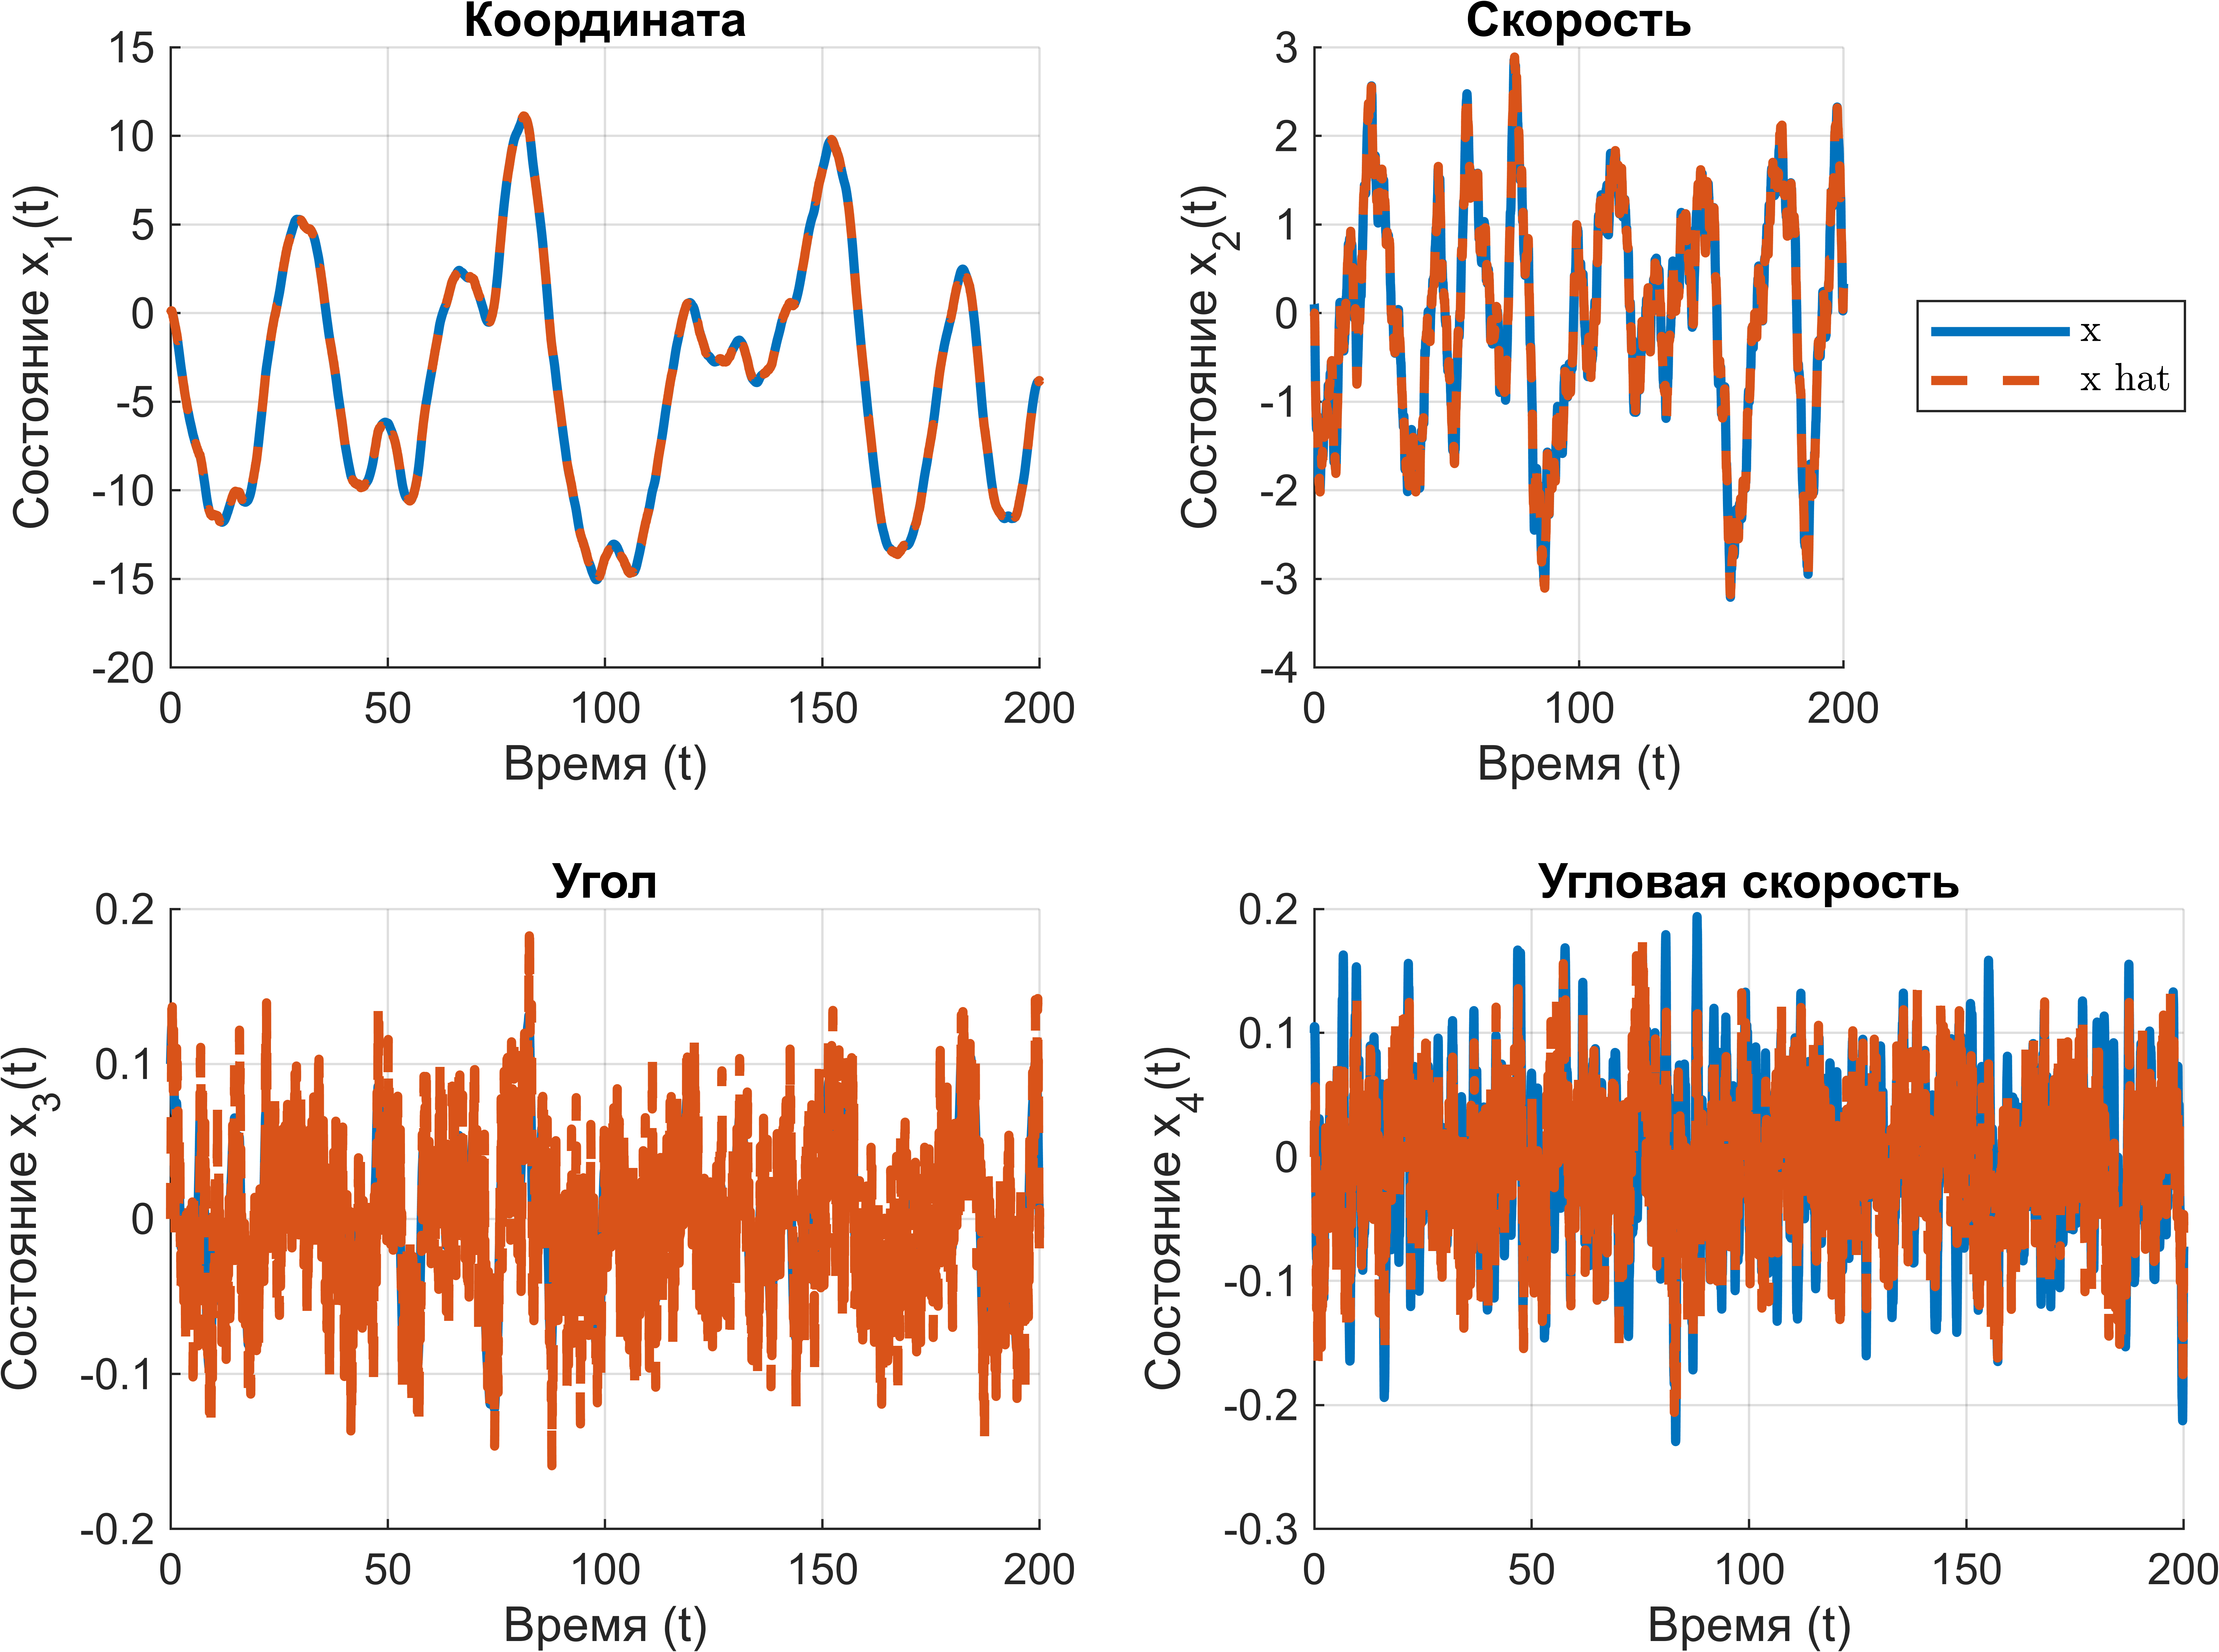
\includegraphics[width=0.9\linewidth]{figs/6.4.sim.1.png}
    \caption{Моделирование работы LQG при $L_1$}
    \label{fig:6.4.sim.1}
\end{figure}
\begin{figure}[H]
    \centering
    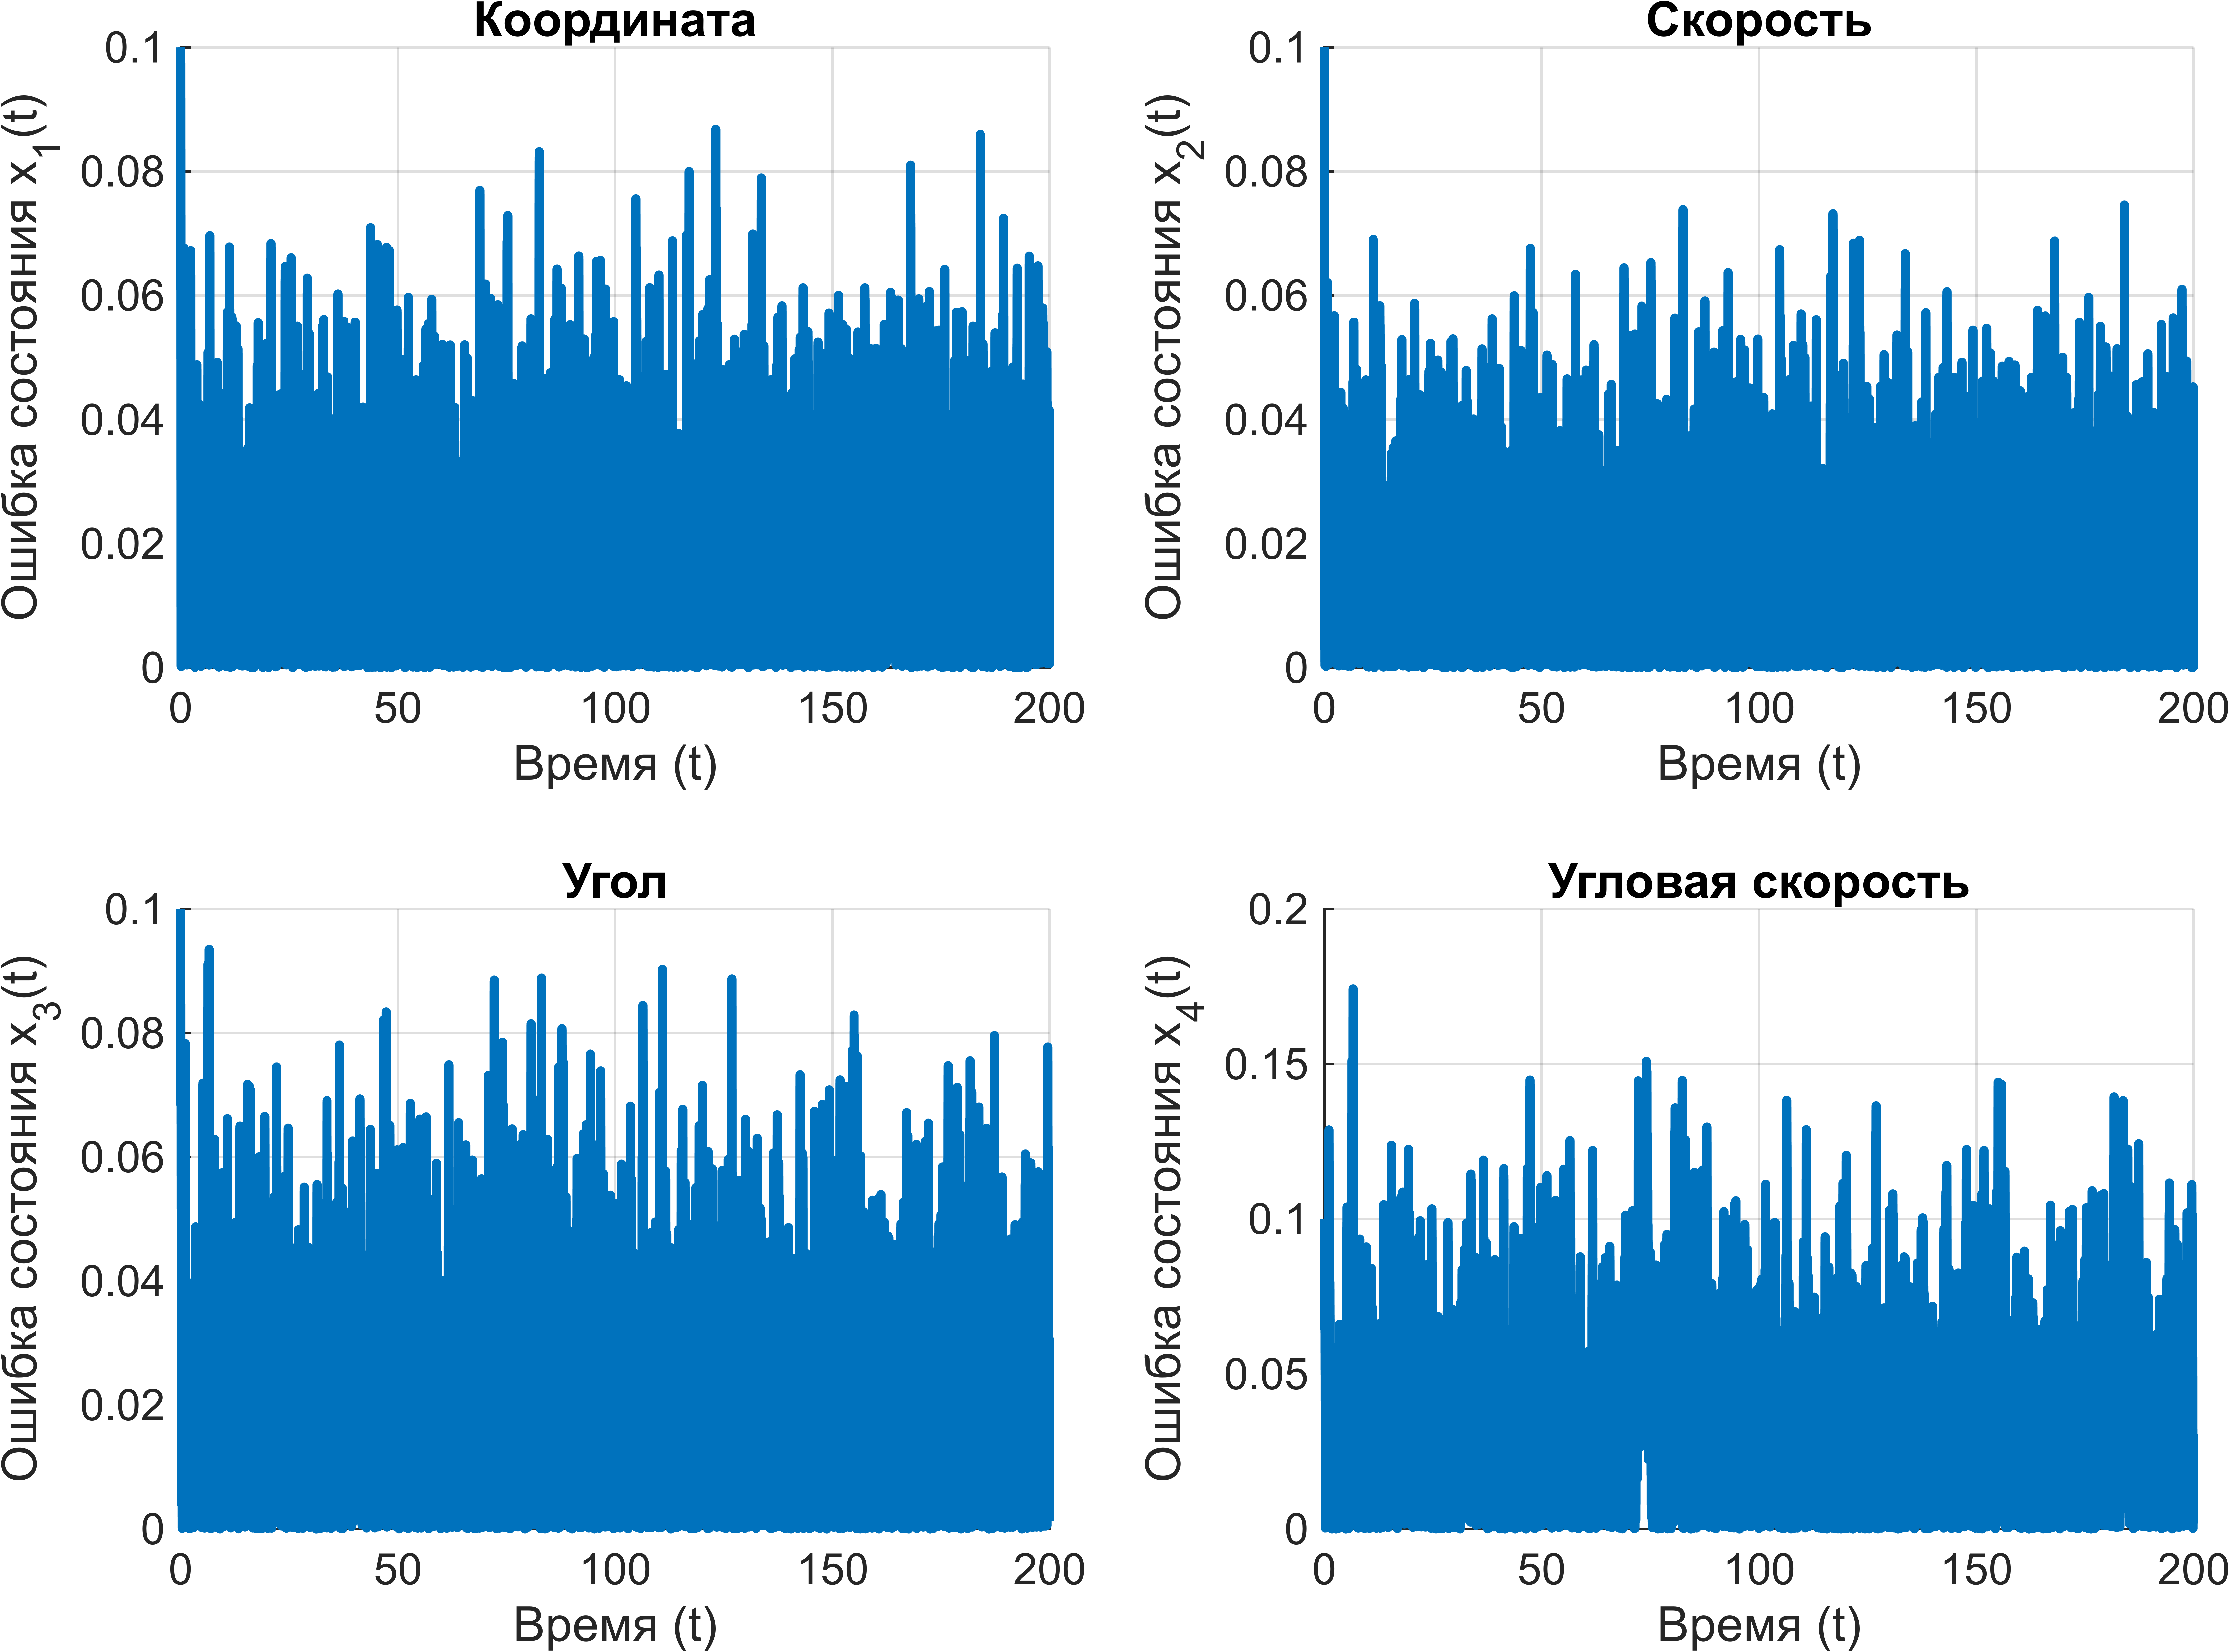
\includegraphics[width=0.9\linewidth]{figs/6.4.sim.1.err.png}
    \caption{Ошибка фильтра Калмана при $L_1$}
    \label{fig:6.4.sim.1.err}
\end{figure}
\begin{figure}[H]
    \centering
    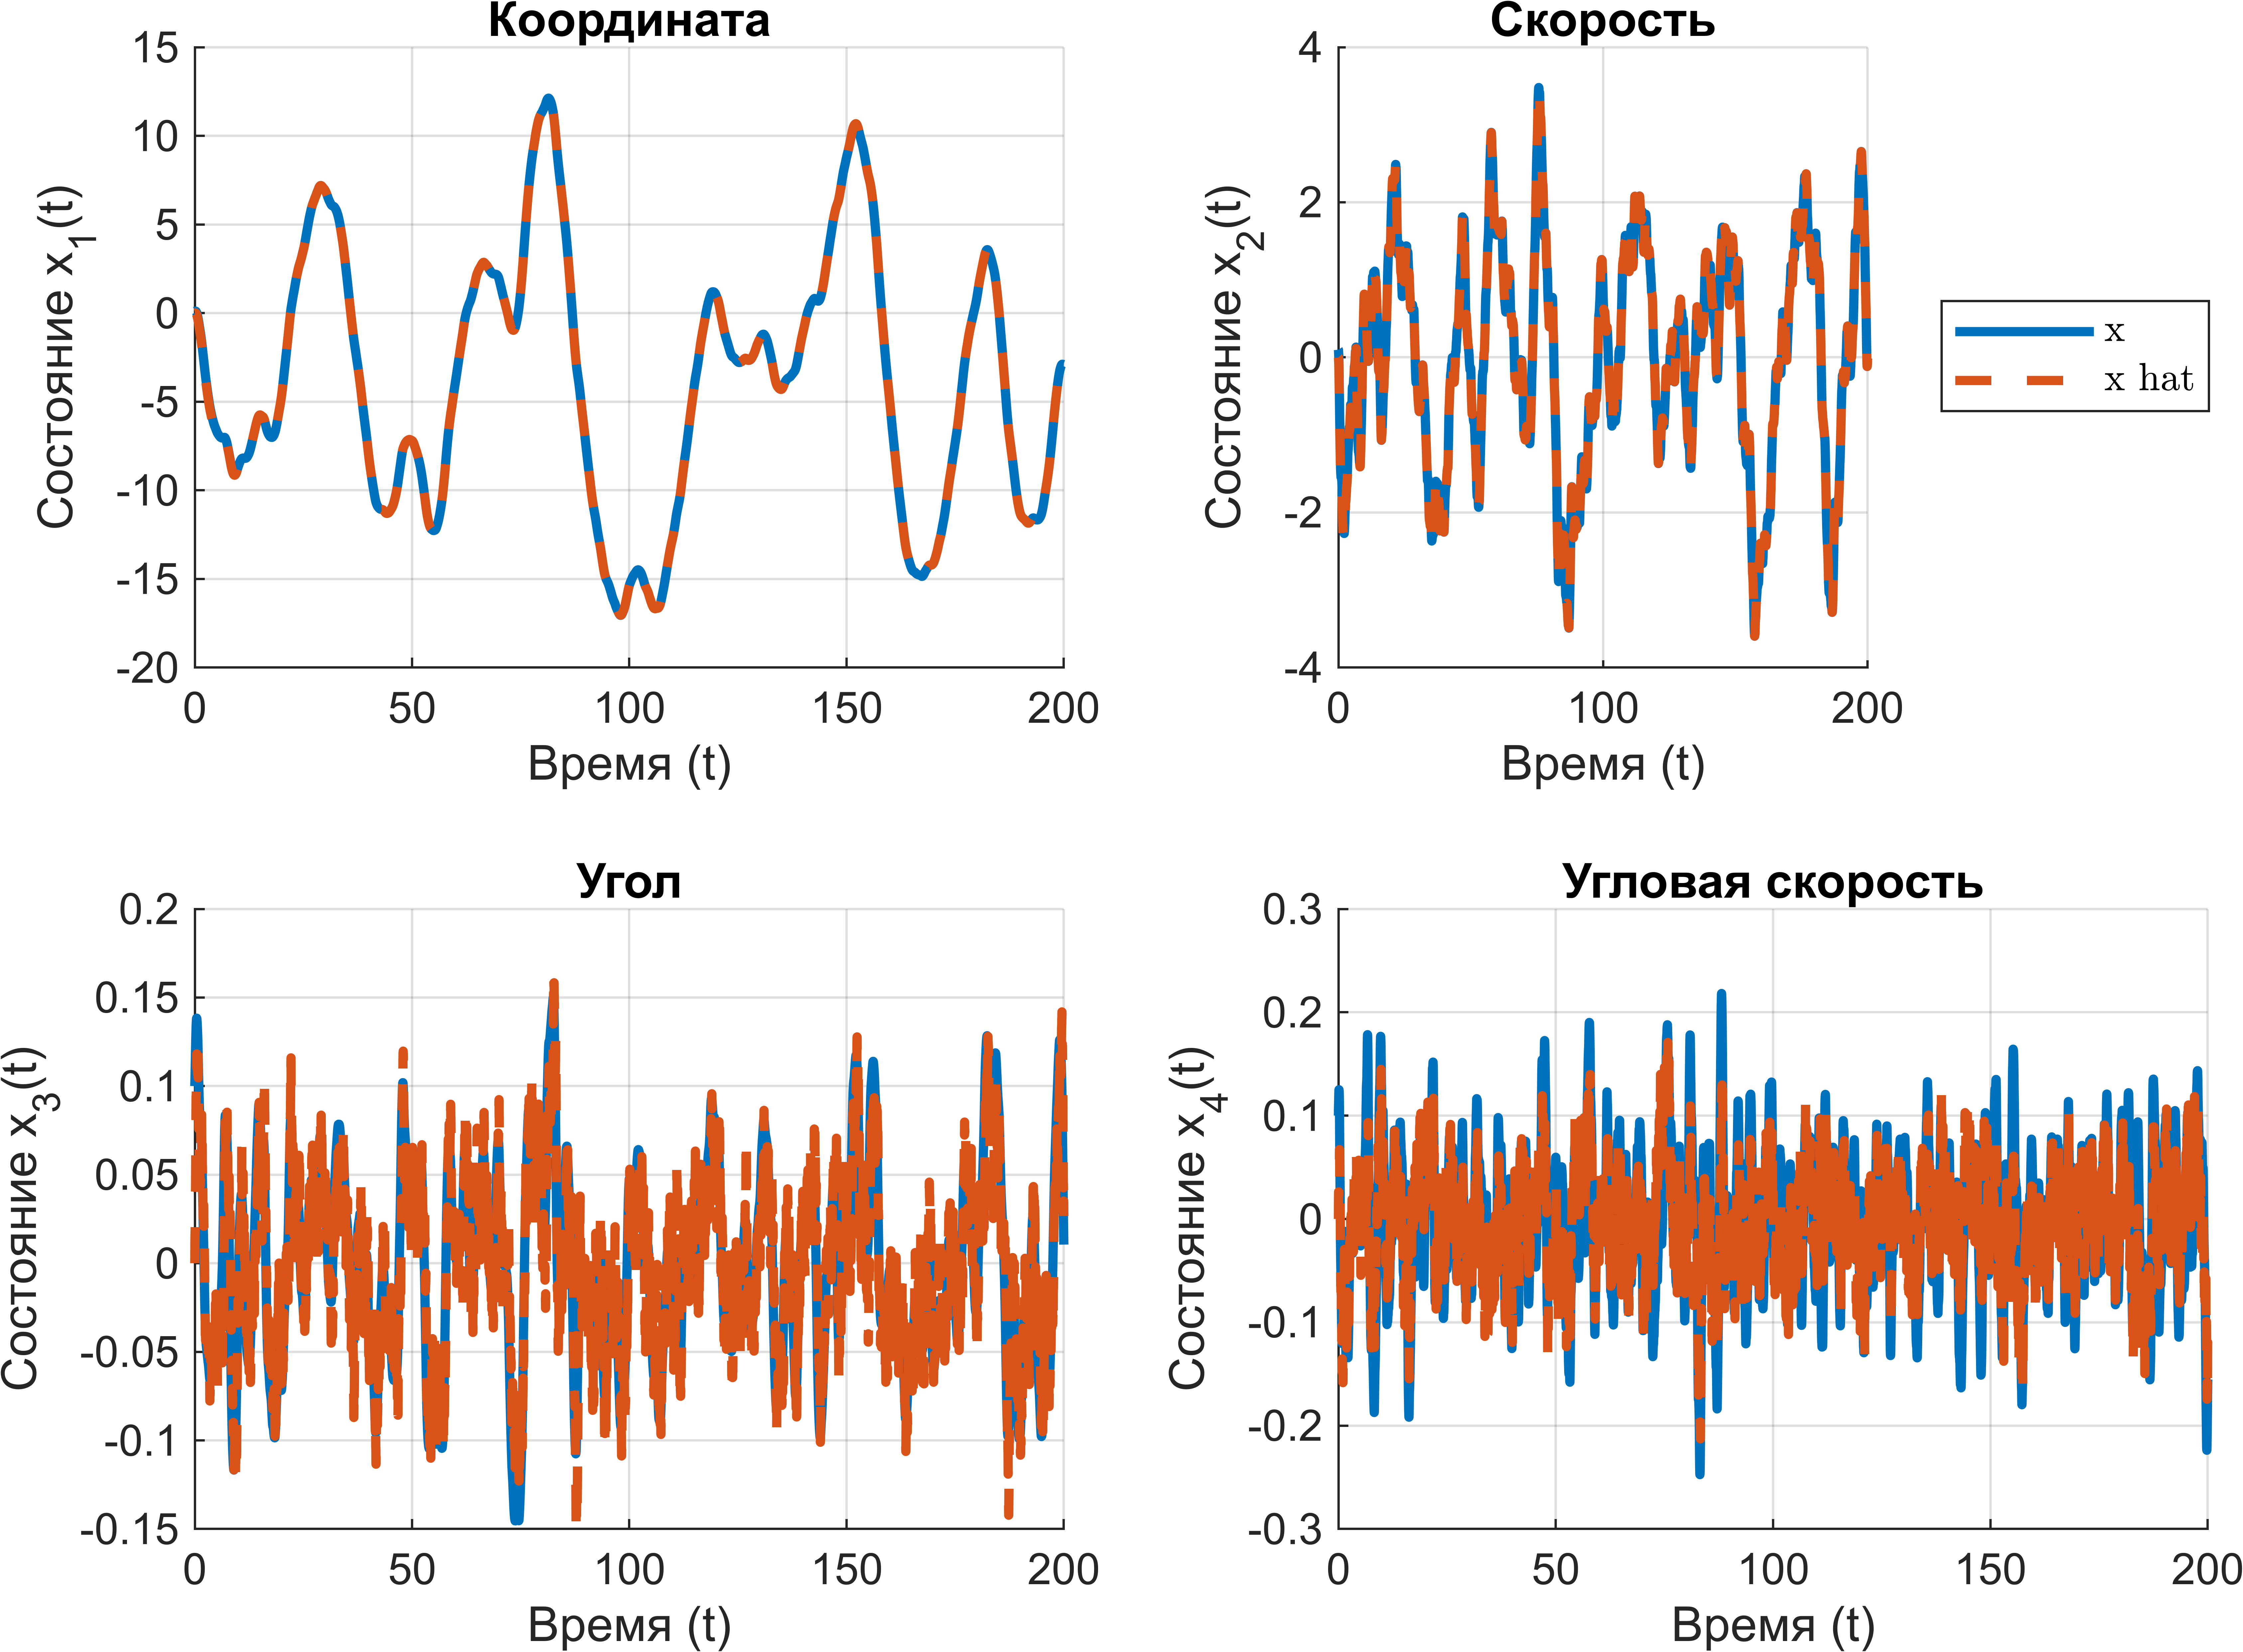
\includegraphics[width=0.9\linewidth]{figs/6.4.sim.2.png}
    \caption{Моделирование работы LQG при $L_2$}
    \label{fig:6.4.sim.2}
\end{figure}
\begin{figure}[H]
    \centering
    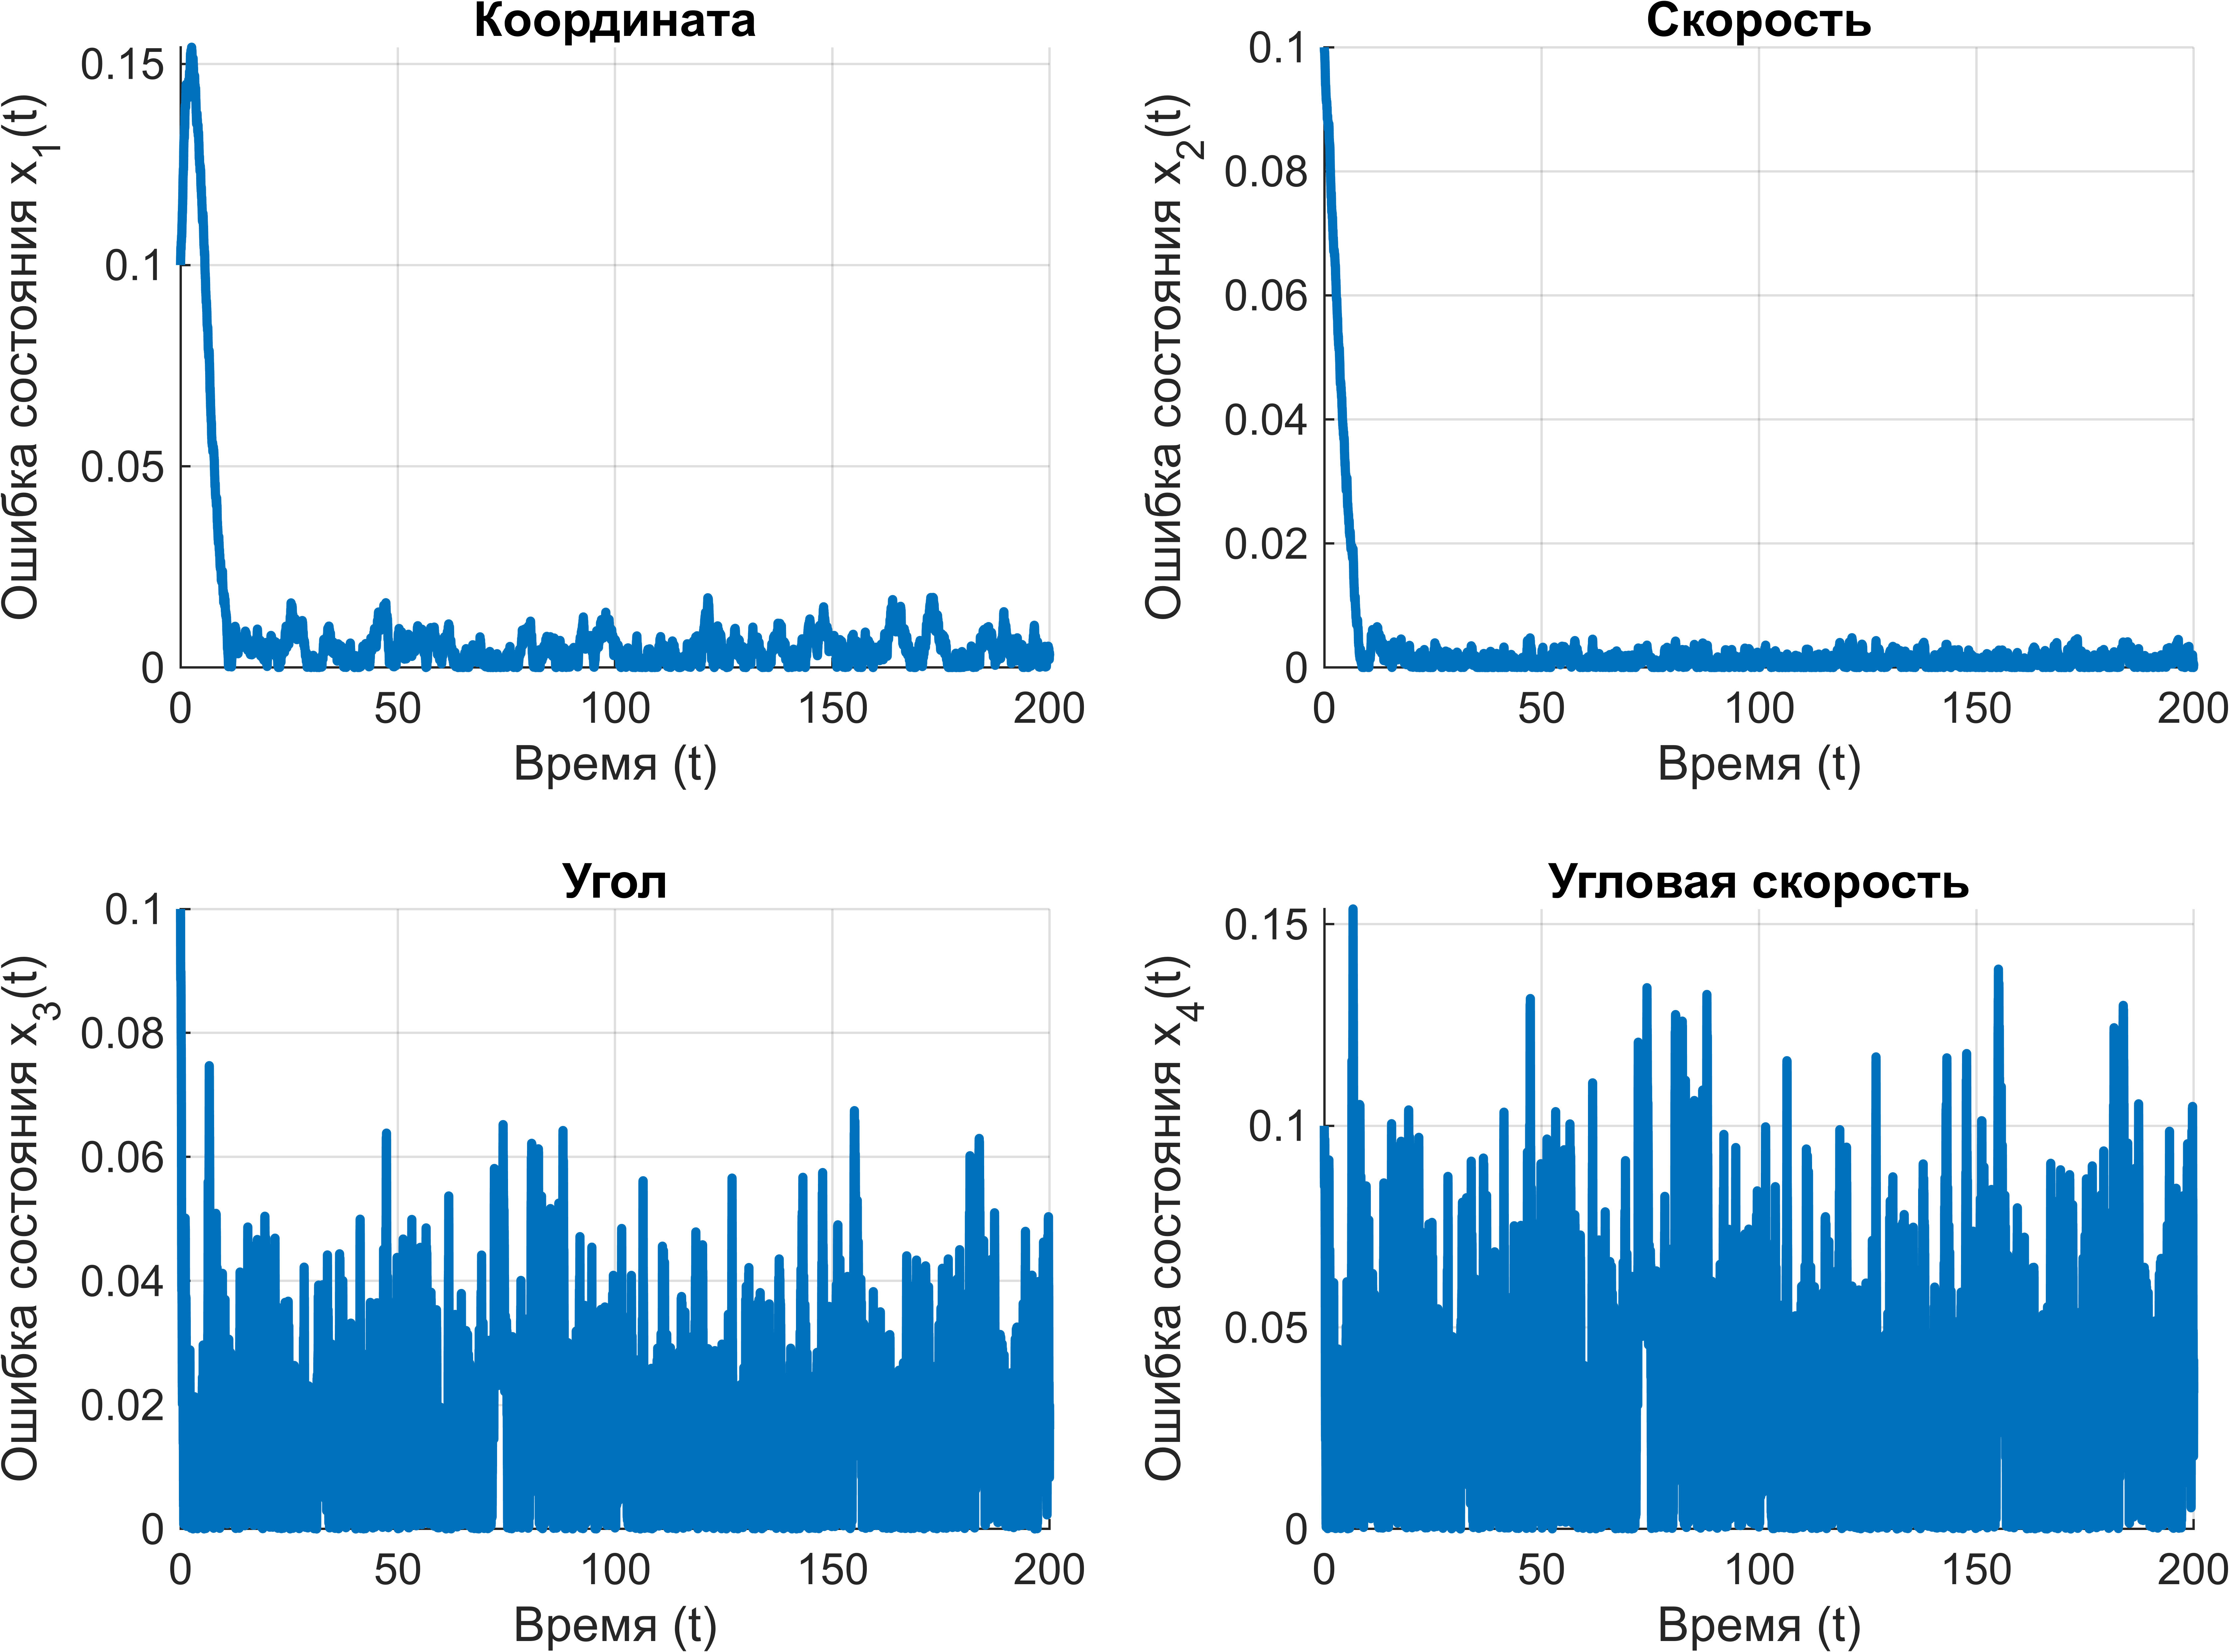
\includegraphics[width=0.9\linewidth]{figs/6.4.sim.2.err.png}
    \caption{Ошибка фильтра Калмана при LQG при $L_2$}
    \label{fig:6.4.sim.2.err}
\end{figure}

\section{LQG для нелинейной модели}

Применим LQR-регулятор совместно с фильтром Калмана для управления 
нелинейной моделью с добавлением шума $\xi$ в выход.
Cигналы $f$ и $\xi$ исопльщуем из предыдущего пункта,
воспользуемся теми же матрицами регулятора и наблюдателей как в прошлом 
пункте. Результат можно
увидеть на \autoref{fig:6.5.sim.1}, ошибку фильтра Калмана — на 
\autoref{fig:6.5.sim.1.err}. Аналогично, для наблюдателя $L_2$ — 
на \autoref{fig:6.5.sim.2} и ошибку на \autoref{fig:6.5.sim.2.err}. 
Как видно, при $L_1$ LQG не справился с удержанием маятника в верхнем положении,
а вот $L_2$ справился.

\begin{figure}[H]
    \centering
    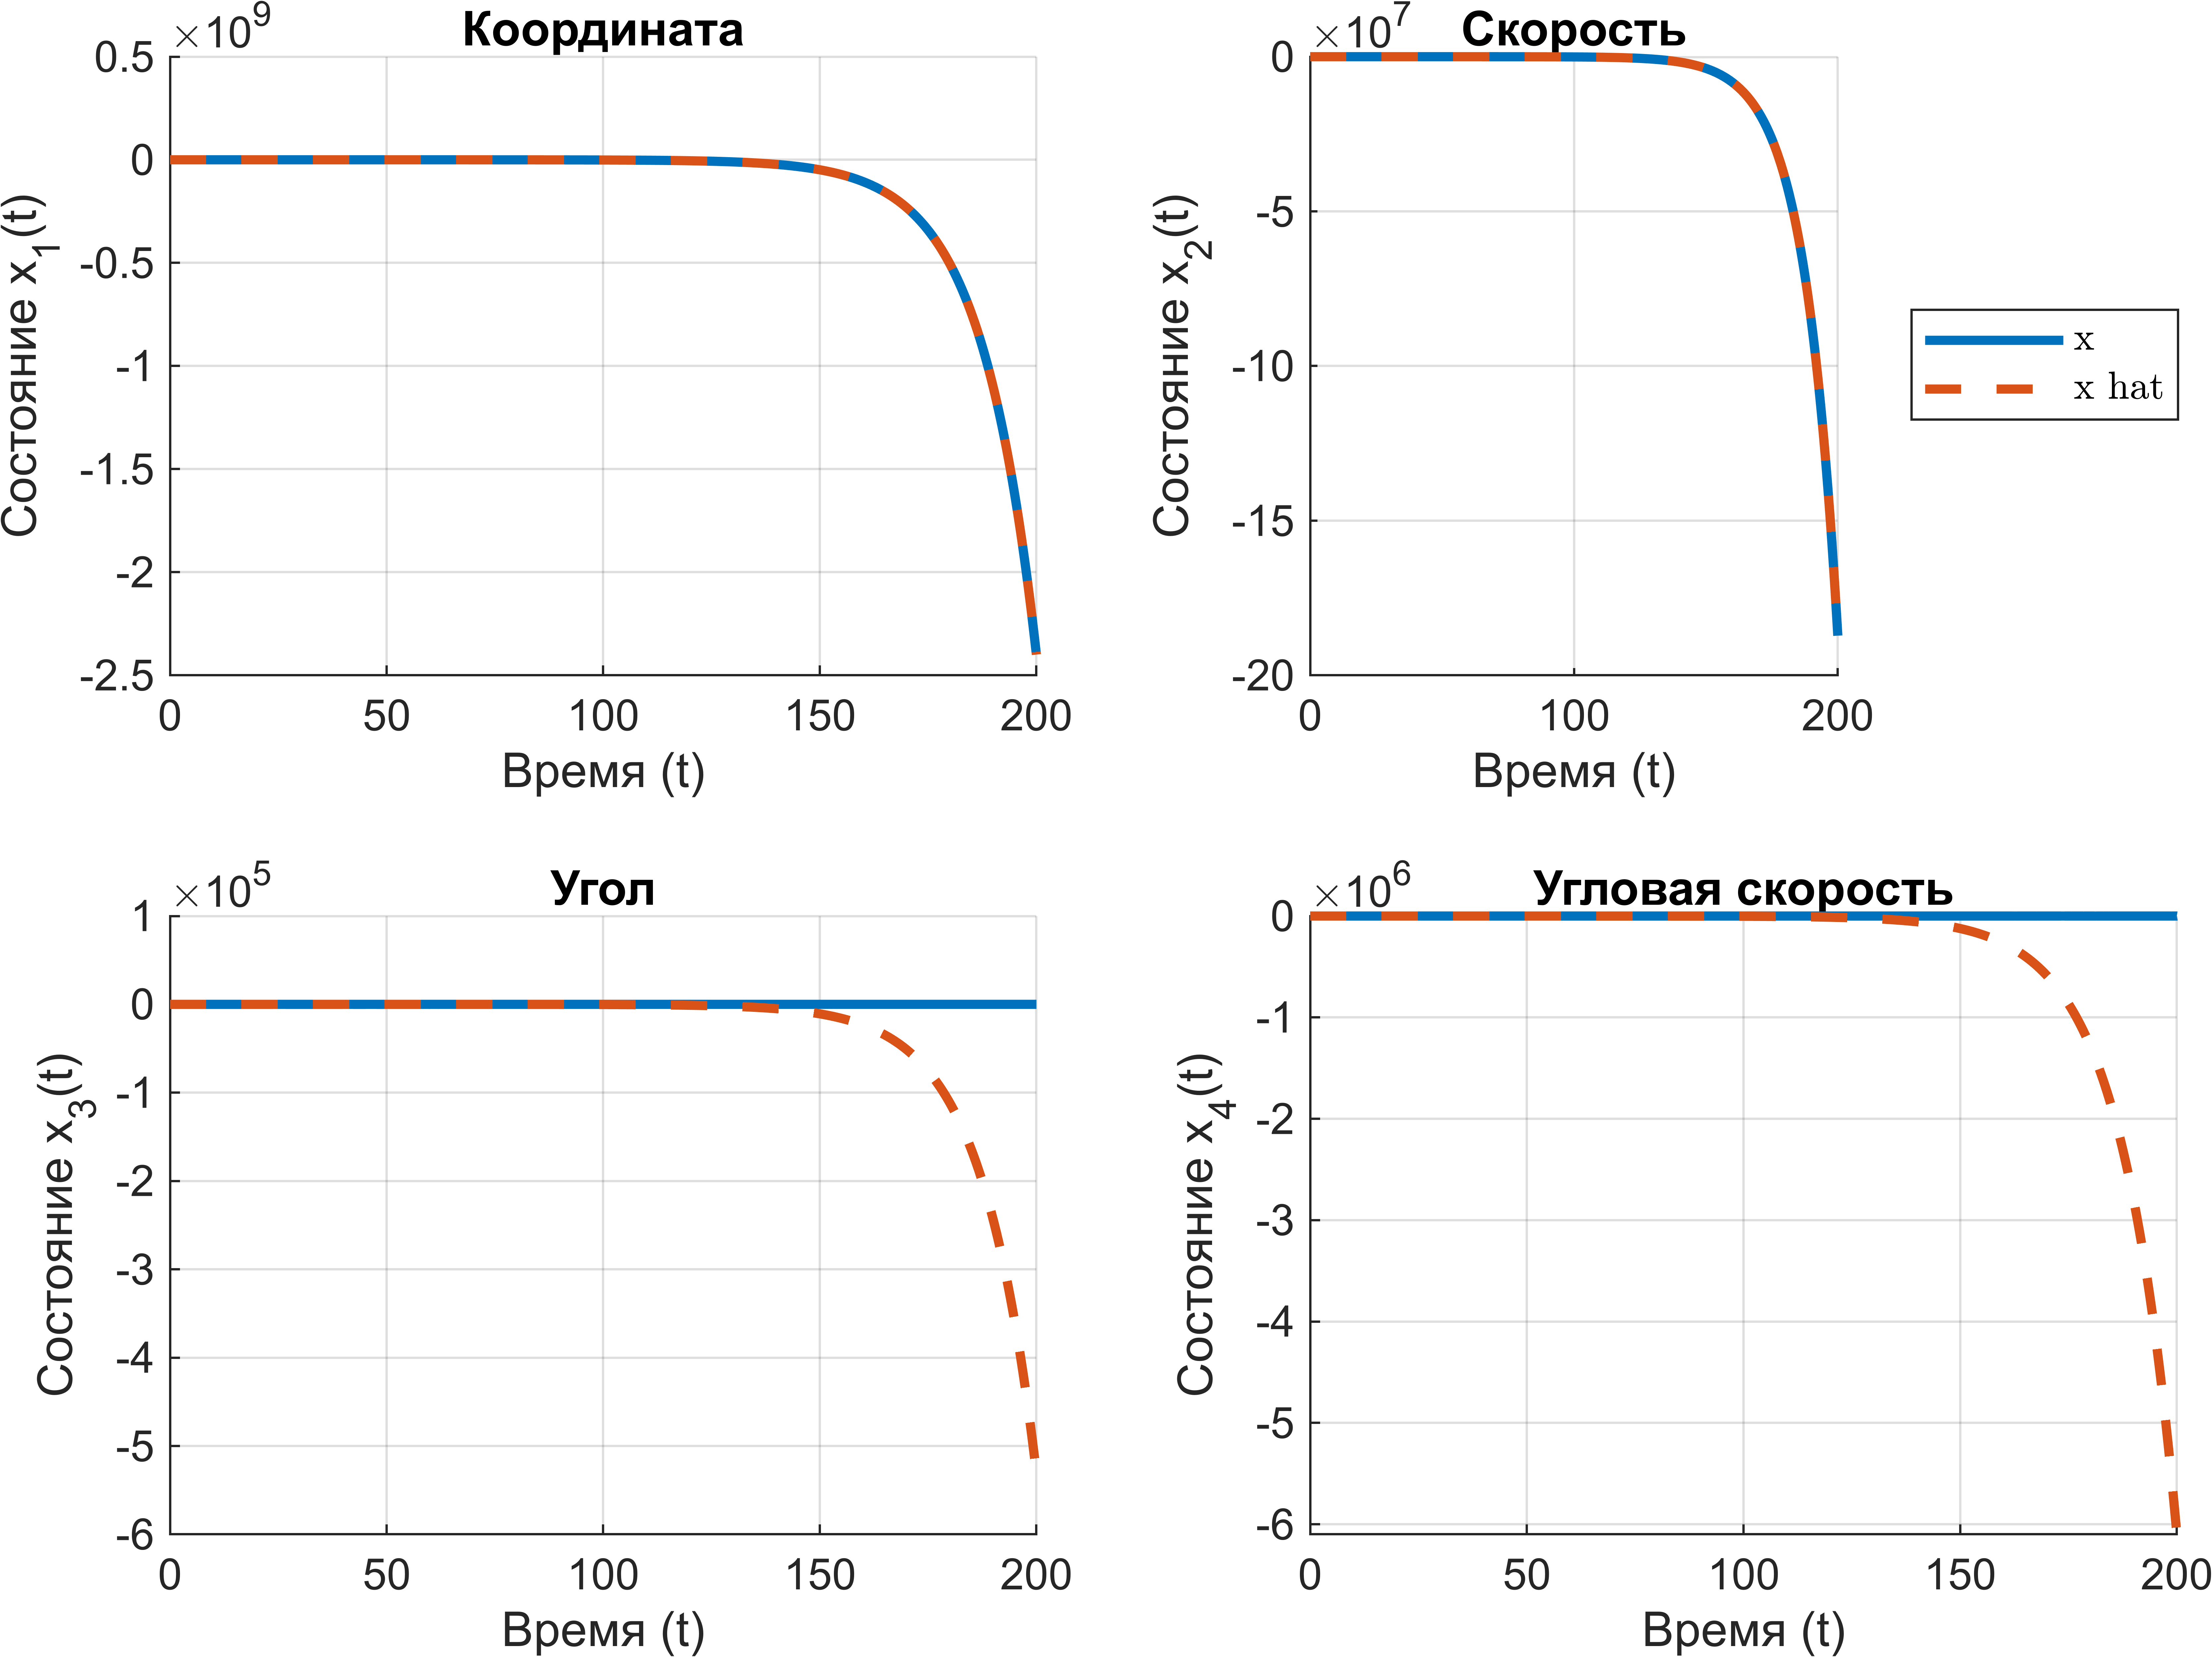
\includegraphics[width=0.7\linewidth]{figs/6.5.sim.1.png}
    \caption{Моделирование работы LQG при $L_1$}
    \label{fig:6.5.sim.1}
\end{figure}
\begin{figure}[H]
    \centering
    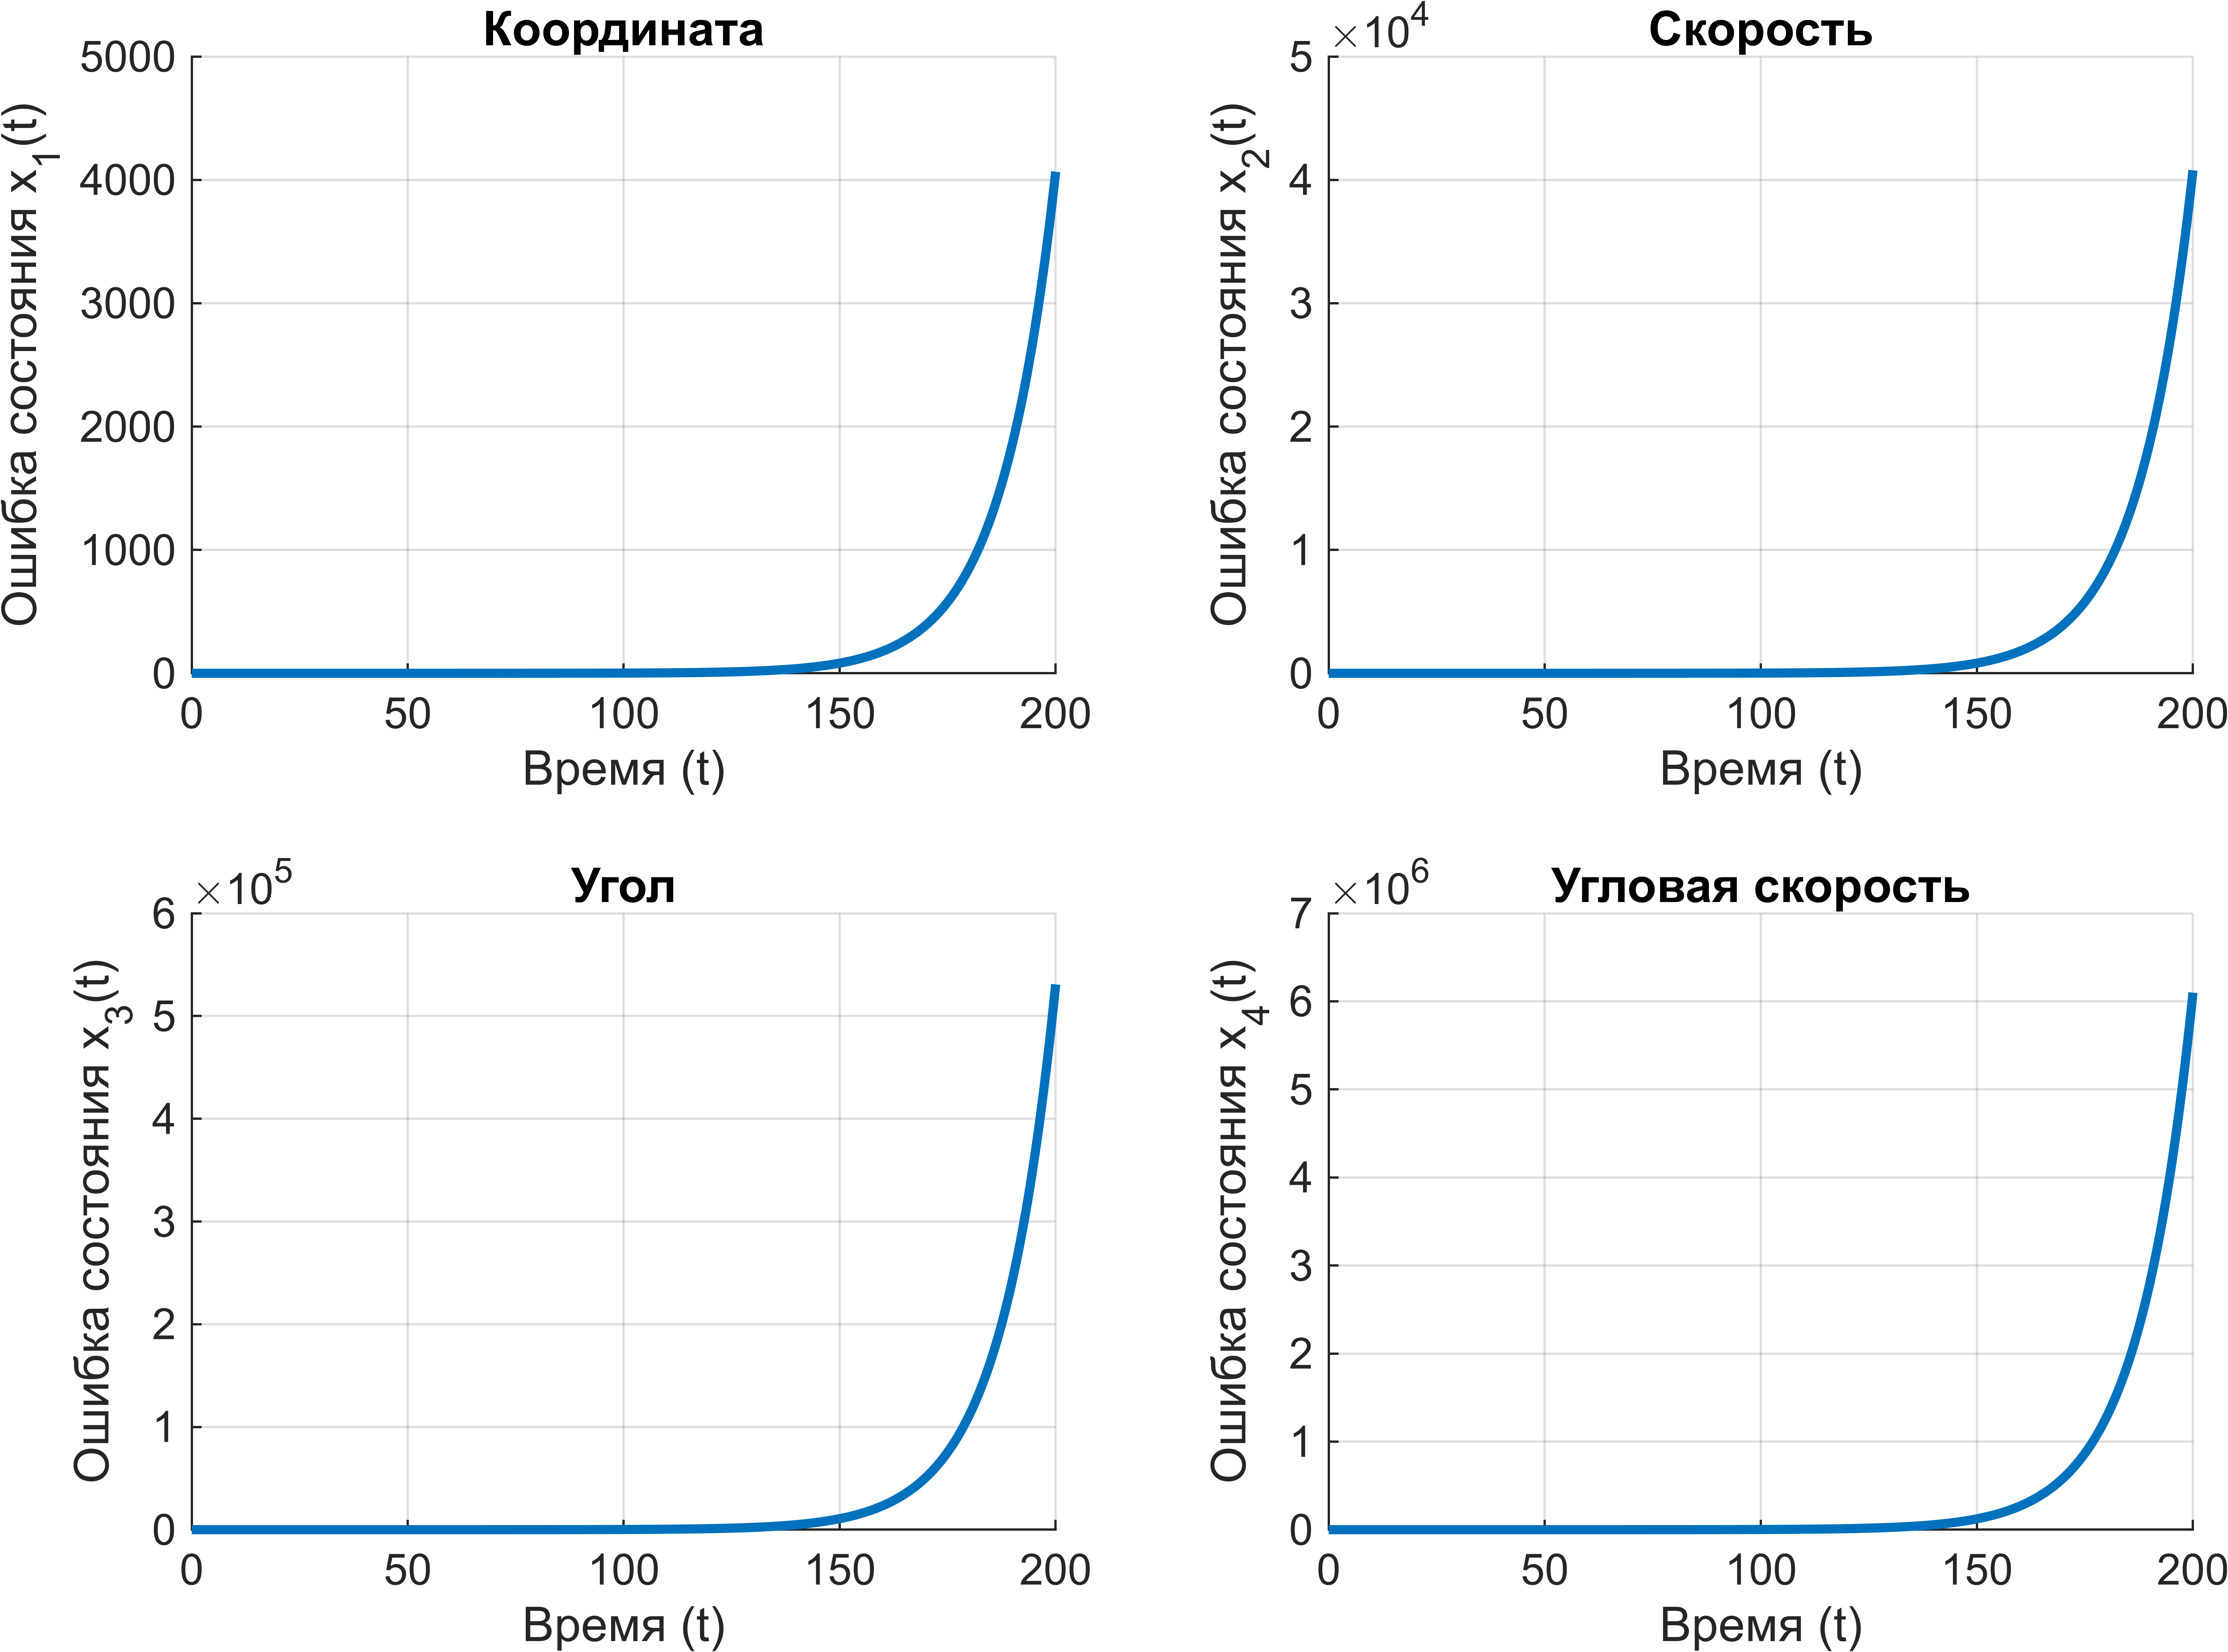
\includegraphics[width=0.7\linewidth]{figs/6.5.sim.1.err.png}
    \caption{Ошибка фильтра Калмана при $L_1$}
    \label{fig:6.5.sim.1.err}
\end{figure}
\begin{figure}[H]
    \centering
    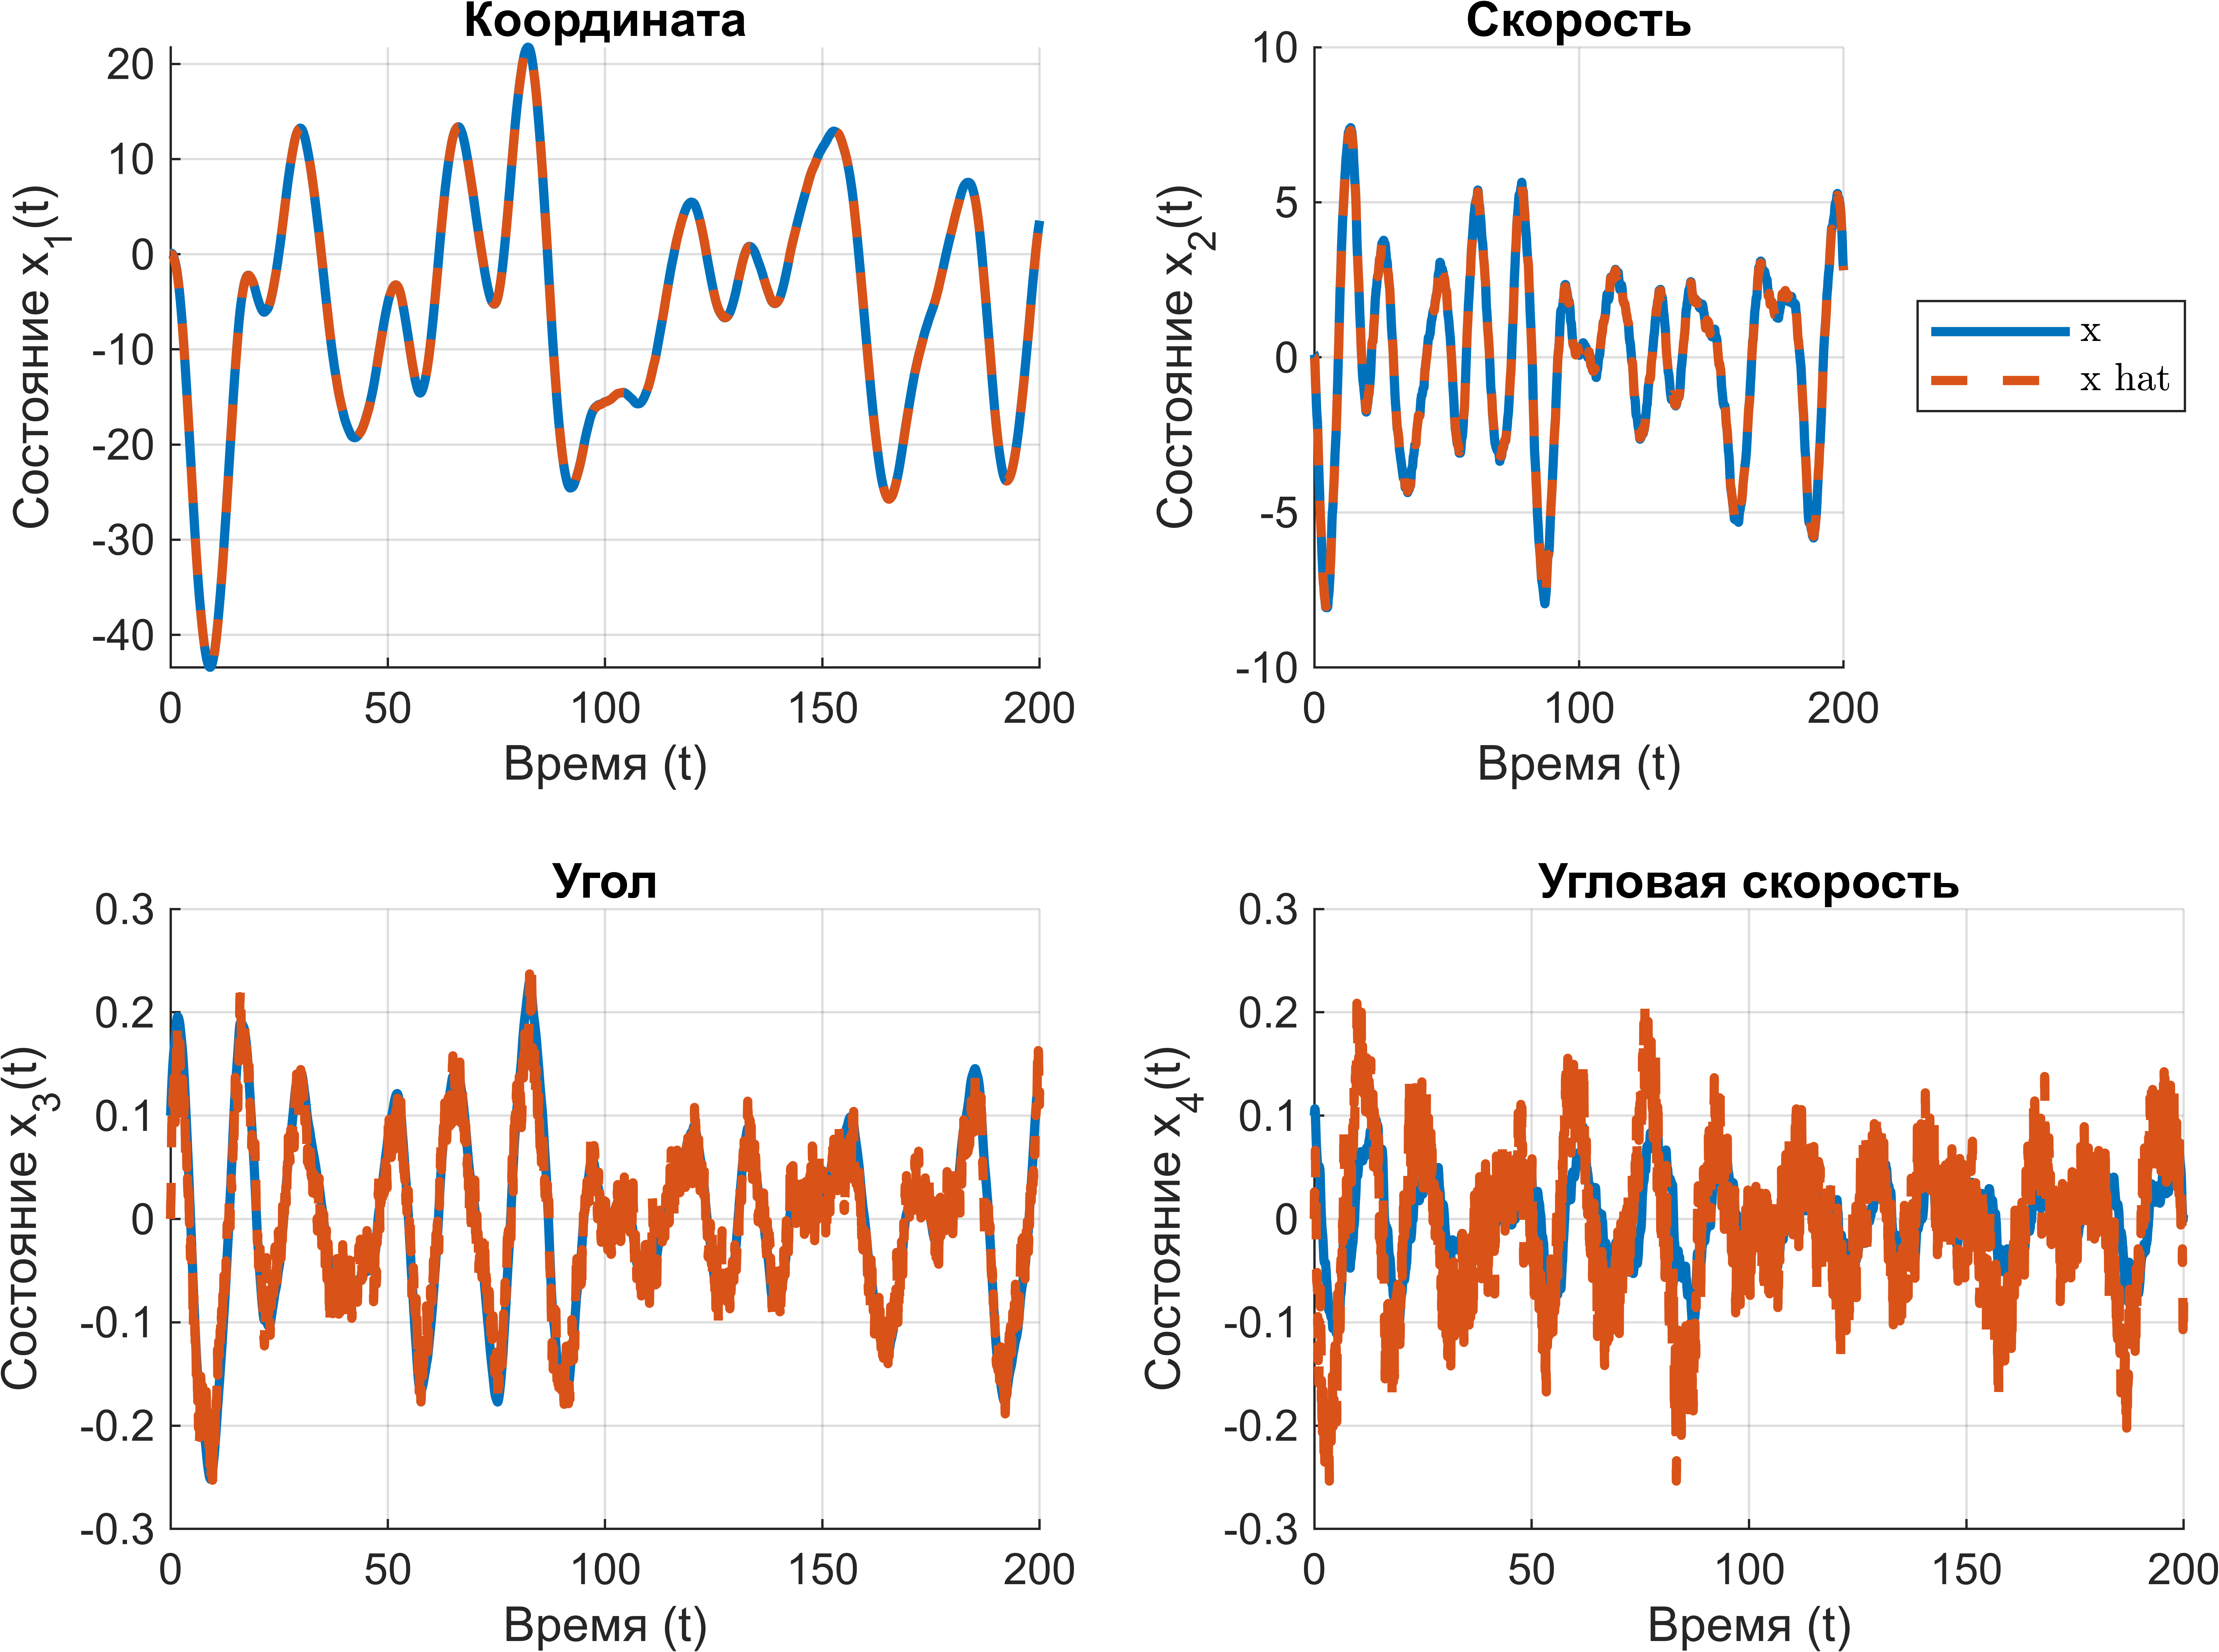
\includegraphics[width=0.9\linewidth]{figs/6.5.sim.2.png}
    \caption{Моделирование работы LQG при $L_2$}
    \label{fig:6.5.sim.2}
\end{figure}
\begin{figure}[H]
    \centering
    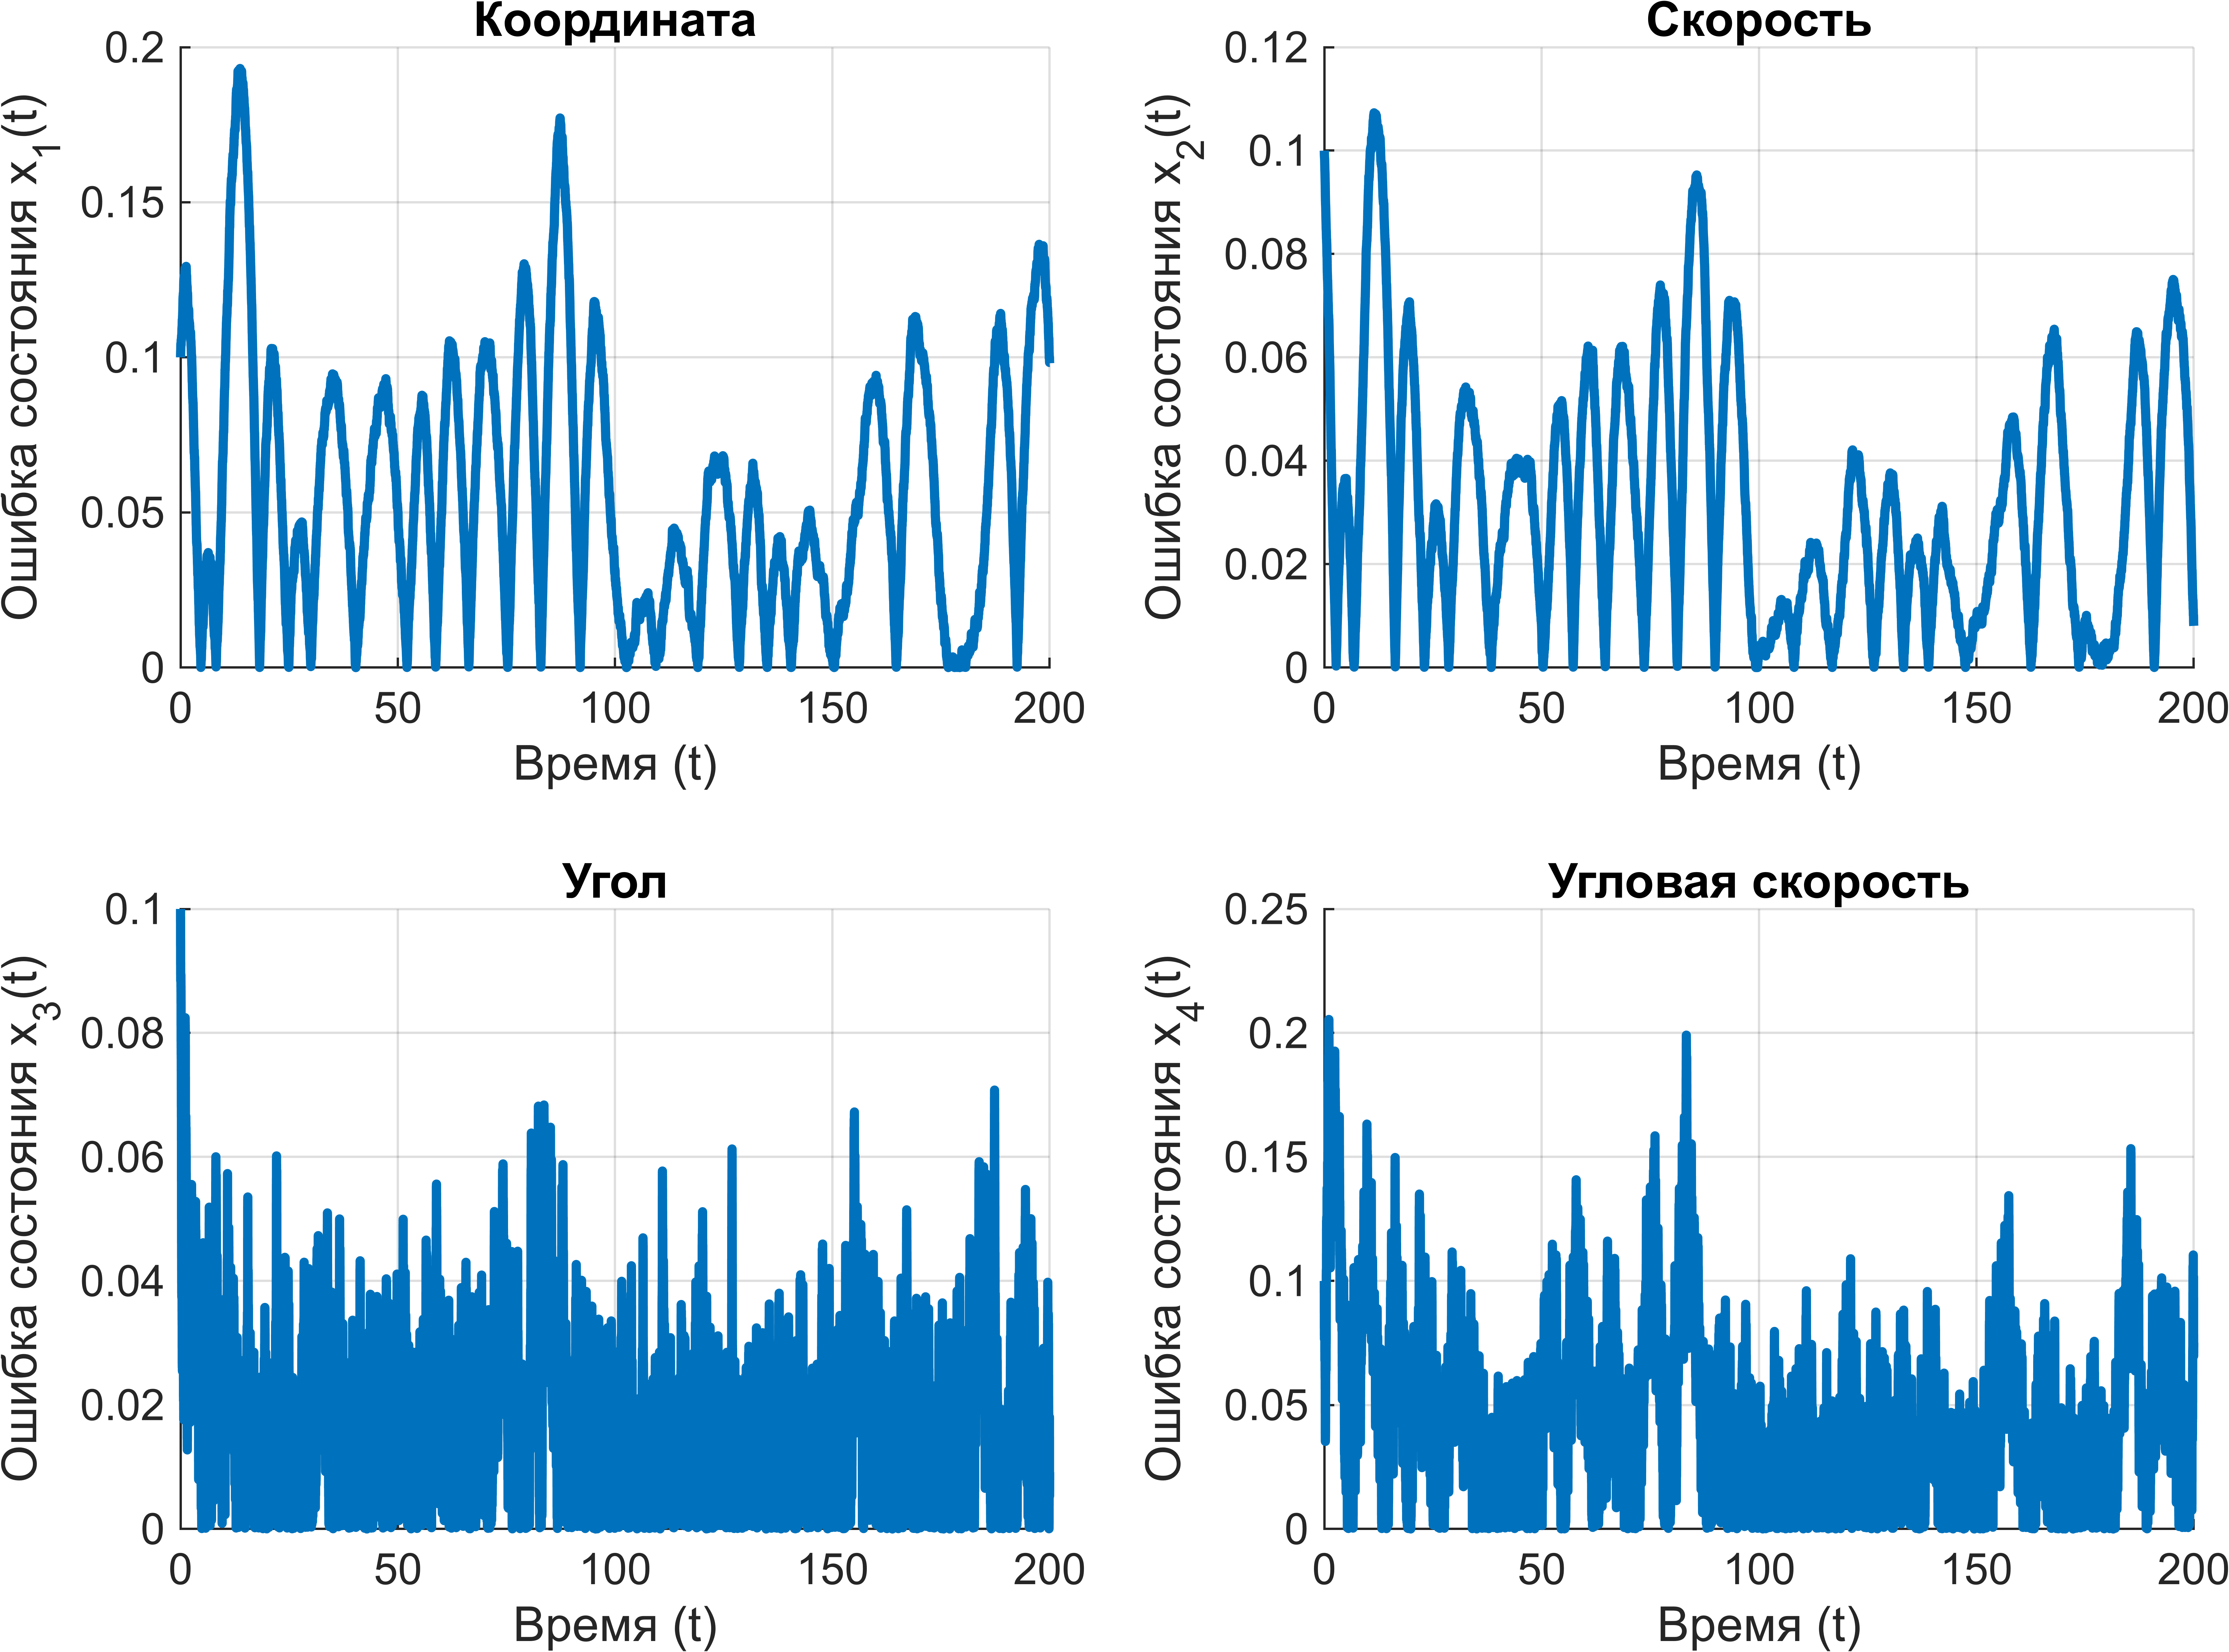
\includegraphics[width=0.9\linewidth]{figs/6.5.sim.2.err.png}
    \caption{Ошибка фильтра Калмана при LQG при $L_2$}
    \label{fig:6.5.sim.2.err}
\end{figure}

\chapter*{Заключение}

В ходе выполнения работы была построена и исследована математическая модель 
перевёрнутого маятника на тележке, а затем линеаризированна около верхнего неустойчивого 
положения равновесия, получены передаточные функции 
и исследованы их динамические свойства. Выполнено моделирование 
свободного движения как линеаризованной, так и нелинейной моделей.

Были синтезированы различные регуляторы: модальный, с заданной 
степенью устойчивости, с ограничением на управление, а также 
линейно-квадратичный (LQR). Для каждого из них проведён анализ 
влияния параметров на качество управления, исследованы области 
устойчивых начальных условий и затраты на управление. Показано, 
что увеличение быстродействия системы приводит к росту управляющего 
воздействия и колебательности, а введение ограничений на управление 
существенно сужает область допустимых начальных условий. Все эти регуляторы
успешно стаблизировали линейную и нелинейную системы при отсутствии 
внешних шумов.

Рассмотрены задачи компенсации и слежения, реализованы соответствующие 
регуляторы с генераторами гармонических сигналов. 
Проведено моделирование, подтверждающее работоспособность предложенных 
решений как для линейной, так и для нелинейной модели.

Синтезированы наблюдатели полного и пониженного порядка, а также 
фильтр Калмана, которые отлично работали как на нелинейной системе, так и на
линеаризированной. Реализована схема управления по 
выходу с использованием наблюдателей, а также LQG-регулятора для 
работы в условиях возмущений в состоянии и выходе представленных белым
гауссовским шумом. При LQG-регуляторе было показано, что
очень важно правильно выбирать матрицы $Q$ и $R$ для удержания объекта
в желаемом положении, было продемонстрированно различие между поведением 
нелинейной и линейной систем.

В результате работы показано, что задача стабилизации и управления 
перевёрнутым маятником может быть успешно решена используя методы
для линейных систем. Полученные результаты демонстрируют ограниченность
методов для линейных систем: при удалении объекта от точки равновесия, около
которой он был линеаризирован, ни один регулятор не смог вернуть маятник в 
верхнее положение.